\documentclass[UTF8,12pt,a4paper,oneside]{ctexbook}
\usepackage[margin=25mm]{geometry}
\usepackage{fontspec}
\setmainfont{Times New Roman}
\setsansfont{Times New Roman}
\setmonofont{DejaVu Sans Mono}
\setCJKmainfont[BoldFont=FandolSong-Bold.otf, ItalicFont=FandolKai-Regular.otf]{FandolSong-Regular.otf}
\setCJKsansfont[BoldFont=FandolHei-Bold.otf]{FandolHei-Regular.otf}
\setCJKmonofont[BoldFont=FandolHei-Bold.otf]{FandolHei-Regular.otf}
\usepackage{amsmath,amssymb,mathtools}
\usepackage{unicode-math}
\setmathfont{TeX Gyre Termes Math}
\usepackage{newunicodechar}
\newunicodechar{∅}{\ensuremath{\varnothing}}
\newunicodechar{ℰ}{\ensuremath{\mathcal{E}}}
\newunicodechar{ℒ}{\ensuremath{\mathscr{L}}}
\newunicodechar{ℜ}{\ensuremath{\mathfrak{R}}}
\newunicodechar{⋯}{\ensuremath{\cdots}}
\newunicodechar{∈}{\ensuremath{\in}}
\newunicodechar{⊗}{\ensuremath{\otimes}}
\newunicodechar{⊕}{\ensuremath{\oplus}}
\newunicodechar{∘}{\ensuremath{\circ}}
\newunicodechar{↦}{\ensuremath{\mapsto}}
\newunicodechar{∧}{\ensuremath{\wedge}}
\newunicodechar{∪}{\ensuremath{\cup}}
\newunicodechar{₁}{\textsubscript{1}}
\newunicodechar{₂}{\textsubscript{2}}
\newunicodechar{ₘ}{\textsubscript{m}}
\newunicodechar{ₚ}{\textsubscript{p}}
\newunicodechar{ₙ}{\textsubscript{n}}
\newunicodechar{ₖ}{\textsubscript{k}}
\usepackage{graphicx}
\usepackage{longtable,booktabs,array}
\usepackage{xcolor,framed,fancyvrb}
\usepackage{setspace}
\usepackage{enumitem}
\usepackage{microtype}
\usepackage[hidelinks,unicode,pdfusetitle,bookmarksnumbered]{hyperref}
\usepackage[open,openlevel=2]{bookmark}
\doublespacing
\setlength{\parindent}{1.5em}
\setlength{\parskip}{0pt}
\setcounter{tocdepth}{2}
\setcounter{secnumdepth}{2}
\setlist{itemsep=0.25\baselineskip,topsep=0.25\baselineskip}
\providecommand{\tightlist}{\setlength{\itemsep}{0pt}\setlength{\parskip}{0pt}}
\providecommand{\pandocbounded}[1]{#1}
\definecolor{shadecolor}{RGB}{248,248,248}
\newenvironment{Shaded}{\begin{snugshade}}{\end{snugshade}}
\newenvironment{Highlighting}[1][]{}{}
\newcommand{\NormalTok}[1]{#1\par}
\makeatletter
\def\maxwidth{\ifdim\Gin@nat@width>\linewidth\linewidth\else\Gin@nat@width\fi}
\def\maxheight{\ifdim\Gin@nat@height>0.8\textheight 0.8\textheight\else\Gin@nat@height\fi}
\makeatother
\setkeys{Gin}{width=\maxwidth,height=\maxheight,keepaspectratio}
\graphicspath{{images/}}
\emergencystretch=3em
\pagestyle{plain}
% Unnumbered front/back matter: starred heading, one TOC line, one bookmark
\newcommand{\specialchapter}[1]{\chapter*{#1}\phantomsection\addcontentsline{toc}{chapter}{#1}}
\newcommand{\specialsection}[1]{\section*{#1}\phantomsection\addcontentsline{toc}{section}{#1}}
% Sections are the §§ and number absolutely 1-15 across both parts;
% numbered items x.y are subsections. §8 follows the appendix chapter,
% so the section counter is restored by hand at the second part divider.
\renewcommand{\thesection}{\arabic{section}}
\title{微分流形与解析流形}
\author{尼古拉·布尔巴基}
\date{}
\begin{document}
\pagenumbering{gobble}
\maketitle
\clearpage
\frontmatter
\tableofcontents
\mainmatter
\specialchapter{警告}

这次重新印行的流形结果分册不加改动地重印了此前出版的著作（第 XXXIII 和 XXXXI 分册），并将它们汇编为一卷。

Nancago，1982 年秋

N. BOURBAKI

\part{第 1 至 7 段（97 页）}

\specialchapter{引言}

本分册汇集了可微流形（在实数域上）理论和解析流形（在完备非离散赋值域上）理论的基本概念与主要结果。不含证明。

假定已知前六卷的定义和结果。

\specialchapter{记号与约定（第 1 至 7 段）}

\specialsection{基域}

在本分册中，字母 K 表示以下三者之一：实数的赋值域 R、复数的赋值域 C，或带超度量绝对值的完备交换非离散赋值域（Top. Gen.，第 IX 章，第 3 版，第 3 节）。

\specialsection{拓扑向量空间}

当 K 不同于 R 或 C 时，我们把 K 上向量空间 F 的半范数（分别地，范数）称为 F 上的超半范数（分别地，作为范数的超半范数）（Esp. Vect. Top.，第 II 章，第 2 版，第 1 节）。若 γ 是 F 上的半范数且 x ∈ F，有时也写作 \textbar\textbar x\textbar\textbar γ 而不写 γ(x)。

我们把拓扑可由单个范数定义的 K 上拓扑向量空间称为可赋范空间，把完备的可赋范空间 \(^{1}\) 称为巴拿赫空间。我们把拓扑可由一族半范数定义的 K 上拓扑向量空间称为多范数空间；当 K = R 或 C 时，这一概念与局部凸空间的概念一致。

若 E 和 F 是多范数空间，我们用 \(\mathcal{L}_{m}(\mathrm{E};\mathrm{F})\) 表示从 \(m\) 到 F 的连续 \(\mathbf{E}^{m}\) 线性映射空间，并赋予其在 \(\mathbf{E}^{m}\) 的有界子集上一致收敛的拓扑；它是一个多范数空间。此外，若 E 可赋范，\(\gamma\) 是 F 上的连续半范数，且 \(u\in\mathcal{L}_{m}(\mathrm{E};\mathrm{F})\)，则以 \(\|u\|_{\gamma}\) 表示满足下列条件的实数 \(a\geqslant0\) 的下确界：

\[
\left\| u (x _ {1}, \dots , x _ {m}) \right\| _ {\gamma} \leqslant a \| x _ {1} \| \dots \| x _ {m} \|
\]

对 E 中所有的 \(x_{1}, \ldots, x_{m}\) 均成立。

\specialsection{多重指标}

设 I 为一集合。对于属于 \(\alpha = (\alpha_{i})\) 的 \(\beta = (\beta_{i})\) 和 \(\mathbf{N}^{(I)}\)，置（参见 Alg.，第 III 章，第 \(3^{\mathrm{e}}\) 版，章首）：

\[
| \alpha | = \sum_ {i \in I} \alpha_ {i}
\]

\[
\alpha ! = \prod_ {i \in I} \alpha_ {i}!
\]

\[
\alpha + \beta = (\alpha_ {i} + \beta_ {i}) _ {i \in I}
\]

\[
((\alpha , \beta)) = \prod_ {i \in I} \frac {(\alpha_ {i} + \beta_ {i}) !}{\alpha_ {i} ! \beta_ {i} !}.
\]

当对所有 \(\alpha \leqslant \beta\) 都有 \(\alpha_{i} \leqslant \beta_{i}\) 时，置 \(i \in I\)；这等价于存在 \(\gamma \in \mathbf{N}^{(I)}\) 使得 \(\beta = \alpha + \gamma\)；此时该元素 \(\gamma\) 唯一，记作 \(\beta - \alpha\)。

若 \(\mathbf{x} = (x_i)_{i \in I}\) 是环 A 中两两可交换的元素族，且 A 具有单位元 1，则置：

\[
\mathbf {x} ^ {\alpha} = \prod_ {i \in \mathbf {I}} x _ {i} ^ {\alpha_ {i}} \quad (\text { with   the   convention   that } x ^ {0} = 1).
\]

有 \(\mathbf{x}^{\alpha +\beta} = \mathbf{x}^{\alpha}\cdot \mathbf{x}^{\beta}\)。

对于 \(i\in I\)，用 \(\varepsilon_{i}\) 表示 \(\mathbf{N}^{(I)}\) 中除指标为 \(i\) 的坐标等于 1 外其余坐标全为零的元素。对于 \(\alpha=\sum_{i\in I}\alpha_{i}\varepsilon_{i}\) 中每个元素 \(\alpha=(\alpha_{i})\)，都有 \(\mathbf{N}^{(I)}\)。

\specialsection{映射的限制}

若 \(f\) 是从集合 \(A\) 到集合 \(B\) 的映射，且 \(C\) 是 \(A\) 的子集，则用 \(f|C\) 表示 \(f\) 对 \(C\) 的限制。

\specialsection{元素 ∞ 与 ω}

在整数集上添入两个记作 ∞ 和 ω 的元素。整数之间的序关系按如下约定扩充：

\[
n <   \infty <   \omega \quad \text { for   every   integer } n.
\]

置：

\[
\infty + n = n + \infty = \infty \quad \text { and } \quad \omega + n = n + \omega = \omega , \quad n \in \mathbf {Z}.
\]

字母 \(r\) 表示一个 \(\geqslant 1\) 的整数，或元素 \(\infty\)、\(\omega\) 之一。当 \(K \neq R\) 时，字母 \(r\) 总表示元素 \(\omega\)。当 \(r = \infty\)（分别地，当 \(r = \omega\)）时，对每个整数 \(r - k = r\) 置 \(k \geqslant 1\)。

\section{可微函数}

本节中，字母 E 表示 K 上的可赋范拓扑向量空间；字母 F 表示 K 上的分离多范数空间。

\subsection{点处两个函数的接触阶}

1.1.1. 设 X 为拓扑空间，\(\theta\) 为 X 中一点 \(x_0\) 的某邻域上定义的正数值函数。若函数 \(f\) 在 \(x_0\) 的某邻域上定义且取值于 F，并满足下列条件，则称 f 在 \(\theta\) 处相对于 \(x_0\) 可忽略：

对每个 \(\varepsilon > 0\) 以及 F 上每个连续半范数 \(\gamma\)，存在 \(F\) 的一个邻域 \(V\)\(x_0\)，使 \(f\) 和 \(\theta\) 在其上有定义，并且

\[
\| f (x) \| _ {\gamma} \leqslant \varepsilon \theta (x) \quad \text { for   every } x \in \mathbf {V}.
\]

要使 \(f\) 相对于 \(\theta\) 可忽略，只需对定义 F 的拓扑的一族半范数 \(\gamma\) 满足此条件即可。\(f\) 在 \(\theta\) 处相对于 \(x_{0}\) 是否可忽略，只取决于 \(f\) 和 \(\theta\) 在 \(x_{0}\) 处的芽。用 \(o_{x_{0}}(\theta)\)（当 \(o(\theta)\) 不会引起歧义时也写作 \(x_{0}\)）表示在 \(x_{0}\) 处相对于 \(\theta\) 可忽略的函数在 \(x_{0}\) 处的芽的集合：它是取值于 F 的映射在 \(x_{0}\) 处的芽空间的向量子空间。若 \(f\) 相对于 \(\theta\) 可忽略，按记号滥用，我们写 \(f \in o_{x_{0}}(\theta)\)，或者当 \(f(x) \in o(\theta(x))\) 趋于 \(x\) 时写 \(x_{0}\)。

若 \(f\) 和 \(g\) 是从 \(x_{0}\) 的某邻域到 \(F\) 的两个映射，且 \(f \equiv g \mod o(\theta)\) 相对于 \(f - g\) 可忽略，则也写作 f  g  o(\(\theta\))。

假设 K 等于 R 或 C，且 \(x_{0}\) 属于 X 中 \(\theta\) 有定义且非零的点集 Y 的闭包。此时关系 \(f \in o(\theta)\) 意味着：x 在 Y 中趋于 \(f(x)/\theta(x)\) 时，\(x_{0}\) 趋于 0，并且 \(\theta(x) = 0\) 蕴含 \(f(x) = 0\)。

1.1.2. 设 \(f\) 和 \(g\) 是在 \(F\) 中一点 \(x_0\) 的某邻域上定义且取值于 \(E\) 的两个函数。若 \(m\) 是正整数，且有下式，则称 \(f\) 和 \(g\) 在 \(\geqslant m\) 处的接触阶 \(x_0\)：

\[
f (x) - g (x) \in o (\| x - x _ {0} \| ^ {m}) \quad \text { for } x \text { tending   toward } x _ {0}
\]

无论选取何种范数来定义 E 的拓扑，均应如此。为此，只需对定义 E 的拓扑的某个范数验证上述关系即可。若如此，则有 \(f(x_0) = g(x_0)\)。

若 \(f\) 和 \(g\) 在 \(x_{0}\) 处取相同值，则称 \(f\) 和 \(g\) 在 \(x_{0}\) 处的接触阶为满足 \(+\infty\) 和 \(m\) 在 \(f\) 处接触阶 \(g\) 的整数 \(\geqslant m\) 的上确界（有限或等于 \(x_{0}\)）。

1.1.3. \(f\) 和 \(g\) 在 \(x_{0}\) 处的接触阶只取决于它们在点 \(x_{0}\) 处的芽。因此，可以谈论从 E 到 F 的两个映射芽 \(\varphi\) 和 \(\psi\) 在点 \(x_{0}\) 处的接触阶。关系 \(\langle\varphi\) 与 \(\psi\) 的接触阶 \(\geqslant m\rangle\) 是一个与向量结构相容的等价关系。

\subsection{点处的可微函数}

1.2.1. 设 \(f\) 在 E 中点 \(x_{0}\) 的某邻域上定义且取值于 F。若存在从 E 到 F 的连续仿射函数 \(f\)，使得 \(x_{0}\) 与 \(v\) 在 \(x_{0}\) 处的接触阶 \(\geqslant 1\)，则称 \(f\) 在 x＿0 处可微。此映射 \(v\) 唯一；存在唯一的从 E 到 F 的连续线性映射，记作 \(Df(x_{0})\)，使得：

\[
v (x) = v \left(x _ {0}\right) + D f \left(x _ {0}\right). \left(x - x _ {0}\right).
\]

若在 E 上选取一个范数，则这等价于：

\(f(x_0 + h) \equiv f(x_0) + Df(x_0).h \mod o(\|h\|)\)（其中 \(h\) 趋于 0），

这也可写成如下形式：

\[
\lim _ {h \rightarrow 0, h \neq 0} \frac {\| f (x _ {0} + h) - f (x _ {0}) - D f (x _ {0}) . h \| _ {\gamma}}{\| h \|} = 0
\]

对 F 上每个连续半范数 γ。

称 \(Df(x_{0})\) 中的元素 \(\mathcal{L}(\mathrm{E},\mathrm{F})\) 为 f 在 \(x_{0}\) 处的导数。有时用 \(D_{h}f(x_{0})\) 表示 \(Df(x_{0}).h\)。它是 F 中由下式定义的元素：

\[
\mathrm{D} _ {h} f (x _ {0}) = \lim _ {t \rightarrow 0, t \neq 0} \frac {f (x _ {0} + t h) - f (x _ {0})}{t}.
\]

1.2.2. 若函数 \(f\) 在 \(x_{0}\) 处可微，且对每个定义 E 的拓扑的范数都有下列关系，则称 f 在 \(x_{0}\) 处严格可微：

\[
f (y) - f (z) \equiv D f (x _ {0}). (y - z) \quad \text {   mod   } o (\| y - z \|)
\]

当 \((y, z)\) 在 \((x_0, x_0)\) 中趋于 \(E \times E\) 时成立。为此，只需对定义 \(E\) 的拓扑的某个范数满足此条件即可。此外，若 \(E\) 和 \(F\) 都是赋范空间，则对每个数 \(c > \|Df(x_0)\|\)，存在 \(x_{0}\) 的一个邻域 V，使得对 V 中的 y、z 有 \(\|f(y)-f(z)\|\leqslant c.\|y-z\|\)；这蕴含 f 在 V 中一致连续。

1.2.3. 函数 \(f\) 在 \(x_{0}\) 处可微或严格可微这一性质只取决于 \(f\) 在 \(x_{0}\) 处的芽。在 \(x_{0}\) 处可微的函数芽构成所有芽空间的向量子空间 \(\mathcal{V}\)，且从 \(f\mapsto\mathrm{D}f(x_{0})\) 到 \(\mathcal{V}\) 的映射 \(\mathcal{L}(\mathrm{E};\mathrm{F})\) 是线性的。在 \(x_{0}\) 处严格可微的函数芽构成 \(\mathcal{V}\) 的向量子空间。

1.2.4. 在 \(x_0\) 处可微的函数在 \(x_0\) 处连续。

1.2.5. 当 E = K 时，映射 \(u \mapsto u(1)\) 是从 \(\mathcal{L}(\mathbf{E}; \mathbf{F})\) 到 F 的同构；若函数 f 在 \(x_{0}\) 处可微，则元素

\[
f ^ {\prime} (x _ {0}) = \mathrm{D} f (x _ {0}). 1
\]

正是 Fonct. Var. Réelle，第 I 章，第 1 节，第 6 号注 2 中所给意义下的 \(f\) 在 \(x_0\) 处的导数。

\subsection{可微函数的复合}

1.3.1. 假设 F 可赋范。设 \(x_0 \in E\)、\(y_0 \in F\)，U 是 \(x_0\) 的一个邻域，V 是 \(y_0\) 的一个邻域；最后，设 \(f\) 是从 U 到 V 的映射，在 \(x_0\) 处可微，且 \(f(x_0) = y_0\)。若 \(g\) 是从 V 到分离多范数向量空间 G 的映射，在 \(y_0\) 处可微，则从 U 到 G 的映射 \(g \circ f\) 在 \(x_0\) 处可微，且有：

\[
\mathbf {D} (g \circ f) (x _ {0}) = \mathbf {D} g (y _ {0}) \circ \mathbf {D} f (x _ {0}).\tag{1}
\]

若 \(f\) 和 \(g\) 严格可微，则 \(g \circ f\) 也有同样结论。

1.3.2. 设 \(f\) 是在 E 中一点 \(x_0\)\(E\) 的某邻域上定义且取值于 \(F\) 的映射，并在 \(x_0\) 处可微；若 \(u\) 是从 \(F\) 到分离多范数空间 \(G\) 的连续线性映射，则函数 \(u \circ f\) 在 \(x_0\) 处可微，且有：

\[
\mathrm{D} (u \circ f) (x _ {0}) = u \circ \mathrm{D} f (x _ {0}).\tag{2}
\]

1.3.3. 假设 F 是分离多范数向量空间族 \((F_{i})_{i\in I}\) 的乘积；对 I 中每个 i，设 \(f_{i}\) 是在 E 中一点 \(x_{0}\) 的邻域 U 上定义且取值于 F 的映射，并令 \(f = (f_{i})_{i\in I}\)。f 在 \(x_{0}\) 处可微（分别地，严格可微）的充要条件是所有 \(f_{i}\) 都具有该性质；有：

\[
\mathrm{D} _ {h} f (x _ {0}) = (\mathrm{D} _ {h} f _ {i} (x _ {0})) _ {i \in \mathbf {I}} \quad \text { for   every } h \text { in } E.\tag{3}
\]

1.3.4. 若 E = K，则在公式 (1) 和 (3) 中可用 \(Df(x_{0})\) 替代 \(f'(x_{0})\)，用 \(D_{h}f_{i}(x_{0})\) 替代 \(f_{i}'(x_{0})\)。

\subsection{可微函数的乘积}

1.4.1. 设 \(F_{1}, \ldots, F_{m}\) 为分离多范数空间，u 为从 \(F_{1} \times \cdots \times F_{m}\) 到 F 的连续 m 线性映射。设 U 是 E 中一点 \(x_{0}\) 的邻域，\(f_{i}\) 是从 U 到 \(F_{i}\) 的映射（\(1 \leqslant i \leqslant m\)）。若 \(f_{i}\) 在 \(x_{0}\) 处可微（分别地，严格可微），则 \(u(f_{1}, \ldots, f_{m}) = g\) 也具有该性质，且有：

\[
\mathrm{D} _ {h} g (x _ {0}) = \sum_ {j = 1} ^ {m} u (f _ {1} (x _ {0}), \dots , \mathrm{D} _ {h} f _ {j} (x _ {0}), \dots , f _ {m} (x _ {0})) \quad \text { for } h \text { in } E, \tag {4}
\]

这可简写为：

\[
\mathrm{D} g = \sum_ {j = 1} ^ {m} u (f _ {1}, \dots , \mathrm{D} f _ {j}, \dots , f _ {m}).\tag{5}
\]

特别地，当 \(m = 2\) 时，有：

\[
\mathrm{D} u (f _ {1}, f _ {2}) = u (\mathrm{D} f _ {1}, f _ {2}) + u (f _ {1}, \mathrm{D} f _ {2}).\tag{6}
\]

当 \(m = 1\) 时，得到 1.3.2。

1.4.2. 当 E = K 时，在公式 (4) 至 (6) 中可用 \(g'\) 替代 Dg，用 \(Df_{j}\) 替代 \(f_{j}'\)。

\subsection{隐函数定理的第一类变体}

设 E 和 F 是巴拿赫空间，\(x_{0}\) 是 E 中一点，U 是 \(x_{0}\) 的一个邻域，f 是从 U 到 F 的映射。再设 f 在 \(x_{0}\) 处严格可微。

若 \(Df(x_0)\) 是从 E 到 F 的同构，则存在包含于 U 的 \(U_0\) 的开邻域 \(x_0\)，以及 \(V_0\) 的开邻域 \(f(x_0)\)，使得 \(f|U_0\) 是从 \(U_0\) 到 \(V_0\) 的同胚。逆于 \(g: V_0 \to U_0\) 的映射 \(f|U_0\) 在点 \(f(x_0)\) 处严格可微，且有：

\[
\mathrm{Dg} (f (x _ {0})) = \mathrm{Df} (x _ {0}) ^ {- 1}.
\]

1.5.2. 若 \(Df(x_{0})\) 是从 E 到 F 的满射，则存在包含于 U 的 \(U_{0}\) 的开邻域 \(x_{0}\)，使得 \(f|U_{0}\) 是开映射。

1.5.3. 若 \(Df(x_{0})\) 是单射且像为闭集，则存在包含于 U 的 \(U_{0}\) 的闭邻域 \(x_{0}\)，使得 \(f|U_{0}\) 是从 \(U_{0}\) 到 F 的闭子集的同胚。

\subsection{偏导数}

1.6.1. 设 \(f\) 在 \(U\) 中点 \(x_0\) 的邻域 \(E\) 上定义且取值于 \(F\)。设 \(X\) 是 \(E\) 的向量子空间，\(V\) 是 \(x\) 中满足 \(X\) 的点 \(x_0 + x \in U\) 的集合；对 \(g(x) = f(x_0 + x)\) 置 \(x \in V\)。若 \(f\) 在 0 处有导数，则称 \(X\) 在 \(x_0\) 处有关于 \(g\) 的偏导数；此导数记作 \(D_X f(x_0)\)；它是从 \(X\) 到 \(F\) 的连续线性映射。若 \(f\) 在 \(x_0\) 处可微，则 f 在 \(X\) 处有关于 \(x_0\) 的偏导数，且此偏导数是 \(Df(x_0)\) 对 \(X\) 的限制。

1.6.2. 假设 \(E\) 是有限个赋范向量空间 \(E_{i}\)（\(1 \leqslant i \leqslant n\)）的乘积，并将它们按规范方式识别为 \(E\) 的子空间；设 \(x_{0} = (x_{0}^{1}, \ldots, x_{0}^{n})\) 属于 \(E\)，\(U\) 是 \(x_{0}\) 中 \(E\) 的一个邻域；最后设 \(f\) 是从 \(U\) 到 \(F\) 的映射。若存在，则用 \(D_{i}f(x_{0})\) 表示在点 \(x_{0}^{i}\) 处的映射 \(z_{i} \mapsto f(x_{0}^{1}, \ldots, z_{i}, \ldots, x_{0}^{n})\) 的导数，该映射在 \(x_{0}^{i}\) 中 \(E_{i}\) 的某邻域上定义且取值于 \(F\)。这是 \(\mathcal{L}(E_{i}; F)\) 中的元素，称为 \(f\) 在 \(x_{0}\) 处的第 i 个偏导数。若 \(f\) 在 \(x_{0}\) 处可微，则 \(n\) 个偏导数均存在，并由下式确定 \(Df(x_{0})\)：

\[
\mathrm{D} f (x _ {0}). h = \sum_ {i = 1} ^ {n} \mathrm{D} _ {i} f (x _ {0}). h _ {i} \quad \text { for } h = (h _ {1}, \dots , h _ {n}) \text { in } E.
\]

1.6.3. 更具体地，令 \(E = K^{n}\)。若 f 在 \(x_{0}\) 处的偏导数存在，则用 \(\partial_{i}f(x_{0})\) 表示 F 中的元素 \(D_{i}f(x_{0}).1\)。常使用以下记号；假设已为 \(K^{n}\) 上的坐标函数选定记号，例如 \(u_{i}\) 表示从 \(K^{n}\) 到 K 的第 i 个投影。于是写作：

\[
\frac {\partial f}{\partial u _ {i}} \left(x _ {0}\right) \quad \text { or } \quad \left. \frac {\partial f}{\partial u _ {i}} \right| _ {x = x _ {0}}
\]

而不写 \(\partial_{i}f(x_{0})\)。

1.6.4. 令 \(E = K^{n}\)、\(F = K^{m}\)；设取值于 F 的函数 \(f = (f_{1}, \ldots, f_{m})\) 在 E 中点 \(x_{0}\) 处可微。偏导数 \(a_{ji} = \partial_{i} f_{j}(x_{0})\) 于是存在（它们是 K 中的元素）。由 \(a_{ji}\) 构成的 m 行 n 列矩阵（元素位于指标为 j 的行和指标为 i 的列）称为 f 在 \(x_{0}\) 处的雅可比矩阵；相对于这些空间的规范基，它是从 \(Df(x_{0})\) 到 \(K^{n}\) 的线性映射 \(K^{m}\) 的矩阵。

\subsection{迭代导数}

1.7.1. 设 \(f\) 在 E 中一点 \(x_{0}\) 的某邻域上定义且取值于 F。若 \(f\) 在 \(x_{0}\) 的某邻域上可微，则其导数 Df 是从 \(x_{0}\) 的某邻域到多范数空间 \(\mathcal{L}(\mathrm{E};\mathrm{F})\) 的映射，其中后者是从 E 到 F 的连续线性映射空间。设 \(p\) 是满足 \(\geqslant 2\) 的整数：

若 \(f\)\(p\) 在 \(x_0\) 的某邻域上可微，且其导数 \(f\) 在 \(x_0\) 处 \(Df\) 次可微，则称 \((p - 1)\) 在 \(x_0\) 处 \(p\) 次可微。于是定义 \(f\) 在 \(x_0\) 处的 \(p\) 阶导数；这是由下式定义的从 \(D^p f(x_0)\) 到 F 的连续 \(E^p\) 线性映射 \(F\)：

\[
\mathrm{D} ^ {p} f (x _ {0}). (h _ {1}, \dots , h _ {p}) = (\mathrm{D} (\mathrm{D} ^ {p - 1} f) (x _ {0}). h _ {1}). (h _ {2}, \dots , h _ {p}).
\]

此外置 \(D^{0}f = f\) 且 \(D^{1}f = Df\)。若 \(f\) 在 \(p\) 处 \(x_{0}\) 次可微，且 \(q\)、\(s\) 是满足 \(q + s = p\) 且 \(s > 0\) 的两个整数，则 \(f\) 在 \(q\) 的某邻域上 \(x_{0}\) 次可微，取值于 \(D^{q}f\) 的函数 \(\mathcal{L}_{q}(E; F)\) 在 \(s\) 处 \(x_{0}\) 次可微，并且有：

\[
\mathrm{D} ^ {q + s} f (x _ {0}). (h _ {1}, \dots , h _ {q + s}) = (\mathrm{D} ^ {s} (\mathrm{D} ^ {q} f) (x _ {0}). (h _ {1}, \dots , h _ {s})) \cdot (h _ {s + 1}, \dots , h _ {q + s})
\]

这一关系按记号滥用写成：

\[
\mathbf {D} ^ {q + s} f = \mathbf {D} ^ {s} \mathbf {D} ^ {q} f.
\]

1.7.2. 设 \((\mathbf{E}_{i})_{1\leqslant i\leqslant n}\) 是 E 的闭向量子空间，且 E 是各 \(E_{i}\) 的拓扑直和。于是，在存在时定义从 \(D_{i_{1}}\ldots D_{i_{m}}f\) 的某邻域到 F 的映射 f 的迭代偏导数 \(x_{0}\in E\)；它是从

\[
\mathbf {E} _ {i _ {1}} \times \dots \times \mathbf {E} _ {i _ {m}}
\]

到 F 的连续多线性映射，按整数 \(m \geqslant 1\) 归纳定义如下：若 \(D_{i_{2}} \ldots D_{i_{m}} f(x)\) 在 \(x_{0}\) 的某邻域上存在，且关于 \(E_{i_{1}}\) 有偏导数，则 \(D_{i_{1}} \ldots D_{i_{m}} f(x_{0})\) 由下式给出：

\[
\mathrm{D} _ {i _ {1}} \dots \mathrm{D} _ {i _ {m}} f (x _ {0}). (h _ {1}, \dots , h _ {m}) = (\mathrm{D} _ {i _ {1}} (\mathrm{D} _ {i _ {2}} \dots \mathrm{D} _ {i _ {m}} f) (x _ {0}). h _ {1}). (h _ {2}, \dots , h _ {m})
\]

其中 \(h_{k} \in E_{i_{k}}\)。

若 \(f\) 在 \(m\) 处 \(x_{0}\) 次可微，则偏导数 \(\mathbf{D}_{i_{1}}\ldots\mathbf{D}_{i_{m}}f(x_{0})\) 存在，并等于 \(\mathbf{D}^{m}f(x_{0})\) 对 \(\mathbf{E}_{i_{1}}\times\cdots\times\mathbf{E}_{i_{m}}\) 的子空间 \(\mathbf{E}^{m}\) 的限制。因此，\(\mathbf{D}^{m}f(x_{0})\) 完全由 \(m\) 处 \(x_{0}\) 阶迭代偏导数确定。

1.7.3. 假设 E 是有限维的，且 \((e_{1},\ldots,e_{n})\) 是 E 的一组基。置 \(E_{i}=Ke_{i}\)，并设 f 是从 \(x_{0}\) 的某邻域到 F 的映射。若偏导数 \(D_{i_{1}}\ldots D_{i_{m}}f(x_{0})\)（使用 1.7.2 的记号）存在，则置：

\[
\partial_ {i _ {1}} \dots \partial_ {i _ {m}} f (x _ {0}) = \mathbf {D} _ {i _ {1}} \dots \mathbf {D} _ {i _ {m}} f (x _ {0}). (e _ {i _ {1}}, \dots , e _ {i _ {m}}).
\]

\section{实可微函数}

本节假定 K = R。字母 E 表示 R 上的赋范向量空间；字母 F 表示 R 上的分离局部凸拓扑向量空间。

\subsection{点处的可微函数}

2.1.1. 设 \(f\) 在 E 中一点 \(x_{0}\) 的某邻域上定义且取值于 F。设 \(u\) 是从 E 到 F 的连续线性映射空间 \(\mathcal{L}(\mathrm{E};\mathrm{F})\) 中的元素。\(f\) 在 \(x_{0}\) 处可微且在那里以 \(u\) 为导数的充要条件是有

\[
\lim _ {h \rightarrow 0, h \neq 0} \frac {f (x _ {0} + h) - f (x _ {0}) - u (h)}{\| h \|} = 0.
\]

2.1.2. \(f\) 在 \(x_{0}\) 处严格可微的充要条件是有

\[
\lim_{\substack{(h,k)\to (0,0)\\ h\neq k}}\frac{f(x_{0} + h) - f(x_{0} + k) - \mathrm{D}f(x_{0})\cdot(h - k)}{\|h - k\|} = 0.
\]

2.1.3. 设 \(F_{1}\) 和 \(F_{2}\) 是两个分离局部凸空间，u 是从 \(F_{1} \times F_{2}\) 到 F 的双线性映射，并满足下列连续性条件：

(SC) 若 \(((a_{n}, b_{n}))\) 是 \(F_{1} \times F_{2}\) 中收敛于元素 \((a, b) \in \mathbf{F}_{1} \times \mathbf{F}_{2}\) 的元素序列，则序列 \((u(a_{n}, b_{n}))\) 在 F 中收敛于 \(u(a, b)\)。

设 \(f_{i}\)（\(i = 1, 2\)）是从 E 中一点 \(x_{0}\) 的某邻域到 \(F_{i}\) 的映射。若 \(f_{1}\) 和 \(f_{2}\) 在 \(x_{0}\) 处可微，则 \(u(f_{1}, f_{2})\) 在 \(x_{0}\) 处可微，且有：

\[
\mathbf {D} (u (f _ {1}, f _ {2})) (x _ {0}). h = u (\mathbf {D} f _ {1} (x _ {0}). h, f _ {2} (x _ {0})) + u (f _ {1} (x _ {0}), \mathbf {D} f _ {2} (x _ {0}). h)
\]

对所有 \(h \in E\) 均成立。

\subsection{中值定理}

2.2.1. 设 \(x,y\) 属于 \(E\)，\([x,y]\) 是连接这两点的闭线段。此外，设 \(f\) 是从 \([x,y]\) 的某邻域到空间 \(F\) 的映射，并在 \([x,y]\) 的每一点处可微。则 \(f(x)-f(y)\) 属于当 \(Df(z).(x-y)\) 遍历 \(z\) 时的点集 \([x,y]\) 的闭凸包。

2.2.2. 设 U 是 E 的连通开子集，f 是从 U 到
F 的映射，并在 U 的每一点处导数为零；则 f 在 U 上为常值。

2.2.3. 设 U 是 E 的凸开子集，f 是从 U 到 F 的映射，并在 U 的每一点处可微。给定 F 上的连续半范数 γ 和实数 M ≥ 0，下列条件等价：

\begin{enumerate}
\def\labelenumi{(\roman{enumi})}
\item
  对每个 \(x\)  \(\mathbf{U}\)，都有 \(\| Df(x)\|_{\gamma}\leqslant M\)。
\item
  对 U 中任意 \(x\) 和任意 \(y\)\(U\)，都有 \(\| f(x) - f(y)\|_{\gamma} \leqslant M . \| x - y\| \)。
\end{enumerate}

2.2.4. 设 U 是 E 中一点 \(x_0\) 的一个邻域，\(f\) 是在 U 去掉 \(x_0\) 的补集上定义且取值于 F 的函数。假设 \(f\) 在 U 中每个满足 \(Df(x)\) 的点 \(x\) 处都有导数 \(x \neq x_0\)，且函数 \(x \mapsto Df(x)\) 在 \(D_0\) 趋于 \(x\) 时有极限 \(x_0\)。那么，当  (E) \(\geqslant 2\) 时，\(f\) 在 \(x_0\) 处有极限，并且连续延拓到整个 U 的函数 \(f\) 在 x＿0 处可微、导数为 \(D_0\)；若 \(x_0\) 且假设 \(f\) 在 \(x_0\) 处有极限，同样结论也成立。

\subsection{\texorpdfstring{\(C^{r}\) 类函数 ( \(r \neq \omega\) )}{C\^{}\{r\} 类函数 (r ≠ ω)}}

2.3.1. 设 U 是 E 的开子集，f 是从 U 到 F 的映射。对 \(C^{r}\)，按 r 归纳如下定义关系“f 属于 \(r \in N\) 类”：

\begin{enumerate}
\def\labelenumi{\arabic{enumi})}
\item
  \(f\) 属于 \(\mathbf{C}^{0}\) 类，当且仅当 f 连续；
\item
  若 \(r\) 是整数且 r \(\geqslant 1\)，则函数 \(f\) 属于 \(\mathbf{C}^{r}\) 类，当且仅当它在 \(\mathbf{U}\)\(Df\) 的每一点处可微，且从 \(\mathbf{U}\) 到 \(\mathcal{L}(\mathbf{E};\mathbf{F})\) 的导数 Df 属于 \(\mathbf{C}^{r-1}\) 类。
\end{enumerate}

属于 C \(^{r}\) 类的函数也称为 r 次连续可微函数。

若 \(f\)\(\mathbf{C}^{\infty}\) 对每个整数 r 都属于 \(\mathbf{C}^{r}\) 类，则称 f 属于 \(r\) 类（或称无穷次可微）。

若 \(f\) 在 U 中属于 \(\mathbf{C}^{r}\) 类，则对每个整数 \(\mathbf{U}\)，\(f\) 都 \(p\)\(p \leqslant r\) 次可微，且函数 \(\mathbf{D}^{p}f\) 属于 \(\mathbf{C}^{r-p}\) 类。

2.3.2. 从 E 的开子集 U 到 F 的 \(C^{r}\) 类映射构成所有从 U 到 F 的映射空间的向量子空间 \(\mathcal{C}^{r}(U;F)\)。当 \(\mathcal{C}^{s}(U;F)\subset\mathcal{C}^{r}(U;F)\) 时，有 \(s\geqslant r\)。

2.3.3. 函数 \(f\) 在 E 的开子集 U 中属于 \(\mathbf{C}^{1}\) 类的充要条件是它在 U 的每一点处严格可微。

若 E 是赋范空间 \(E_{i}\) 的乘积，则从 E 的开集 V 到 F 的映射 \(f\) 属于 \(C^{r}\) 类，当且仅当对每个整数 m  r，\(f\) 的迭代偏导数 \(D_{i_{1}}\ldots D_{i_{m}}f\)\(m \leqslant r\) 都存在且连续。

2.3.4. 设 G 是赋范空间，U 是 E 的开子集。设 V 是 G 的开子集，\(g \in \mathcal{C}^{r}(U; G)\) 且 \(f \in \mathcal{C}^{r}(V; F)\)。若 \(g(U) \subset V\)，则从 U 到 F 的映射 \(f \circ g\) 属于 \(C^{r}\) 类。

设 \(\mathbf{F}_1\) 和 \(\mathbf{F}_2\) 是两个分离局部凸空间，\(u\) 是从 \(\mathbf{F}_1 \times \mathbf{F}_2\) 到 \(\mathbf{F}\) 的双线性映射，并且关于 \(\mathbf{F}_1\)（分别地，\(\mathbf{F}_2\)）的有界子集族是半连续的（Topological Vector Spaces，第 III 章，第 4 节，第 2 号）。设 \(\mathbf{U}\) 是 \(\mathbf{E}\) 的开子集，且 \(f_i \in \mathcal{C}^r(\mathbf{U};\mathbf{F}_i)\)（\(i = 1,2\)）。则函数 \(u(f_1,f_2)\) 属于 \(\mathcal{C}^r(\mathbf{U};\mathbf{F})\)。若 \(\mathbf{E}\) 有限维，只需假设 \(u\) 满足第 2.1.3 号的条件 (SC)。

2.3.5. 若 E 是赋范空间 \(E_{i}\)（\(1 \leqslant i \leqslant n\)）的乘积，且 f 是从 E 到 F 的连续 n 线性映射，则 f 属于 \(C^{\infty}\) 类，并且当 \(D^{p}f = 0\) 时有 \(p \geqslant n + 1\)。

2.3.6. 假设 E 和 F 是巴拿赫空间。设 f 是在 E 中一点 \(C^{r}\) 的某邻域上定义且取值于 F 的 \(r \geqslant 1\) 类函数（\(x_{0}\)）。设 \(y_{0} = f(x_{0})\)，并假设 \(Df(x_{0})\) 是从 E 到 F 的同构。则 f 诱导出一个从 \(x_{0}\) 的某邻域到 \(y_{0}\) 的某邻域的同胚 g（1.5），且 g 的逆映射在 \(C^{r}\) 的某邻域上属于 \(y_{0}\) 类。

\subsection{\texorpdfstring{\(C^{r}\) 类函数的导数}{C\^{}\{r\} 类函数的导数}}

2.4.1. 设 \(f\) 是从 E 的开集 U 到 F 的 \(\mathbf{C}^{r}\) 类映射。对每个 \(x \in \mathbf{U}\) 以及每个满足 \(s\)\(s \leqslant r\)  r 的整数 s，多线性映射 \(\mathbf{D}^{s}f(x)\) 都是对称的。

2.4.2. 再设 E 有限维，且 \((e_{1},\ldots,e_{n})\) 是 E 的一组基。偏导数 \(\partial_{i_{1}}\ldots\partial_{i_{s}}f\) 关于指标 \(i_{1},\ldots,i_{s}\) 对称地依赖。设指标 k 在序列 \(\alpha_{k}\) 中出现的次数为 \(i_{1},\ldots,i_{s}\)，并令 \(\alpha=(\alpha_{1},\ldots,\alpha_{n})\)。于是置：

\[
\partial^ {\alpha} f = \partial_ {1} ^ {\alpha_ {1}} \dots \partial_ {n} ^ {\alpha_ {n}} f = \partial_ {i _ {1}} \dots \partial_ {i _ {s}} f
\]

当相对于基 \((e_{1},\ldots,e_{n})\) 的坐标记为 \(x_{1},\ldots,x_{n}\) 时，也将 \(\partial^{\alpha}f\) 写成：

\[
\frac {\partial^ {| \alpha |} f}{\partial x _ {1} ^ {\alpha_ {1}} \dots \partial x _ {n} ^ {\alpha_ {n}}}
\]

\subsection{泰勒公式}

2.5.1. 设 \(r\) 是满足 r \(\geqslant 1\) 的整数，\(f\) 是从 E 的开集 U 到 F 的 \(C^r\) 类映射。对于 \(x \in U\)、\(h \in E\) 和 \(p \leqslant r\)，约定用 \(D^{p}f(x_0).h^p\) 代替 \(D^{p}f(x_0).(h,\ldots,h)\)。若线段 \([x,x + h]\) 包含于 U，则有公式（“泰勒公式”）：

\[
f (x + h) = \sum_ {p = 0} ^ {r - 1} \frac {1}{p !} \mathbf {D} ^ {p} f (x). h ^ {p} + v _ {r} (x; h)
\]

其中“余项” \(v_{r}(x; h)\) 由下式给出：

\[
v _ {r} (x; h) = \int_ {0} ^ {1} \frac {(1 - t) ^ {r - 1}}{(r - 1) !} \mathrm{D} ^ {r} f (x + t h). h ^ {r} d t
\]

有：

\[
v _ {r} (x; h) \equiv \frac {1}{r !} \mathrm{D} ^ {r} f (x). h ^ {r} \quad \text {   mod   } o (\| h \| ^ {r}) \quad \text {   when   } h \text {   tends   to   } 0
\]

以及

\[
f (x + h) \equiv \sum_ {p = 0} ^ {r} \frac {1}{p !} \mathrm{D} ^ {p} f (x). h ^ {p} \quad \mod o (\| h \| ^ {r})
\]

当 h 趋于零时。

2.5.2. 再设 \(\gamma\) 是 \(F\) 上的连续半范数；若对线段 \(\|D^{r}f(z)\|_{\gamma}\leqslant M\) 的每一点 \(z\) 都有 \([x,x + h]\)，则有：

\[
\| v _ {r} (x; h) \| _ {\gamma} \leqslant \frac {\mathbf {M}}{r !} \| h \| ^ {r}
\]

2.5.3. 再假设 \(\mathbf{E} = \mathbf{R}^n\)。于是有：

\[
f (x + h) \equiv \sum_ {| \alpha | \leqslant r} \Delta^ {\alpha} f (x) h ^ {\alpha} \quad \mod o (\| h \| ^ {r}) \text {   when   } h \text {   tends   to   } 0
\]

其中置：

\[
\Delta^ {\alpha} f (x) = \frac {1}{\alpha !} \partial^ {\alpha} f (x)
\]

2.5.4. 设 \(f\) 和 \(g\)\(C^r\) 是 E 的开集 \(U\)\(E\) 上取值于 \(F\) 的两个 C＾r 类函数。\(f\) 和 \(g\) 在 U 中一点 \(x\)\(U\) 处的接触阶 \(\geqslant r\) 的充要条件是，对每个满足 \(D^p f(x) = D^p g(x)\) 的整数 \(p\)，都有 \(0 \leqslant p \leqslant r\)。当 \(E\)\(\leqslant r\) 有限维时，这就是说 \(f\) 和 \(g\) 的  r 阶迭代偏导数（相对于 \(E\) 的一组基）在点 \(x\) 处相等。

2.5.5. 设 U 是 \(E \times R^{n}\) 的一个开子集，形如 \(V \times I_{1} \times \cdots \times I_{n}\)，其中 V 是 E 的开子集，\(I_{1}, \ldots, I_{n}\) 是包含 0 的 R 的开区间。置 \(U_{0} = V\)，并对 \(U_{j} = V \times I_{1} \times \cdots \times I_{j}\) 置 \(1 \leqslant j \leqslant n\)。给定函数 \(f \in \mathcal{C}^{r}(U; F)\)（\(1 \leqslant r \leqslant \infty\)），存在唯一的函数序列 \(f_{j}\in\mathcal{C}^{r-1}(\mathbf{U}_{j};\mathbf{F})\)（\(0\leqslant j\leqslant n\)），使得：

\[
f (x, t _ {1}, \dots , t _ {n}) = f _ {0} (x) + \sum_ {j = 1} ^ {n} t _ {j} f _ {j} (x, t _ {1}, \dots , t _ {j})
\]

对 \(x \in V\) 和 \(t_j \in I_j\) 成立。有：

\[
f _ {0} (x) = f (x, 0, \dots , 0)
\]

\[
f _ {j} (x, t _ {1}, \dots , t _ {j}) = \int_ {0} ^ {1} \partial_ {j} f (x, t _ {1}, \dots , t _ {j - 1}, t _ {j} u, 0, \dots , 0) d u
\]

对 \(1 \leqslant j \leqslant n\) 成立。在最后一个公式中，\(\partial_j f\) 表示函数 (t＿1, , t＿n)  f(x, t＿1, , t＿n) 的第 \(j\)\((t_1, \ldots, t_n) \mapsto f(x, t_1, \ldots, t_n)\) 个偏导数。

\subsection{可微性判据}

2.6.1. 假设 F 除了拓扑 T 外还赋有较粗拓扑 T'，且 T' 也使 F 成为分离局部凸空间。再假设 T 和 T' 满足下列条件：

\begin{enumerate}
\def\labelenumi{(\Alph{enumi})}
\setcounter{enumi}{18}
\tightlist
\item
  对 T 拓扑下 0 的每个邻域 V，都存在 T 拓扑下 0 的一个邻域 W，使得 W 的每个 T-紧子集的 T'-闭凸包都包含于 V。
\end{enumerate}

设 \(f\) 是从 E 的开子集 U 到 F 的映射。假设 F 赋予拓扑 T' 时 \(f\) 属于 \(\mathbf{C}^{r}\) 类（\(1 \leqslant r \leqslant \infty\)）；对 U 中所有 x 以及每个整数 \(\mathcal{T}'\)，\(\mathrm{D}^{m}f(x)\) 都是从 \(x\) 到赋予拓扑 \(m \leqslant r\) 的 F 的连续多线性映射；且映射 \(\mathrm{E}^{m}\) 从 U 到 \(\mathcal{T}\) 连续（F 赋予拓扑 \(x \mapsto \mathrm{D}^{m}f(x)\)\(\mathcal{L}_{m}(\mathrm{E};\mathrm{F})\)）。则 F 赋予拓扑 \(\mathcal{T}\) 时 \(f\) 属于 \(\mathbf{C}^{r}\)\(\mathcal{T}\) 类，并且其导数 \(\mathrm{D}^{m}f\) 对 \(\mathcal{T}\) 和 \(\mathcal{T}'\) 相同。

条件 (S) 特别地在如下情形成立：存在 T 拓扑下 0 的邻域基本系，其成员对拓扑 T' 都是闭的；当 F 赋予 T 时的对偶与 F 赋予 T' 时的对偶相同时，这一情形确实发生。若 F 赋予拓扑 T 时拟完备，条件 (S) 也成立（Topological Vector Spaces，第 III 章，第 2 节，第 5 号）。

2.6.2. 设 \(f\) 是从 E 的开集 \(U\)\(E\) 到 \(F\) 的映射。若 \(f\) 属于 \(C^r\) 类（\(0 \leqslant r \leqslant \infty\)），则对 F 上每个连续线性形式 u，标量函数 \(u \circ f\) 都属于 \(C^r\) 类。反之，若 F 拟完备，且对所有 \(u\)  \(F\)'，函数 \(u \circ f\) 都属于 \(C^{r+1}\)\(u \in F'\) 类，则 \(f\) 属于 \(C^r\) 类。

\section{实解析或复解析函数}

本段假定 K = R 或 C。用 \((\mathrm{E}_{i})\)（\(1 \leqslant i \leqslant n\)）表示 K 上赋范空间的一个有限族，用 E 表示各 \(E_{i}\) 的乘积空间，用 F 表示 K 上的分离局部凸拓扑向量空间。

\subsection{收敛级数}

3.1.1. 设 \(f = \sum f_{\alpha}\) 是属于 \(\hat{\mathbf{P}}(\mathbf{E}_1, \ldots, \mathbf{E}_n; \mathbf{F})\) 的形式级数（附录，第 A.5 号）。若 \(\gamma\) 是 \(\mathbf{F}\) 上的连续半范数，且 \(\mathbf{R} = (\mathbf{R}_1, \ldots, \mathbf{R}_n)\) 是 \(n\) 个严格正实数组成的序列，置：

\[
\| f \| _ {\gamma , \mathbf {R}} = \sum_ {\alpha} \mathbf {R} ^ {\alpha} \| f _ {\alpha} \| _ {\gamma}.
\]

若 \(F\) 是赋范空间且 \(\gamma\) 是 \(F\) 的范数，则用 \(\| f \|_{\mathbb{R}}\) 代替 \(\| f \|_{\gamma, \mathbb{R}}\)。

由满足对 \(\mathcal{H}_{\mathbb{R}}(\mathbf{E}_{1},\ldots,\mathbf{E}_{n};\mathbf{F})\) 上每个连续半范数 \(f\in\hat{\mathbf{P}}(\mathbf{E}_{1},\ldots,\mathbf{E}_{n};\mathbf{F})\)，\(\|f\|_{\gamma,\mathbb{R}}\) 都有限的 \(\gamma\) 构成的集合 \(\mathbf{F}\)，是 \(\hat{\mathbf{P}}(\mathbf{E}_{1},\ldots,\mathbf{E}_{n};\mathbf{F})\) 的向量子空间。有

\[
\mathcal {H} _ {\mathbb {R}} (\mathrm{E} _ {1}, \dots , \mathrm{E} _ {n}; \mathrm{F}) \subset \mathcal {H} _ {\mathbb {R} ^ {\prime}} (\mathrm{E} _ {1}, \dots , \mathrm{E} _ {n}; \mathrm{F})
\]

只要 \(R_{i} \geqslant R_{i}'\)（\(1 \leqslant i \leqslant n\)）即可。下列各空间的并

\[
\mathcal {H} _ {\mathbf {R}} (\mathrm{E} _ {1}, \dots , \mathrm{E} _ {n}; \mathrm{F})
\]

\(\mathcal{H}(E_{1},\ldots,E_{n};F)\)是 \(\hat{\mathrm{P}}(E_{1},\ldots,E_{n};F)\) 的向量子空间，记作 \(E_{i}\)，其中元素称为取值于 \(F\) 的各 \(E_{i}\) 的乘积上的收敛级数。它只取决于各 \(\mathcal{H}(E_{1},\ldots,E_{n};F)\) 的拓扑而不取决于它们的范数。因此，当各 \(E_{i}\) 是可赋范空间时，无须在每个 \(E_{i}\) 上选取范数，也可以谈论空间 H(E＿1,,E＿n;F)。

映射 \(f\mapsto\|f\|_{\gamma,\mathbb{R}}\) 是 \(\mathcal{H}_{\mathbb{R}}(\mathrm{E}_{1},\ldots,\mathrm{E}_{n};\mathrm{F})\) 上的半范数。当 \(\gamma\) 遍历 F 上的连续半范数（或仅遍历定义 F 的拓扑的一组半范数）时，由这些半范数定义的拓扑是豪斯多夫的。若 F 可赋范（分别地，完备），则 \(\mathcal{H}_{\mathbb{R}}(\mathrm{E}_{1},\ldots,\mathrm{E}_{n};\mathrm{F})\) 也可赋范（分别地，完备）。\(\mathcal{H}(\mathrm{E}_{1},\ldots,\mathrm{E}_{n};\mathrm{F})\) 上那些限制到每个 \(\mathcal{H}_{\mathbb{R}}\) 都连续的半范数，在 \(\mathcal{H}(\mathrm{E}_{1},\ldots,\mathrm{E}_{n};\mathrm{F})\) 上定义一个豪斯多夫拓扑，该拓扑只取决于各 \(\mathrm{E}_{i}\) 的拓扑。从 \(\mathcal{H}(\mathrm{E}_{1},\ldots,\mathrm{E}_{n};\mathrm{F})\) 到 \(\hat{\mathrm{P}}(\mathrm{E}_{1},\ldots,\mathrm{E}_{n};\mathrm{F})\) 的嵌入是连续的。

3.1.3. \(\hat{\mathbf{P}}(\mathbf{E};\mathbf{F})\) 到 \(\hat{\mathbf{P}}(\mathbf{E}_{1},\ldots,\mathbf{E}_{n};\mathbf{F})\) 的规范同构通过限制给出从 \(\mathcal{H}(\mathbf{E};\mathbf{F})\) 到 \(\mathcal{H}(\mathbf{E}_{1},\ldots,\mathbf{E}_{n};\mathbf{F})\) 的拓扑向量空间同构。

3.1.4. 设 \(f \in \mathcal{H}(\mathrm{E}_1, \ldots, \mathrm{E}_n; \mathrm{F})\)，并令 \(J(f)\)\(R \in (\mathbf{R}_+^*)^n\) 为满足 \(f \in \mathcal{H}_{\mathbb{R}}(\mathrm{E}_1, \ldots, \mathrm{E}_n; \mathrm{F})\) 的 \(I(f)\) 的集合。\(J(f)\) 的内部 I(\(f\)) 称为 f 的严格收敛指标。它由满足存在 \(R\)\(R' \in J(f)\)'  J(f) 且 \(0 < R_i < R'_i\)（\(1 \leqslant i \leqslant n\)）的 R 构成。用 \(\Omega(f)\)\((\log R_1, \ldots, \log R_n)\) 表示 R 属于 I(f) 时 \(R^n\) 中的点 \(R \in I(f)\) 的集合：它是 \(R^n\) 的凸子集。

当 \(n=1\) 时，集合 \(\mathbf{I}(f)\) 是 \([0,\rho(f)]\) 中的区间 \(\mathbf{R}\)，\(\rho(f)\) 称为 \(f\)\(+\infty\) 的严格收敛半径。它也是满足如下条件的实数 \(R>0\) 的集合的上确界（有限或 \(\gamma\)）：对 \(F\) 上每个连续半范数 ，存在常数 \(M\)，使得（其中 \(\|f_{m}\|_{\gamma}\leqslant MR^{-m}\)）对每个整数 \(f=\sum f_{m},f_{m}\in P_{m}(E;F)\) 都有 \(m\geqslant0\)。

满足存在 \(x = (x_i) \in \mathbf{E}_1 \times \cdots \times \mathbf{E}_n\) 且对所有 i 有 \(\mathbf{R} \in \mathbf{I}(f)\) 的点 \(\|x_i\| \leqslant R_i\) 的集合称为 f 的严格收敛域，记作 \(\mathbf{C}(f)\)。它也是满足存在 \(\mathbf{R} \in \mathbf{J}(f)\) 且对所有 i 有 \(\|x_i\| < R_i\) 的点 x 的集合的内部。

3.1.5. 对于 \(f_{\alpha} \in \mathbf{P}_{\alpha}(\mathbf{E}_1, \ldots, \mathbf{E}_n; \mathbf{F})\) 以及 \(\gamma\) 上每个连续半范数 \(\mathbf{F}\)，置：

\[
\| f _ {\alpha} \| _ {\gamma} = \sup _ {\| x _ {i} \| \leqslant 1} \| f _ {\alpha} (x _ {1}, \dots , x _ {n}) \| _ {\gamma}.
\]

于是有不等式：

\[
\left\| \left| f _ {\alpha} \right| \right\| _ {\gamma} \leqslant \left\| f _ {\alpha} \right\| _ {\gamma} \leqslant \frac {\alpha^ {\alpha}}{\alpha !} \left\| \left| f _ {\alpha} \right| \right\| _ {\gamma}.
\]

对于 \(f = \sum f_{\alpha} \in \hat{\mathbf{P}}(\mathrm{E}_1, \ldots, \mathrm{E}_n; \mathbf{F})\) 和 \(\mathbf{R} \in (\mathbf{R}_{+}^{*})^n\)，置：

\[
\| | f \| | _ {\gamma , \mathbf {R}} = \sum_ {\alpha} \mathbf {R} ^ {\alpha} \| | f _ {\alpha} \| | _ {\gamma}
\]

并用 \(\tilde{\mathcal{H}}_{\mathbb{R}}(\mathrm{E}_{1},\ldots ,\mathrm{E}_{n};\mathrm{F})\) 表示下列空间的向量子空间

\[
\hat {\mathbf {P}} (\mathbf {E} _ {1}, \dots , \mathbf {E} _ {n}; \mathbf {F})
\]

由满足对每个  都有  | \(f\)\(\| | f \| | _ {\gamma,\mathbb{R}}\)  | ＿ \(\gamma\),R 有限的 f 构成，并赋予由半范数 \(f\mapsto\| | f \| | _ {\gamma,\mathbb{R}}\) 定义的拓扑。有 \(\mathcal{H}_{\mathbb{R}}\subset\tilde{\mathcal{H}}_{\mathbb{R}}\)，且从 \(\mathcal{H}_{\mathbb{R}}\) 到 \(\tilde{\mathcal{H}}_{\mathbb{R}}\) 的嵌入是连续的。空间 \(\mathcal{H}(\mathrm{E}_{1},\ldots,\mathrm{E}_{n};\mathrm{F})\) 是各 \(\tilde{\mathcal{H}}_{\mathbb{R}}(\mathrm{E}_{1},\ldots,\mathrm{E}_{n};\mathrm{F})\) 的并，其拓扑是使 \(\mathcal{H}_{\mathbb{R}}\) 到 \(\mathcal{H}\) 的嵌入连续的最细局部凸拓扑。

若 \(f \in \mathcal{H}(E_1, \ldots, E_n; F)\)，则称满足 \(\tilde{I}(f)\) 的 \(\tilde{J}(f)\) 的集合 \(R \in (\mathbf{R}_+^*)\) 的内部 \(f \in \mathcal{H}_{\mathbb{R}}\) 为收敛指标。有：

\[
e ^ {- 1} \mathbf {I} (f) \subset \tilde{\mathbf {I}} (f) \subset \mathbf {I} (f)
\]

（其中 e 是自然对数的底）。从 \(\tilde{I}(f)\) 出发，按 3.1.4 定义收敛域 \(\tilde{C}(f)\)，并在 \(n = 1\) 时定义收敛半径 \(\tilde{\rho}(f)\)。特别地，有：

\[
e ^ {- 1} \tilde {\rho} (f) \leqslant \rho (f) \leqslant \tilde {\rho} (f).
\]

3.1.6. 对于 \(\mathbf{R} \in (\mathbf{R}_{+}^{*})^{n}\)，将 E 中以 0 为中心、半径为 \(\mathbf{R}\) 的（闭）多球称为由满足对所有 i 都有 \(\mathbf{B}(\mathbf{R})\) 的 \(x \in \mathbf{E}\) 构成的集合 \(\|x_{i}\| \leqslant \mathbf{R}_{i}\)。若  E＿\(i\)\(\dim \mathbf{E}_{i} = 1\) = 1，也称为多圆盘。若 \(f \in \mathcal{H}(\mathbf{E}_{1}, \ldots, \mathbf{E}_{n}; \mathbf{F})\)，则 \(f\) 的收敛域（分别地，严格收敛域）是 \(\mathbf{B}(\mathbf{R})\)（分别地，\(\mathbf{R} \in \tilde{\mathbf{I}}(f)\)）时多球 \(\mathbf{R} \in \mathbf{I}(f)\) 的并。

3.1.7. 设 \(f \in \mathcal{H}(E_1, \ldots, E_n; F)\)。假设 F 拟完备。对每个 \(x \in \tilde{\mathbf{C}}(f)\)，族 \(f_{\alpha}(x)\) 在 F 中可求和。其和记作 \(\hat{f}(x)\)，或简写为 \(f(x)\)，是 \(\tilde{\mathbf{C}}(f)\) 上的连续函数。更确切地说，对每个满足 \(f \in \tilde{\mathcal{H}}_{\mathbb{R}}\) 的 R，族 \(f_{\alpha}(x)\) 当 \(x \in B(R)\) 时一致可求和。映射 \(f \mapsto \hat{f}\) 是从 \(\tilde{\mathcal{H}}_{\mathbb{R}}\) 到 \(B(R)\) 上有界连续函数空间的连续线性单射，后者赋予一致收敛拓扑。

3.1.8. 设 \(F_1, \ldots, F_m\) 是分离多范数空间，\(u\)\(m\) 是从 \(F_1 \times \cdots \times F_m\) 到 \(F\) 的连续 m 线性映射。设 \(f_i \in \mathcal{H}(E_1, \ldots, E_n; F_i)\)（\(1 \leqslant i \leqslant m\)）。形式级数 \(u(f_1, \ldots, f_m)\) 属于 \(\mathcal{H}(E_1, \ldots, E_n; F)\)。有：

\[
\mathrm{C} (u (f _ {1}, \dots , f _ {m})) \supset \bigcap_ {i} \mathrm{C} (f _ {i})
\]

\[
\tilde {C} (u (f _ {1}, \dots , f _ {m})) \supset \bigcap_ {i} \tilde {C} (f _ {i})
\]

并且，若 \(x \in \bigcap_{i} \tilde{C}(f_i)\)，且 F 和各 \(F_i\) 拟完备，则有：

\[
u (f _ {1}, \dots , f _ {m}) (x) = u (f _ {1} (x), \dots , f _ {m} (x)).
\]

3.1.9. 设 \(\mathbf{F}_1, \ldots, \mathbf{F}_m\) 是完备赋范空间，且 \(\mathbf{F}\) 拟完备。令 \(\mathbf{f} = (f_i)_{1 \leqslant i \leqslant m}\)，其中 \(f_i \in \mathcal{H}(\mathbf{E}_1, \ldots, \mathbf{E}_n; \mathbf{F}_i)\)，\(g \in \mathcal{H}(\mathbf{F}_1, \ldots, \mathbf{F}_m; \mathbf{F})\)，并假设 \((f_i(0))_{1 \leqslant i \leqslant m}\) 属于 \(g\) 的严格收敛域。于是，对每个 \(\alpha \in \mathbb{N}^m\)，形式级数 \(g_\alpha \circ \mathbf{f}\) 属于 \(\mathcal{H}(\mathbf{E}_1, \ldots, \mathbf{E}_n; \mathbf{F})\)，且族 \(g_\alpha \circ \mathbf{f}\) 在 \(\mathcal{H}(\mathbf{E}_1, \ldots, \mathbf{E}_n; \mathbf{F})\) 中可求和，从而当然也在 \(\hat{\mathbf{P}}(\mathbf{E}_1, \ldots, \mathbf{E}_n; \mathbf{F})\) 中可求和。其和记作 \(g \circ \mathbf{f}\)。

更确切地说，存在 \(\mathbb{R}\in\bigcap_{i}\mathrm{I}(f_{i})\) 和 \(\mathbb{R}^{\prime}\in\mathrm{I}(g)\)，使得当 \(\|f_{i}\|_{\mathbb{R}}<R_{i}^{\prime}\) 时 \(1\leqslant i\leqslant m\)。在这些条件下，形式级数 \(g_{\alpha}\circ f\) 属于 \(\mathcal{H}_{\mathbb{R}}(\mathrm{E}_{1},\ldots,\mathrm{E}_{n};\mathrm{F})\)，且族 \(g_{\alpha}\circ f\) 在 \(\mathcal{H}_{\mathbb{R}}(\mathrm{E}_{1},\ldots,\mathrm{E}_{n};\mathrm{F})\) 中可求和。最后，若 \(x\in\mathrm{B}(\mathbb{R})\)，则 \(\mathbf{f}(x)=(f_{i}(x))\) 属于 \(\mathrm{B}(\mathrm{R}^{\prime})\subset\mathrm{F}_{1}\times\cdots\times\mathrm{F}_{m}\)，且有：

\[
g (\mathbf {f} (x)) = (g \circ \mathbf {f}) (x).
\]

3.1.10. 假设 \(E_{i} = K\)（\(1 \leqslant i \leqslant n\)）。于是将空间 \(\hat{\mathbf{P}}(\mathbf{K}^{n}; \mathbf{F})\) 识别为具有 F 中系数的 n 个不定元 \(X_{1}, \ldots, X_{n}\) 的形式幂级数空间，且 \(\hat{\mathbf{P}}(\mathbf{K}^{n};\mathbf{F})\) 中的元素写作：

\[
f = \sum_ {\alpha} X ^ {\alpha} c _ {\alpha} \quad \text {   with   } c _ {\alpha} \in F.
\]

若 \(\mathbf{R} \in (\mathbf{R}_{+}^{*})^{n}\)，且 \(\gamma\) 是 \(\mathbf{F}\) 上的连续半范数，则有：

\[
\| | f \| | _ {\gamma , \mathbf {R}} = \| f \| _ {\gamma , \mathbf {R}} = \sum_ {\alpha} \mathbf {R} ^ {\alpha} \| c _ {\alpha} \| _ {\gamma}
\]

有 \(\mathbf{I}(f) = \tilde{\mathbf{I}}(f)\)、\(\mathbf{C}(f) = \tilde{\mathbf{C}}(f)\)，并且当 \(n = 1\) 时 \(\rho(f) = \tilde{\rho}(f)\)。

系数在 \(\mathcal{H}(\mathbf{K}^{n};\mathbf{K})\) 中的收敛级数空间 \(\mathbf{K}\) 也记作 \(\mathbf{K}\{\{\mathbf{X}_{1},\ldots ,\mathbf{X}_{n}\}\}\)；它是 \(\mathbf{K}[[\mathbf{X}_1,\dots ,\mathbf{X}_n]]\) 的子代数。空间 \(\mathcal{H}(\mathbf{K}^n;\mathbf{F})\) 是 \(\mathbf{K}\{\{\mathbf{X}_1,\ldots ,\mathbf{X}_n\}\}\) 上的模；若 \(\mathbf{F}\) 有限维，则将此模识别为 \(\mathbf{K}\{\{\mathbf{X}_1,\ldots ,\mathbf{X}_n\}\} \otimes_{\mathbf{K}}\mathbf{F}\)。

3.1.11. 设 \(\mathbf{f} \in \mathcal{H}(\mathbf{K}^n; \mathbf{K}^m)\)，它由系数在 K 中的 \(m\) 个收敛级数 \(f_j(X_1, \ldots, X_n)\) 组成的系统表示。同样，设 \(\mathbf{g} \in \mathcal{H}(\mathbf{K}^m; \mathbf{K}^p)\)，它由 \(p\) 个收敛级数 \(g_k(Y_1, \ldots, Y_m) = \sum g_{k,\beta} Y^\beta\) 组成的系统表示。空间 \(\mathbf{h} = \mathbf{g} \circ \mathbf{f}\) 中的元素 \(\mathcal{H}(\mathbf{K}^n; \mathbf{K}^p)\)（参见 3.1.9）由 \(p\) 个形式级数 \(h_k(X_1, \ldots, X_n)\) 表示，其确定如下：对于 \(\alpha \in \mathbf{N}^n\) 和 \(\beta \in \mathbf{N}^m\)，令 \(c_{\alpha,\beta}\) 为形式级数 \(X^\alpha\) 中 \(\mathbf{f}^\beta = \prod f_j^{\beta_j}\) 的系数；则族 \((g_{k,\beta} c_{\alpha,\beta})_{\beta \in \mathbb{N}^m}\) 在 K 中可求和，其和就是 \(X^\alpha\) 中 \(h_k\) 的系数。

3.1.12. 假设 F 拟完备，且 \(\hat{\mathbf{E}}_{i}\) 是 \(\mathbf{E}_{i}\) 的完备化。在 \(\mathbf{E}_{1} \times \cdots \times \mathbf{E}_{n}\) 上取值于 F 的连续多项式可由连续性延拓为在 \(\hat{\mathbf{E}}_{1} \times \cdots \times \hat{\mathbf{E}}_{n}\) 上取值于 F 的多项式连续映射。由此得到从 \(j\) 到 \(\hat{\mathbf{P}}(\mathbf{E}_{1}, \ldots, \mathbf{E}_{n}; \mathbf{F})\) 的双射 \(\hat{\mathbf{P}}(\hat{\mathbf{E}}_{1}, \ldots, \hat{\mathbf{E}}_{n}; \mathbf{F})\)。若 \(f \in \mathcal{H}(\mathbf{E}_{1}, \ldots, \mathbf{E}_{n}; \mathbf{F})\)，则 \(j(f) \in \mathcal{H}(\hat{\mathbf{E}}_{1}, \ldots, \hat{\mathbf{E}}_{n}; \mathbf{F})\)，反之亦然。\(f\) 和 \(j(f)\) 的严格收敛指标相同。

3.1.13. 假设 K = R，但 F 赋有与其 R 向量空间结构相容的复向量空间结构。令 \(E_{i}^{C} = E_{i} \otimes_{R} C\)。若 \(y \in E_{i}^{C}\)，置：

\[
\| y \| = \inf \sum_ {k} | a _ {k} |. \| x _ {k} \|,
\]

下确界取遍满足 \((x_{k}, a_{k}) \in \mathrm{E}_{i} \times \mathbf{C}\) 的所有有限对族 \(y = \sum_{k} x_{k} \otimes a_{k}\)。于是得到复向量空间 \(E_{i}^{c}\) 上的一个范数；若同意将 x  \(E_{i}\) 与 \(x \in E_{i}\) 识别，则此范数延拓给定的 \(x \otimes 1\) 上的范数。设 \(h\) 是 \(E_{1} \times \cdots \times E_{n}\) 上取值于 F、关于多重次数 \(\alpha\) 齐次的 R-多项式连续映射；则存在唯一的在 \(\tilde{h}\) 上取值于 F 的 C-多项式连续映射 \(E_{1}^{c} \times \cdots \times E_{n}^{c}\)，延拓 h 且关于多重次数 \(\alpha\) 齐次。有

\[
\| \tilde {h} \| _ {\gamma} = \| h \| _ {\gamma}
\]

对复向量空间 F 上的每个连续半范数 γ。

\[
f = \sum_ {\alpha} f _ {\alpha} \in \mathcal {H} (\mathrm{E} _ {1}, \dots , \mathrm{E} _ {n}; \mathrm{F}), \text {   then   } \tilde {f} = \sum_ {\alpha} \tilde {f} _ {\alpha} \in \mathcal {H} (\mathrm{E} _ {1} ^ {\mathrm{c}}, \dots , \mathrm{E} _ {n} ^ {\mathrm{c}}; \mathrm{F}).
\]

级数 \(f\) 和 \(\tilde{f}\) 具有相同的严格收敛指标（且当 \(n = 1\) 时具有相同的严格收敛半径）。

反之，假设 K = C。令 \(E_{i}^{0}\) 和 \(F^{0}\) 为通过限制标量得到的 R 上的空间。若 \(f_{\alpha} \in \mathrm{P}_{\alpha}(\mathrm{E}_{1}, \ldots, \mathrm{E}_{n}; \mathrm{F})\)，则 \(f_{\alpha} \in \mathrm{P}_{\alpha}(\mathrm{E}_{1}^{0}, \ldots, \mathrm{E}_{n}^{0}; \mathrm{F}^{0})\)。若 \(f = \sum_{\alpha} f_{\alpha} \in \mathcal{H}(\mathrm{E}_{1}, \ldots, \mathrm{E}_{n}; \mathrm{F})\)，则形式级数 \(f^{0} = \sum_{\alpha} f_{\alpha} \in \hat{\mathrm{P}}(\mathrm{E}_{1}^{0}, \ldots, \mathrm{E}_{n}^{0}; \mathrm{F}^{0})\) 是收敛级数。f 和 \(f^{0}\) 的收敛指标（分别地，严格收敛指标）相同，并且对所有 \(f(x) = f^{0}(x)\)，有 \(x \in \tilde{\mathbf{C}}(f) = \tilde{\mathbf{C}}(f^{0})\)。

\subsection{解析函数}

3.2.1. 设 U 是 E 的开子集，f 是从 U 到 F 的映射。若对 U 中每一点 a，都存在收敛级数 \(C^{\omega}\)，使得当 E 中的 x 充分接近零时 \(f_{a} \in \mathcal{H}(E; F)\)，则称 f 在 U 中属于 \(f(a + x) = f_{a}(x)\) 类，或称 K-解析（或简写为解析）。当 K = R（分别地，C）时，也称 f 为实解析（分别地，复解析或全纯）。从 U 到 F 的解析映射构成所有从 U 到 F 的映射空间的向量子空间，记作 \(\mathcal{C}^{\omega}(U; F)\)。

对于 \(a \in \mathbf{U}\)，形式级数 \(f_{a}\) 是唯一的：称其为 \(f\) 在点 \(a\) 处的幂级数展开。若 \(f_{a} = \sum_{\alpha}(f_{a})_{\alpha}\)（其中 \((f_{a})_{\alpha} \in \mathrm{P}_{\alpha}(\mathrm{E}_{1}, \ldots, \mathrm{E}_{n}; \mathrm{F})\)），置：

\[
\Delta^ {\alpha} f (a) = \left(f _ {a}\right) _ {\alpha}.
\]

3.2.2. 若 \(f \in \mathcal{C}^{\omega}(\mathrm{U};\mathrm{F})\)，则映射 \(\Delta^{\alpha}f: a \mapsto \Delta^{\alpha}f(a)\) 从 U 到

\[
\mathbf {P} _ {\alpha} (\mathrm{E} _ {1}, \dots , \mathrm{E} _ {n}; \mathrm{F})
\]

是解析的。映射 \(\Delta^{\alpha}: f \mapsto \Delta^{\alpha}f\) 是从 \(\mathcal{C}^{\omega}(\mathrm{U};\mathrm{F})\) 到 \(\mathcal{C}^{\omega}(\mathrm{U};\mathrm{P}_{\alpha}(\mathrm{E}_{1},\ldots,\mathrm{E}_{n};\mathrm{F}))\) 的 K-线性映射。因此，对于 \(a \in \mathrm{U}\) 以及 \(\alpha, \beta \in \mathbf{N}^{n}\)，有 \(\Delta^{\beta}(\Delta^{\alpha}f)(a) \in \mathrm{P}_{\beta}(\mathrm{E}_{1},\ldots,\mathrm{E}_{n};\mathrm{P}_{\alpha}(\mathrm{E}_{1},\ldots,\mathrm{E}_{n};\mathrm{F}))\)。若 \(x = (x_{i}) \in \mathrm{E}\)，则 \((\Delta^{\beta}(\Delta^{\alpha}f)(a))(x) \in \mathrm{P}_{\alpha}(\mathrm{E}_{1},\ldots,\mathrm{E}_{n};\mathrm{F})\)，且 \(((\Delta^{\beta}(\Delta^{\alpha}f)(a))(x))(x) \in \mathrm{F}\)。F 中此元素等于 \(((\alpha, \beta)) (\Delta^{\alpha + \beta}f(a))(x)\)。这表示为：

\[
\Delta^ {\beta} \circ \Delta^ {\alpha} = ((\alpha , \beta)) \Delta^ {\alpha + \beta}.
\]

\(n=1\)3.2.3. \(f\) 和 \(\Delta^{\alpha}f\) 在 U 中同一点 \(a\) 处的幂级数展开的严格收敛指标（以及当 n=1 时的严格收敛半径）相同。

3.2.4. 设 \(f \in \mathcal{C}^{\omega}(\mathrm{U};\mathrm{F})\)。则 \(f\) 在 \(\mathbf{U}\) 中严格可微且无穷次可微（若 \(\mathbf{K} = \mathbf{R}\)，则 \(f\) 在 \(\mathbf{C}^{\infty}\) 中属于 \(\mathbf{U} \) 类）。\(f\) 的迭代导数是解析的，且它们在点 \(a\) 处的值是对称多线性映射。于是可如第 2.4.2 号引入迭代偏导数的记号 \(\mathbf{D}^{a}f\)。有：

\[
\alpha ! \Delta^ {\alpha} f (a) (h) = D ^ {\alpha} f (a). (h, \dots , h)
\]

对所有 \(a \in \mathbf{U}\) 和 \(h \in \mathbf{E}\) 均成立，记作：

\[
\alpha ! \Delta^ {\alpha} f = D ^ {\alpha} f.
\]

3.2.5. 设 U 是 E 的开子集，f、g 是从 U 到 F 的两个解析映射。设 \(a \in U\)。f 和 g 在 a 处接触阶 \(\geqslant k\) 的充要条件是，对所有满足 \(\Delta^{\alpha}f(a) = \Delta^{\alpha}g(a)\) 的 \(\alpha\)，都有 \(|\alpha| \leqslant k\)。若 f 和 g 在 a 处具有无穷阶接触，则它们在 a 的某邻域上相等。U 中 f 和 g 具有无穷阶接触的点集是开且闭的。

特别地，若 U 连通，且存在 U 的一个非空开子集，在其上 f 和 g 相等，则 f = g（“解析延拓原理”）。

3.2.6. 设 U 是 E 的开子集，f 是从 U 到 F 的解析映射。若 f 的导数 Df 为零，则 f 局部为常值。

3.2.7. 假设 F 拟完备，且 G 是完备赋范空间。设 g 是从 E 的开子集 U 到 G 的解析映射，f 是从 G 的包含 g(U) 的开子集 V 到 F 的解析映射。复合映射 \(f \circ g\) 在 U 中解析。再设 \(0 \in U\) 且 \(g(0) = 0\)。将 f 在 0 处的幂级数展开中的变量替换为 g 在 0 处的幂级数展开，即得到 \(f \circ g\) 在 0 处的幂级数展开（3.1.9）。

3.2.8. 设 \(F_{1},\ldots,F_{m}\) 是分离多范数空间，u 是从 \(F_{1}\times\cdots\times F_{m}\) 到 F 的连续多线性映射。设 U 是 E 的开子集，且 \(f_{i}\in\mathcal{C}^{\omega}(U;F_{i})\)。函数 \(u(f_{1},\ldots,f_{m})\) 是解析的，且其在点 \(a\in U\) 处的幂级数展开是级数 \(u((f_{1})_{a},\ldots,(f_{m})_{a})\)（3.1.8）。

3.2.9. 假设 \(F\) 拟完备。设 \(f \in \mathcal{H}(E_1, \ldots, E_n; F)\)；函数 \(x \mapsto f(x)\)（3.1.7）在开集 \(C(f)\) 中解析，其中 C(\(f\)) 是 f 的严格收敛域。若 \(n = 1\) 且 \(\|a\| < \rho(f)\)，则 \(f\) 在 \(a\) 处的幂级数展开的严格收敛半径至少等于 \(\rho(f) - \|a\|\)。若 \(\rho(f) = +\infty\)，则称 \(f\) 为整函数。

3.2.10. 保持 3.2.9 的假设。若 K = C，则将 C(f) 换为 \(\tilde{C}(f)\)，并将 \(\rho(f)\)（当 \(\tilde{\rho}(f)\) 时）换为 \(n = 1\) 后，3.2.9 的结论仍完全成立。若 K = R，则函数 \(x \mapsto f(x)\) 在 \(\tilde{C}(f)\) 中解析。

3.2.11. 假设 \(E_{i} = K\)（\(1 \leqslant i \leqslant n\)）。设 U 是 \(K^{n}\) 的开子集，且 \(f \in \mathcal{C}^{\omega}(K^{n}; F)\)。若 \(0 \in U\)，且 \(f_{0} = \sum_{\alpha} X^{\alpha} c_{\alpha}\) 是 f 在 0 处的幂级数展开，则在将 \(\Delta^{\alpha} f\) 识别为 F 后，\(P_{\alpha}(K^{n}; F)\) 在 0 处的幂级数展开写作：

\[
(\Delta^ {\alpha} f) _ {0} = \sum_ {\beta} ((\alpha , \beta)) X ^ {\beta} c _ {\alpha + \beta}.
\]

特别地，对 \(1 \leqslant i \leqslant n\) 以及 \(x \in \mathbf{C}(f_0)\)：

\[
\partial_ {i} f (x) = \sum_ {\alpha} (\alpha_ {i} + 1) x ^ {\alpha} c _ {\alpha + \varepsilon_ {i}}.
\]

\subsection{全纯函数}

本节假定 K = C。

3.3.1. 假设 F 拟完备。设 U 是 E 的开子集，f 是从 U 到 F 的映射。下列条件等价：

\begin{enumerate}
\def\labelenumi{(\roman{enumi})}
\item
  \(f\) 是全纯的；
\item
  \(f\) 是可微的；
\item
  \(f\) 局部有界，并且对任意 \(a \in \mathbf{U}\) 和 \(h \in \mathbf{E}\)，在 \(t \mapsto f(a + th)\) 中 0 的某开邻域上定义的函数 \(\mathbf{C}\) 是全纯的；
\item
  \(f\) 局部有界，并且对 F 上每个连续线性形式 \(u\)，取值于 C 的函数 \(u \circ f\) 是全纯的；
\item
  \(f\) 连续且局部有界，并且 F 的对偶中存在一个完备集 H，使得对每个 \(u \circ f\)，\(u \in \mathbf{H}\) 都是全纯的。
\end{enumerate}

当 E 有限维时（分别地，当 F 是巴拿赫空间时），去掉条件 (iii)、(iv) 或 (v)（分别地，条件 (iv) 或 (v)）中的假设“f 局部有界”，所得的条件 (iii′)、(iv′) 或 (v′)（分别地，(iv′) 或 (v′)）仍与这些条件等价。

3.3.2. 假设 F 拟完备。设 U 是 E 的开子集，\((f_{n})\) 是从 U 到 F 的全纯映射序列，具有下列性质：

\begin{enumerate}
\def\labelenumi{(\Alph{enumi})}
\setcounter{enumi}{22}
\tightlist
\item
  U 的每一点都有一个邻域，使得序列 \((f_{n})\) 在该邻域上一致收敛。
\end{enumerate}

则序列 (f＿n) 的极限 \(f\)\((f_{n})\) 是全纯的，导数序列 \((\mathrm{D}f_{n})\)（取值于拟完备空间 \(\mathcal{L}(\mathrm{E};\mathrm{F})\)）具有性质 (W)，且 Df 是 \((\mathrm{D}f_{n})\) 的极限。

3.3.3. 设 U 是 E 的开子集，f 是从 U 到 F 的全纯映射，并假设 F 拟完备。令 \(\mathbf{R} = (\mathbf{R}_{i}) \in (\mathbf{R}_{+}^{*})^{n}\)，并假设多球 \(\mathbf{B}(\mathbf{R})\) 包含于 U 且 f 在 \(\mathbf{B}(\mathbf{R})\) 上有界。于是，对每个 \(\alpha \in N^{n}\) 以及每个 \(x = (x_{i}) \in \mathbf{B}(\mathbf{R})\)，有：

\[
\Delta^ {\alpha} f (0) (x) = \int_ {0} ^ {1} \dots \int_ {0} ^ {1} f (\mathbf {e} (\theta_ {1}) x _ {1}, \dots , \mathbf {e} (\theta_ {n}) x _ {n}) \mathbf {e} (- \alpha_ {1} \theta_ {1} - \dots - \alpha_ {n} \theta_ {n}) d \theta_ {1} \dots d \theta_ {n}
\]

\((\text{其中 } \mathbf{e}(\theta) = \exp 2\pi i \theta)\)。

此外，设 \(\gamma\) 是 \(F\) 上的连续半范数，\(M\) 是在 \(\|f(x)\|_{\gamma}\) 时 \(\|x_{i}\|=R_{i}\) 的上确界。则对所有 \(\|\Delta^{\alpha}f(0)(x)\|_{\gamma}\leqslant M\) 都有 \(x\in B(R)\)，且 \(\|\Delta^{\alpha}f(0)\|_{\gamma}\leqslant MR^{-\alpha}\)。最后，\(f\) 在 0 处的展开级数的收敛域包含多圆盘 \(B(R)\) 的内部。

3.3.4. 保持 3.3.3 的假设，并进一步假设 \(\mathbf{E}_i = \mathbf{C}\)。设 \(\sum X^{\alpha}c_{\alpha}\) 是 \(f\) 在 0 处的展开级数。有：

\[
c _ {\alpha} = \mathbf {R} ^ {- \alpha} \int_ {0} ^ {1} \dots \int_ {0} ^ {1} f (\mathbf {e} (\theta_ {1}) \mathrm{R} _ {1}, \dots , \mathbf {e} (\theta_ {n}) \mathrm{R} _ {n}) \mathbf {e} (- \alpha_ {1} \theta_ {1} - \dots - \alpha_ {n} \theta_ {n}) d \theta_ {1} \dots d \theta_ {n}
\]

以及：

\[
\| c _ {\alpha} \| _ {\gamma} \leqslant \mathbf {R} ^ {- \alpha} \sup _ {x \in \mathbf {B} (\mathbf {R})} \| f (x) \| _ {\gamma}
\]

（“柯西不等式”）。级数 \(\sum_{\alpha} X^{\alpha} c_{\alpha}\) 的严格收敛域包含 B(R) 的内部。

3.3.5. 假设 E 有限维且 F 拟完备。于是 \(\mathcal{H}(\mathbf{E};\mathbf{F})\) 中存在唯一的级数 \(f_{0}\)，它（对 E 上每个范数）具有无穷收敛半径，并满足对所有 \(f(x)=f_{0}(x)\) 都有 \(x\in E\)。

3.3.6. 若 \(f\) 是从 E 到 F 的全纯映射且 \(f(E)\) 有界，则函数 \(f\) 为常值函数（“刘维尔定理”）。

3.3.7. 假设 \(E \neq 0\)。设 f 是从 E 的开集 U 到 F 的全纯映射。设 \(a\) 是 U 中一点，\(\gamma\) 是 F 上的连续半范数。对包含于 U 的 a 的每个邻域 V，都存在 \(x \in V\)、\(x \neq a\)，使得：

\[
\| f (a) \| _ {\gamma} \leqslant \| f (x) \| _ {\gamma}.
\]

若此外 F = C，且 f 在 a 的任何邻域上都不为常值，则有 \(|f(a)| < \sup_{x \in V, x \neq a} |f(x)|\)，并且映射 f 在 a 的某邻域上是开映射。最后，设 B 是闭包包含于 U 的有界开集，B' 是其

边界。有：

\[
\sup _ {x \in \overline {{\mathbf {B}}}} | f (x) | = \sup _ {x \in \mathbf {B} ^ {\prime}} | f (x) |
\]

（“最大值原理”）。

3.3.8. 假设 E 有限维。设 U 是 E 的开子集，S 是 E 的余维 \(\geqslant2\) 的向量子空间，f 是从 \(\mathrm{U}\cap(\mathrm{E}-\mathrm{S})\) 到 F 的全纯映射。则 f 可连续延拓为从 U 到 F 的全纯映射。

假设 E = C，且 \(0 \leqslant \lambda < \mu \leqslant +\infty\)。设 f 是从开集 \(U = \{z \in C | \lambda < |z| < \mu\}\) 到 F 的全纯映射。存在唯一的 F 中元素族 \((a_{n}(f))_{n \in \mathbb{Z}}\)，使得对 U 的每个紧子集 H，族 \((a_{n}(f)z^{n})_{n \in \mathbb{Z}}\) 一致可求和，当 z 遍历 H 时其和为 \(f(z)\)（“洛朗展开”）。

再假设 \(\lambda=0\)。称 \(f\) 在点 \(x=0\) 处的阶为满足 a＿\(n\)\(a_{n}(f)\neq0\)(\(f\))0 的整数 n 的下确界（有限或无穷）。若存在 0 的邻域 V，使得 f 在 V-\(\{0\}\) 中有界，则 \(f\) 在点 \(x=0\) 处的阶为 0，并可连续延拓为开集 \(|z|<\mu\) 上的全纯函数。设 \(p\) 是整数且 p\(>0\)；若 \(f\)\(-p\) 在点 \(x=0\) 处的阶为 -\(p\)，则称 0 是 \(f\) 的 p 阶极点。

3.3.10. 假设 E = C 且 F 是赋范空间。设 f 是从 E 的开单位圆盘 U 到 F 的全纯映射，满足 \(f(0) = 0\)，并令 \(M = \sup_{z \in U} \|f(z)\|\)。于是对所有 \(\|f(z)\| \leqslant M \cdot |z|\) 都有 \(z \in U\)（“施瓦茨引理”）。

\subsection{实解析函数}

假设 K = R。

3.4.1. 设 U 是 E 的开子集，f 是从 U 到 F 的映射，并假设 F 拟完备。

下列条件等价：

\begin{enumerate}
\def\labelenumi{(\roman{enumi})}
\item
  \(f\) 是解析的。
\item
  \(f\) 属于 \(\mathbf{C}^{\infty}\) 类，并且对每个 \(a\in\mathbf{U} \)，存在 a 的邻域 \(\mathbf{V}_{a}\)\(a\) 和实数 \(M\)，使得对 F 上每个连续半范数 \(\gamma\)，存在常数 \(\mathbf{A}_{\gamma}\)，从而有
\end{enumerate}

\[
\| \Delta^ {\alpha} f (x) \| _ {\gamma} \leqslant A _ {\gamma} M ^ {| \alpha |} \quad \text {   for   every   } x \in V _ {a} \text {   and   every   } \alpha \in \mathbf {N} ^ {n}.
\]

3.4.2. 设 U 是 E 的开子集，f 是从 U 到 F 的映射。若 F 拟完备，且其强对偶 F' 是贝尔空间，则 f 解析，当且仅当对每个 \(u \circ f\)，\(u \in F'\) 都解析。

\section{超度量情形的解析函数}

本节假定 K 的绝对值是超度量的。用 \((\mathbf{E}_{i})_{1\leqslant i\leqslant n}\) 表示 K 上赋范空间的一个有限族，用 E 表示各 \(E_{i}\) 的乘积空间，并赋予范数：

\[
\| x \| = \sup \| x _ {i} \| \quad \text { if } \quad x = (x _ {i}).
\]

用 F 表示 K 上的分离多范数空间。

\subsection{收敛级数}

4.1.1. 设 \(f = \sum_{\alpha} f_{\alpha}\) 是属于 \(\hat{\mathbf{P}}(\mathbf{E}_1, \ldots, \mathbf{E}_n; \mathbf{F})\) 的形式级数（参见附录）。若 \(\gamma\) 是 \(\mathbf{F}\) 上的连续半范数，且 \(\mathbf{R} = (\mathbf{R}_i)\) 是由 \(n\) 个 \(>0\) 的实数组成的系统，置

\[
\| f \| _ {\gamma , \mathbf {R}} = \sup _ {\alpha} \| f _ {\alpha} \| _ {\gamma} \mathbf {R} ^ {\alpha}.
\]

第 3.1.1 号（第二段）和第 3.1.2 号的定义与结果不加改变地适用；特别地，定义空间

\[
\mathcal {H} _ {\mathrm{R}} (\mathrm{E} _ {1}, \dots , \mathrm{E} _ {n}; \mathrm{F}) \quad \text { and } \quad \mathcal {H} (\mathrm{E} _ {1}, \dots , \mathrm{E} _ {n}; \mathrm{F}).
\]

4.1.2. \(j\) 到 \(\hat{\mathbf{P}}(\mathbf{E};\mathbf{F})\) 的规范同构 \(\hat{\mathbf{P}}(\mathbf{E}_{1},\ldots,\mathbf{E}_{n};\mathbf{F})\) 通过限制，对每个 \(\mathcal{H}_{\mathbb{R}}(\mathbf{E};\mathbf{F})\)，给出从 \(\mathcal{H}_{(\mathbb{R},\ldots,\mathbb{R})}(\mathbf{E}_{1},\ldots,\mathbf{E}_{n};\mathbf{F})\) 到 \(\mathbf{R}\in\mathbb{R}_{+}^{*}\) 的拓扑向量空间同构；它还给出从 \(\mathcal{H}(\mathbf{E};\mathbf{F})\) 到 \(\mathcal{H}(\mathbf{E}_{1},\ldots,\mathbf{E}_{n};\mathbf{F})\) 的同构。更确切地说，若 \(f=\sum_{m}f_{m}\in\hat{\mathbf{P}}(\mathbf{E};\mathbf{F})\) 且 \(j(f)=\sum_{\alpha}f_{\alpha}\)，则对 \(\gamma\) 上的每个连续半范数 \(\mathbf{F}\)，有：

\[
\begin{array}{l} \| f _ {m} \| _ {\gamma} = \sup _ {| \alpha | = m} \| f _ {\alpha} \| _ {\gamma} \\ \| f \| _ {\gamma , \mathbf {R}} = \| j (f) \| _ {\gamma , (\mathbf {R}, \dots , \mathbf {R})}. \end{array}
\]

4.1.3. 设 \(f = \sum_{\alpha} f_{\alpha}\) 是 \(\mathcal{H}(E_1, \ldots, E_n; F)\) 中的元素；令 \(I(f)\) 为满足如下条件的 \(R \in (\mathbf{R}_+^*)^n\) 的集合：对 F 上每个连续半范数 \(\gamma\)，当 \(\|f_{\alpha}\|_{\gamma} R^{\alpha}\) 趋于无穷时，乘积 \(|\alpha|\) 趋于零。集合 \(I(f)\) 非空；称其为 \(f\) 的严格收敛指标。点集 \(\Omega(f)\)

\[
(\log \mathbf {R} _ {1}, \dots , \log \mathbf {R} _ {n}) \quad \text { for } \quad \mathbf {R} \in I (f)
\]

是 \(\mathbf{R}^{n}\) 的凸子集。

当 \(n=1\) 时，集合 \(\mathbf{I}(f)\) 是 \(\mathbf{R}\) 中左开且右端开或闭的区间；其上界（有限或 \(+\infty\)）记作 \(\rho(f)\)，称为 \(f\) 的严格收敛半径。

使用 4.1.2 的记号，有 \(\mathbf{R} \in \mathbf{I}(f)\) 当且仅当

\[
(\mathbf {R}, \dots , \mathbf {R}) \in \mathrm{I} (j (f)).
\]

满足存在 \(x = (x_i)\) 且对 \(\mathbf{R} = (\mathbf{R}_i) \in I(f)\) 有 \(\| x_i \| \leqslant \mathbf{R}_i\) 的点 \(1 \leqslant i \leqslant n\) 的集合称为 \(f\) 的严格收敛域，记作 \(C(f)\)。它是 \(E\) 的开子集，是多球

\[
\mathrm{B} (\mathbf {R}) = \{x \in \mathrm{E} | \| x _ {i} \| \leqslant \mathrm{R} _ {i} \text {   for   } 1 \leqslant i \leqslant n \},
\]

当 \(\mathbf{R}\in\mathbf{I}(f)\) 时的并。

4.1.4. 将其中所有的 \(\tilde{\mathbf{C}}(f)\) 换为 \(\mathbf{C}(f)\)，将 \(\tilde{\mathcal{H}}_{\mathbb{R}}\) 换为 \(\mathcal{H}_{\mathbb{R}}\) 后，3.1.7 和 3.1.8 的结果仍然成立。

4.1.5. 设 \(\mathbf{F}_1, \ldots, \mathbf{F}_m\) 是完备赋范空间，且 \(\mathbf{F}\) 拟完备。令 \(\mathbf{f} = (f_i)_{1 \leqslant i \leqslant m}\)，其中 \(f_i \in \mathcal{H}(\mathbf{E}_1, \ldots, \mathbf{E}_n; \mathbf{F}_i)\)，并令 \(g \in \mathcal{H}(\mathbf{F}_1, \ldots, \mathbf{F}_m; \mathbf{F})\)，假设 \((f_i(0))_{1 \leqslant i \leqslant m}\) 中的点 \(\mathbf{E}\) 属于 \(g\) 的严格收敛域。于是，对每个 \(\alpha \in \mathbb{N}^m\)，形式级数 \(g_\alpha \circ \mathbf{f}\) 属于 \(\mathcal{H}(\mathbf{E}_1, \ldots, \mathbf{E}_n; \mathbf{F})\)，且族 \(g_\alpha \circ \mathbf{f}\) 在 \(\mathcal{H}(\mathbf{E}_1, \ldots, \mathbf{E}_n; \mathbf{F})\) 中可求和（从而当然也在 \(\hat{\mathbf{P}}(\mathbf{E}_1, \ldots, \mathbf{E}_n; \mathbf{F})\) 中可求和）。其和记作 \(g \circ \mathbf{f}\)。

更确切地说，存在 \(\mathbb{R} \in \bigcap_{i} \mathrm{I}(f_i)\) 和 \(\mathbb{R}' \in \mathrm{I}(g)\)，使得对 \(\sup_{|\alpha| > 0} \| f_{i,\alpha} \| \mathbb{R}^{\alpha} < \mathbb{R}_i'\) 有 \(1 \leqslant i \leqslant m\)。在这些条件下，形式级数 \(g_{\alpha} \circ \mathbf{f}\) 属于 \(\mathcal{H}_{\mathbb{R}}(\mathbf{E}_1, \ldots, \mathbf{E}_n; \mathbf{F})\)，且族 \(g_{\alpha} \circ \mathbf{f}\) 在 \(\mathcal{H}_{\mathbb{R}}(\mathbf{E}_1, \ldots, \mathbf{E}_n; \mathbf{F})\) 中可求和。最后，若 \(x \in \mathbf{B}(\mathbb{R})\)，则 \(\mathbf{f}(x) = (f_i(x))\) 属于 \(\mathbf{C}(g)\)，且有：

\[
g (\mathbf {f} (x)) = (g \circ \mathbf {f}) (x).
\]

再假设，对每个 \(i\)，存在 E＿i 中元素组成的族 \((e_{j}^{i})\)，使得 \(\mathbf{E}_{i}\) 中每个元素 \(x\)\(\mathbf{E}_{i}\) 都是可求和族 \((\lambda_{j}e_{j}^{i})\) 的和（其中 \(\lambda_{j}\in\mathbf{K}\)），且 \(\|x\|=\sup_{j}|\lambda_{j}|\)。于是，在前一段中可将条件 \(\sup_{|\alpha|>0}\|f_{i,\alpha}\|\mathbf{R}^{\alpha}<\mathbf{R}_{i}^{\prime}\) 换为条件 \(\|f_{i}\|_{\mathbf{R}}\leqslant\mathbf{R}_{i}^{\prime}\)。

4.1.6. 假设 \(E_{i} = K\)（\(1 \leqslant i \leqslant n\)）。于是将空间 \(\hat{\mathbf{P}}(\mathbf{K}^{n}; \mathbf{F})\) 识别为具有 F 中系数的 n 个不定元 \(X_{1}, \ldots, X_{n}\) 的形式幂级数空间，且 \(\hat{\mathbf{P}}(\mathbf{K}^{n}; \mathbf{F})\) 中的元素写作：

\[
f = \sum_ {\alpha} X ^ {\alpha} c _ {\alpha} \quad \text { with } c _ {\alpha} \in F.
\]

\[
\| f \| _ {\gamma , \mathbf {R}} = \sup \| c _ {\alpha} \| _ {\gamma}. \mathbf {R} ^ {\alpha}.
\]

若 \(\mathbf{R} \in (\mathbf{R}_{+}^{*})^{n}\)，且 \(\gamma\) 是 \(F\) 上的连续半范数，则有：

3.1.10 的最后一段仍然成立，3.1.11 也同样成立。

4.1.7. 假设 K 是完备赋值域（必为超度量的）L 的闭子域。对于 \(y \in E_{i} \otimes_{K} L\)，置：

\[
\| y \| = \inf (\sup _ {k} | a _ {k} |. \| x _ {k} \|)
\]

下确界取遍满足 \((x_{k}, a_{k}) \in E_{i} \times L\) 的所有有限对族 \(y = \sum_{k} x_{k} \otimes a_{k}\)。由此在 L-向量空间 \(E_{i} \otimes_{K} L\) 上得到一个范数，它在 \(E_{i}\) 上诱导出给定范数。用 \(E_{i}^{L}\) 表示 \(E_{i} \otimes_{K} L\) 关于此范数的完备化。

现在设 F 是分离完备的 L-向量多范数空间。对于 \(f_{\alpha}\) 上取值于作为 F 底层空间的 K-向量多范数空间 \(\alpha\) 的每个 K-多项式连续映射 \(E_1 \times \cdots \times E_n\)，若其关于多重次数 \(F_K\) 齐次，则存在唯一的在 \(\tilde{f}_{\alpha}\) 上取值于 F 的 L-多项式连续映射 \(E_1^L \times \cdots \times E_n^L\)，关于同一多重次数齐次，并延拓 \(f_{\alpha}\)。对 L-向量空间 F 上的每个连续半范数，有

\[
\| \tilde {f} _ {\alpha} \| _ {\gamma} = \| f _ {\alpha} \| _ {\gamma}.
\]

若 \(f = \sum_{\alpha} f_{\alpha} \in \mathcal{H}(E_1, \ldots, E_n; F_K)\)，则 \(\tilde{f} = \sum_{\alpha} \tilde{f}_{\alpha} \in \mathcal{H}(E_1^L, \ldots, E_n^L; F)\)。级数 \(f\) 和 \(\tilde{f}\) 具有相同的严格收敛指标（且当 \(n = 1\) 时具有相同的严格收敛半径）。

反之，令 L 为 K 的非离散闭子域，令 \(E_{i}^{0}\) 和 \(F^{0}\) 为分别从 \(E_{i}\) 和 F 限制标量得到的 L 上的空间。若 \(f = \sum f_{\alpha} \in \mathcal{H}(E_{1}, \ldots, E_{n}; F)\)，则 \(f_{\alpha} \in \mathrm{P}_{\alpha}(E_{1}^{0}, \ldots, E_{n}^{0}; F^{0})\)；若置 \(f^{0} = \sum_{\alpha} f_{\alpha} \in \hat{\mathrm{P}}(E_{1}^{0}, \ldots, E_{n}^{0}; F^{0})\)，则 \(f^{0} \in \mathcal{H}(E_{1}^{0}, \ldots, E_{n}^{0}; F^{0})\)。有 \(C(f) \subset C(f^{0})\)，且对所有 \(f(x) = f^{0}(x)\)，有 \(x \in C(f)\)。

\subsection{解析函数}

4.2.1. 3.2.1 和 3.2.2 的定义与结果不加改变地成立。

4.2.2. 使用 3.2.2 的记号，\(\Delta^{a}f\) 在 U 中一点 \(a\) 处的幂级数展开的严格收敛指标包含 \(f\) 在 \(a\) 处的幂级数展开的严格收敛指标。

4.2.3. 3.2.4、3.2.5、3.2.7、3.2.8 和 3.2.11 的结果仍准确成立。若再假设 K 的特征为零，3.2.6 的结果也成立。



4.2.4. 假设 F 拟完备，且 \(f\in\mathcal{H}(E_{1},\ldots,E_{n};F)\)。函数 \(x\mapsto f(x)\) 在 C(f) 中解析。对每个 \(a\in\mathbf{C}(f)\)，\(f\) 在 \(a\) 处的幂级数展开的收敛指标等于 \(f\) 的收敛指标。

\subsection{若干不等式}

4.3.1. 假设 K 至少满足下列条件之一：(a) K 的剩余域是无限的；

\begin{enumerate}
\def\labelenumi{(\alph{enumi})}
\setcounter{enumi}{1}
\tightlist
\item
  K 在映射 \(a \mapsto |a|\) 下的像在 \(\mathbf{R}_{+}\) 中稠密。（换言之，假设 K 不是局部紧的。）
\end{enumerate}

设 \(f = \sum_{\alpha} f_{\alpha} \in \mathcal{H}(E_1, \ldots, E_n; F)\)，且 \(R \in I(f)\)。有：

\[
\sup _ {x \in \mathbf {B} (\mathbb {R})} \| f (x) \| _ {\gamma} = \sup _ {\alpha} \sup _ {x \in \mathbf {B} (\mathbb {R})} \| f _ {\alpha} (x) \| _ {\gamma}
\]

对 F 上每个连续半范数 γ 均成立（“柯西不等式”）。

4.3.2. 存在常数 \(a > 0\)，使得对每个连续齐次多项式 \(f_{\alpha} \in \mathbf{P}_{\alpha}(\mathrm{E}_{1}, \ldots, \mathrm{E}_{n}; \mathbf{F})\) 以及每个 \(\mathbf{R} \in (\mathbf{R}_{+}^{*})^{n}\)，有：

\[
a ^ {| \alpha |} \mathbf {R} ^ {\alpha} | \alpha ! | \| f _ {\alpha} \| _ {\gamma} \leqslant \sup _ {x \in \mathbf {B} (\mathbf {R})} \| f _ {\alpha} (x) \| _ {\gamma} \leqslant \| f _ {\alpha} \| _ {\gamma} \mathbf {R} ^ {\alpha}
\]

对 F 上每个连续半范数 \(\gamma\) 均成立。若 K 满足 4.3.1 的条件 (b)，或者若 \(E_{i}\) 在映射 \(x \mapsto \|x\|\) 下的像包含于 K 在映射 \(a \mapsto |a|\) 下的像中且包含 \(\mathbf{R}_{i}\)（\(1 \leqslant i \leqslant n\)），则可取 \(a = 1\)。

4.3.3. 若 K 的特征为零，则形式级数 \(f = \sum_{\alpha} f_{\alpha}\) 属于 \(\mathcal{H}(E_1, \ldots, E_n; F)\)，当且仅当存在 \(R \in (R_+^*)^n\)，使得

\[
\sup _ {\alpha} \sup _ {x \in B (R)} \| f _ {\alpha} (x) \| _ {\gamma} <   + \infty
\]

对 F 上每个连续半范数 γ 均成立。

\section{流形}

\subsection{坐标图、图册与流形}

5.1.1. 设 X 是一个集合。X 上的一个坐标图是三元组 \(c = (U, \varphi, E)\)，其中 U 是 X 的子集，E 是巴拿赫空间，\(\varphi\) 是从 U 到 E 的开子集的双射。称 U 为坐标图 c 的定义域。若 E 的维数为 n，则称 c 的维数为 n。否则置 \(\dim c = +\infty\)。

5.1.2. 当不会对 r 产生歧义时，若 X 的两个坐标图 \(c = (\mathbf{U}, \varphi, \mathbf{E})\) 和 \(c' = (\mathbf{U}', \varphi', \mathbf{E}')\)\(X\) 满足下列条件，则称它们 \(C^r\)\(r\)-相容（或简写为相容）：

\begin{enumerate}
\def\labelenumi{(\alph{enumi})}
\item
  \(\varphi (\mathbf{U}\cap \mathbf{U}^{\prime})\)（分别地，\(\varphi^{\prime}(\mathbf{U}\cap \mathbf{U}^{\prime}))\)）在 \(\mathbf{E}\)（分别地，\(\mathbf{E}'\)）中是开集；
\item
  从 \(\varphi \circ \varphi'^{-1}\) 到 \(\varphi' \circ \varphi^{-1}\) 的映射 \(\varphi'(U \cap U')\)（分别地，从 \(\varphi(U \cap U')\) 到 \(\varphi(U \cap U')\) 的映射 \(\varphi'(U \cap U')\)）属于 \(C^r\) 类（参见 2.3.1、3.2.1 和 4.2.1）。
\end{enumerate}

5.1.3. 称集合 X 的一个 \(\mathbf{C}^{r}\)-图册（或简写为图册）为 X 的一族坐标图，若这些坐标图两两 \(\mathbf{C}^{r}\)-相容且其定义域的并为 X。若 \(\mathbf{C}^{r}\) 是图册，则称 X 的两个图册 A 和 B \(A \cup B\)-等价。图册之间的 \(\mathbf{C}^{r}\)-等价关系是等价关系。

5.1.4. 设 \(\mathfrak{S}\) 是巴拿赫空间的集合。若图册 \(\mathcal{A}\) 的每个坐标图 c = (U, , E) 都满足 E  \(\mathfrak{S}\)，则称图册 \(E \in \mathfrak{S}\) 为 \(c = (U, \varphi, E)\) 型。同样，若图册 \(\mathcal{A}\) 的每个坐标图 \(\mathcal{A}\) 中的 \(E\)\((U, \varphi, E)\) 都是希尔伯特空间（分别地，具有可数型的希尔伯特空间），则称 \(\mathcal{A}\) 为希尔伯特型（分别地，具有可数维的希尔伯特型）。

5.1.5. 称一个 \(\mathbf{C}^{r}\) 类 K-流形（或 K 上的 \(\mathbf{C}^{r}\) 类流形；当 K 和 r 不会引起歧义时也简写为流形）为赋予了关于 \(\mathbf{C}^{r}\)-等价关系的一类等价图册的集合 X（Sets，第 II 章，第 6 节，第 9 号）。此类中的图册称为流形 X 的图册。属于 X 的一个图册的坐标图称为流形 X 的坐标图。定义域包含点 a \(\in X\) 的 X 的坐标图称为 X 在 a 处的坐标图。以 a 为中心的坐标图是 X 在 a 处的坐标图 \(\varphi\)，满足 \(\varphi(a) = 0\)。

若 X 是集合，A 是 X 的图册，则赋予 A 的等价类的集合 X 称为由 A 定义的流形。

当 \(r \neq \omega\)（因而 \(K = R\)）时，\(C^r\) 类流形有时称为可微流形。\(C^\omega\) 类流形也称为 \(K\) 上的解析流形（或 \(K\)-解析流形）。

此外，当 K = R（分别地，C、\(Q_{p}\)）时，也称实解析流形（分别地，复解析流形、p-进解析流形）。

5.1.6. 设 X 是流形。X 中作为 X 的坐标图定义域之并的子集构成 X 上某个拓扑的开集族，该拓扑称为流形结构的底层拓扑。对于 X 的每个坐标图 \(c = (U, \varphi, E)\)，映射 \(\varphi\) 是从赋予 X 所诱导拓扑的开集 U 到 E 的开集 \(\varphi(U)\) 的同胚。

X 的底层拓扑空间是贝尔空间。当 K 等于 R 或 C 时，它是局部连通的。

设 X 是流形，A 是 X 的图册。拓扑空间 X 为豪斯多夫空间的充要条件是满足下列条件：对于图册 A 中任意坐标图 (U，\(\varphi\)，E) 和 (V，\(\psi\)，F)，从 \(\psi \circ \varphi^{-1}\) 到 \(\varphi(\mathrm{U} \cap \mathrm{V})\) 的映射 \(\psi(\mathrm{U} \cap \mathrm{V})\) 的图像在 \(\varphi(\mathrm{U}) \times \psi(\mathrm{V})\) 中是闭的。

设 X 是流形；假设拓扑空间 X 是正则的。则对每个点 \(a \in X\)，存在 X 在 a 处的一个坐标图 (U，\(\varphi\)，E)，具有如下性质：U 的子集 Y 在 X 中闭的充要条件是其像 \(\varphi(Y)\) 在 E 中闭。若空间 X 是仿紧的，则 X 上存在一个与 X 的拓扑相容的距离，并使 X 成为完备度量空间。

5.1.7. 设 S 是巴拿赫空间的集合。若一个流形具有 S 型（分别地，希尔伯特型、可数维希尔伯特型）图册，则称其为 S 型流形（分别地，希尔伯特型流形、可数维希尔伯特型流形）。若 S 约化为单个元素 E，则 S 型流形也称为 E 型纯流形。

维数为 n 的纯流形称为 \(K^{n}\) 型纯流形。若流形是 S 型的，其中 \(S = \{K^{n}; n \in N\}\)，则称其局部有限维。

5.1.8. 设 X 是流形，且 \(x \in X\)。X 在 x 处的坐标图的维数（有限或 \(+\infty\)）只取决于 x。称其为 X 在 x 处的维数，记作 \(\dim_{x}X\)。X 的维数记作 \(\dim X\)，是 \(\dim_{x}X\) 时 \(x \in X\) 的上界。

函数 \(x \mapsto \dim_x X\) 局部为常值。流形 \(X\) 局部有限维（分别地，纯 \(n\) 维）的充要条件是对所有 \(\dim_x X < +\infty\) 都有 \(\dim_x X = n\)（分别地，\(x \in X\)）。

5.1.9. 假设 K 局部紧。设 X 是分离流形。X 局部有限维的充要条件是 X 局部紧。

5.1.10. 设 X 是流形，\(\xi^{1},\ldots,\xi^{n}\) 是从 X 的子集 U 到 K 的映射。若三元组 (U，\(\xi=(\xi^{1},\ldots,\xi^{n})\)，K \(\xi\)) 是 X 的坐标图，则称 \(^{n}\) 是 X 在 U 中的坐标系；该坐标图也记作 (U；\(\xi\)) 或 (U；\(\xi^{1},\ldots,\xi^{n}\))。若 \(a\in\mathbf{U}\)，也称 \(\xi\) 是 X 在 a 处的坐标系；若进一步对 \(\xi^{i}(a)=0\) 有 \(i=1,2,\ldots,n\)，则称坐标系 \(\xi\) 以 a 为中心。

\subsection{流形的例子}

5.2.1. 设 X 是集合；X 上存在唯一的流形结构，使其底层拓扑空间是离散的；该结构是维数为 0 的纯流形结构。

5.2.2. 设 E 是巴拿赫空间。三元组 \(c = (\mathrm{E}, \mathrm{Id}_{\mathrm{E}}, \mathrm{E})\) 是 E 的坐标图，且 \(\mathcal{A} = \{c\}\) 是 E 的图册，因而在 E 上定义 E 型纯流形结构；底层拓扑是 E 上给定的拓扑。以下谈及 E 上的流形结构时，始终指上述结构。

特别地，这适用于每个赋予与其向量结构相容的唯一豪斯多夫拓扑的 K 上有限维向量空间（Esp. Vect. Top.，第 I 章，第 2 节，第 3 号）。

5.2.3. 设 X 是流形，U 是 X 的开子集。U 上存在一种流形结构，其坐标图是定义域包含于 U 的流形 X 的坐标图。称此结构由 X 的结构诱导（参见第 5.3.4 号）；赋予此结构的 U 称为 X 的开子流形。

特别地，巴拿赫空间 E 的每个开子集都赋有 E 型纯流形的规范结构。设 X 是流形；三元组 (U，\(\varphi\)，E) 是 X 的坐标图的充要条件是 U 在 X 中开，且 \(\varphi\) 是从 X 的开子流形 U 到 E 的开子流形的同构。

5.2.4. 设 X 是集合，\((X_{i})_{i\in I}\) 是 X 的一个覆盖。假设每个 \(X_{i}\) 上给定一种流形结构，满足下列条件：

对 I 中任意 \(i\) 和 \(j\)，集合 \(\mathbf{X}_{i} \cap \mathbf{X}_{j}\) 在 \(\mathbf{X}_{i}\) 和 \(\mathbf{X}_{j}\) 中都是开集，并且由 \(\mathbf{X}_{i} \cap \mathbf{X}_{j}\) 与 X＿j 的结构在 \(\mathbf{X}_{i}\)  \(\mathbf{X}_{j}\) 上诱导的流形结构相同。

于是 X 上存在唯一的流形结构，使得对 I 中每个 i，\(X_{i}\) 都是 X 的开子流形。称流形 X 由各流形 \(X_{i}\) 粘合而成。

5.2.5. 设 X 是流形。X 中满足 \(X_{n}\) 的点 x 的集合 \(\dim_{x}X=n\ (n\ \text{为整数}\geqslant0)\) 是 X 的开子流形，且是纯 n 维的。

5.2.6. 设 E 是巴拿赫空间。可以按如下方式在具有拓扑补的 E 的向量子空间集合 \(\mathbf{G}(\mathbf{E})\) 上赋予解析流形结构：对每一对 \((\mathrm{F}_0, \mathrm{G}_0) \in \mathbf{G}(\mathbf{E}) \times \mathbf{G}(\mathbf{E})\)，若 \(\mathrm{E} = \mathrm{F}_0 \oplus \mathrm{G}_0\)，用 \(\mathrm{U}_{\mathrm{G}_0}\) 表示具有 \(\mathrm{F} \in \mathbf{G}(\mathbf{E})\) 作为补空间的 \(\mathrm{G}_0\) 的集合，并通过将每个 \(\varphi_{\mathrm{F}_0, \mathrm{G}_0}\) 与从 \(\mathrm{U}_{\mathrm{G}_0}\) 到 \(\mathcal{L}(\mathrm{F}_0; \mathrm{G}_0)\) 的映射关联起来定义从 \(\mathrm{F} \in \mathrm{U}_{\mathrm{G}_0}\) 到巴拿赫空间 \(\mathrm{F}_0\) 的双射 \(\mathrm{G}_0\)，该映射的图像是 \(\mathrm{E} = \mathrm{F}_0 \times \mathrm{G}_0\) 的子空间 F。坐标图 \((\mathrm{U}_{\mathrm{G}_0}, \varphi_{\mathrm{F}_0, \mathrm{G}_0}, \mathcal{L}(\mathrm{F}_0; \mathrm{G}_0))\) 构成 \(\mathbf{G}(\mathbf{E})\) 的一个图册。赋予由此图册定义的流形结构后，\(\mathbf{G}(\mathbf{E})\) 称为 E 的格拉斯曼流形。

拓扑空间 G(E) 可度量化。若 K 局部紧且 E 有限维，则 G(E) 紧。

对每个整数 \(n \geqslant 0\)，由维数（分别地，余维）为 \(\mathbf{G}_{n}(\mathbf{E})\) 的 \(\mathbf{G}^{n}(\mathbf{E})\) 构成的集合 \(\mathbf{F} \in \mathbf{G}(\mathbf{E})\)（分别地，G＾\(n\)(E)）在 \(\mathbf{G}(\mathbf{E})\) 中既开又闭，并且是 \(\mathbf{G}(\mathbf{E})\) 的纯开子流形。若 \(\mathbf{K} = \mathbf{R}\) 或 \(\mathbf{C}\)，则对每个 n，\(\mathbf{G}_{n}(\mathbf{E})\)\(n\) 都是连通的。

将每个 \(F \in \mathbf{G}(\mathbf{E})\) 关联到其在 E 的对偶 \(E'\) 中的正交补的映射，是从 \(\mathbf{G}(\mathbf{E})\) 到 \(\mathbf{G}(\mathbf{E}')\) 的态射，并对每个整数 n 诱导出从 \(\mathbf{G}^{n}(\mathbf{E})\) 到 \(\mathbf{G}_{n}(\mathbf{E}')\) 的同构。

若 K = R 或 C，或者 E 有限维，则 \(\mathbf{G}_{1}(\mathbf{E})\) 正是与 E 关联的射影空间，因而赋有解析流形结构。

\subsection{\texorpdfstring{\(C^{r}\) 类函数与流形态射}{C\^{}\{r\} 类函数与流形态射}}

5.3.1. 设 X 是 \(\mathbf{C}^{r}\) 类流形，F 是分离多范数空间，且 \(f\) 是从 X 到 F 的映射。若对于 X 的每个坐标图 \(f\)，从 \(\mathbf{C}^{r}\) 到 \((V, \varphi, E)\) 的映射 \(f\circ\varphi^{-1}\) 属于 \(\varphi(\mathrm V)\) 类，则称 \(F\) 属于 \(\mathbf{C}^{r}\) 类。只需对 X 的一个图册中的坐标图满足此条件即可。从 X 到 F 的 \(\mathbf{C}^{r}\) 类映射构成所有从 X 到 F 的映射空间的向量子空间，记作 \(\mathcal{C}^{r}(\mathrm{X};\mathrm{F})\)。

当 F = K 时，置 \(\mathcal{C}^{r}(X;K)=\mathcal{C}^{r}(X)\)；它是从 X 到 K 的映射代数的 K-子代数。\(\mathcal{C}^{r}(X)\) 的元素也称为态射函数。

当 X 是巴拿赫空间的开子集时，此术语与第 2.3.1、3.2.1 和 4.2.1 号中的术语一致。

5.3.2. 设 X 和 Y 是两个 \(\mathbf{C}^{r}\) 类流形，\(f\) 是从 X 到 Y 的映射。若 \(f\)\(\mathbf{C}^{r}\)\(\mathbf{C}^{r}\) 连续，且对 Y 的每个坐标图 \((\mathbf{V},\psi ,\mathbf{F})\)

则称 f 属于 \(\psi \circ f\)\(f^{-1}(\mathbf{V})\) 类，或称为（\(\mathbf{C}^{r}\) 类）流形态射。只需存在 Y 的一个图册 \(\mathcal{A}\)，使得对每个坐标图 \((\mathbf{V}, \psi, \mathbf{F}) \in \mathcal{A}\)，集合 \(f^{-1}(\mathbf{V})\) 在 X 中开，且从 X 的开子流形 \(\psi \circ f\) 到 F 的映射 \(f^{-1}(\mathbf{V})\) 属于 \(\mathbf{C}^{r}\) 类。X 到 Y 的态射集合记作 \(\mathcal{C}^{r}(\mathbf{X}; \mathbf{Y})\)。当 Y 是赋予其规范流形结构的巴拿赫空间时，5.3.1 和 5.3.2 的定义相容。属于 \(\mathbf{C}^{\omega}\) 类的映射也称为 K-解析映射（或简写为解析映射）。当 \(\mathbf{K} = \mathbf{C}\) 时，也称为全纯映射。

设 (U，\(\varphi\)，E) 是 X 的坐标图，(V，\(\psi\)，F) 是 Y 的坐标图，且 \(f(\mathbf{U}) \subset \mathbf{V}\)。从 E 的开子集 \(\psi \circ f \circ \varphi^{-1}\) 到 F 的开子集 \(\varphi(\mathbf{U})\) 的映射 \(\psi(\mathbf{V})\) 称为 \(f\) 在给定坐标图中的表达式。

5.3.3. 假设 X 和 Y 有限维；设 \(a \in \mathbf{X}\)、\(b \in \mathbf{Y}\)，且 \(f\) 是从 X 到 Y 的映射，满足 \(f(a) = b\)。首先假设 \(f\) 属于 \(\mathbf{C}^r\)\((\mathrm{U}; \xi^1, \ldots, \xi^m)\) 类，并分别考虑 X 在 \(a\) 处的坐标系 \((\mathrm{V}; \eta^1, \ldots, \eta^n)\) 和 Y 在 \(b\) 处的坐标系 (V; ＾1, , ＾n)，满足 \(f(\mathrm{U}) \subset \mathrm{V}\)。令 \(\xi\) 为从 U 到 \((\xi^1, \ldots, \xi^m)\) 的映射 \(\mathbf{K}^m\)。于是存在 \(u^j\) 的开子集 \(\mathbf{C}^r\) 上取值于 K 的 \(\xi(\mathrm{U})\) 类函数 \(\mathbf{K}^m\)，使得 Y 中点 \(y = f(x)\) 的坐标（\(x\) 在 U 中）由下列公式给出：

\[
\eta^ {j} (y) = u ^ {j} (\xi^ {1} (x), \dots , \xi^ {m} (x)) \quad \text { for } 1 \leqslant j \leqslant n\tag{1}
\]

这等价于：

\[
\eta^ {j} \circ f = u ^ {j} (\xi^ {1}, \dots , \xi^ {m}) \quad \text { for } 1 \leqslant j \leqslant n.\tag{2}
\]

称上述公式为借助所选坐标系得到的 f 的表达式。

反之，若对 X 的每个点 \(a\)，都能找到 X 在 \(a\) 处的坐标系和 Y 在 \(b = f(a)\) 处的坐标系，使其满足上述条件，则 \(f\) 属于 \(\mathbf{C}^{r}\) 类。

5.3.4. 流形态射满足 Ens. 第 IV 章第 2 节的公理：

\begin{enumerate}
\def\labelenumi{\alph{enumi})}
\item
  两个态射的复合是态射。
\item
  双射 \(f:X\to Y\) 是同构的充要条件是 \(f\) 和 \(f^{-1}\) 都是态射。
\end{enumerate}

5.3.5. 假设 \(r = \omega\)\(f, g\)。设 X 是流形，\(f\)、\(g\) 是从 X 到分离多范数空间或分离解析流形的两个解析映射。存在某邻域使 f 和 g 相等的点的集合，在 X 中既开又闭。

5.3.6. 假设 K = R 且 \(r \neq \omega\)。若对 X 的每个局部有限开覆盖，都存在从属于该覆盖且由 \(C^{r}\) 类函数组成的连续单位分解（Top. Gén.，第 IX 章，第 4 节，第 3 号），则称流形 X 具有 \(C^{r}\) 类单位分解。

设 E 是巴拿赫空间；考虑下列性质：

对于 E 的任意两个不相交闭子集 A 和 B，存在 E 上取值于 R 的 \(C^{r}\) 类函数 f，使得对 \(f(x) = 0\) 有 \(x \in A\)，对 \(f(x) = 1\) 有 \(x \in B\)，且对所有 \(0 \leqslant f(x) \leqslant 1\) 有 \(x \in E\)。

若 S 是具有性质 (PU) 的巴拿赫空间集合，则每个 S 型仿紧流形都具有 \(\mathbf{C}^{r}\) 类单位分解。

每个有限维空间和每个可分希尔伯特空间都具有性质 (PU)。

5.3.7. 假设 K 是超度量的。设 X 是仿紧流形。对 X 的每个开覆盖 U，都存在从属于覆盖 U 的 X 的开闭子集划分。

5.3.8. 假设 K 局部紧。设 X 和 Y 是两个有限维纯流形，f 是从 X 到 Y 的态射。若 dim X \textless{} dim Y，且 X 的拓扑具有可数开集基，则 \(f(X)\) 在 Y 中是第一纲的。
% semantic-fragments: legacy-input-seam
\relax{}
\subsection{通过其函数层刻画流形}

5.4.1. 设 X 是一个拓扑空间，Y 是一个集合。假设对于 X 的每个开集 U，给定一个从 U 到 Y 的映射集 \(\mathcal{L}(\mathrm{U})\)。如果函数族 \(\mathcal{L} = \{\mathcal{L}(\mathrm{U})\}\) 满足下述条件，我们称其为取值于 Y 的函数层：

设 \((\mathbf{U}_{i})_{i\in\mathbf{I}}\) 是 X 的开子集族，其并为 U，且 f 是从 U 到 Y 的映射；f 属于 \(\mathcal{L}(\mathbf{U})\) 的充分必要条件是：对于 I 中所有 i，\(f|\mathbf{U}_{i}\) 属于 \(\mathcal{L}(\mathbf{U}_{i})\)。

5.4.2. 设 X 和 Y 是两个流形；对于每个开集 \(U \subset X\)，令 \(\mathcal{L}(U)\) 为从 U 到 Y 的态射集；则 L 是取值于 Y 的函数层。

当 Y = K 时，将如此定义的层记为 \(C_{X}^{r}\)。

5.4.3. 设 X 是一个拓扑空间，S 是 Banach 空间的集合。对每个 \(E \in S\)，设 \(F_{E}\) 是 X 上取值于 E 的函数层。假设由 \(F_{E}\)（其中 \(E \in S\)）组成的族满足下述条件：

对于每个 \(x \in X\)，存在 x 的一个开邻域 U，以及一个空间

\(E_{0} \in S\)，以及一个把 U 映到 \(\varphi\) 的某个开子集上的同胚 \(E_{0}\)，使得对于每个开集 \(V \subset U\) 和每个 \(E \in S\)，集合 \(\mathcal{F}_{E}(V)\) 由函数 \(g \circ \varphi\) 组成，其中 g 遍历空间 \(\mathcal{C}^{r}(\varphi(V); E)\)。

于是，在 X 上存在一个 C＾\(C^{r}\)r 类且类型为 S 的流形结构，并且这种结构是唯一的；它与 X 上给定的拓扑相容，且在此结构下，\(F_{E}\) 是 X 上取值于 E 的 C＾\(C^{r}\)r 类函数层。

5.4.4. 设 X 是一个拓扑空间，F 是一个取值于 K 的函数层，满足下述条件：对于 X 的每个点 x，存在一个整数 n、x 的一个开邻域 U，以及一个把 U 映到  的某个开子集上的同胚 \(\varphi\)，使得对于 U 的每个开集 V，集合 \(K^{n}\)\(\mathcal{F}(V)\) 由函数 \(g \circ \varphi\) 组成，其中 g 遍历 \(C^{r}\) 的开集 \(\varphi(V)\) 上取值于 K 的 C＾\(K^{n}\)r 类函数集。

于是，在 X 上存在唯一的局部有限维 C＾\(C^{r}\)r 类流形结构，使得 \(F = C_{X}^{r}\)。

5.4.5. 设 X 和 X' 是两个局部有限维的 C＾\(C^{r}\)r 类流形，f 是从 X 到 X' 的连续映射。f 是态射的充分必要条件是：对于 X' 的每个开集 U' 以及每个函数 \(g \in \mathcal{C}^{r}(U'; K)\)，函数 \(g \circ f\) 属于 \(\mathcal{C}^{r}(U; K)\)，其中 \(U = f^{-1}(U')\)。

\subsection{切空间、切线性映射}

5.5.1. 设 X 是一个流形，且 \(a\in\mathbb{X}\)。考虑有序对 \((c,h)\)，其中 \(c=(\mathrm{U},\varphi,\mathrm{E})\) 是流形 X 在 \(a\) 处的一个图，\(h\) 是 E 的一个元素。若映射 \((c,h)\) 在 \((c',h')\) 处的导数（它定义在 \(\varphi(a)\) 的某个邻域上）将 \(\varphi'\circ\varphi^{-1}\) 变为 \(\varphi(a)\)，则称两个这样的有序对 \(h\) 和 \(h'\) 等价。这样就在有序对 \((c,h)\) 之间得到一个等价关系，并把 X 在 \(a\) 处的切向量定义为等价有序对 \((c,h)\) 的等价类（集合论，第~II~章，§ 6，第 9 号）。

X 在 \(a\) 处的切向量构成一个集合，记为 \(\mathrm{T}_{a}(\mathrm{X})\)。若 \(c = (\mathrm{U}, \varphi, \mathrm{E})\) 是流形 X 在 \(a\) 处的一个图，则把 E 中元素 \(\theta_{c}\) 与由有序对 \(\mathrm{T}_{a}(\mathrm{X})\) 表示的切向量对应起来的映射 \(h\) 从 E 到 \((c, h)\) 是双射。借助 \(\mathrm{T}_{a}(\mathrm{X})\)，把 E 上的拓扑 K-向量空间结构传递给 \(\theta_{c}\)，所得结构与 \(c\) 的选择无关，并使 \(\mathrm{T}_{a}(\mathrm{X})\) 成为一个 Banach 空间，称为 X 在 \(a\) 处的切空间。\(+\infty\) 的维数（有限或 \(\mathrm{T}_{a}(\mathrm{X})\)）等于 X 在 \(a\) 处的维数。

5.5.2. 设 X、Y 是两个流形，\(f\) 是从 X 到 Y 的态射，\(a\) 是 X 的一点。考虑 X 在 a 处的图 \(c = (U, \varphi, E)\)，以及 Y 在 \(a\) 处的图 \(c' = (V, \psi, F)\)，其中 \(b\)\(f(U) \subset V\)；从 \(\Phi = \psi \circ f \circ \varphi^{-1}\)\(\varphi(U)\) 到 \(F\) 的映射 \(C^{r}\) 是 C＾r 类的，并且其在点  处的导数 \(\mathbf{D}\Phi(\varphi(a))\)\(\varphi(a)\)

是从 E 到 F 的连续线性映射。从 \(\theta_{c'} \circ D\Phi(\varphi(a)) \circ \theta_{c}^{-1}\) 到 \(T_{a}(X)\) 的连续线性映射 \(T_{b}(Y)\) 不依赖于所选的图 \(c\) 和 \(c'\)；记作 \(T_{a}(f)\)，称为 \(f\) 在 \(a\) 处的切线性映射。若 \(g\) 是从 Y 到流形 Z 的态射，则有：

\[
\mathrm{T} _ {a} (g \circ f) = \mathrm{T} _ {f (a)} (g) \circ \mathrm{T} _ {a} (f).
\]

5.5.3. 设 \(f:X\to Y\) 是流形的一个态射。若 \(f\) 局部为常值，则对 X 中所有 \(\mathrm{T}_{a}(f)=0\)，都有 \(a\)。反之，若对所有 \(\mathrm{T}_{a}(f)=0\) 都有 \(a\in X\)，且域 K 的特征为 0，则 \(f\) 局部为常值。

5.5.4. 设 U 是流形 X 的一个开子集，f 是从 U 到 X 的典范嵌入；对于 U 中每个点 a，从 \(\mathrm{T}_{a}(f)\) 到 \(\mathrm{T}_{a}(\mathrm{U})\) 的映射 \(\mathrm{T}_{a}(\mathrm{X})\) 是拓扑向量空间的同构，今后据此把这两个空间等同起来。

5.5.5. 设 U 是 Banach 空间 E 的一个开子集；若 \(\iota\) 是 U 到 E 的典范嵌入，则三元组 \(c = (U, \iota, E)\) 是 U 的一个图，而图册 \(\{c\}\) 定义了 U 的流形结构。给定 U 中一点 \(a\)，映射 \(\theta_c\) 是从 E 到 \(T_a(U)\) 的拓扑向量空间同构；其逆同构记为 \(\zeta_E(a)\)。

设 \(f\) 是从 U 到 Banach 空间 F 的开子集 V 的 \(\mathbf{C}^{r}\) 类映射；对于 U 中每一点 \(a\)，有：

\[
\mathbf {D} f (a) \circ \zeta_ {\mathbf {E}} (a) = \zeta_ {\mathbf {F}} (f (a)) \circ \mathrm{T} _ {a} (f)
\]

其中 Df(a) 是 f 在 a 处的导数（1.2.1）。换言之，下图：

\[
\begin{array}{c} \mathrm{T} _ {a} (\mathrm{U}) \xrightarrow {\mathrm{T} _ {a} (f)} \mathrm{T} _ {f (a)} (\mathrm{V}) \\ \Biggl \downarrow \zeta_ {\mathbf {E}} (a) \qquad \qquad \qquad \Biggl \downarrow \zeta_ {\mathbf {F}} (f (a)) \\ \mathrm{E} \xrightarrow {\mathrm{D} f (a)} \mathrm{F} \end{array}
\]

是交换的。

5.5.6. X 在 a 处的余切向量，也称为切余向量，或简称为 a 处的余向量，是拓扑向量空间 \(\mathrm{T}_{a}(\mathrm{X})\) 上的任意连续线性形式；因此，这些余向量就是 X 在 a 处的切空间的拓扑对偶 \(\mathrm{T}_{a}(\mathrm{X})'\) 的元素。赋予这个空间以 \(\mathrm{T}_{a}(\mathrm{X})\) 的有界子集上一致收敛的拓扑；在此拓扑下，\(\mathrm{T}_{a}(\mathrm{X})'\) 是一个 Banach 空间，称为 X 在 a 处的余切空间。它也记为 \(\mathrm{T}_{a}^{\prime}(\mathrm{X})\)。

设 \(f\) 是从 X 到 Banach 空间 E 的态射。称从 \(f\) 到 E 的连续线性映射 \(a\) 为 \(d_{a}f\) 在 \(df_{a}\) 处的微分，记作 \(\zeta_{\mathbf{E}}(f(a)) \circ \mathbf{T}_{a}(f)\) 或 \(\mathbf{T}_{a}(\mathbf{X})\)。对于 \(t \in \mathbf{T}_{a}(\mathbf{X})\)，有时把线性映射 \(t(f)\) 在点 t 处的值 \(d_{a}f(t)\) 记为 \(d_{a}f\) 或 t.f。映射 \(f \mapsto d_{a}f\) 是线性的。

若 \(E = K\)，则 \(d_a f\)\(f\) 在 \(a\) 处的微分 \(X\)\(a\) 是 X 在 a 处的一个余向量。

设 E、F、G 是三个 Banach 空间，且 \((u, v) \mapsto u \cdot v\) 是从 \(F \times G\) 到 E 的连续双线性映射。设 f（分别为 g）是从 X 到 F（分别为 G）的态射。则映射 \(f \cdot g : x \mapsto f(x) \cdot g(x)\) 是从 X 到 E 的态射，并且对于每个 \(t \in \mathrm{T}_{a}(\mathrm{X})\)，有：

\[
d _ {a} (f. g) (t) = f (a). d _ {a} g (t) + d _ {a} f (t). g (a).
\]

特别取 G = E、F = K，且所讨论的双线性映射为乘法，则有：

\[
d _ {a} (f g) = f (a) d _ {a} g + g (a) d _ {a} f.
\]

5.5.7. 设 X 是一个局部有限维流形，\(\xi^{1},\ldots,\xi^{m}\) 是定义在 X 中一点 \(a\) 的某个开邻域 U 上的态射函数。下列条件等价：

\begin{enumerate}
\def\labelenumi{(\roman{enumi})}
\item
  存在包含于 U 的 a 的一个开邻域 V，使得函数 \(\xi^{i}|V\)（对 \(1 \leqslant i \leqslant m\)）构成 X 在 V 中的一个坐标系；
\item
  微分 \(d_a\xi^i\)（对 \(1 \leqslant i \leqslant m\)）构成 \(T_a(X)'\) 的一个基；
\item
  映射 \(\xi = (\xi^1, \ldots, \xi^m)\) 从 U 到 \(K^m\) 在 \(a\) 处是 étale 的（参见第 5.7.6 号）。
\end{enumerate}

微分 \(d_{a}\xi^{1},\ldots,d_{a}\xi^{m}\) 线性无关的充分必要条件是：存在包含于 U 的 \(a\) 的一个邻域 V，使得函数 \(\xi^{i}|V\) 是 X 在 V 中某个坐标系的一部分。

5.5.8. 设 X 是一个局部有限维流形，且 \(\xi = (\xi^1, \ldots, \xi^m)\) 是 X 在开集 U 中的一个坐标系。令 \(a \in \mathbf{U}\)：我们把 \((\partial_{1,a}, \ldots, \partial_{m,a})\) 记为切空间 \(\mathrm{T}_a(\mathrm{X})\) 的基，它与 \((d_a\xi^1, \ldots, d_a\xi^m)\) 的基 \(\mathrm{T}_a(\mathrm{X})'\) 对偶。因此有：

\[
\partial_ {i, a} (\xi^ {j}) = \delta_ {i, j} \quad (\text { Kronecker index }).
\]

切向量 \(\partial_{i,a}\) 也记为 \((\partial/\partial\xi^{i})_{a}\)。

设 \(f\) 是 U 上取值于 Banach 空间 E 的 \(\mathbf{C}^r\) 类函数。把函数 \(\partial_i f\) 记为 \(\partial f / \partial \xi^i\) 或 \(a \mapsto \partial_{i,a}(f)\)：它是 U 上取值于 E 的 \(\mathbf{C}^{r-1}\) 类函数（当 \(r = 1\) 时是连续函数）。它在 U 中一点 \(a\) 处的值有时记为 \((\partial f / \partial \xi^i)_a\)。对于每个 \(t \in \mathrm{T}_a(X)\)，有：

\[
d _ {a} f (t) = \sum_ {i = 1} ^ {m} d _ {a} \xi^ {i} (t) \frac {\partial f}{\partial \xi^ {i}} (a),
\]

也可写成：

\[
d _ {a} f = \sum_ {i = 1} ^ {m} \frac {\partial f}{\partial \xi^ {i}} (a) d _ {a} \xi^ {i}.
\]

这些记号与 1.6.3 中的记号一致。

5.5.9. 设 X 和 Y 是两个流形，f 是从 X 到 Y 的态射。称线性映射 \(rg_{a}f\) 的秩（有限或等于 +∞）为 f 在 X 中一点 a 处的秩，记为 \(\overline{T}_{a}(f)\)。映射 \(a \mapsto rg_{a}f\) 是下半连续的。

\subsection{流形的乘积}

5.6.1. 设 X 和 X' 是两个集合，且 \(c = (\mathrm{U}, \varphi, \mathrm{E})\)（分别地，\(c' = (\mathrm{U}', \varphi, \mathrm{E}')\)）是 X（分别地，X'）的一个图。三元组

\[
(\mathbf {U} \times \mathbf {U} ^ {\prime}, \varphi \times \varphi^ {\prime}, \mathbf {E} \times \mathbf {E} ^ {\prime})
\]

是乘积集 \(X \times X'\) 的一个图，记为 \(c \times c'\)。

5.6.2. 设 X 和 X' 是两个 C＾\(C^{r}\)\(C^{r}\)r 类流形。在乘积集 X × X' 上存在唯一的 C＾r 类流形结构，使得对于 X 的每个图 c 和 X' 的每个图 c'，c × c' 都是 X × X' 的一个图。赋予此结构后，称 X × X' 为流形 X 和 X' 的乘积流形。任意有限个流形的乘积类似地定义。流形 X × X' 的拓扑是 X 和 X' 的拓扑的乘积拓扑。对于 a ∈ X 和 b ∈ X'，有：

\[
\dim_ {(a, b)} (\mathrm{X} \times \mathrm{X} ^ {\prime}) = \dim_ {a} \mathrm{X} + \dim_ {b} \mathrm{X} ^ {\prime}.
\]

5.6.3. 设 X 和 X' 是两个流形，X × X' 是它们的乘积。令 a ∈ X，a' ∈ X'。典范投影

\[
\operatorname{pr} _ {1}: \mathrm{X} \times \mathrm{X} ^ {\prime} \rightarrow \mathrm{X} \quad \text { and } \quad \operatorname{pr} _ {2}: \mathrm{X} \times \mathrm{X} ^ {\prime} \rightarrow \mathrm{X} ^ {\prime}
\]

是态射。设 \(\pi_{i}\)（\(i=1,2\)）是它们在点 \((a,a')\) 处的切线性映射。映射

\[
(\pi_ {1}, \pi_ {2}): \mathrm{T} _ {(a, a ^ {\prime})} (\mathrm{X} \times \mathrm{X} ^ {\prime}) \rightarrow \mathrm{T} _ {a} (\mathrm{X}) \times \mathrm{T} _ {a ^ {\prime}} (\mathrm{X} ^ {\prime})
\]

是一个同构，从而可以把 X × X' 在 (a, a') 处的切空间与乘积 \(T_{a}(X) \times T_{a'}(X')\) 等同起来。

由此等同得到的从 \(\mathbf{T}_{a}(\mathbf{X})\) 到 \(\mathbf{T}_{(a,a^{\prime})}(\mathbf{X}\times \mathbf{X}^{\prime})\) 的嵌入，是从 \(a\) 到 \(x\mapsto (x,a^{\prime})\) 的态射 \(\mathbf{X}\) 在 \(\mathbf{X}\times \mathbf{X}^{\prime}\) 处的切线性映射；对于从 \(\mathbf{T}_{a^{\prime}}(\mathbf{X}^{\prime})\) 到 \(\mathbf{T}_{(a,a^{\prime})}(\mathbf{X}\times \mathbf{X}^{\prime})\) 的嵌入，也有类似结果。

5.6.4. 设 W、X 和 X' 是三个流形，且 \(f: \mathbf{W} \to \mathbf{X}\)、\(f': \mathbf{W} \to \mathbf{X'}\) 是两个映射。对于映射

\[
(f, f ^ {\prime}): \mathbf {W} \rightarrow \mathbf {X} \times \mathbf {X} ^ {\prime}
\]

要成为态射，其充分必要条件是 \(f\) 和 \(f'\) 都是态射（这说明了使用“乘积”一词的合理性，参见~集合论，第~IV~章，§ 2，第 4 号）。在此情形下，若 \(a\) 是 W 的一点，则有：

\[
\mathrm{T} _ {a} (f, f ^ {\prime}) = (\mathrm{T} _ {a} (f), \mathrm{T} _ {a} (f ^ {\prime})),
\]

其中考虑了上面所作的等同。

5.6.5. 设 \(f: \mathbf{X} \to \mathbf{Y}\) 和 \(f': \mathbf{X}' \to \mathbf{Y}'\) 是流形的态射。则 \(f \times f': \mathbf{X} \times \mathbf{X}' \to \mathbf{Y} \times \mathbf{Y}'\) 是一个态射。若 \(a \in \mathbf{X}\) 且 \(a' \in \mathbf{X}'\)，则有：

\[
\begin{array}{l} \mathrm{T} _ {(a, a ^ {\prime})} (f \times f ^ {\prime}) = \mathrm{T} _ {a} (f) \times \mathrm{T} _ {a ^ {\prime}} (f ^ {\prime}) \\ \mathrm{rg} _ {(a, a ^ {\prime})} (f \times f ^ {\prime}) = \mathrm{rg} _ {a} f + \mathrm{rg} _ {a ^ {\prime}} f ^ {\prime}. \end{array}
\]

5.6.6. 设 \(X_{1}\)、\(X_{2}\) 和 Z 是三个流形，f 是从 \(X_{1} \times X_{2}\) 到 Z 的态射。令 \(a \in X_{1}\)，\(b \in X_{2}\)。将 \(x \mapsto f(x, b)\)（分别为 \(y \mapsto f(a, y)\)）到 Z 的偏映射 \(X_{1}\)（分别为 \(X_{2}\)）的切线性映射记为 \(T_{(a,b)}^{1}(f)\)（分别为 \(T_{(a,b)}^{2}(f)\)）。若把 \(T_{(a,b)}(X_{1} \times X_{2})\) 与 \(T_{a}(X_{1}) \times T_{b}(X_{2})\) 等同，则有：

\[
\mathrm{T} _ {(a, b)} (f). (u, v) = \mathrm{T} _ {(a, b)} ^ {1} (f). u + \mathrm{T} _ {(a, b)} ^ {2} (f). v
\]

对于每个 \(u \in \mathrm{T}_a(\mathrm{X}_1)\) 和每个 \(v \in \mathrm{T}_b(\mathrm{X}_2)\)v  T＿b(X＿2)。

5.6.7.（“隐函数定理”）。在前一号的假设和记号下，再设 \(\mathrm{T}_{(a,b)}^{2}(f)\) 是双射。则存在 \(X_{1}\) 中 a 的一个开邻域 U 和 \(X_{2}\) 中 b 的一个开邻域 V，具有如下性质：对于每个 \(x \in U\)，存在 V 中唯一的一点 \(g(x)\)，使得 \(f(x, g(x)) = f(a, b)\)，且映射 g 是从 U 到 V 的态射。对于每个 \(x \in U\)，有

\[
\mathrm{T} _ {x} (g) = - \left(\mathrm{T} _ {(x, g (x))} ^ {2} (f)\right) ^ {- 1} \circ \mathrm{T} _ {(x, g (x))} ^ {1} (f).
\]

\subsection{浸入、étale 态射}

5.7.1. 设 X 和 Y 是两个流形，f 是从 X 到 Y 的态射，a 是 X 的一点。置 \(b = f(a)\)。下列条件等价：

\begin{enumerate}
\def\labelenumi{(\roman{enumi})}
\item
  线性映射 \(T_{a}(f)\) 是单射，且其像是 \(\mathbf{T}_{b}(\mathbf{Y})\) 的一个具有拓扑补空间 \(^{1}\) 的闭向量子空间；
\item
  存在 Banach 空间 F、F 的一个具有拓扑补空间的闭向量子空间 E，以及 X 在 \(\varphi\) 处的图 (U, \(a\) , E) 和 Y 在 \(\psi\) 处的图 (V, \(b\) , F)，使得 \(f(\mathbf{U}) \subset \mathbf{V}\) 且 \(\varphi = \psi \circ (f|\mathbf{U})\)。
\item
  存在 a 的一个开邻域 U、包含 \(f(\mathbf{U})\) 的 b 的一个开邻域 V、一个流形 Z、Z 的一点 c，以及从 \(U \times Z\) 到 V 的流形同构 g，使得对于所有 \(f(x) = g(x, c)\)，都有 \(x \in U\)。
\item
  存在 a 的一个开邻域 U、b 的一个开邻域 V，以及从 V 到 X 的态射 q，使得 \(f(\mathbf{U}) \subset \mathbf{V}\)，并且对于所有 \(q(f(x)) = x\)，都有 \(x \in U\)。
\end{enumerate}

当 X 和 Y 都是有限维时，前述条件还等价于下列条件：

\begin{enumerate}
\def\labelenumi{(\alph{enumi})}
\setcounter{enumi}{21}
\tightlist
\item
  存在 a 的一个开邻域 U、Y 在包含 \((\eta^{1},\ldots,\eta^{n})\) 的 b 的一个开邻域 V 中的坐标系 \(f(\mathrm{U})\)，以及一个整数 \(m\leqslant n\)，使得当 \(\eta^{j}\circ f=0\) 时 \(m<j\leqslant n\)，并且函数 \(\eta^{1}\circ f,\ldots,\eta^{m}\circ f\) 构成 X 在 U 中的一个坐标系。
\end{enumerate}

若性质 (i) 至 (iv) 成立，则称 \(f\) 在 \(a\) 处是浸入的。

\(f\) 为浸入的点集是 \(X\) 中的开集；若这个开集就是 \(X\) 的全部，则称 \(f\) 是浸入。

\(f\) 是浸入的充分必要条件是：X 可以由开集 \(\mathbf{U}_{i}\) 覆盖，并且对所有 \(i\)，\(f|\mathbf{U}_{i}\) 都是从 \(\mathbf{U}_{i}\) 到 Y 的某个子流形上的同构（参见~第 5.8.3 号）。

5.7.2. 例：

\begin{enumerate}
\def\labelenumi{(\alph{enumi})}
\item
  若 X 是流形 Y 的一个开子集，则 X 到 Y 的典范嵌入是浸入。
\item
  设 E 和 F 是两个 Banach 空间，u 是从 E 到 F 的连续线性映射。则 u 是浸入，当且仅当 u 是从 E 到 F 的某个具有拓扑补空间的闭向量子空间上的同构。
\end{enumerate}

5.7.3. 设 \(f: \mathbf{X} \to \mathbf{Y}\) 和 \(g: \mathbf{Y} \to \mathbf{Z}\) 是两个态射。若 \(f\) 和 \(g\) 都是浸入，则 \(g \circ f\) 是浸入。反之，若 \(g \circ f\) 是浸入，则 \(f\) 是浸入。若 \(f: \mathbf{X} \to \mathbf{Y}\) 和 \(f': \mathbf{X}' \to \mathbf{Y}'\) 是浸入，则 \(f \times f'\) 是浸入。

5.7.4. 设 X 和 Y 是特征为 0 的域 K 上的有限维流形。若 \(f:X\to Y\) 是单射态射，则 f 为浸入的 X 中点集是 X 的稠密开子集。若 K = R 或 C，则只假设 X 有限维时该结果仍然成立。\(f\)

5.7.5. 设 \(f:X\to Y\) 是一个浸入，\(g\) 是从流形 \(Z\) 到 \(X\) 的连续映射。\(g\) 是态射的充分必要条件是 \(f\circ g\) 是态射。

5.7.6. 设 \(f: X \to Y\) 是一个态射，且 \(a\) 属于 \(X\)。下列两个性质等价：

\begin{enumerate}
\def\labelenumi{(\roman{enumi})}
\item
  \(\mathbf{T}_{a}(f)\) 是双射。
\item
  存在 a 的一个开邻域 U 和 \(f(a)\) 的一个开邻域 V，使得 f 诱导出从 U 到 V 的同构。
\end{enumerate}

若这些性质成立，则称 \(f\) 在 \(a\) 处是局部同构，或称 \(f\) 在 \(a\) 处是 étale 的。若对每个 \(a \in X\) 都成立，则称 \(f\) 是 étale 的，或称其为 étale 映射，或称 \(X\) 是在 \(Y\) 上 étale 的（借助 \(f\)）。一个态射是 étale 的充分必要条件是它既是浸入（第 \(n^{\circ}\) 5.7.1 号）又是浸没（第 \(n^{\circ}\) 5.9.1 号）。

5.7.7. 设 \(f:X\to Y\) 是一个浸入；假设流形 X 是纯有限维的。则在下列两种情形中，\(f\) 都是 étale 的：

\begin{enumerate}
\def\labelenumi{(\roman{enumi})}
\item
  \(\dim Y = \dim X\) ;
\item
  \(f\) 是满射，且 X 的拓扑有一个可数开集基。
\end{enumerate}

5.7.8. 态射 \(f\) 是到某个开子流形上的同构（分别地，是同构）的充分必要条件是 \(f\) 是 étale 且单射（分别地，是 étale 且双射）。

\subsection{流形结构的逆像、子流形}

5.8.1. 设 X 是一个拓扑空间，Y 是一个流形，f 是从 X 到 Y 的映射。考虑下列条件：

(QR)（分别为 (R)）对于每个 \(a \in X\)，存在 X 中 a 的一个开邻域 \(U\) 以及流形 Y 在 \(X\) 处的一个图 \((V, \varphi, E)\)，使得 \(Y\)\(f(a)\)\(f(U) \subset V\)，且 \(\varphi \circ f\) 将 U 同胚地映到 \(U\)\(\varphi(V)\) 与 E 的一个闭向量子空间 \(F\) 的交集上（分别地，映到与 E 的一个具有拓扑补空间的闭向量子空间 \(E\) 的交集上）。

若条件 (QR) 成立，则 X 上存在唯一的流形结构，使得三元组 (U, \(\varphi \circ f\) , F)（记号如 (QR)）是 X 的图。称其为由 \(f\) 从 Y 的流形结构得到的逆像结构。其拓扑就是 X 的拓扑。

X 上存在一个与给定拓扑相容且使 \(f\) 成为浸入的流形结构的充分必要条件是条件 (R) 成立。此结构随后是唯一的：它是 Y 的流形结构在 f 下的逆像。

5.8.2. 特别地，当对每个 \(a \in X\) 都存在 a 的一个开邻域 U，使得 \(a\)\(f|U\) 是从 \(U\) 到 Y 的某个开子集上的同胚时，上述条件 (R) 成立。在此情形下，得到的流形 \(Y\)\(X\) 在 \(Y\) 上是 étale 的（5.7.6）。

5.8.3. 现在设 X 是 Y 的一个拓扑子空间，f 是典范嵌入。若 f 满足第 5.8.1 号的条件 (R)（分别为 (QR)），则赋予 X 以 Y 的流形结构在 f 下的逆像结构后，称 X 为 Y 的子流形（分别为拟子流形）。子流形是拟子流形。

每个拟子流形都是局部闭的；每个开集都是子流形，且其结构就是第 5.2.3 号所定义的结构。

当 Y 局部有限维时，Y 的拓扑子空间 X 是 Y 的子流形，当且仅当对于每个 \(a \in X\)，存在 Y 中 a 的一个开邻域 U、Y 在 U 中的一个坐标系 \((\xi^{1}, \ldots, \xi^{m})\) 以及一个整数 \(k \leqslant m\)，使得 \(U \cap X\) 是 U 中使得当 \(\xi^{i}\) 时函数 \(1 \leqslant i \leqslant k\) 同时为零的点集。

设 \(f:X\to Y\) 是流形的一个态射。假设 \(f\)\(f\) 是浸入，且 f 诱导出从 X 到 \(f(X)\) 的同胚。则 \(f(X)\) 是 Y 的子流形，且 f 诱导出从 X 到 \(f\)\(f(X)\) 的同构；此时称 \(f\) 是 X 到 Y 的嵌入。

5.8.4. 设 Y 和 W 是两个流形，X 是 Y 的一个子流形，f 是从 X 到 W 的映射。f 是态射的充分必要条件是：对于每个 \(a \in X\)，存在 Y 中 a 的一个邻域 U 和一个态射 \(g : U \to W\)，使得 g 在 \(U \cap X\) 上与 f 重合。

5.8.5. 设 X 是流形 Y 的一个拟子流形，g 是从流形 Z 到 X 的映射。假设 K 的特征为 0，或 X 是 Y 的子流形。g 是从 Z 到 X 的态射的充分必要条件是它是从 Z 到 Y 的态射；换言之，X 的流形结构由 Y 的流形结构诱导（集合论，第~IV~章，§ 2，第 4 号）。

5.8.6. 若 X 是 Y 的子流形（分别为拟子流形），且 Y 是流形 Z 的子流形，则 X 是 Z 的子流形（分别为拟子流形）。

5.8.7. 设 \(X_{i}\)（i = 1, 2）是一个流形，\(Y_{i}\) 是 \(X_{i}\) 的子流形（分别为拟子流形）（i = 1, 2）。则 \(Y_{1} \times Y_{2}\) 是 \(X_{1} \times X_{2}\) 的子流形（分别为拟子流形）。

5.8.8. 设 X 是流形 Y 的一个拟子流形；令 x 是 X 的一点，并以 f 表示 X 到 Y 的典范嵌入。映射 \(T_{x}(f):T_{x}(X)\to T_{x}(Y)\) 是单射，从而可以把空间 \(T_{x}(X)\) 与 \(T_{x}(Y)\) 的一个闭向量子空间等同起来。拓扑向量空间商 \(T_{x}(Y)/T_{x}(X)\) 是一个 Banach 空间，称为 X 在 x 处（于 Y 中）的横截空间。它的维数（有限或 +∞）称为 X 在点 x 处于 Y 中的余维。

若进一步 X 是 Y 的子流形，则空间 \(T_{x}(X)\) 在 \(T_{x}(Y)\) 中具有拓扑补空间。

5.8.9. 设 \(f\) 是从流形 X 到流形 Y 的映射，\(\Gamma\) 是它的图。\(f\) 是态射的充分必要条件是满足下列两个条件：

\begin{enumerate}
\def\labelenumi{(\roman{enumi})}
\item
  \(\Gamma\) 是 \(X \times Y\) 的子流形。
\item
  对每个 \((x, y) \in \Gamma\)，有
\end{enumerate}

\[
\mathrm{T} _ {(x, y)} (\mathrm{X} \times \mathrm{Y}) = \mathrm{T} _ {(x, y)} (\Gamma) \oplus \mathrm{T} _ {y} (\mathrm{Y}).
\]

若此条件成立，则映射 \(\mathsf{pr}_1\) 诱导出从 \(\Gamma\) 到 X 的同构，并且 \(X\)\(\mathrm{T}_{(x,y)}(\Gamma)\) 与 \(\mathrm{T}_x(f)\) 的图等同。

特别地，\(X \times X\) 的对角线是 \(X \times X\) 的子流形。

5.8.10. 设 Y 是一个流形，\((f_{i})_{i\in I}\) 是 Y 上的有限个态射函数组成的族。令 X 为满足对每个 i 都有 \(x\in Y\) 的 \(f_{i}(x)=0\) 的集合。假设下列条件成立：

\begin{enumerate}
\def\labelenumi{(\Alph{enumi})}
\setcounter{enumi}{9}
\tightlist
\item
  对每个 \(x \in X\)，微分 \(d_x f_i\) 在 \(T_x'(Y)\) 中线性无关。
\end{enumerate}

则 X 是 Y 的闭子流形，切空间 \(T_{x}(X)\) 是由满足对 I 中每个 i 都有 \(T_{x}(Y)\) 的 \(\alpha\) 所组成的 \(\alpha.f_{i}=0\) 的子空间。此外，X 在 Y 中每一点处的余维都等于 Card (I)。

5.8.11.（理想的简单点）。设 \(\mathfrak{a}\) 是多项式代数 \(\mathrm{K}[\mathrm{X}_1,\ldots ,\mathrm{X}_n]\) 的一个理想。若  中的点 \(x = (x_{1},\dots,x_{n})\) 对所有 \(\mathbf{K}^n\) 都满足 f(x) = 0，则称其为 \(\mathfrak{a}\) 的零点。若 \(f(x) = 0\)\(f\in \mathfrak{a}\)\(x\in \mathbf{K}^n\)，以 \(\mathbf{S}_x\) 表示由分式  构成的 \(\mathrm{K}(\mathrm{X}_1,\dots,\mathrm{X}_n)\) 的子代数，其中 \(f / g\)\(f,g\in \mathrm{K}[\mathrm{X}_1,\dots,\mathrm{X}_n]\) 且 \(g(x)\neq 0\)；以 \(\mathfrak{a}_x\) 表示 \(\mathbf{S}_x\) 中由 \(\mathfrak{a}\) 生成的理想。若点 \(\mathbf{S}_x\)\(x\) 是 \(\mathfrak{a}\) 的零点且满足下列条件，则称 x 为 \(\mathfrak{a}\) 的简单零点：

\begin{enumerate}
\def\labelenumi{(\Alph{enumi})}
\setcounter{enumi}{18}
\tightlist
\item
  存在一个由 \((f_1, \ldots, f_m)\) 中元素组成的有限序列 \(\mathfrak{a}\)，它们生成理想 \(\mathfrak{a}_x\)，且它们在 \(x\) 处的微分线性无关。（该条件等价于局部环 \(\mathbf{S}_x / \mathfrak{a}_x\) 是正则的（交换代数，即将出版）。）
\end{enumerate}

令 \(Z\)（分别为 \(Z_s\)）为 \(\mathfrak{a}\) 的零点集（分别为简单零点集）。集合 \(Z\) 在 \(K^n\) 中是闭的，\(Z_s\) 在 \(Z\) 中是开的，而 \(Z_s\) 是 \(K^{n}\) 的子流形。若 \(x \in Z_{s}\)，则理想 \(\mathrm{K}[\mathrm{X}_{1}, \ldots, \mathrm{X}_{n}] \cap \mathfrak{a}_{x}\) 由在 \(Z_{s}\) 中 x 的某个邻域上消失的多项式 f 构成。

令 \(\overline{\mathfrak{a}}\) 为在 Z 上消失的多项式构成的理想。若 K 是代数闭域，则 \(\mathfrak{a}\) 的简单零点集在 Z 中稠密。

5.8.12. 设 X 是一个流形，L 是由有序对 \((x, Z)\) 组成的集合，其中 x 是 X 的一点，Z 是包含 x 的 X 的子流形。给定两个有序对 \(\pi = (x, Z)\) 和 \(\pi' = (x', Z')\)，用 \(R\{\pi, \pi'\}\) 表示如下关系：

“我们有 \(x = x'\)，且存在 \(x\) 的一个邻域 U，使得 \(\mathbf{U} \cap \mathbf{Z} = \mathbf{U} \cap \mathbf{Z'}\)。于是 R 是 L 上的等价关系；把有序对 \(\gamma_x(Z)\) 的等价类记为 \((x, Z) \in L\)。在集合 \(J = L/R\) 上存在唯一的流形结构，满足下列条件：

对于 X 的每个子流形 Z，映射 \(x \mapsto \gamma_{x}(Z)\) 从 Z 到 J 是从 Z 到 J 的一个开子流形上的同构。

称 J 为 X 的子流形芽的流形（参见~一般拓扑，第~I~章，第 4 \(^{e}\) 版，§ 6，第 10 号）。

由  定义的映射 \(\rho: J \to X\) 是一个浸入；称其为 J 到 X 的典范浸入。\(\rho(\gamma_x(Z)) = x\)\(J\)\(X\)

若 X 是有限维的分离解析流形，则 J 也如此。

\subsection{浸没与商流形}

5.9.1. 设 \(f: X \to Y\) 是流形的一个态射，\(a\) 是 \(X\) 的一点，并置 \(b = f(a)\)。下列条件等价：

\begin{enumerate}
\def\labelenumi{(\roman{enumi})}
\item
  线性映射 \(T_{a}(f)\) 是满射，且其核在 \(T_{a}(X)\) 中具有拓扑补空间。
\item
  存在 X 在 \(\varphi\) 处的一个图 (U, \(a\) , E)、Y 在 \(\psi\) 处的一个图 (V, \(b\) , F)，以及从 E 到 F 的满连续线性映射 \(u\)，使得
\end{enumerate}

\[
f (\mathrm{U}) \subset \mathrm{V}, \quad \psi \circ f = u \circ \varphi
\]

且 \(u\) 的核在 E 中具有拓扑补空间。

\begin{enumerate}
\def\labelenumi{(\roman{enumi})}
\setcounter{enumi}{2}
\item
  存在 a 的一个开邻域 U、包含 \(f(\mathbf{U})\) 的 b 的一个开邻域 V，以及从 U 到流形 Z 的态射 g，使得映射 \((f,g)\) 从 U 到 \(V \times Z\) 是一个同构。
\item
  存在 b 的一个开邻域 V 和从 V 到 X 的态射 s，使得 \(s(b) = a\)，且对 V 中所有 y，都有 \(f(s(y)) = y\)（“局部截面”）。
\end{enumerate}

当 X 和 Y 都是有限维时，前述条件等价于下列条件：

\begin{enumerate}
\def\labelenumi{(\alph{enumi})}
\setcounter{enumi}{21}
\tightlist
\item
  存在 a 的一个开邻域 U、包含 \(f(\mathbf{U})\) 的 b 的一个开邻域 V，以及 V 上的一个坐标系 \((\eta^{1},\ldots,\eta^{n})\)，使得函数 \(\eta^{i}\circ f\) 在 U 上构成 U 上某个坐标系的一部分。
\end{enumerate}

若性质 (i) 至 (iv) 成立，则称 \(f\) 在 \(a\) 处是浸没的。\(f\) 为浸没的点集是 \(X\) 中的开集；若这个开集就是 X 的全部，则称 f 是浸没。

5.9.2. 设 \(f: X \to Y\) 和 \(g: Y \to Z\) 是两个态射。若 \(f\) 和 \(g\) 都是浸没，则 \(g \circ f\) 也是浸没。反之，若 \(g \circ f\) 是浸没且 \(f\) 是满射，则 \(g\) 是浸没。

5.9.3. 若 \(f: X \to Y\) 和 \(f': X' \to Y'\) 是浸没，则 \(f \times f'\) 是浸没。

5.9.4. 浸没 \(f: X \to Y\) 是开映射（参见一般拓扑，第 I 章，第 4 \(^{e}\) 版，§ 5，第 1 号）；特别地，由 \(f\) 定义的等价关系 R 是开的，f 通过取商定义了从 X/R 到 \(f\)\(f(X)\) 的同胚，且 \(f(X)\) 在 Y 中是开的。

5.9.5. 设 R 是流形 X 上的一个等价关系。若在商空间 X/R 上存在流形结构，使典范投影 \(p: X \to X/R\) 为浸没，则称 R 是正规的；此流形结构于是是唯一的；它是 X 的流形结构的商（集合论，第~IV~章，§ 2，第 6 号）：换言之，从 X/R 到流形 Y 的态射 \(g\) 存在的充分必要条件是 \(g \circ p\) 是从 X 到 Y 的态射。

令 \(C \subset X \times X\) 为 R 的图。R 为正规的充分必要条件是满足下列两个条件：

\begin{enumerate}
\def\labelenumi{(\roman{enumi})}
\item
  C 是 X × X 的子流形。
\item
  映射 \(pr_{1}\) 从 C 到 X 是浸没。
\end{enumerate}

(ii) 还意味着：若 \(a\) 和 \(b\) 模 \(\mathbf{R}\) 同余，则存在 a 的一个开邻域 U 和从 U 到 X 的态射 \(a\)\(s\)，使得 \(s(a) = b\)，且对所有 ，\(s(x)\) 模  与 \(x\) 同余。\(\mathbf{R}\)\(x \in \mathbf{U}\)

假设 R 是正规的。商流形 X/R 是分离的充分必要条件是 R 的图在 \(X \times X\) 中闭。

5.9.6. 设 X 和 X' 是两个流形，R 和 R' 分别是 X 和 X' 上的正规等价关系，\(f: X \to X'\) 是一个与关系 R 和 R' 相容的态射。由 f 通过取商得到的映射 \(\bar{f}: X/R \to X'/R'\) 是一个态射。\(f\)

5.9.7.（“商的传递性”）设 R 和 S 是流形 X 上的两个等价关系，且 R 蕴含 S；令 S/R 为 X/R 上的商等价关系。假设 R 是正规的。则 S 为正规的充分必要条件是 S/R 为正规；若条件成立，则典范双射

\[
(\mathrm{X} / \mathrm{R}) / (\mathrm{S} / \mathrm{R}) \rightarrow \mathrm{X} / \mathrm{S}
\]

是流形的同构。

5.9.8.（“商的乘积”）设 \((\mathbf{X}_{i})_{i\in I}\) 是有限个流形组成的族，每个流形都赋有一个正规等价关系 \(R_{i}\)。令 \(X = \prod_{i\in I} X_{i}\)，并令 R 为 X 上由 \(R_{i}\) 的乘积得到的等价关系（参见一般拓扑，第 I 章，第 4 版，§ 5，第 3 号，命题 8 的推论）。则 R 是正规的，且从 X/R 到 \(\prod_{i\in I}(X_{i}/R_{i})\) 的典范双射是流形同构。

\subsection{子浸入}

5.10.1. 设 \(f:X\to Y\) 是流形的一个态射，\(\Gamma\) 是 \(f\) 的图。映射 \(j:x\mapsto(x,f(x))\) 是 X 到 \(X\)\(X\times Y\) 的浸入，其像是子流形 \(\Gamma\)；而 \(f=\mathrm{pr}_{2}\circ j\) 是先浸入 \(j\)、再经浸没 \(\mathrm{pr}_{2}\) 所得的复合。

令 \(a \in X\)。若存在 a 的一个开邻域 、一个流形 、从 U 到 Z 的浸没  以及从 Z 到 Y 的浸入 ，使得 ，则称 \(f\) 在 \(a\) 处是子浸入。\(U\)\(a\)\(Z\)\(s\)\(U\)\(Z\)\(i\)\(Z\)\(Y\)\(f|U = i \circ s\)\(X\)\(f\) 为子浸入的 X 中点集是 X 的开子集；若这个开集就是 X 本身，则称 \(X\)\(X\)\(f\) 是子浸入。

5.10.2. 浸入和浸没都是子浸入。若 \(f: X \to Y\) 是子浸入，\(g: Y \to Z\) 是浸入，且 \(h: W \to X\) 是浸没，则 \(g \circ f \circ h\) 是子浸入。

若 \(f\) 和 \(f'\) 是子浸入，则 \(f \times f'\) 是子浸入。

5.10.3. \(f: X \to Y\) 在 X 中一点 \(a\) 处为子浸入的充分必要条件是：存在 \(X\) 在 a 处的一个图 \((U, \varphi, E)\)、Y 在点 \(X\)\(a\) 处的一个图 \((V, \psi, F)\)，以及从 E 到 F 的连续线性映射 \(Y\)\(f(a)\)\(g\)，使得：\(E\)\(F\)

\begin{enumerate}
\def\labelenumi{(\roman{enumi})}
\item
  \(f(\mathbf{U}) \subset \mathbf{V}\) , \(g(\varphi(\mathbf{U})) \subset \psi(\mathbf{V})\) 且 \(f|\mathbf{U} = \psi^{-1} \circ g \circ \varphi\) ;
\item
  g 的核（分别地，像）是 E（分别地，F）的具有拓扑补空间的闭子空间。
\end{enumerate}

5.10.4. 设 X 和 Y 是两个有限维流形。态射 \(f\) 从 X 到 Y 在 X 中一点 \(a\) 处为子浸入的充分必要条件是：存在 X 在 \((\xi^{1},\ldots,\xi^{m})\) 处的坐标系 \(a\)、Y 在 \((\eta^{1},\ldots,\eta^{n})\) 处的坐标系 \(f(a)\)，以及一个整数 \(k\leqslant\inf(m,n)\)，使得

\[
\eta^ {i} \circ f = \xi^ {i} \quad \text { for } 1 \leqslant i \leqslant k
\]

\[
\eta^ {i} \circ f = 0 \quad \text {   for   } k <   i \leqslant n.
\]

5.10.5. 设 \(f: X \to Y\) 是子浸入。对于每个 \(b \in Y\)，\(f^{-1}(b)\) 是 X 的子流形；在点 \(X\) 处与子流形  相切的 \(\mathrm{T}_{a}(X)\) 的子空间是 \(f^{-1}(b)\)\(a \in f^{-1}(b)\)\(\mathrm{T}_{a}(f)\) 的核。

5.10.6.（“常秩定理”）设 \(f: X \to Y\) 是流形的一个态射，且 \(a \in X\)。若 \(f\) 在 \(a\) 处是子浸入，则当 \(\operatorname{rg}_{x} f = \operatorname{rg}_{a} f\) 充分接近 \(x\) 时，有 \(a\)。

反之，假设域 K 的特征为 0。设 (U, \(\varphi\) , E) 是 X 在 \(a\) 处的一个图，(V, \(\psi\) , F) 是 Y 在 \(f(a)\) 处的一个图，且 \(f(U) \subset V\)。置 \(g = \psi \circ f \circ \varphi^{-1}\)。若存在 E 的一个闭向量子空间 \(E_{1}\) 和 F 的一个闭向量子空间 \(F_{1}\)，使得对于每个 \(x \in U\)，子空间 \(E_{1}\)（分别为 \(F_{1}\)）是 g 在点 \(\varphi(x)\) 处的导数 Dg( \(g\)\(\varphi(x)\) ) 的核（分别为像）的拓扑补空间，则 \(f\) 在 \(a\) 处是子浸入。

若 K 的特征为 0（分别地，K = R 或 C），且 Y 是有限维的（分别地，\(rg_{a}f < +\infty\)），则 f 在 a 处是子浸入，当且仅当对于所有充分接近 a 的 x，都有 \(rg_{x}f = rg_{a}f\)。

若 K 的特征为 0（分别地，K = R 或 C），且 Y（分别地，X）是有限维的，则 f 为子浸入的点集 \(x \in X\) 是 X 的稠密开子集。

5.10.7.（“子浸入的典范分解”）每个子浸入都是一个浸没与一个浸入的复合。具体地，设 \(f: X \to Y\) 是子浸入，J 是 Y 的子流形芽的流形（5.8.12）。令 \(x\) 属于 X 且 \(y = f(x)\)；存在 x 的开邻域 U，使得 \(x\)\(f|U\) 是从 U 到 Y 的一个子流形 Z 上的浸没；J 的元素 \(\gamma_y(Z)\) 只依赖于 \(x\)，而不依赖于所选的邻域 U，若将其记为 \(\lambda(x)\)，则映射 \(\lambda\) 是从 X 到 J 的浸没；若以 \(\rho\) 表示 J 到 Y 的典范浸入，则有 \(f = \rho \circ \lambda\)。若 \(f\) 是浸入，则从 X 到 J 的态射 \(\lambda\) 是 étale 的。

若 g 是从 X 到流形 Z 的满浸没，h 是从 Z 到 Y 的态射，且 \(f = h \circ g\)，则存在唯一的从 Z 到 J 的浸没 \(\mu\)，使得 \(\lambda = \mu \circ g\)。

\subsection{纤维积与逆像}

5.11.1. 设 F 是一个 Banach 空间，\((\mathrm{E}_{i})_{i\in I}\) 是有限个 Banach 空间组成的族，\(\mathbf{f}=(f_{i})_{i\in I}\) 是由从 \(f_{i}\) 到 F 的连续线性映射 \(E_{i}\) 组成的族。令 E 为各 \(E_{i}\) 的乘积，令 f 为从 E 到 \(F^{I}\) 的连续线性映射，即各 \(f_{i}\) 的乘积。最后，令 D 为 \(F^{I}\) 的闭子空间，它由满足 \((y_{i})_{i\in I}\) 与 i 无关的 \(y_{i}\) 构成（\(F^{I}\) 的“对角线”）。称族 f 是横截的，如果将 f 与从 \(F^{I}\) 到商空间 \(F^{I}/D\) 的典范投影复合所得的连续线性映射是满射，且其核 \(f^{-1}(D)\) 具有拓扑补空间。

若空间 \(E_{i}\) 和 F 都是有限维的，则族 f 是

横截的，当且仅当有：

\[
\operatorname{codim} \left(\bigcap_ {i} \operatorname{Im} f _ {i}\right) = \sum_ {i} \operatorname{codim} \left(\operatorname{Im} f _ {i}\right)
\]

若 \(I = \{1, 2\}\)，则有序对 \((f_1, f_2)\) 横截，当且仅当映射

\[
f _ {1} + f _ {2}: \mathbf {E} _ {1} \oplus \mathbf {E} _ {2} \rightarrow \mathbf {F}
\]

是满射且其核具有拓扑补空间（如果 \(E_{1}\) 和 \(E_{2}\) 是有限维的，这等价于说

\[
\operatorname{Im} f _ {1} + \operatorname{Im} f _ {2} = \mathrm{F}).
\]

5.11.2. 设 S 是一个流形，\((X_{i})_{i\in I}\) 是有限个流形组成的族，\(\mathbf{f}=(f_{i})_{i\in I}\) 是由从 \(f_{i}\) 到 S 的态射 \(X_{i}\) 组成的族。令 P 为各 \(X_{i}\) 的乘积 X 的子集，它由满足 \((x_{i})_{i\in I}\) 与 i 无关的点 \(f_{i}(x_{i})\) 构成。令 \(x\in P\)，并令 \(y=f_{i}(x_{i})\in S\)。若映射 \(T_{x}(f_{i})\) 构成取值于 Banach 空间 \(T_{y}(S)\) 的连续线性映射的横截族，则称族 f 在 P 的点 x 处横截。若 f 在 P 的每一点处都横截，则称 f 是横截的。

若 f 是横截的，则 P 是 X 的子流形，称为在 S 上方（相对于族 f）的各 \(X_{i}\) 的纤维积，记为 \(\prod_{i\in I}X_{i}\)（例如当 \(X_{1}\times_{S}X_{2}\) 时也简写为 \(I=\{1,2\}\)）。对于 P 的每一点 \(x=(x_{i})\)，切空间 \(T_{x}(\prod_{S}X_{i})\) 是 \(\prod T_{x}(X_{i})\) 的子空间，由满足 \(t=(t_{i})\) 与指标 i 无关的切向量 \(T_{x_{i}}(f_{i}).t_{i}\) 组成。

若 \(f_{1}: X_{1} \to Y\) 是浸没，\(f_{2}: X_{2} \to Y\) 是态射，则有序对 \((f_{1}, f_{2})\) 是横截的。

5.11.3.（“纤维积的泛性质”）设 \(\mathbf{f} = (f_i)_{i \in I}\) 是态射 \(f_i: X_i \to S\) 的横截族，P 是在 S 上各 \(X_i\) 的纤维积；对于每个 \(i \in I\)，以 \(\pi_i\) 表示从 P 到 \(X_i\) 的态射，它由将 X 到 \(X_i\) 的投影限制在 P 上得到；于是 \(f_i \circ \pi_i\) 是从 P 到 S 的态射，且与 \(i\) 无关。设 T 是一个流形，\(g_i: T \to X_i\) 是流形的态射，并且 \(f_i \circ g_i\) 是从 T 到 S 的态射，且与 \(i \in I\) 无关；则存在唯一的从 T 到 P 的态射 \(h\)，使得对于所有 \(g_i = \pi_i \circ h\)，都有 \(i \in I\)。

5.11.4.（“纤维积的结合律”）设 \(\mathbf{f} = (f_i)_{i \in I}\) 是流形态射 \(f_i: \mathbf{X}_i \to \mathbf{S}\) 的有限族，\((\mathrm{J}_{\lambda})_{\lambda \in \Lambda}\) 是 I 的一个划分。假设对 \(\lambda\) 中每个 \(\Lambda\)，族 \(\mathbf{f}_{\lambda} = (f_i)_{i \in \mathrm{J}_{\lambda}}\) 都是横截的，并以 \(\mathrm{P}_{\lambda}\) 表示该族的纤维积；对于 \(x = (x_i)_{i \in \mathrm{J}_{\lambda}}\) 的每个点 \(\mathrm{P}_{\lambda}\)，S 中的元素 \(f_i(x_i)\) 与 \(i \in \mathrm{J}_{\lambda}\) 无关，记为 \(u_{\lambda}(x)\)；

于是 \(u_{\lambda}\) 是从 \(P_{\lambda}\) 到 S 的态射。族 \(\mathbf{u} = (u_{\lambda})\) 横截的充分必要条件是族 \(\mathbf{f}\) 横截。于是，从 \(\prod_{\lambda \in \Lambda} \prod_{i \in J_{\lambda}} X_i\) 到 \(\prod_{i \in I} X_i\) 的典范双射限制后给出从纤维积 \(\prod_{\lambda \in \Lambda} {}_{S}P_{\lambda}\) 到纤维积 \(\prod_{i \in I} {}_{S}X_i\) 的同构。

5.11.5. 设 S 是一个流形。称 S 上的流形为赋有态射 \(\lambda: X \to S\) 的流形 X。设 \((X, \lambda)\) 是 S 上的流形，\(f: S' \to S\) 是流形的态射，且有序对 \((f, \lambda)\) 横截。记 \(f^*(X)\) 为流形 \(S' \times_{S} X\)，并赋予它由 \(f^*(\lambda): S' \times_{S} X\) 定义的态射，其中 \(f^*(\lambda)(s', x) = s'\)。称 \(f^*(X)\) 是沿 f 通过从 S 到 \(S'\) 的基变换由 X 得到的。若 \(f\)\(\lambda\) 是浸没（分别为浸入、子浸入、étale 态射），则 \(f^*(\lambda)\) 也具有相应性质。

5.11.6. 设 \(f: X \to Y\) 是流形的一个态射，W 是 Y 的子流形；令 \(i\) 为 W 到 Y 的典范嵌入。若有序对 \(f\) 在 \(x \in f^{-1}(W)\) 的点 \((f, i)\) 处横截，则称 \((x, f(x))\) 在点 \(X \times W\) 处横截于 W。其充分必要条件是满足下列条件：

\begin{enumerate}
\def\labelenumi{(\roman{enumi})}
\item
  切空间 \(\mathbf{T}_{f(x)}(\mathbf{Y})\) 是 \(\mathbf{T}_{f(x)}(\mathbf{W})\) 与 \(\mathbf{T}_{x}(f)\) 的像之和；
\item
\(\mathrm{T}_{x}(f)^{-1}(\mathrm{T}_{f(x)}(\mathrm{W}))\) 是 \(f(x)\) 处 W 的切空间的逆像，具有拓扑补空间。
\end{enumerate}

若  在  的每一点处都横截于 ，则称 \(f\) 横截于 \(W\)。\(W\)\(f^{-1}(W)\)

从 X 到 Y 的态射是浸没的充分条件是它横截于 Y 的每一点，而必要条件是它横截于 Y 的每个子流形。有限个态射 \(f_{i}:X_{i}\to S\) 横截的充分必要条件是：由 \(g\) 定义的从 \(\prod_{i\in I}X_{i}\) 到 \(S^{I}\) 的态射 \(g((x_{i})_{i\in I})=(f_{i}(x_{i}))_{i\in I}\) 横截于 \(S^{I}\) 的对角线。

5.11.7. 假设态射 \(f:X\to Y\) 横截于 Y 的子流形 W。则  是 X 的子流形；对于 \(f^{-1}(W)\) 中的 \(x\)，与 \(f^{-1}(W)\) 相切的 \(\mathrm{T}_{x}(\mathrm{X})\) 的子空间是 \(f^{-1}(W)\)\(\mathrm{T}_{x}(f)\) 下 \(\mathrm{T}_{f(x)}(\mathrm{W})\) 的逆像。通过取商，线性映射 \(\mathrm{T}_{x}(f)\) 诱导出从 \(f^{-1}(W)\) 在 \(x\) 处的横截空间到 W 在 \(y=f(x)\) 处的横截空间的拓扑向量空间同构。若 W 在 Y 中 y 处的余维为 \(d\)，则 X 的子流形 \(y\)\(f^{-1}(W)\) 在其每一点处的余维均为 \(d\)。最后，映射 \(f^{-1}(W)\)\(x\mapsto(x,f(x))\) 是从 \(f^{-1}(W)\) 到纤维积 \(\mathrm{X}\times_{\mathrm{Y}}\mathrm{W}\) 的流形同构。

5.11.8. 设 \(Y_{1}\) 和 \(Y_{2}\) 是流形 X 的两个子流形，\(\iota_{j}\) 是 \(Y_{j}\) 到 X 的嵌入。若有序对 \(Y_{1}\) 横截，则称 \(Y_{2}\) 和 \((\iota_{1},\iota_{2})\) 横截；这等价于：对于 \(Y_{1}\cap Y_{2}\) 的每一点 x，\(T_{x}(Y_{1})\) 和 \(T_{x}(Y_{2})\) 作为 \(T_{x}(X)\) 的子空间，其和为 \(T_{x}(X)\)，且它们的交在 \(T_{x}(X)\) 中具有拓扑补空间。在这些条件下，\(Y_{1}\cap Y_{2}\) 是 X 的子流形，并且对于 \(Y_{1}\cap Y_{2}\) 中每个 x，有：

\[
\mathrm{T} _ {x} (\mathrm{Y} _ {1} \cap \mathrm{Y} _ {2}) = \mathrm{T} _ {x} (\mathrm{Y} _ {1}) \cap \mathrm{T} _ {x} (\mathrm{Y} _ {2});
\]

若进一步 \(\mathbf{Y}_i\) 在 \(d_i\) 处的余维为 \(x\)，则 \(\mathbf{Y}_1 \cap \mathbf{Y}_2\) 在 \(d_1 + d_2\) 处的余维为 \(x\)。

5.11.9. 设 \(f\) 和 \(g\) 是从流形 X 到流形 Y 的两个态射。若态射 \((f,g):\mathrm{X}\to\mathrm{Y}\times\mathrm{Y}\) 横截于 \(\mathrm{Y}\times\mathrm{Y}\) 的对角线，则 X 中由满足 \(x\) 的点 \(f(x)=g(x)\) 组成的子集 N 是 X 的子流形；称其为双箭头的核。

\[
f, g: \mathrm{X} \longrightarrow \mathrm{Y}.
\]

\subsection{群流形}

5.12.1. 设 G 是一个群。如果 G 上的流形结构与 G 的群结构相容，是指映射 \((x, y) \mapsto xy\) 从 \(G \times G\) 到 G 是态射。于是映射 \(x \mapsto x^{-1}\) 是从 G 到自身的态射。赋予 G 以其群结构和流形结构后，称其为群流形（若需精确说明，则称为“C＾\(C^{r}\)r 类群流形”），也称为李群。若 \(r = \omega\)，也称为解析群。若 K = R（分别为 C、\(Q_{p}\)），也称为实（分别为复、p-adic）李群。每个群流形都是纯的。群流形之间的同态（或简称同态）是一个从群流形到另一个群流形的映射，它既是群同态又是流形态射。

若 G 是群流形，则 G 的流形结构所对应的拓扑结构使 G 成为可度量化的完备拓扑群；当 K 局部紧且 G 有限维时，它是局部紧的。

5.12.2. 例：

\begin{enumerate}
\def\labelenumi{(\roman{enumi})}
\item
  若 V 是 Banach 空间，则 V 的典范流形结构与其交换群结构相容。
\item
  设 A 是带单位元的完备赋范 K-代数，A* 是 A 的可逆元素组成的群。它是 A 的一个开子空间，而由 K-向量空间 A 的典范流形结构在这个开集上诱导的流形结构与 A* 上的群结构相容。特别地，取 A 为 Banach 空间 E 的连续自同态代数 \(\mathcal{L}(E)\)；群 \(A^{*}\) 由拓扑向量空间 E 的自同构组成；把如此定义的群流形记为 \(\mathbf{GL}(E)\)。当 \(A = M_{n}(K)\) 时，我们在 \(\mathbf{GL}(n, K)\) 上得到群流形结构。
\item
  若 \(G_{1},\ldots,G_{n}\) 是群流形，则乘积群 \(G=G_{1}\times\cdots\times G_{n}\) 在赋予各 \(G_{i}\) 的流形结构的乘积流形结构后，是一个群流形。
\end{enumerate}

5.12.3. 设 G 是一个群流形，H 是一个拓扑群，且 \(f:H\to G\) 是满足第 5.8.1 号条件 (QR) 的连续同态。G 的流形结构在 \(f\) 下的逆像结构使 H 成为群流形。当 H 是 G 的一个子群且为子流形（分别为拟子流形）时尤其适用；这样的子群称为 G 的群子流形（分别为群拟子流形）；它必然是 G 中的闭集。

若 \(H_{i}(i=1,\ldots,n)\) 是 \(G_{i}\) 的群子流形，则 \(H_{1}\times\cdots\times H_{n}\) 是 \(G_{1}\times\cdots\times G_{n}\) 的群子流形。

5.12.4. 设 G 是一个群流形，H 是 G 的群子流形。等价关系 \(x^{-1}y \in H\) 是正规的，这使得可以在左陪集 xH 组成的空间 G/H 上赋予一个流形结构，称为 G 的流形结构的商。映射 \((g, x) \mapsto g.x\) 从 \(G \times (G/H)\) 到 G/H 是态射。对于由右陪集 Hx 组成的齐性空间 \(H\backslash G\)，也有类似结果。若 H 是正规子群，则 G/H 的流形结构与其群结构相容。

5.12.5. 设 G 是一个群流形，X 是一个流形。群 G 在流形 X 上的左作用是从 \((s, x) \mapsto sx\) 到 X 的态射 \(G \times X\)，满足

\[
\begin{array}{l l} s (t x) = (s t) x & \text { if } \quad s, t \in G, x \in X \\ e x = x & \text { if } \quad x \in X (e \text { being   the   identity   element   of } G). \end{array}
\]

也称群流形 G 在 X 上左作用；右作用律类似地定义。

令 \(x \in X\)，令 \(G_x\) 为 x 在 G 中的稳定子。假设映射 \(G\)\(g \mapsto g \cdot x\) 是子浸入（当 \(K\) 的特征为 0 且 X 有限维时，这一假设自动满足）。则 \(X\)\(G_x\) 是 G 的群子流形，由 \(G\) 通过取商得到的从 \(G/G_x\) 到 X 的映射是浸入。若进一步 x 的轨道 \(X\)\(g \mapsto g \cdot x\)\(G \cdot x\) 是局部闭的，且 G 的拓扑有可数基，则 \(x\)\(G\)\(G \cdot x\) 是 X 的子流形，而映射 \(X\)\(G/G_x \to G \cdot x\) 是流形同构。

\subsection{结构的弱化}

在本节中，字母 r、s、r'、s' 或表示整数 \(\geqslant1\)，或表示符号 \(\infty\) 和 \(\omega\) 之一。假设 K = R。

5.13.1. 设 \(r \leqslant s\)，且 X 是 C＾s 类流形。在拓扑空间 X 上存在唯一的 C＾r 类流形结构，使得原结构下 X 的每个图也是这一新结构下 X 的图。令 \(C^s\)\(C^r\)\(X_r\) 为如此定义的 C＾r 类流形。称它是通过弱化 X 的流形结构从 X 得到的，或称其流形结构蕴含于 X 的流形结构中。弱化的概念具有传递性：若 \(C^r\)\(r' \leqslant r\)，则有 \(X_{r'} = (X_r)_{r'}\)；它与乘积相容：若 Y 是 C＾s 类的，则有 \(C^s\)\((X \times Y)_r = X_r \times Y_r\)；在第 5.11.2 号的假设下，对于 \(X \times_s Y\) 也有类似结果。

令 \(a\in X\)，\(c\) 是 X 在 \(X\)\(a\) 处的一个图；\(c\) 也是 \(X_r\) 在 \(a\) 处的一个图。由此根据（5.5.1）得到同构

\[
\theta_ {c}: \mathrm{E} \rightarrow \mathrm{T} _ {a} (\mathrm{X}), \quad \theta_ {c} ^ {\prime}: \mathrm{E} \rightarrow \mathrm{T} _ {a} (\mathrm{X} _ {r}),
\]

从而得到同构 \(\theta_{c}^{\prime}\circ\theta_{c}^{-1}:T_{a}(X)\to T_{a}(X_{r})\)。该同构与 \(c\) 的选择无关；它使我们能够把 X 与 \(X_{r}\) 在 \(a\) 处的切空间等同起来。

5.13.2. 设 X（分别为 \(\mathbf{X}'\)）是 \(\mathbf{C}^s\) 类（分别为 \(\mathbf{C}^{s'}\) 类）流形，且 \(r\) 满足 \(r \leqslant \inf(s, s')\)。若映射 \(f: \mathbf{X} \to \mathbf{X}'\) 是从 \(\mathbf{C}^r\)\(\mathbf{X}_r\) 到 \(\mathbf{X}_r'\) 的态射，则称其为  类映射；这种映射对于所有  都是 \(\mathbf{C}^{r'}\) 类的。此外，\(r' \leqslant r\)\(f: \mathbf{X}_r \to \mathbf{X}_r'\) 在点 \(a \in X\) 处的切线性映射，与把 f 视为从 \(f\)\(\mathbf{X}_{r'}\) 到 \(\mathbf{X}_{r'}'\) 的态射时的切线性映射相同。

通常用同一符号表示流形 X 和 \(X_{r}\)；因此，若 X 是 \(C^{s}\) 类的，则“X 的 \(C^{r}\) 类子流形”（\(r \leqslant s\)）这一表述意指“\(X_{r}\) 的子流形”。

\subsection{基域的限制}

本号中给定两个完备的非离散赋值交换域 K 和 L，以及把赋值域 K 同构到 L 的一个子域上的同构 \(\sigma\)。若 E 是 L 上的 Banach 空间，则以 \(\sigma_{*}(\mathbf{E})\) 表示通过限制标量得到的 K-向量空间（参见~代数，第~II~章，第 3 版，§ 8）；E 上给定的拓扑与 K-向量空间结构相容，且 \(\sigma_{*}(\mathbf{E})\) 是 K 上的 Banach 空间。

5.14.1. 设 X 是 L 上的解析流形，\(c = (U, \varphi, E)\) 是 X 的一个图。映射 \(\varphi\) 将 U 双射到 \(\sigma_{*}(E)\) 的一个开子集上，三元组 \(c_{\sigma} = (U, \varphi, \sigma_{*}(E))\) 是 X 的一个图。在 X 上存在唯一的 K 上解析流形结构，使得对于 L-解析流形 X 的每个图 c，\(c_{\sigma}\) 都是图。将如此得到的 K 上解析流形记为 \(X_{\sigma}\)，称 \(X_{\sigma}\) 是通过限制标量（借助 \(\sigma\) 从 L 到 K）由 X 得到的。\(X_{\sigma}\) 所对应的拓扑空间与 X 所对应的拓扑空间相同。

5.14.2. 例：

\begin{enumerate}
\def\labelenumi{(\alph{enumi})}
\item
  取 K = R、L = C，σ 为 R 到 C 的典范嵌入。因此，每个复解析流形都典范地带有实解析流形结构；这个实解析结构本身为每个 r 定义了 \(C^{r}\) 类微分结构。
\item
  取 K = C、L = C，σ 为共轭 \(x \mapsto \bar{x}\)。于是给每个复解析流形 X 关联一个复解析流形 \(\bar{X}\)，称为 X 的共轭。若 f 是定义在 X 的一个开子集 U 上的复值函数，则 f 对 \(\bar{X}\) 的结构解析，当且仅当共轭函数 \(\bar{f}\) 对 X 的结构解析。流形 X 和 \(\bar{X}\) 通过限制标量定义同一个实解析流形。
\end{enumerate}

5.14.3. 设 X 是 K 上的解析流形，Y 是 L 上的解析流形。若映射 \(f:X\to Y\) 是从 X 到  的态射，则称其为 \(\sigma\)-解析的。若 \(Y_{\sigma}\)\(K\subset L\)，σ 是 K 到 L 的嵌入，且 X 是 L 上的解析流形，则称从  到 Y 的 \(\sigma\)-解析映射为 K-解析映射。\(\sigma\)\(X_{\sigma}\)

5.14.4. 设 V 是 L 上的 Banach 空间。有 \(V_{\sigma} = \sigma_{*}(V)\)；\(\sigma_{*}(V)\) 在 K 上的典范解析流形结构由 V 在 L 上的典范解析流形结构通过限制标量得到。

5.14.5. 设 X 是 L 上的解析流形，且 \(a \in X\)。令 c 为 X 在 a 处的一个图；则 \(c_{\sigma}\) 是 \(X_{\sigma}\) 在 a 处的一个图，并由此得到同构

\[
\theta_ {c} \colon \mathrm{E} \rightarrow \mathrm{T} _ {a} (\mathrm{X}), \quad \theta_ {c _ {\sigma}} \colon \sigma_ {*} (\mathrm{E}) \rightarrow \mathrm{T} _ {a} (\mathrm{X} _ {\sigma})
\]

从而得到从 \(\theta_{c_{\sigma}} \circ \sigma_{*}(\theta_{c})^{-1}\) 到 \(\sigma_{*}(\mathrm{T}_{a}(\mathrm{X}))\) 的同构 \(\mathrm{T}_{a}(\mathrm{X}_{\sigma})\)；该同构与 \(c\) 的选择无关；借助记号的滥用，它使我们能够把 \(\mathrm{T}_{a}(\mathrm{X}_{\sigma})\) 与 \(\sigma_{*}(\mathrm{T}_{a}(\mathrm{X}))\)，甚至与 \(\mathrm{T}_{a}(\mathrm{X})\) 等同起来。

若 \(f\) 是从 X 到流形 Y 的 L-解析映射，则 \(f\) 在 \(a\) 处的切线性映射（将 \(f\) 视为从 \(\mathrm{X}_{\sigma}\) 到 \(\mathrm{Y}_{\sigma}\) 的态射）等于 \(\sigma_{*}(\mathrm{T}_{a}(f))\)。

5.14.6. 设 X 和 Y 是 L 上的两个解析流形，且 \(f: \mathbf{X}_{\sigma} \to \mathbf{Y}\) 是连续的 \(\sigma\)-解析映射。假设 K 的特征为 0。则 \(f\) 是 L-解析的充分必要条件是：对于每个 \(a \in \mathbf{X}\)，映射 \(\mathrm{T}_{a}(f)\) 是 L-线性的。

当 K = R、L = C 时（第 5.14.2 号的情形 (a)），有更精确的结果：若 X 和 Y 都是有限维的，且 \(f: X \to Y\) 是 \(C^{1}\) 类映射，其在 X 每一点处的切映射都是 C-线性的，则 \(f\) 是复解析的。

5.14.7. 设 X 是复解析流形，g 是从 X 到自身的映射，满足下列条件：

\begin{enumerate}
\def\labelenumi{(\roman{enumi})}
\item
  有 \(g \circ g = \mathrm{Id}_{\mathbf{X}}\)。
\item
  映射 \(g\) 是从解析流形 \(X\) 到共轭流形 \(\overline{X}\) 的同构（5.14.2）。
\end{enumerate}

X 中满足 \(X_{0}\) 的点 x 组成的集合 \(g(x) = x\)，是 X 所对应的实解析流形的闭解析子流形。对于 \(x \in X_{0}\)，有 \(\mathbf{T}_{x}(\mathbf{X}) = \mathbf{T}_{x}(\mathbf{X}_{0}) \oplus i\mathbf{T}_{x}(\mathbf{X}_{0})\)。

设 U 是 X 的一个连通开子集，f 和 g 是从 U 到复分离局部凸空间或复分离解析流形的两个复解析映射。若 f 和 g 在 \(U \cap X_{0}\) 的一个非空子集上重合，且该子集在 \(X_{0}\) 中是开的，则 f = g。

假设 \(X_{0}\) 是旁紧的。若 f 是从 \(X_{0}\) 到分离局部凸空间或分离复解析流形的实解析映射，则存在 X 中 \(X_{0}\) 的一个开邻域 U，以及从 U 到 f 的值域的复解析映射，延拓 f。任意两个这样的延拓在 X 中 \(X_{0}\) 的某个邻域上重合。

假设 X 是有限维的。对于每个点 \(a \in X_{0}\)，存在 a 的某个开邻域 U 中的一组（复）坐标 \(\zeta^{1}, \ldots, \zeta^{n}\)，使得当 \(a\) 时有 \(\zeta^{i} \circ g = \bar{\zeta}^{i}\)；于是 \(1 \leqslant i \leqslant n\)\(\xi^{i}\)\(\zeta^{i}\) 在 \(U \cap X_{0}\) 上的限制  取实值，而 \((\xi^{1}, \ldots, \xi^{n})\) 是实解析流形 \(a\)\(X_{0}\) 在 a 处的一组坐标。

5.14.8. 对于每个旁紧实解析流形 Y，存在一个有序对 \((X, g)\)，其中 X 是复解析流形，g 是从 X 到自身的映射，满足 5.14.7 的条件 (i) 和 (ii)，并且存在从 Y 到 \(X_{0}\) 的同构 f。称赋予 f 和 g 的 X 为 Y 的复化。

\section{\texorpdfstring{纤维化 \(^{1}\)}{纤维化 ¹}}

\subsection{纤维化}

6.1.1. C＾\(C^{r}\)r 类纤维化，或简称纤维化，是一个三元组 \((X, B, \pi)\)，其中 B 和 X 是 C＾\(C^{r}\)r 类流形，\(\pi\) 是从 X 到 B 的态射，并具有下述性质：

\begin{enumerate}
\def\labelenumi{(\Alph{enumi})}
\setcounter{enumi}{5}
\tightlist
\item
  对于每个 \(x \in \mathbf{B}\)，存在 x 的一个开邻域 \(\mathbf{U}\)、一个流形 \(x\)\(\mathbf{F}\)，以及从 \(\varphi\)\(\pi^{-1}(\mathbf{U})\) 到 \(\mathbf{U} \times \mathbf{F}\) 的同构 \(\pi(\varphi^{-1}(x, y)) = x\)，使得对于所有 \(x \in \mathbf{U}\) 和每个 \(y \in \mathbf{F}\)，都有 。
\end{enumerate}

若 \(\lambda = (X, B, \pi)\) 是纤维化，则称 X 为 \(X\)\(\lambda\) 的空间，B 为 \(B\)\(\lambda\) 的底空间，\(\pi\) 为 \(\lambda\) 的投影。映射 \(\pi\) 是浸没；特别地，\(\pi(X)\) 在 B 中是开集，若 R 表示 \(B\)\(R\)\(\pi\) 在 X 上定义的等价关系，则从 \(X\)\(X/R\) 到 \(\pi(X)\) 的典范映射是同构。对于每个 \(x \in B\)，逆像 \(\pi^{-1}(x)\) 是 X 的闭子流形，称为 x 的纤维，记为 \(X\)\(x\)\(X_x\)。

6.1.2. 例：

\begin{enumerate}
\def\labelenumi{(\alph{enumi})}
\item
  若 B 和 F 是两个流形，则三元组 \((\mathbf{B} \times \mathbf{F}, \mathbf{B}, \mathbf{pr}_{1})\) 是一个纤维化，其纤维与 F 典范同构。
\item
  若 \(\lambda = (\mathbf{X},\mathbf{B},\pi)\) 和 \(\lambda^{\prime} = (\mathbf{X}^{\prime},\mathbf{B}^{\prime},\pi^{\prime})\) 是纤维化，
\end{enumerate}

\[
\lambda \times \lambda^ {\prime} = (\mathrm{X} \times \mathrm{X} ^ {\prime}, \mathrm{B} \times \mathrm{B} ^ {\prime}, \pi \times \pi^ {\prime})
\]

是一个纤维化；称其为 \(\lambda\) 与 \(\lambda'\) 的乘积。

\begin{enumerate}
\def\labelenumi{(\alph{enumi})}
\setcounter{enumi}{2}
\tightlist
\item
  若 \(\lambda = (X, B, \pi)\) 和 \(\lambda' = (X', B, \pi')\) 是具有同一底空间的纤维化，则 \(\lambda \times_{B} \lambda' = (X \times_{B} X', B, \pi \times_{B} \pi')\) 是纤维化；称其为在 B 上的 \(\lambda\) 与 \(\lambda'\) 的乘积，或称 \(B\)\(\lambda\) 与 \(\lambda'\) 的纤维积。
\end{enumerate}

6.1.3. 设 \(\lambda = (X, B, \pi)\) 和 \(\lambda' = (X', B', \pi')\) 是两个纤维化。称从 \(\lambda\) 到 \(\lambda'\) 的态射为任意有序对 \((f, g)\)，其中 \(f\) 是从 \(B\) 到 \(B'\) 的态射，g 是从 X 到 \(g\)\(X\)\(X'\) 的态射，且满足 \(\pi' \circ g = f \circ \pi\)。当 \(B = B'\) 且 \(f = \mathrm{Id}_B\) 时，称 g 是从 \(g\)\(B\)\(\lambda\) 到 \(\lambda'\) 的 B-态射；若 g 是从 X 到 \(g\)\(X\)\(X'\) 的同构，则 \(g^{-1}\) 是从 \(B\)\(\lambda'\) 到 \(\lambda\) 的 B-态射，并称 g 是从 \(g\)\(B\)\(\lambda\) 到 \(\lambda'\) 的 B-同构；成为这种情形的充分必要条件是：对于每个 \(x \in B\)，由 g 诱导的映射 \(g_x: X_x \to X'_x\) 是同构。\(g\)

6.1.4. 纤维化 \((\mathbf{B} \times \mathbf{F}, \mathbf{B}, \mathbf{pr}_{1})\) 称为以 B 为底空间、以 F 为纤维的平凡纤维化。纤维化 \(\lambda\) 到平凡纤维化上的同构称为 \(\lambda\) 的平凡化。

6.1.5. 设 \(\lambda = (X, B, \pi)\) 是一个纤维化，且 \(f: B' \to B\) 是一个态射。令 \(\pi'\) 为从 \(B' \times_B X\) 到 \(B'\) 的典范态射。三元组 \((B' \times_B X, B', \pi')\) 是一个纤维化，称为 \(\lambda\) 在 f 下的逆像，或称为沿 f 将 B 基变换到 \(f\) 后由 \(\lambda\) 得到的纤维化，记为 \(B\)\(B'\)\(f\)\(B' \times_B \lambda\)，或记为 \(f^*\lambda\)。若 \(f'\) 表示从 \(B' \times_B X\) 到 X 的典范映射，则有序对 \(X\)\((f, f')\) 是从 \(B' \times_B \lambda\) 到 \(\lambda\) 的态射；它具有如下泛性质：若 \((f, g)\) 是底空间为 B' 的纤维化 \(\lambda'\) 到纤维化 \(B'\)\(\lambda\) 的态射，则存在唯一的 B'-态射 \(B'\)\(\varphi: \lambda' \to B' \times_B \lambda\)，使得 \((f, g) = (f, f') \circ \varphi\)。

当 B' 是 B 的子流形，且 f 是 B' 到 B 的典范嵌入时，把 \(B' \times_{B} X\) 与 X 的子流形 \(\pi^{-1}(B')\) 等同，并把 \(\pi'\) 与 \(\pi\) 在 \(\pi^{-1}(B')\) 上的限制等同；此时，\(\lambda\) 在 f 下的逆像称为 \(\lambda\) 在 B' 上诱导的纤维化。

6.1.6. 若 \(\lambda = (X, B, \pi)\) 是纤维化，则称满足 \(\lambda\) 的每个态射 \(s: B \to X\) 为 \(\pi \circ s = \mathrm{Id}_B\) 的态射截面（或简称截面）。

\subsection{主纤维化}

6.2.1. 设 B 是一个流形，G 是一个群流形。以 B 为底空间、以 G 为结构群的主纤维化称为四元组 \(\lambda = (P, G, B, \pi)\)，其中 P 是一个流形，G 通过 \((x, g) \mapsto x \cdot g\) 在其上右作用（参见第 5.12.5 号），且 \(\pi\) 是从 P 到 B 的态射；这些数据满足下述公理：

\begin{enumerate}
\def\labelenumi{(\Alph{enumi})}
\setcounter{enumi}{15}
\tightlist
\item
  对于每个 \(b \in \mathbf{B}\)，存在 b 的一个开邻域 \(\mathbf{U}\) 以及从 \(b\) 到 \(f: \mathbf{U} \times \mathbf{G} \to \pi^{-1}(\mathbf{U})\) 的同构 f，使得有
\end{enumerate}

\[
\pi (f (u, g)) = u \text {   and   } f (u, g g ^ {\prime}) = f (u, g) \cdot g ^ {\prime} \text {   if   } u \in \mathbf {U} \text {   and   } g, g ^ {\prime} \in \mathbf {G}.
\]

6.2.2. 设 \(\lambda = (\mathbf{P}, \mathbf{G}, \mathbf{B}, \pi)\) 是主纤维化。三元组 \((\mathbf{P}, \mathbf{B}, \pi)\) 是纤维化；有 \(\pi(\mathbf{P}) = \mathbf{B}\)。\(\mathbf{R}\) 在 \(\pi\) 上定义的等价关系 \(\mathbf{P}\) 与 \(\mathbf{G}\) 定义的等价关系重合；它的图正是乘积 \(\mathbf{P} \times_{\mathbf{B}} \mathbf{P}\)（参见~第 5.11.2 号）；它是 \(\mathbf{P} \times \mathbf{P}\) 的子流形。映射 \((x, g) \mapsto (x, x \cdot g)\) 是从 \(\mathbf{P} \times \mathbf{G}\) 到 \(\mathbf{P} \times_{\mathbf{B}} \mathbf{P}\) 的同构；把每个 \((x, y) \in \mathbf{P} \times_{\mathbf{B}} \mathbf{P}\) 对应到满足 \(g \in \mathbf{G}\) 的唯一元素 \(y = x \cdot g\) 的映射，是从 \(\mathbf{P} \times_{\mathbf{B}} \mathbf{P}\) 到 \(\mathbf{G}\) 的态射。

群 G 在 P 上适当地且自由地作用（参见一般拓扑，第 III 章，第 3 版，§ 4）。若 \(x \in \mathbf{P}\) 且 \(b = \pi(x)\)，则映射 \(g \mapsto x \cdot g\) 是从群流形 G 到 b 上纤维的同构。

6.2.3. 反之，设 G 是一个群流形，P 是一个流形，G 在 P 上右作用并满足下列两个条件：

\begin{enumerate}
\def\labelenumi{(\alph{enumi})}
\item
  G 在 P 上适当地且自由地作用。
\item
  对于每个 \(x \in P\)，映射 \(g \mapsto x \cdot g\) 是从 G 到 P 的浸入。
\end{enumerate}

则 G 在 P 中定义的等价关系是正规的；若 P/G 表示商流形，\(\pi\) 表示从 P 到 P/G 的典范投影，则四元组 (P, G, P/G, \(\pi\) ) 是主纤维化。

当 K 的特征为 0 且 P 有限维时，上述条件 (b) 是条件 (a) 的结果。

6.2.4. 前一号的条件在下列两种情形中成立：

\begin{enumerate}
\def\labelenumi{(\alph{enumi})}
\item
  P 是群流形，G 是通过右平移作用于 P 上的子群流形；由此得到的主纤维化的底空间是齐性空间 P/G。
\item
  G 是在 P 上适当地且自由地作用的离散群。于是投影 \(\pi: \mathrm{P} \to \mathrm{P} / \mathrm{G}\) 是 étale 态射（第 5.7.6 号）。
\end{enumerate}

6.2.5. 例：

\begin{enumerate}
\def\labelenumi{(\alph{enumi})}
\item
  设 B 是一个流形，G 是一个群流形。令 G 按照 \(B \times G\) 在 \((b, g) \cdot g' = (b, gg')\) 上作用。四元组 \((B \times G, G, B, pr_{1})\) 是主纤维化。
\item
  设 \(\lambda = (\mathbf{P}, \mathbf{G}, \mathbf{B}, \pi)\) 和 \(\lambda' = (\mathbf{P}', \mathbf{G}', \mathbf{B}', \pi')\) 是两个主纤维化。令 \(\mathbf{G} \times \mathbf{G}'\) 按下式在 \(\mathbf{P} \times \mathbf{P}'\) 上作用：
\end{enumerate}

\[
(x, x ^ {\prime}). (g, g ^ {\prime}) = (x. g, x ^ {\prime}. g ^ {\prime}), \quad x \in \mathbf {P}, x ^ {\prime} \in \mathbf {P} ^ {\prime}, g \in \mathbf {G}, g ^ {\prime} \in \mathbf {G} ^ {\prime}.
\]

四元组 \(\lambda \times \lambda' = (\mathbf{P} \times \mathbf{P}', \mathbf{G} \times \mathbf{G}', \mathbf{B} \times \mathbf{B}', \pi \times \pi')\) 是主纤维化；称其为 \(\lambda\) 与 \(\lambda'\) 的乘积。

\begin{enumerate}
\def\labelenumi{(\alph{enumi})}
\setcounter{enumi}{2}
\tightlist
\item
  设 \(\lambda = (P, G, B, \pi)\) 和 \(\lambda' = (P', G', B, \pi')\) 是具有同一底空间的两个主纤维化。\(P \times_{B} P'\) 是 \(P \times P'\) 的子流形，在 \(G \times G'\) 的作用下稳定，且四元组
\end{enumerate}

\[
\lambda \times_ {\mathbf {B}} \lambda^ {\prime} = (\mathbf {P} \times_ {\mathbf {B}} \mathbf {P} ^ {\prime}, \mathbf {G} \times \mathbf {G} ^ {\prime}, \mathbf {B}, \pi \times_ {\mathbf {B}} \pi^ {\prime})
\]

是主纤维化；称其为在 B 上的 \(\lambda\) 与 \(\lambda'\) 的乘积，或等价地称为 \(\lambda\) 与 \(\lambda'\) 的纤维积。

\subsection{主纤维化的态射}

6.3.1. 设 \(\lambda = (\mathbf{P}, \mathbf{G}, \mathbf{B}, \pi)\) 和 \(\lambda' = (\mathbf{P}', \mathbf{G}', \mathbf{B}', \pi')\) 是两个主纤维化。从 \(\lambda\) 到 \(\lambda'\) 的态射是一个三元组 \((f, \varphi, h)\)，其中 \(f: \mathbf{P} \to \mathbf{P}'\) 和 \(h: \mathbf{B} \to \mathbf{B}'\) 是态射，\(\varphi: \mathbf{G} \to \mathbf{G}'\) 是群流形的同态，并且满足 \(\pi' \circ f = h \circ \pi\) 和 \(f(x \cdot g) = f(x) \cdot \varphi(g)\)

其中 \(x \in \mathbf{P}, g \in \mathbf{G}\)。注意 f 决定 h；通常把 \(f\)\(h\)\((f, \varphi)\)，甚至仅把 f 称为态射。\(f\)

当 \(B = B'\) 且 \(h = \mathrm{Id}_{B}\)（分别地，当 \(G = G'\) 且 \(\varphi = \mathrm{Id}_{G}\)）时，称态射为与 \(\varphi\) 相容的 B-态射（分别为与 h 相容的 G-态射）。既是 B-态射又是 G-态射的态射称为 G-B-态射（这里同样地，在不会混淆时常简称为“态射”）。每个 G-B-态射 \(f : P \to P'\) 都是从流形 P 到流形 \(P'\) 的同构；其逆同构 \(f^{-1}\) 是 G-B-态射：f 是从 P 到 \(P'\) 的 G-B-同构。

具有同一底空间 B 和同一结构群 G 的两个主纤维丛 P 和 P'，若存在从 P 到 P' 的 G-B-同构，则称它们 G-B-同构（或简称同构）。

6.3.2. 主纤维化 \((\mathbf{B} \times \mathbf{G}, \mathbf{G}, \mathbf{B}, \mathbf{pr}_{1})\) 称为以 B 为底空间、以 G 为结构群的平凡主纤维化。主纤维化 \(\lambda = (\mathbf{P}, \mathbf{G}, \mathbf{B}, \pi)\) 到以 B 为底空间、以 G 为结构群的平凡主纤维化上的同构称为 \(\lambda\) 的平凡化。\(\lambda\) 的每个截面 s 按下式定义 \(f_{s}\) 的平凡化 \(\lambda\)：

\[
f _ {s} ^ {- 1} (b, g) = s (b). g \quad \text {   for   } b \in \mathbf {B} \text {   and   } g \in \mathbf {G}.
\]

从而得到从 \(\lambda\) 的截面集到 \(\lambda\) 的平凡化集的双射。此外，若 \(s_0\) 是 \(\lambda\) 的一个截面，则 \(s\) 的每个截面 \(\lambda\) 都能唯一地写成 \(s(b) = s_0(b) \cdot r(b)\) 的形式，其中 \(r: B \to G\) 是一个态射。

6.3.3. 设 \(\lambda = (\mathbf{P}, \mathbf{G}, \mathbf{B}, \pi)\) 是主纤维化，且 \(h: \mathbf{B}' \to \mathbf{B}\) 是态射。令 \(\pi'\)（分别为 \(h'\)）为从 \(\mathbf{B}' \times_{\mathbf{B}} \mathbf{P}\) 到 \(\mathbf{B}'\)（分别到 \(\mathbf{P}\)）的典范态射。令 \(\mathbf{G}\) 按下式在 \(\mathbf{B}' \times_{\mathbf{B}} \mathbf{P}\) 上作用

\[
(b ^ {\prime}, x). g = (b ^ {\prime}, x. g), \quad (b ^ {\prime}, x) \in \mathbf {B} ^ {\prime} \times_ {\mathbf {B}} \mathbf {P}, \quad g \in \mathbf {G}.
\]

四元组 \((\mathbf{B}' \times_{\mathbf{B}} \mathbf{P}, \mathbf{G}, \mathbf{B}', \pi')\) 是主纤维化，称为 \(\lambda\) 在 h 下的逆像，记为 \(h\)\(\mathbf{B}' \times_{\mathbf{B}} \lambda\)，或记为 \(h^*\lambda\)。映射 \(h': \mathbf{B}' \times_{\mathbf{B}} \mathbf{P} \to \mathbf{P}\) 是与 h 相容的 G-态射；它具有如下泛性质：若 f 是底空间为 \(h\)\(f\)\(h\) 的主纤维化 \(\lambda'\) 到纤维化 \(\mathbf{B}'\)\(\lambda\) 的与 h 相容的 G-态射，则存在唯一的 G-B'-同构 \(k: \lambda' \to \mathbf{B}' \times_{\mathbf{B}} \lambda\)，使得 \(f = h' \circ k\)。

当 B' 是 B 的子流形，且 h 是 B' 到 B 的典范嵌入时，把 \(B' \times_{B} P\) 与 P 的子流形 \(\pi^{-1}(B')\) 等同；称其为 P 在 B' 上诱导的主纤维丛，记为 \(\pi^{-1}(B')\)，或等价地记为 P\textbar B'。对于每个 \(x \in B\)，存在 x 的一个开邻域 U，使得 P\textbar U 是平凡的。

\subsection{用上循环构造主纤维化}

设 B 是一个流形，G 是一个群流形，且 \(\mathcal{U} = (\mathrm{U}_{i})_{i\in I}\) 是 B 的一个开覆盖。

6.4.1. 称 B 上取值于 G、从属于 U 的 C＾\(C^{r}\)r 类上循环为具有下列两个性质的族 \((g_{i,j})_{(i,j)\in\mathbf{I}\times\mathbf{I}}\)：(1) 对于每一对 \((i,j)\in\mathbf{I}\times\mathbf{I}\)，\(g_{i,j}\) 是从 B 的开子集 \(C^{r}\)\(U_{i}\cap U_{j}\) 到 G 的 C＾r 类映射；

\begin{enumerate}
\def\labelenumi{(\arabic{enumi})}
\setcounter{enumi}{1}
\tightlist
\item
  对于每个三元组 \((i,j,k)\in \mathbf{I}^3\)，都有
\end{enumerate}

\[
g _ {i, k} (x) = g _ {i, j} (x). g _ {j, k} (x) \quad \text { for   every } \quad x \in \mathrm{U} _ {i} \cap \mathrm{U} _ {j} \cap \mathrm{U} _ {k}.
\]

若存在一个族 \((g_{i,j})\)\((g'_{i,j})\)\((h_{i})_{i\in I}\)，使得对每个 \(i\in I\)，\(h_{i}\) 是从 \(C^{r}\)\(U_{i}\) 到 G 的 C＾r 类映射，并满足下式，则称两个这样的上循环  和  上同调等价：

\[
g _ {i, j} ^ {\prime} (x) = h _ {i} (x) ^ {- 1}. g _ {i, j} (x). h _ {j} (x) \quad \text { for   every } \quad x \in \mathrm{U} _ {i} \cap \mathrm{U} _ {j}.\tag{3}
\]

6.4.2. 设 \(\lambda = (\mathbf{P},\mathbf{G},\mathbf{B},\pi)\) 是主纤维化。对于每个 \(i\in \mathbf{I}\)，令 \(s_i\) 为 \(\lambda\) 在 \(\mathbf{U}_i\) 上的一个截面（6.3.3）。对于每一对 \((i,j)\in \mathrm{I}^2\)，存在唯一的从 \(g_{i,j}\) 到 \(\mathbf{U}_i\cap \mathbf{U}_j\) 的态射 \(\mathbf{G}\)，使得：

\[
s _ {j} (b) = s _ {i} (b). g _ {i, j} (b) \quad \text { for   every } \quad b \in \mathrm{U} _ {i} \cap \mathrm{U} _ {j}.\tag{4}
\]

由 \(g_{i,j}\) 组成的族是 B 上取值于 G、从属于开覆盖 \(\mathcal{U}\) 的上循环。称此上循环与对象 \((\lambda, \mathcal{U}, (s_i)_{i \in I})\) 相关，并称映射 \(g_{i,j}\) 为该对象的过渡函数。

对于 \(i \in I\)，令 \(x \mapsto (\pi(x), f_i(x))\) 为由 \(s_i\) 的截面 \(\lambda |U_i\) 定义的平凡化（6.3.2）。对于 \(x \in \pi^{-1}(U_i \cap U_j)\)，有：

\[
f _ {i} (x) = g _ {i, j} (\pi (x)). f _ {j} (x).\tag{5}
\]

6.4.3. 反之，设 \(g = (g_{i,j})\) 是 B 上取值于 G、从属于覆盖 \(\mathcal{U}\) 的上循环。于是存在主纤维化 \(\lambda = (\mathrm{P},\mathrm{G},\mathrm{B},\pi)\) 及其在各  上的截面族 \((s_i)_{i\in I}\)，使得关系 (4) 成立；关系 (5) 也成立。若进一步 \(\lambda\)\(U_i\)\((\lambda',(s_i'))\) 满足同样条件，则存在唯一的从 \(f\)\(\lambda\) 到 \(\lambda'\) 的 G-B-同构 ，使得对所有 ，都有 \(s_i' = f\circ s_i\)。我们称这一结果为：\(i\in I\)\((\lambda,(s_i))\) 由上循环 \(g\) 唯一同构地确定。

6.4.4. 设 \(\lambda = (\mathbf{P}, \mathbf{G}, \mathbf{B}, \pi)\) 和 \(\lambda' = (\mathbf{P}', \mathbf{G}, \mathbf{B}, \pi')\) 是两个主纤维化。令 \((s_i)\)（分别为 \((s_i')\)）为 \(\lambda\)（分别为 \(\lambda'\)）在各 \(U_i\) 上的截面族，令 \(g\)（分别为 \(g'\)）为与 \((\lambda, \mathcal{U}, (s_i))\)（分别与 \((\lambda', \mathcal{U}, (s_i'))\)）相关的上循环。\(\lambda\) 和 \(\lambda'\) G-B-同构的充分必要条件是

上循环 g 和 g′ 上同调等价。更确切地说，对于从 λ 到 λ′ 的每个 G-B-同构 f，存在唯一的由 \((h_{i})_{i\in I}\) 到 G 的态射组成的族 \(U_{i}\)，使关系 (3) 成立，并且对于所有 \(f\circ s_{i}^{\prime}(x)=s_{i}(x) \cdot h_{i}(x)\) 及所有 \(i\in I\)，有 \(x\in U_{i}\)；从而得到从 λ 到 λ' 的 G-B-同构集到满足 (3) 的族 \((h_{i})_{i\in I}\) 的集合之间的双射。

6.4.5. 回到 6.4.2 的记号，令 \(\mathcal{V} = (\mathrm{V}_{\alpha})_{\alpha \in \mathrm{A}}\) 是比开覆盖 \(\mathcal{U}\) 更细的开覆盖。令 \(\tau : \mathrm{A} \to \mathrm{I}\) 是满足对所有 \(\mathrm{V}_{\alpha} \subset \mathrm{U}_{\tau(\alpha)}\) 都有 \(\alpha \in \mathrm{A}\) 的映射。令 \(s_{\alpha}'\) 为截面 \(\mathrm{V}_{\alpha}\) 在 \(s_{\tau(\alpha)}\) 上的限制，令 \(g' = (g_{\alpha,\beta}')\) 为与 \(\mathcal{V}\) 相关且从属于开覆盖 \((\lambda, \mathcal{V}, (s_{\alpha}'))\) 的上循环。于是，过渡函数 \(g_{\alpha,\beta}'\) 是过渡函数 \(\mathrm{V}_{\alpha} \cap \mathrm{V}_{\beta}\) 在 \(g_{\tau(\alpha),\tau(\beta)}\) 上的限制。

\subsection{与主纤维化相关的纤维丛}

6.5.1. 设 \(\lambda = (\mathbf{P}, \mathbf{G}, \mathbf{B}, \pi)\) 是主纤维化。设 F 是一个流形，群 G 在其上左作用；以 \((g, y) \mapsto g \cdot y\) 表示 G 在 F 上的作用律。群 G 按公式 \(\mathbf{P} \times \mathbf{F}\) 在 \((x, f) \cdot g = (x \cdot g, g^{-1} \cdot f)\) 上右作用；G 在 \(\mathbf{P} \times \mathbf{F}\) 中定义的等价关系是正规的；商 \(\mathbf{P} \times^{\mathbf{G}}\mathbf{F} = (\mathbf{P} \times \mathbf{F}) / \mathbf{G}\) 赋有流形结构。

设 E 是一个流形。若给定一个态射 ρ : P × F → E，满足下述性质，则称 E 赋有与 λ 相关且典型纤维为 F 的纤维丛结构：

(As) 对于 \(\rho(x \cdot g,g^{-1} \cdot f)=\rho(x,f)\)、\(x\in\mathbf{P}\)、\(f\in\mathbf{F}\)，有 \(g\in\mathbf{G}\)，并且由 \(\bar{\rho}:\mathbf{P}\times^{\mathbf{G}}\mathbf{F}\to\mathbf{E}\) 通过取商得到的映射 \(\rho\) 是流形同构。

这等价于说 \((\mathbf{P} \times \mathbf{F}, \mathbf{G}, \mathbf{E}, \rho)\) 是主纤维化。映射 \(\rho\)（有时也指映射 \(\bar{\rho}\)）称为 E 的标架映射，记为 \((x, f) \mapsto x \cdot f\)；有

\[
(x. g). f = x. (g. f), \quad \text {   for   } x \in \mathbf {P}, g \in \mathbf {G} \text {   and   } f \in \mathbf {F}.
\]

\(\lambda\) 和 F 的数据唯一确定 E（差一个同构）；特别地，可以取 E 为流形 P × \(^{\text{G}}\) F 本身；称其为 \(\lambda\) 的、纤维类型为 F 的相关纤维丛，记为 \(\lambda(\text{F})\)。

6.5.2. 设 E 是与 \(\lambda\) 相关且典型纤维为 F 的纤维丛。存在唯一的从 E 到 B 的态射 \(\pi_{\mathbf{E}}\)，使得当 \(\pi_{\mathbf{E}}(x,f)=\pi(x)\) 时，\(x\in\mathbf{P},f\in\mathbf{F}\)；三元组 (E, B, \(\pi_{\mathbf{E}}\) ) 是纤维化；若 B 和 F 是分离的，则 E 也是分离的。

令 \(b \in \mathbf{B}\)，并令 \(\mathbf{F}_b = \pi_{\mathbf{E}}^{-1}(b)\)；它是 E 的闭子流形。若 \(x \in \mathbf{P}\) 满足 \(\pi(x) = b\)，令 \(\theta_x: \mathbf{F} \to \mathbf{F}_b\) 为由 \(\theta_x(f) = x.f\) 定义的映射；它是流形同构。此外，对于每个 \(g \in \mathbf{G}\)，有 \(\theta_{x.g} = \theta_x \circ \rho_g\)，其中 \(\rho_g\) 表示 F 的自同构 \(f \mapsto g.f\)。假设

F 赋有任意种类 \(\Sigma\) 的结构 s（参见~集合论，第~IV~章，§1，第 4 号），并假设 s 在 G 的作用下不变；于是 \(\mathbf{F}_{b}\) 上存在唯一的 \(s_{b}\) 种类结构 \(\Sigma\)，使得 \(\theta_{x}: F \to F_{b}\) 是同构；该结构可借助某个 \(\theta_{x}\) 将 s 传递得到（同上，第 5 号）。

若 \(s\) 是 \(\mathbf{P}\) 的开集 \(\mathbf{U}\) 上的 \(\mathbf{B}\) 的截面，则映射 \((b, f) \mapsto s(b)\) . \(f\) 是从 \(\mathbf{U} \times \mathbf{F}\) 到 \(\pi_{\mathbf{E}}^{-1}(\mathbf{U})\) 的同构。

6.5.3. 例：

\begin{enumerate}
\def\labelenumi{(\alph{enumi})}
\tightlist
\item
  设 \(\lambda = (\mathbf{B} \times \mathbf{G}, \mathbf{B}, \mathrm{pr}_1)\)，令 \(\mathbf{E} = \mathbf{B} \times \mathbf{F}\)，并令
\end{enumerate}

\[
\rho : (\mathbf {B} \times \mathbf {G}) \times \mathbf {F} \rightarrow \mathbf {E}
\]

为映射 \((b, g, f) \mapsto (b, g \cdot f)\)。于是，在 \(\mathbf{B} \times \mathbf{F}\) 上得到与 \(\lambda\) 相关且典型纤维为 \(\mathbf{F}\) 的纤维丛结构，称为平凡的。

\begin{enumerate}
\def\labelenumi{(\alph{enumi})}
\setcounter{enumi}{1}
\item
  设 \(\lambda = (\mathbf{P},\mathbf{G},\mathbf{B},\pi)\) 和 \(\lambda' = (\mathbf{P}',\mathbf{G}',\mathbf{B}',\pi')\) 是两个主纤维化。令 F（分别为 F'）为 G（分别为 G'）左作用的流形；令 E（分别为 E'）为与 \(\lambda\)（分别与 \(\lambda'\)）相关且纤维类型为 F（分别为 F'）的纤维空间。群 \(\mathbf{G} \times \mathbf{G}'\) 按 \(\mathbf{F} \times \mathbf{F}'\) 在 \((g, g') \cdot (f, f') = (g \cdot f, g' \cdot f')\) 上作用。映射 \((\mathbf{P} \times \mathbf{P}') \times (\mathbf{F} \times \mathbf{F}') \to \mathbf{E} \times \mathbf{E}'\) 是标架映射 \(\mathbf{P} \times \mathbf{F} \to \mathbf{E}\) 与 \(\mathbf{P}' \times \mathbf{F}' \to \mathbf{E}'\) 的乘积，并赋予 \(\mathbf{E} \times \mathbf{E}'\) 以与 \(\lambda \times \lambda'\) 相关且典型纤维为 \(\mathbf{F} \times \mathbf{F}'\) 的纤维丛结构。
\item
  在 (b) 的记号下，若假设 \(B' = B\)，则以同样方式在 \(E \times_{B} E'\) 上定义与 \(\lambda \times_{B} \lambda'\) 相关且典型纤维为 \(F \times F'\) 的纤维丛结构。
\end{enumerate}

6.5.4. 采用第 6.5.1 号的记号，设 \(h: \mathbf{B}' \to \mathbf{B}\) 是一个态射，\(\lambda' = \mathbf{B}' \times_{\mathbf{B}} \lambda\)，\(\mathbf{E}' = \mathbf{B}' \times_{\mathbf{B}} \mathbf{E}\)。若 \(\mathbf{P}' = \mathbf{B}' \times_{\mathbf{B}} \mathbf{P}\)，则通过规定 (b', x).f = (b', x.f) 定义映射 \(\mathbf{P}' \times \mathbf{F} \to \mathbf{E}'\)；于是赋予 \((b', x).f = (b', x.f)\)\(\mathbf{E}'\) 以与 \(\lambda'\) 相关且纤维类型为 F 的纤维丛结构；称其为 E 上给定结构在 h 下的逆像。\(h\)

6.5.5. 设 \(\lambda = (\mathbf{P}, \mathbf{G}, \mathbf{B}, \pi)\) 是主纤维化，E（分别为 E'）是与 \(\lambda\) 相关且纤维类型为 F（分别为 F'）的纤维空间。设 \(u: \mathbf{F} \to \mathbf{F}'\) 是与 G 的作用相容的态射（即对于 \(u(g.f) = g \cdot u(f)\)、\(f \in \mathbf{F}\)，满足 \(g \in \mathbf{G}\)）。于是存在唯一的态射 \(\bar{u}: \mathbf{E} \to \mathbf{E}'\)，使得对于 \(\bar{u}(x.f) = x \cdot u(f)\)、\(x \in \mathbf{P}\)，有 \(f \in \mathbf{F}\)。若 \(u\) 是浸入（分别为浸没、子浸入），则 \(\bar{u}\) 也具有相同性质。

特别地，假设群流形 H 在 F 上右作用，并且对于 \(g.(f.h) = (g.f).h\)、\(g \in G\)、\(f \in F\)，有 \(h \in H\)。于是每个 \(h \in H\) 定义 F 的一个与 G 的作用相容的自同构 \(u_h\)，从而得到 E 的一个自同构 \(\bar{u}_h\)；群 H 通过 \((y,h) \mapsto \bar{u}_h(y)\) 在 E 上右作用。

6.5.6. 设 \(\lambda = (\mathbf{P},\mathbf{G},\mathbf{B},\pi)\) 是主纤维化，E 是与 \(\lambda\) 相关且纤维类型为 F 的纤维空间。设 \(s: \mathbf{B} \to \mathbf{E}\) 是 E 的一个截面。对于每个 \(x \in \mathbf{P}\)，存在唯一的元素 \(\sigma(x) \in \mathbf{F}\)，使得 \(s(\pi(x)) = x \cdot \sigma(x)\)。如此定义的映射 \(\sigma: \mathbf{P} \to \mathbf{F}\) 是流形态射，并满足恒等式：

\[
\sigma (x. g) = g ^ {- 1}. \sigma (x).\tag{*}
\]

映射 \(s \mapsto \sigma\) 是从 E 的截面集到从 P 到 F 且满足恒等式 (*) 的态射集的双射。

6.5.7. 设 \(\lambda = (\mathbf{P}, \mathbf{G}, \mathbf{B}, \pi)\) 和 \(\lambda' = (\mathbf{P}', \mathbf{G}, \mathbf{B}, \pi')\) 是具有同一底空间 \(\mathbf{B}\) 和同一结构群 \(\mathbf{G}\) 的两个主纤维化。主纤维化 \(\lambda \times_{\mathbf{B}} \lambda' = (\mathbf{P} \times_{\mathbf{B}} \mathbf{P}', \mathbf{G} \times \mathbf{G}, \mathbf{B}, (\pi, \pi')_{\mathbf{B}})\) 的结构群为 \(\mathbf{G} \times \mathbf{G}\)。令 \(\mathbf{G} \times \mathbf{G}\) 按下式在 \(\mathbf{G}\) 上左作用：

\[
(g, g ^ {\prime}) \cdot g _ {1} = g \cdot g _ {1} \cdot g ^ {- 1},
\]

设 E 是与 \(\lambda \times_{\mathbf{B}} \lambda'\) 相关且纤维类型为 G 的纤维丛（赋予上述作用律）。于是 E 的截面与从 P 到 P' 的同构一一对应。具体地，若 s 是 E 的一个截面，它按照（参见~第 6.5.6 号）对应于态射 \(\sigma: \mathbf{P} \times_{\mathbf{B}} \mathbf{P}' \to \mathbf{G}\)，则存在 G-B-同构 \(f_s: \mathbf{P} \to \mathbf{P}'\)，使得对所有 \(\sigma(x, f_s(x)) = e\)，有 \(x \in \mathbf{P}\)；映射 \(s \mapsto f_s\) 是从 E 的截面集到从 P 到 P' 的 G-B-同构集的双射。

\subsection{结构群的扩张与限制}

6.6.1. 设 \(\lambda = (\mathbf{P}, \mathbf{G}, \mathbf{B}, \pi)\) 是主纤维化，且 \(\varphi\) 是从 \(\mathbf{G}\) 到群流形 \(\mathbf{H}\) 的同态。令 \(\mathbf{G}\) 按 \(\mathbf{H}\) 在 \(g \cdot h = \varphi(g) \cdot h\) 上左作用，并令 \(\mathbf{P} \times^{\mathbf{G}} \mathbf{H}\) 为与 \(\lambda\) 相关且典型纤维为 \(\mathbf{H}\) 的纤维丛。由于 \(\mathbf{H}\) 中的右平移与 \(\mathbf{G}\) 的运算相容，群 \(\mathbf{H}\) 在 \(\mathbf{P} \times^{\mathbf{G}} \mathbf{H}\) 上右作用（参见第 6.5.5 节）；若 \(\pi_{\mathbf{H}}\) 表示从 \(\mathbf{P} \times^{\mathbf{G}} \mathbf{H}\) 到 \(\mathbf{B}\) 的投影，则四元组（\(\mathbf{P} \times^{\mathbf{G}} \mathbf{H}\)，\(\mathbf{H}\)，\(\mathbf{B}\)，\(\pi_{\mathbf{H}}\)）是一个主纤维化，记为 \(\varphi(\lambda)\)；称其为通过同态 \(\lambda\) 由 \(\varphi\) 得到的。

把  对应到  的等价类的映射 \(f\) 是从 \(\mathbf{P}\) 到 \(\mathbf{P} \times^{\mathbf{G}}\mathbf{H}\) 的与 \(x \in \mathbf{P}\)\((x, e)\) 相容的 \(\mathbf{B}\)-态射（参见第 6.3.1 节）。此外，若  是从 \(\mathbf{P}\) 到结构群为 \(\mathbf{P} \times^{\mathbf{G}}\mathbf{H}\)\(\varphi\)\(f'\) 的主纤维丛  的 \(\mathbf{B}\)-态射，且 \(\mathbf{P}\)\(\mathbf{P}'\)\(\mathbf{H}\)\(f'\) 与 \(\varphi\) 相容，则存在唯一的从  到  的 \(\mathbf{H}\)-\(\mathbf{B}\)-同构 \(\theta\)，使得 \(\mathbf{P} \times^{\mathbf{G}}\mathbf{H}\)\(\mathbf{P}'\)\(f' = \theta \circ f\)。

6.6.2. 假设 \(\lambda\) 由 B 的开覆盖 \(\mathcal{V} = (\mathrm{U}_i)\) 和上循环 \((g_{ij})\)（6.4.2）定义。则 \(\varphi(\lambda)\) 可用同一覆盖和上循环 \((h_{ij})\) 定义，其中 \(h_{ij} = \varphi \circ g_{ij}\)。

6.6.3. 设 F 是一个流形，群 H 在其上左作用；用 \((h, y) \mapsto h \cdot y\) 表示 H 在 F 上的作用律。群 G 通过 \((g, y) \mapsto \varphi(g) \cdot y\) 在 F 上作用。设 E 是与 \(\varphi(\lambda)\) 相关且典型纤维为 F 的纤维丛。映射 \((x, y) \mapsto f(x) \cdot y\) 从 P × F 到 E（映射 f 即第 6.6.1 节中定义的映射）赋予 E 一个与 \(\lambda\) 相关且纤维类型为 F 的纤维丛结构。特别地，\((\mathbf{P} \times^{\mathbf{G}}\mathbf{H}) \times^{\mathbf{H}}\mathbf{F}\) 可与 P × \(^{\mathbf{G}}\) F 识别。

6.6.4. 假设 G 是 H 的李子群，且 \(\varphi: \mathbf{G} \to \mathbf{H}\) 是 G 到 H 的典范嵌入。此时称 \(\varphi(\lambda)\) 是通过将结构群扩张为 H 由 \(\lambda\) 得到的。第 6.6.1 节的态射 \(f: \mathbf{P} \to \mathbf{P} \times^{\mathbf{G}} \mathbf{H}\) 是从 P 到 \(\mathbf{P} \times^{\mathbf{G}} \mathbf{H}\) 的一个同构，其像为后者的闭子流形（当 \(\mathbf{P} \times^{\mathbf{G}} \mathbf{H}\) 时等于 \(\mathbf{G} = \mathbf{H}\)）；这个同构与 G 的运算相容（注意 G 作为 H 的子群在 \(\mathbf{P} \times^{\mathbf{G}} \mathbf{H}\) 上作用）。

6.6.5. 进一步假设 G 是 H 的李子群，并设 \(\mu = (Q, H, B, \pi)\) 是结构群为 H、基空间为 B 的主纤维化，E 是与 \(\mu\) 相关且纤维类型为 H/G 的纤维丛。若 \(\gamma\) 表示从 H 到 H/G 的典范投影，则对  置 \(\delta(y) = y \cdot \gamma(e)\)（其中 e 表示 H 的单位元）；于是得到一个态射 \(y \in Q\)\(e\)\(\delta: Q \to E\)，且四元组 \((Q, G, E, \delta)\) 是一个主纤维化。特别地，Q/G 可典范地识别为 E，而 E 又同构于 \(Q \times^{H} H/G^{1}\) 。

现在设 \(s: \mathbf{B} \to \mathbf{E}\) 是 \(\mathbf{E}\) 的一个截面，并设 \(\lambda_s\) 是我们刚刚定义的纤维化 \(s\) 在 \((\mathbf{Q}, \mathbf{G}, \mathbf{E}, \delta)\) 下的逆像。它是一个以 \(\mathbf{B}\) 为基空间、结构群为 \(\mathbf{G}\) 的主纤维化，并且其向 \(\mathbf{H}\) 的扩张同构于 \(\mu\)；具有这些性质的任意主纤维化都可以通过这种方式在同构意义下得到；\(s_1\) 的两个截面 \(s_2\) 和 \(\mathbf{E}\) 定义同构的纤维化，当且仅当它们可由 \(\mu\) 的一个 H-B-自同构相互变换。

\subsection{结构的改变}

本段所述的结构和运算与第 5.13 和 5.14 节所述的结构改变相容。

\section{向量丛}

在本段中，字母 B 表示一个 \(C^{r}\) 类流形（\(r \geqslant 1\)），字母 M 表示一个配备了从 M 到 B 的映射 \(\pi\) 的集合。称 B 为 M 的基空间；对于每个 \(b \in B\)，用 \(M_{b}\) 表示 M 在 b 处的纤维，并称其为 M 的子集 \(\pi^{-1}(b)\)。
% semantic-fragments: legacy-input-seam
\relax{}
\subsection{向量丛的定义}

7.1.1. 一个向量丛图 \(t = (U, \varphi, F)\) 是 M 的一个三元组，其中 U 是 B 的开子集，F 是巴拿赫空间，而 \(\varphi\) 是从 \(\pi^{-1}(U)\) 到 \(U \times F\) 的双射，满足 \(\pi(\varphi^{-1}(b, h)) = b\)，对所有 \(b \in B\) 和所有 \(h \in F\) 均成立。我们称 U 为向量丛图 \(t\) 的定义域，并称 \(t\) 是 M 在 \(b \in B\) 处的向量丛图，当 \(b \in U\) 时。对每个 \(b \in U\)，记 \(t_b\) 为从 F 到 \(M_b\) 的双射，其定义为 \(t_b(h) = \varphi^{-1}(b, h)\)，其中 \(h \in F\)。

7.1.2. 设 \(t = (\mathrm{U}, \varphi, \mathrm{F})\) 和 \(t' = (\mathrm{U}', \varphi', \mathrm{F}')\) 是 \(\mathbf{M}\) 的两个向量丛图。它们称为 \(\mathbf{C}'\)-相容（或简称相容），当且仅当存在一个映射 \(\lambda\)，其类为 \(\mathbf{C}'\)，从流形 \(\mathrm{U} \cap \mathrm{U}'\) 到巴拿赫空间 \(\mathcal{L}(\mathrm{F}; \mathrm{F}')\)，使得：

\[
t _ {b} = t _ {b} ^ {\prime} \circ \lambda (b) \quad \text { for all } b \in \mathbf {U} \cap \mathbf {U} ^ {\prime}.
\]

7.1.3. M 的一组向量丛图称为 M 的 C'-向量丛图册（或简称向量丛图册），如果它由两两 C'-相容且定义域的并为 B 的向量丛图组成。M 的两个向量丛图册 A 和 B 称为 C'-等价（或等价），如果 A ∪ B 仍是 M 的向量丛图册。这个关系是一个等价关系。

7.1.4. M 上的类为 \(C^{r}\) 的向量丛结构（基底 B）是一个等价向量丛图册类的数据（《集合论》，第 II 章，第 6 节，第 9 号）。属于这个类中某个向量丛图册的向量丛图称为向量丛 M 的向量丛图。

设 M 是以 B 为基底的向量丛。对每个 \(b \in B\)，纤维 \(M_{b}\) 上存在唯一一个巴拿赫空间结构，使得对于向量丛 M 在 b 处的每个向量丛图 \(t = (\mathbf{U}, \varphi, \mathbf{F})\)，映射 \(t_{b}\) 都是从 F 到 \(M_{b}\) 的同构。

设 \(c = (\mathbf{U}, \psi, \mathbf{E})\) 是流形 \(\mathbf{B}\) 的一个图，\(t = (\mathbf{U}, \varphi, \mathbf{F})\) 是向量丛 \(\mathbf{M}\) 的一个向量丛图，二者有相同的定义域 \(\mathbf{U}\)。对 \(x \in \pi^{-1}(\mathbf{U})\)，置：

\[
\alpha (x) = (\psi (\pi (x)), t _ {\pi (x)} ^ {- 1} (x)).
\]

于是，三元组 \((\pi^{-1}(\mathbf{U}), \alpha, \mathbf{E} \times \mathbf{F})\) 是集合 M 的一个图。M 上存在唯一一个类为 \(C^{r}\) 的流形结构（称为 M 的底层结构），使得如此得到的所有图都是流形 M 的图。于是三元组 \((\mathbf{M}, \mathbf{B}, \pi)\) 是一个纤维化（6.1.1）。

7.1.5. 设 F 是一个巴拿赫空间。置 \(M = B \times F\)，其中映射取为第一投影。M 上存在唯一一个向量丛结构（以 B 为基底），使得 \((\mathbf{B}, \mathbf{Id}_{\mathbf{M}}, \mathbf{F})\) 是一个向量丛图。我们称赋予此结构的 \(B \times F\) 为以 B 为基底、纤维为 F 的平凡向量丛，有时记为 \(F_{B}\)。\(F_{B}\) 的流形结构是乘积流形结构，并且对于每个 \(b \in B\)，映射 \(h \mapsto (b, h)\) 是从 F 到 \(F_{B}\) 的纤维的巴拿赫空间同构，该纤维位于点 \(b \in B\) 处。纤维退化为 0 的平凡向量丛通常记为 0。

7.1.6. 设 M 是以 B 为基底的向量丛。对于 \(b \in B\)，将（有限或 \(+\infty\) 的）巴拿赫空间 \(M_{b}\) 的维数称为 M 在 b 处的秩，记为 \(\operatorname{rg}_{b}(\mathbf{M})\)。有 \(\dim_{x}\mathbf{M} = \dim_{b}\mathbf{B} + \operatorname{rg}_{b}\mathbf{M}\)，其中 \(b = \pi(x)\)。函数 \(b \mapsto \operatorname{rg}_{b}\mathbf{M}\) 局部常值。若满足 \(\operatorname{rg}_{b}\mathbf{M} < +\infty\) 对所有 \(b \in B\)，则称 M 是有限秩的。

\subsection{向量丛的态射}

7.2.1. 设 B 和 B' 是两个流形，f 是从 B 到 B' 的态射。设 M 是以 B 为基底的向量丛，M' 是以 B' 为基底的向量丛。如果满足以下条件，则称从 M 到 M' 的映射 g 为向量丛的 f-态射：

对于每个点 \(b_0 \in \mathbf{B}\)，存在一个向量丛图 \(t = (\mathrm{U}, \varphi, \mathrm{F})\)，它属于 \(\mathbf{M}\)，在点 \(b_0\) 处；存在一个向量丛图 \(t' = (\mathrm{U}', \varphi', \mathrm{F}')\)，它属于 \(\mathbf{M}'\)，在点 \(f(b_0)\) 处；以及一个映射 \(\lambda\)，其类为 \(\mathbf{C}'\)，从 \(\mathbf{U}\) 到 \(\mathcal{L}(\mathbf{F}; \mathbf{F}')\)，使得 \(f(\mathbf{U}) \subset \mathbf{U}'\)，并且 \(g_b \circ t_b = t_{f(b)}' \circ \lambda(b)\) 对所有 \(b \in \mathbf{U}\) 都成立，其中 \(g_b\) 是 \(g\) 在 \(\mathbf{M}_b\) 上的限制。

在这些假设下，\(g\) 是流形的态射，并且对每个 \(b \in B\)，\(g\) 诱导出从 \(M_b\) 到 \(M_{f(b)}'\) 的连续线性映射。称（有限或 \(+\infty\) 的）线性映射 \(g_b\) 的秩为 \(g\) 在 \(b \in B\) 处的向量秩，记为 \(\text{rg}_b(g)\)。

反之，若 \(r \geqslant \infty\)，或 \(M\) 是有限秩的，则对于给定的 \(f\)，从纤维化 \((M, B, \pi)\) 到 \((M', B', \pi')\) 的态射，若在每个纤维 \(M_b\) 上诱导出从 \(M_b\) 到 \(M_{f(b)}'\) 的线性映射（对每个 \(b \in B\)），则是向量丛的 \(f\)-态射。

7.2.2. 此外，设 \(f'\) 是从 \(B'\) 到流形 \(B''\) 的态射。如果 \(g\) 是一个 \(f\)-态射，从 \(M\) 到 \(M'\)，且 \(g'\) 是一个 \(f'\)-态射，从 \(M'\) 到向量丛 \(M''\)，其基底为 \(B''\)，则映射 \(g' \circ g\) 是一个 \((f' \circ f)\)-态射，从 \(M\) 到 \(M''\)。有 \((g' \circ g)_b = g_{f(b)}' \circ g_b\)，其中 \(b\) 遍历 \(B\)。

7.2.3. 设 M 和 M' 是以同一个 B 为基底的两个向量丛。B-态射，或简称从 M 到 M' 的态射，是任意一个 \(\mathrm{Id}_{\mathbf{B}}\)-态射。两个态射的复合是一个态射。

设 \(g\) 是从 \(M\) 到 \(M'\) 的向量丛态射；若 \(g\) 是双射，则它是从流形 \(M\) 到流形 \(M'\) 的同构，逆映射 \(g^{-1}\) 是从 \(M'\) 到 \(M\) 的向量丛态射，并且 \((g^{-1})_b = g_b^{-1}\) 对所有 \(b\) 属于 \(B\) 都成立。此时映射 \(g\) 称为向量丛同构。

7.2.4. 设 \(f\) 是从流形 \(\mathbf{B}'\) 到 \(\mathbf{B}\) 的态射，并设 \(\mathbf{M}\) 是以 \(\mathbf{B}\) 为基底的向量丛。置 \(\mathbf{M}' = \mathbf{B}' \times_{\mathbf{B}} \mathbf{M}\)，并记为 \(\pi'\)（分别记为 \(g\)），它们是投影在 \(\mathbf{M}'\) 上的限制；这里的投影从 \(\mathbf{B}' \times \mathbf{M}\) 到 \(\mathbf{B}'\)（分别到 \(\mathbf{M}\)）。在 \(\mathbf{M}'\) 上存在一个以 \(\mathbf{B}'\) 为基底（相对于 \(\pi'\)）的向量丛结构，并且只有一个这样的结构使 \(g\) 成为 \(f\)-态射。称 \(\mathbf{M}'\) 为以 \(\mathbf{B}'\) 为基底的 \(\mathbf{M}\) 由 \(f\) 逆向拉回的向量丛，记为 \(f^* \mathbf{M}\)；这个 \(f\)-态射 \(g\) 称为典范 \(f\)-态射，从 \(f^* \mathbf{M}\) 到 \(\mathbf{M}\)。

\(f^{*}\mathbf{M}\) 的流形结构就是流形 \(\mathbf{B}'\) 与 \(\mathbf{M}\) 在 \(\mathbf{B}\) 上的纤维积的流形结构（5.11.2）；对每个 \(b\in\mathbf{B}'\)，映射 \(x\mapsto(b,x)\) 是从 \(\mathbf{M}_{f(b)}\) 到 \((f^{*}\mathbf{M})_{b}\) 的巴拿赫空间同构。

向量丛逆像的构造具有传递性。

设 N' 是以 B' 为基底的向量丛，h 是从 N' 到 M 的 f-态射。存在唯一一个 B'-态射 \(\tilde{h}\)，它从 N' 到 \(f^{*}M\)，使得 \(h = g \circ \tilde{h}\)。

设 N 是以 B 为基底的向量丛，v 是从 N 到 M 的 B-态射。存在唯一一个记为 \(f^{*}v\) 的 B'-态射，从 \(f^{*}N\) 到 \(f^{*}M\)，使得下图

\pandocbounded{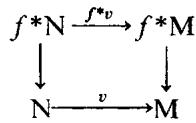
\includegraphics[keepaspectratio]{images/part001_e53c46a7.jpg}}

交换。

7.2.5. 设 B' 是 B 的子流形，i 是从 B' 到 B 的典范嵌入。若 M 是以 B 为基底的向量丛，则 \(i^*M\) 称为 M 在 B' 上诱导的向量丛，记为 \(M|_{B'}\)。若 \(t = (\mathrm{U}, \varphi, \mathrm{F})\) 是 M 的一个向量丛图，则 \((\mathrm{U} \cap \mathrm{B}', \varphi | \pi^{-1}(\mathrm{U} \cap \mathrm{B}'), \mathrm{F})\) 是 \(M|_{B'}\) 的一个向量丛图。从 \(M|_{B'}\) 到 M 的典范 f-态射是从 \(M|_{B'}\) 到 M 的子流形 \(\pi^{-1}(\mathrm{B}')\) 的一个流形同构。

7.2.6. 设 \(f\) 是从流形 B' 到 B 的态射，M（分别 M'）是以 B（分别 B'）为基底的向量丛。从 M 到 M' 的 \(f\)-余态射定义为从 \(f^{*}M\) 到 M' 的 B'-态射。当 B = B' 且 \(f = \mathrm{Id}_{\mathbf{B}}\) 时，从 M 到 M' 的 f-余态射的数据等价于从 M 到 M' 的 B-态射的数据。

设 \(g\) 是一个 \(f\)-余态射，从 \(\mathbf{M}\) 到 \(\mathbf{M}'\)。对每个 \(b \in \mathbf{B}'\)，映射 \(g_b: x \mapsto g(b, x)\) 从 \(\mathbf{M}_{f(b)}\) 到 \(\mathbf{M}_b'\)，是连续线性映射。

此外，设 \(f'\) 是从流形 \(B''\) 到 \(B'\) 的态射，且 \(h\) 是一个 \(f'\)-余态射，从 \(M'\) 到向量丛 \(M''\)，其基底为 \(B''\)。于是，映射 \(h \circ f'^{*}g\)，其定义域为 \(f'^{*}(f^{*}M) = (f \circ f')^{*}M\)，值域为 \(M''\)，是 \((f \circ f')\)-余态射，从 \(M\) 到 \(M''\)，记为 \(h \circ g\)。对于 \(b \in B''\)，有

\[
(h \circ g) _ {b} = h _ {b} \circ g _ {f ^ {\prime} (b)}.
\]

\subsection{多线性态射}

7.3.1. 设 \(M_{1},\ldots,M_{d}\) 和 N 是以 B 为基底的向量丛，u 是从集合 \(M_{1}\times_{B}\ldots\times_{B}M_{d}\) 到 N 的映射。如果满足以下条件，则称 u 为多线性态射（或 d-线性态射）：

对于每个 \(b_0 \in \mathbf{B}\)，存在一个开邻域 \(\mathbf{U}\)，包含 \(b_0\) 且位于 \(\mathbf{B}\) 中，存在向量丛图 \(t^j = (\mathbf{U}, \varphi^j, \mathbf{F}^j)\)，它们属于 \(\mathbf{M}_j\)（\(1 \leqslant j \leqslant d\)），以及向量丛图 \(t = (\mathbf{U}, \varphi, \mathbf{F})\)，它属于 \(\mathbf{N}\)，还有映射 \(\lambda\)，其类为 \(\mathbf{C}^r\)，从 \(\mathbf{U}\) 到巴拿赫空间 \(\mathcal{L}(\mathbf{F}^1, \ldots, \mathbf{F}^d; \mathbf{F})\)，该空间由从 \(\mathbf{F}^1 \times \cdots \times \mathbf{F}^d\) 到 \(\mathbf{F}\) 的连续 d-线性映射组成，使得：

\[
(t _ {b} \circ \lambda (b)) (x _ {1}, \dots , x _ {d}) = u (t _ {b} ^ {1} (x _ {1}), \dots , t _ {b} ^ {d} (x _ {d}))
\]

对所有 \(b \in \mathbf{U}\) 和所有 \(x_{j} \in \mathbf{F}^{j}\) 都成立。

每个多线性态射 \(u\) 都是从纤维积 \(\mathbf{M}_{1} \times_{\mathbf{B}} \cdots \times_{\mathbf{B}} \mathbf{M}_{d}\) 到 \(\mathbf{N}\) 的流形态射，并且对每个 \(b \in \mathbf{B}\) 诱导出一个连续 \(d\)-线性映射 \(u_b\)，从 \((\mathbf{M}_{1})_{b} \times \cdots \times (\mathbf{M}_{d})_{b}\) 到 \(\mathbf{N}_{b}\)。

若 \(f\) 是从 B 到流形 \(\mathbf{B}'\) 的态射，则从 \(\mathbf{M}_1 \times_{\mathbf{B}} \cdots \times_{\mathbf{B}} \mathbf{M}_d\) 到向量丛 \(\mathbf{M}'\)（其基底为 \(\mathbf{B}'\)）的多线性态射，按定义是从 \(\mathbf{M}_1 \times_{\mathbf{B}} \cdots \times_{\mathbf{B}} \mathbf{M}_d\) 到 \(f^*\mathbf{M}'\) 的多线性态射与由 \(f\) 给出的从 \(f^*\mathbf{M}'\) 到 \(\mathbf{M}'\) 的典范态射的复合。

双线性态射也称为配对。当 \(d=1\) 时，线性态射就是 7.2.1 意义下的态射。当 \(d=0\) 时，0-线性态射与 N 的一个截面（7.4）等同。

7.3.2. 以 B 为基底的代数丛是以 B 为基底、配备了从 \(A \times_{B} A\) 到 A 的配对的向量丛 A。于是每个纤维 \(A_{b}\) 都带有一个 K-代数结构。若对每个 \(b \in B\)，代数 \(A_{b}\) 有单位元，记为 \(e_{b}\)，则映射 \(b \mapsto e_{b}\) 是 A 的一个截面（参见 7.4）。如果对 B 中每个点 \(b_{0}\)，都存在一个向量丛图 \(t = (\mathrm{U}, \varphi, \mathrm{E})\)，它属于 A 并在点 \(b_{0}\) 处，以及 E 上的 K-代数结构，使得 \(t_{b}\) 是从 E 到 \(A_{b}\) 的代数同构，对所有 \(b \in U\) 均如此，则称代数丛 A 是局部平凡的。

7.3.3. 设 A 是以 B 为基底的带单位元的结合代数丛。以 B 为基底的 A-模丛定义为以 B 为基底的向量丛 M，配备一个配对 \(m: A \times_{B} M \to M\)，使得映射 \(m_{b}: A_{b} \times M_{b} \to M_{b}\) 对每个 \(b \in B\) 定义出 \(A_{b}\) 在纤维 \(M_{b}\) 上的模结构。

设 M 和 M′ 是两个 A-模向量丛。从 M 到 M′ 的 A-同态定义为以 B 为基底的向量丛态射 \(g: M \rightarrow M'\)，它对 B 中每个 b 都诱导出一个 \(A_b\)-线性映射，从 \(M_b\) 到 \(M_b'\)。

设 A 是局部平凡的。若对 B 中每个点 \(b_0\)，都存在一个向量丛图 \(t = (U, \varphi, E)\)，它是如 7.3.2 中所述的 A 在 \(b_0\) 处的图；另有一个向量丛图 \(t' = (U, \varphi', L)\)，它是 M 在 \(b_0\) 处的图；以及 L 上的 E-模结构，使得对每个 \(b \in U\)，\(t_b'\) 是 \(t_b\)-同构，将 \(A_b\)-模 \(M_b\) 映到 E-模 L，则称 A-模丛 M 是局部平凡的。

7.3.4. 设 A 是 K 上的巴拿赫代数（例如，带有有限维 K-代数结构的域）。平凡丛 \(A_{B}\) 于是是一个局部平凡代数丛。A-模 \(A_{B}\) 中的局部平凡丛 M 也称为 A 上的向量丛（以 B 为基底）。于是纤维 \(M_{b}\) 是拓扑 A-模。从 M 到另一个 A 上的向量丛的 f-态射 u 称为 A-线性的，如果映射 \(u_{b}\) 对所有 \(b \in B\) 都是 A-线性的。

\subsection{截面}

7.4.1. 设 M 是以 B 为基底的向量丛。对 B 的每个开集 U，记 \(\mathcal{S}_{\mathbf{M}}^{r}(\mathbf{U})\) 为 M 在 U 上的类为 \(C^r\) 的截面集，即从 U 到 M 的态射 \(s\)，其类为 \(C^r\)，满足 \(s(b) \in M_b\) 对所有 \(b \in \mathbf{U}\) 都成立。根据以下规则，这个集合带有关于态射函数环 \(\mathcal{C}^r(\mathbf{U})\) 的模结构：

\begin{enumerate}
\def\labelenumi{(\arabic{enumi})}
\tightlist
\item
\end{enumerate}

\[
(s + s ^ {\prime}) (b) = s (b) + s ^ {\prime} (b)\tag{2}
\]

\[
(\varphi . s) (b) = \varphi (b). s (b)
\]

其中 \(s, s'\) 属于 \(\mathcal{S}_{\mathrm{M}}^{r}(\mathrm{U})\)，\(\varphi\) 属于 \(\mathcal{C}^{r}(\mathrm{U})\)。当开集 U 变化时，得到一个从 B 到 M 的映射层 \(\mathcal{S}_{\mathrm{M}}^{r}\)（参见第 5.4.1 号），称为 M 的截面层。

7.4.2. 设 \(M_{1},\ldots,M_{d}\) 和 N 是以 B 为基底的向量丛，u 是从 \(M_{1}\times_{B}\ldots\times_{B}M_{d}\) 到 N 的多线性态射。对 \(1\leqslant j\leqslant d\)，给定一个截面 \(s_{j}\)，它是 \(M_{j}\) 在 B 的一个开集 U 上的截面；按下式在 U 上定义 N 的截面 \(u(s_{1},\ldots,s_{d})\)：

\[
u (s _ {1}, \dots , s _ {d}) (b) = u _ {b} (s _ {1} (b), \dots , s _ {d} (b)) \quad \text {   for   } b \in \mathrm{U}.
\]

映射 \((s_1, \ldots, s_d) \mapsto u(s_1, \ldots, s_d)\) 是 \(\mathcal{C}^r(\mathrm{U})\)-多线性的，有时记为 \(\mathcal{S}(u)\)。

7.4.3. 设 \(f\) 是从流形 \(\mathbf{B}'\) 到 \(\mathbf{B}\) 的态射，\(\mathbf{M}\) 是以 \(\mathbf{B}\) 为基底的向量丛。对每个开集 \(\mathbf{U}\)，它属于 \(\mathbf{B}\)，以及每个 \(s \in \mathcal{S}_{\mathbf{M}}^{r}(\mathbf{U})\)，映射 \(x \mapsto (x, s(f(x)))\) 是类为 \(\mathbf{C}^r\) 的 \(f^{*}\mathbf{M}\) 在开子集 \(f^{-1}(\mathbf{U})\) 上的截面，记为 \(f^{*}s\)，称为 \(s\) 关于 \(f\) 的逆像。映射 \(s \mapsto f^{*}s\) 从 \(\mathcal{S}_{\mathbf{M}}^{r}(\mathbf{U})\) 到 \(\mathcal{S}_{f^{*}\mathbf{M}}^{r}(f^{-1}(\mathbf{U}))\) 关于同态 \(g \mapsto g \circ (f|f^{-1}(\mathbf{U}))\)（它从 \(\mathcal{C}^{r}(\mathbf{U})\) 到 \(\mathcal{C}^{r}(f^{-1}(\mathbf{U}))\)）是半线性的。

此外，若 N 是以 B' 为基底的向量丛，g 是从 M 到 N 的 f-余态射，有时将记为 \(\mathcal{S}(g)\) 的映射 \(s \mapsto g \circ f^{*}s\) 从 \(\mathcal{S}_{\mathbf{M}}^{\mathbf{r}}(\mathbf{U})\) 到 \(\mathcal{S}_{\mathbf{N}}^{\mathbf{r}}(f^{-1}(\mathbf{U}))\)。

7.4.4. 设 M 是以 B 为基底的有限秩向量丛。M 在 B 的一个开集 U 上的标架定义为 M 在 U 上的截面组成的有限序列 \((s_{1},\ldots,s_{n})\)，使得 \((s_{1}(b),\ldots,s_{n}(b))\) 是向量空间 \(M_{b}\) 的一个基，对所有 \(b\in U\) 均如此。于是序列 \((s_{1},\ldots,s_{n})\) 是 \(\mathcal{C}^{r}(\mathrm{U})\)-模 \(\mathcal{S}_{\mathbf{M}}^{r}(\mathrm{U})\) 的一个基。若 f 是从流形 \(B'\) 到 B 的态射，则截面 \(f^{*}s_{j}\) 构成 \(f^{*}\mathbf{M}\) 在 \(f^{-1}(\mathbf{U})\) 上的一个标架。

7.4.5. 设 L 是一个赋有有限维 K-代数结构的域，(M, B, π) 是一个纤维化。假定每个纤维 \(M_{b}\) 上都给定了有限维的 L-向量空间结构。M 上至多存在一个以 B 为基底的向量丛结构，它与映射 π、M 的流形结构以及各纤维上的 L-向量空间结构相容（7.3.4）。这种结构存在的充要条件是满足以下条件：

（FV）对每个 \(b_0 \in \mathbf{B}\)，存在一个开邻域 \(\mathbf{U}\)，其中包含 \(b_0\) 且位于 \(\mathbf{B}\) 中，以及一个流形同构 \(\varphi\)，它从 \(\pi^{-1}(\mathbf{U})\) 到乘积 \(\mathbf{U} \times \mathbf{F}\)，它是 \(\mathbf{U}\) 与 \(\mathbf{F}\) 的乘积，其中后者是有限维的 \(\mathbf{L}\)-向量空间，使得对每个 \(b \in \mathbf{U}\)，双射 \(\varphi_b\) 从 \(\mathbf{M}_b\) 到 \(\mathbf{F}\) 由 \(\varphi\) 诱导，并且是 \(\mathbf{L}\) 上的向量空间同构。

于是，满足（FV）的三元组（U，\(\varphi\)，F）就是向量丛 M 的向量丛图。

条件（FV）等价于：

（FV'）对每个 \(b_0 \in \mathbf{B}\)，存在一个整数 \(n\) 以及 \(n\) 个截面 \(s_1, \ldots, s_n\)，它们是 \(\mathbf{M}\) 在开邻域 \(\mathbf{U}\) 上的截面，而该邻域包含 \(b_0\)，使得映射

\[
(b, a _ {1}, \dots , a _ {n}) \mapsto a _ {1} s _ {1} (b) + \dots + a _ {n} s _ {n} (b)
\]

是从流形 \(\mathbf{U} \times \mathbf{L}^{n}\) 到流形 \(\pi^{-1}(\mathbf{U})\) 的同构。

7.4.6. 设 \(M_{1},\ldots,M_{d}\) 和 N 是以 B 为基底的向量丛，其中 \(M_{j}\) 为有限秩。假定对 B 的每个开集 U，都给定了一个 \(\mathcal{C}^{r}(\mathrm{U})\)-多线性映射 \(\varphi_{\mathrm{U}}\)，从 \(\mathcal{S}_{\mathrm{M}_{1}}^{\mathrm{r}}(\mathrm{U})\times\cdots\times\mathcal{S}_{\mathrm{M}_{d}}^{\mathrm{r}}(\mathrm{U})\) 到 \(\mathcal{S}_{\mathrm{N}}^{\mathrm{r}}(\mathrm{U})\)，使得当 \(V \subset U\) 时有：

\[
\varphi_ {\mathrm{U}} (s _ {1}, \dots , s _ {d}) | \mathrm{V} = \varphi_ {\mathrm{V}} (s _ {1} | \mathrm{V}, \dots , s _ {d} | \mathrm{V}).
\]

于是存在一个多线性态射 \(u\)，从 \(\mathbf{M}_1 \times_{\mathbf{B}} \ldots \times_{\mathbf{B}} \mathbf{M}_d\) 到 \(\mathbf{N}\)，使得 \(\varphi_{\mathbf{U}}(s_1, \ldots, s_d) = u(s_1, \ldots, s_d)\) 对任意截面 \(s_j\)，属于 \(\mathbf{M}_j\) 在开集 \(\mathbf{U}\)（属于 \(\mathbf{B}\)）上的截面，均成立。

7.4.7. 设 \(f\) 是从流形 \(\mathbf{B}'\) 到 \(\mathbf{B}\) 的态射，且 \(\mathbf{M}\)（分别 \(\mathbf{M}'\)）是以 \(\mathbf{B}\)（分别 \(\mathbf{B}'\)）为基底的有限秩向量丛。假定对每个开集 \(\mathbf{U}\)，它属于 \(\mathbf{B}\)，给定一个连续的 \(\mathcal{C}^{r}(\mathbf{U})\)-半线性映射 \(\varphi_{\mathbf{U}}\)，从 \(\mathcal{S}_{\mathbf{M}}^{r}(\mathbf{U})\) 到 \(\mathcal{S}_{\mathbf{M}'}^{r}(f^{-1}(\mathbf{U}))\)，使得

\[
\varphi_ {\mathbf {U}} (s) | f ^ {- 1} (\mathbf {V}) = \varphi_ {\mathbf {V}} (s | \mathbf {V})
\]

对每个开集 \(V \subset U\) 都有。于是存在唯一一个从 M 到 \(M'\) 的 f-余态射 g，使得 \(\varphi_{\mathrm{U}}(s) = \mathcal{S}(g)(s)\) 对所有 \(s \in \mathcal{S}_{\mathrm{M}}^{r}(\mathrm{U})\) 都成立。

*7.4.8. 设 \(\mathcal{F}\) 是关于环层 \(\mathcal{C}_{\mathrm{B}}^{r}\) 的模层。我们称 \(\mathcal{F}\) 是局部自由的：对每个 \(b \in \mathrm{B}\)，存在一个开邻域 U，含有 \(b\)，以及一个整数 \(n\)，使得 \(\mathcal{F}|\mathrm{U}\) 与一个 \(\mathcal{C}_{\mathrm{U}}^{r}\)-模层 \((\mathcal{C}_{\mathrm{U}}^{r})^{n}\) 同构。

若 M 是以 B 为基底的有限秩向量丛，则层 \(\mathcal{S}_{\mathrm{M}}^{r}\) 是局部自由的。反之，对 B 上每个局部自由层 \(\mathcal{F}\)，存在一个向量丛 M 以及从 \(\mathcal{S}_{\mathrm{M}}^{r}\) 到 \(\mathcal{F}\) 的层同构。若 M' 是另一个以 B 为基底的有限秩向量丛，则映射 \(g \mapsto \mathcal{S}(g)\) 是从 M 到 M' 的 B-态射集到从 \(\mathcal{C}^{r}\)-模层态射 \(\mathcal{S}_{\mathrm{M}}^{r}\) 到 \(\mathcal{S}_{\mathrm{M}'}^{r}\) 的集合的双射。

\subsection{子向量丛、商向量丛、正合序列}

本号中，向量丛均指以 B 为基底的向量丛，向量丛态射均指 \(\mathrm{Id}_{\mathbf{B}}\)-态射。

7.5.1. 设 M 是一个向量丛。如果对每个点 \(b \in B\)，都存在 M 在 b 处的向量丛图 \(t = (\mathbf{U}, \varphi, \mathbf{E})\) 以及 E 的一个具有拓扑补空间的闭向量子空间 F，使得

\[
\varphi (\pi^ {- 1} (\mathrm{U}) \cap \mathrm{M} ^ {\prime}) = \mathrm{U} \times \mathrm{F}.
\]

在这些条件下，M′ 上存在唯一一个向量丛结构，使得从 M′ 到 M 的典范嵌入是一个态射。对每个 \(b \in B\)，M' 的纤维 \(M_{b}'\) 是闭向量子空间 \(M' \cap M_{b}\)，并且该空间包含于 \(M_{b}\)；M' 是 M 的闭子流形，并且 M' 的向量丛结构的底层流形结构与由 M 的流形结构诱导的结构一致。

7.5.2. 设 M' 是 M 的一个子向量丛。用 R 表示 M 的点 x、y 之间的如下关系：

存在 \(b\) 属于 \(B\)，使得 \(x \in M_b, y \in M_b\) 且 \(x - y \in M_b'\)。于是 \(R\) 是 \(M\) 上的正则等价关系（参见第 5.9.7 号）。集合 \(M/R\) 上存在唯一一个向量丛结构，使得从 \(M\) 到 \(M/R\) 的典范映射是一个态射。将其记为 \(M/M'\)，并称 \(M\) 对 \(M'\) 的商为如此定义的向量丛；对于 \(b\) 属于 \(B\) 的每个点，丛 \((M/M')_b\) 是商拓扑向量空间 \(M_b/M_b'\)，而 \(M/M'\) 上的流形结构是 \(M\) 上流形结构的商结构。

7.5.3. 保留 7.5.2 的假设。对于 B 的每个点 \(b_0\)，可以找到一个开邻域 U，其中包含 \(b_0\)；一个巴拿赫空间 F，它是两个闭子空间 \(F'\) 和 \(F''\) 的直和；以及一个向量丛同构 \(\iota\)，从 \(\mathbf{F}_{\mathbf{U}}\) 到 \(\mathbf{M}|\mathbf{U}\)，满足以下性质：

\begin{enumerate}
\def\labelenumi{(\roman{enumi})}
\item
  \(\iota'\) 是 \(\iota\) 在 \(\mathbf{U} \times \mathbf{F}'\) 上的限制，并且是从 \(\mathbf{F}_{\mathbf{U}}'\) 到 \(\mathbf{M}'|\mathbf{U}\) 的同构。
\item
  若 \(\rho\) 是从 M 到 \(\mathbf{M}'' = \mathbf{M} / \mathbf{M}'\) 的典范映射，且 \(\iota''\) 是 \(\iota\) 在 \(\mathbf{U} \times \mathbf{F}''\) 上的限制，则映射 \(\rho \circ \iota''\) 是从 \(\mathbf{F}_{\mathbf{U}}''\) 到 \(\mathbf{M}''|\mathbf{U}\) 的同构。
\end{enumerate}

7.5.4. 若向量丛态射 \(g: \mathbf{L} \to \mathbf{M}\) 的像包含于 \(\mathbf{M}'\)，则它是从 \(\mathbf{L}\) 到 \(\mathbf{M}'\) 的向量丛态射。

现在设 \(h: \mathbf{M} \to \mathbf{N}\) 是一个向量丛态射，并假定对 B 中的每个 \(b\)，\(h_b\) 在 \(\mathbf{M}_b'\) 上的限制为零。若 \(\rho\) 是从 M 到 \(\mathbf{M}/\mathbf{M}'\) 的典范态射，则存在唯一一个态射 \(\bar{h}\)，其从 \(\mathbf{M}/\mathbf{M}'\) 到 N，且满足 \(h = \bar{h} \circ \rho\)。

7.5.5. 设 P、Q 是两个向量丛，g 是从 P 到 Q 的态射；对 B 中的每个点 b，分别以 \(N_{b}\) 和 \(I_{b}\) 表示线性映射 \(g_{b}:P_{b}\to Q_{b}\) 的核和像。置 \(N=\bigcup_{b\in B}N_{b}\)，以及

\(I = \bigcup_{b \in B} I_b\)。称态射 \(g\) 是局部直的，当且仅当 \(N\) 是 P 的子向量丛且 I 是 Q 的子向量丛。于是态射 g 通过取商定义了从 P/N 到 I 的同构。称 N 为 g 的核，记为 Ker g。同样，子丛 I 称为 g 的像，记为 Im g。

若 \(r \geqslant \infty\)，则态射 \(g\) 局部直当且仅当 \(g\) 是子浸入。若 P 是有限秩的，则态射 \(g\) 局部直当且仅当 \(g\) 的向量秩局部常值，或者等价地，当且仅当 \(g\) 是子浸入。

7.5.6. 设 \(\mathbf{M} \xrightarrow{f} \mathbf{M}' \xrightarrow{g} \mathbf{M}''\) 是两个向量丛态射。称序列 \((f, g)\) 是局部直正合的，当且仅当 \(f\) 和 \(g\) 都局部直且 \(\operatorname{Im} f = \operatorname{Ker} g\)。若 \(g \circ f = 0\)，令 \(\mathbf{D}\) 为满足以下条件的点 \(b \in \mathbf{B}\) 的集合：序列 \(\mathbf{M}_b \xrightarrow{f_b} \mathbf{M}_b' \xrightarrow{g_b} \mathbf{M}_b''\) 是直正合的（即 \(\operatorname{Ker} f_b\) 和 \(\operatorname{Im} g_b\) 有拓扑补空间，且 \(\operatorname{Im} f_b = \operatorname{Ker} g_b\)）。则 D 是开集，并且序列 \(\mathbf{M}|\mathbf{D} \xrightarrow{f} \mathbf{M}'|\mathbf{D} \xrightarrow{g} \mathbf{M}''|\mathbf{D}\) 是局部直正合的。

任意长度的局部直正合序列也以同样方式定义。语言上滥用时，有时用“直正合序列”代替“局部直正合序列”。

7.5.7. 设 \(0 \to \mathbf{M} \xrightarrow{f} \mathbf{M}' \xrightarrow{g} \mathbf{M}'' \to 0\) 是一个向量丛态射序列。这个序列局部直正合的充要条件是：\(f\) 是从 \(\mathbf{M}\) 到子向量丛 \(f(\mathbf{M})\) 的同构，该子丛属于 \(\mathbf{M}'\)，并且 \(g\) 通过取商定义了从商向量丛 \(\mathbf{M}'/f(\mathbf{M})\) 到 \(\mathbf{M}''\) 的同构。

\subsection{向量函子}

本号以及其后的三个 7.7 至 7.9 号中，字母 I 表示一个有限集，它是两个不交子集 \(I_+\) 和 \(I_-\) 的并。我们用 \(\mathcal{V} = (\mathrm{V}_{i})_{i\in I}\)（\(\mathcal{V}'\)、\(\mathcal{V}''\)、\ldots）也同样表示一个由 I 编号的巴拿赫空间族。我们用 \(\operatorname{Hom}(\mathcal{V},\mathcal{V}')\) 表示巴拿赫空间 \(\prod_{i\in I_+}\mathcal{L}(\mathrm{V}_i;\mathrm{V}_i')\times \prod_{i\in I_-}\mathcal{L}(\mathrm{V}_i';\mathrm{V}_i)\)。我们用 \(\mathbf{f} = (f_i)\) 表示 \(\operatorname{Hom}(\mathcal{V},\mathcal{V}')\) 的一个元素。将 \(\mathrm{Id}_{\mathcal{V}}\) 记为元素 \((\mathrm{Id}_{\mathrm{V}_i})_{i\in I}\)，它属于 \(\operatorname{Hom}(\mathcal{V},\mathcal{V})\)。对于 \(\mathbf{f}\in \operatorname{Hom}(\mathcal{V},\mathcal{V}')\) 和 \(\mathbf{f}'\in \operatorname{Hom}(\mathcal{V}',\mathcal{V}'')\)，用 \(\mathbf{f}'\circ \mathbf{f}\) 表示 \(\operatorname{Hom}(\mathcal{V},\mathcal{V}'')\) 中的元素，其分量由下式给出：

\[
\begin{array}{l l} (\mathbf {f} ^ {\prime} \circ \mathbf {f}) _ {i} = f _ {i} ^ {\prime} \circ f _ {i} & \text { if } \quad i \in \mathrm{I} _ {+} \\ (\mathbf {f} ^ {\prime} \circ \mathbf {f}) _ {i} = f _ {i} \circ f _ {i} ^ {\prime} & \text { if } \quad i \in \mathrm{I} _ {-}. \end{array}
\]

7.6.1. 类型为 I 且类为 \(\mathbf{C}^r\) 的向量函子（分别为有限维向量函子）是由如下数据组成的：对于每个由巴拿赫空间（分别为 K 上的有限维向量空间）组成的族 \(\mathcal{V} = (\mathrm{V}_i)_{i\in I}\)，给定一个巴拿赫空间 \(\tau(\mathcal{V})\)；对于每个 \(\mathbf{f}\in\mathrm{Hom}(\mathcal{V},\mathcal{V}')\)，给定一个元素 \(\tau(\mathbf{f})\in\mathcal{L}(\tau(\mathcal{V});\tau(\mathcal{V}'))\)；这些数据满足以下两个条件：

\begin{enumerate}
\def\labelenumi{(\alph{enumi})}
\item
  有 \(\tau (\mathrm{Id}_{\mathcal{V}}) = \mathrm{Id}_{\tau (\mathcal{V})}\)，且 \(\tau (\mathbf{f}'\circ \mathbf{f}) = \tau (\mathbf{f}')\circ \tau (\mathbf{f}).\)
\item
  映射 \(\tau : \operatorname{Hom}(\mathcal{V}, \mathcal{V}') \to \mathcal{L}(\tau(\mathcal{V}); \tau(\mathcal{V}'))\) 的类为 \(C'\)。
\end{enumerate}

7.6.2. 设 \(\mathcal{M} = (\mathbf{M}^i)_{i\in I}\) 是以 B 为基底的向量丛族。对 \(b\in \mathbf{B}\)，置 \(\mathcal{M}_b = (\mathbf{M}_b^i)_{i\in I}\)。设 \(\tau\) 是一个向量函子，并用 \(\tau (\mathcal{M})\) 表示所有 \(\tau(\mathcal{M}_{b})\) 的不交并，其中 \(b\in\mathbf{B}\)。

在 \(\tau(\mathcal{M})\) 上存在唯一一个向量丛结构（以 B 为基底，相对于映射 \(\pi\)，该映射从 \(\tau(\mathcal{M})\) 到 B），使得对每个 \(b\in\mathbf{B}\)，都有 \(\tau(\mathcal{M}_{b})=\pi^{-1}(b)\)，并且具有以下性质：

设 U 是 B 的一个开子集，并且对每个 i，设 \(t^{i} = (\mathrm{U}, \varphi_{i}, \mathrm{F}_{i})\) 是定义域为 U 的 \(M^{i}\) 的向量丛图；置 \(\mathcal{F} = (\mathrm{F}_{i})_{i \in I}\)，并令 \(\psi_{b}\) 为 \(\operatorname{Hom}(\mathcal{M}_{b}, \mathcal{F})\) 中的元素，满足 \((\psi_{b})_{i} = (t_{b}^{i})^{-1}\) 对 \(i \in I_{+}\) 成立，且 \((\psi_{b})_{i} = t_{b}^{i}\) 对 \(i \in I_{-}\) 成立；对 \(x \in \pi^{-1}(\mathrm{U})\)，置 \(\psi(x) = (\pi(x), \tau(\psi_{\pi(x)})(x))\)。则三元组 \((\mathrm{U}, \psi, \tau(\mathcal{F}))\) 是向量丛 \(\tau(\mathcal{M})\) 的一个向量丛图。

赋予这个结构后，\(\tau(\mathcal{M})\) 称为由向量丛族 \(\mathcal{M}\) 通过向量函子 \(\tau\) 导出的向量丛。

7.6.3. 设 \(f\) 是从 \(\mathbf{B}\) 到流形 \(\mathbf{B}'\) 的态射。设 \(\mathcal{M} = (\mathbf{M}^i)\)（分别 \(\mathcal{M}' = (\mathbf{M}'^i)\)）是由 \(\mathbf{I}\) 编号的、以 \(\mathbf{B}\)（分别 \(\mathbf{B}'\)）为基底的向量丛族。对每个 \(i \in \mathbf{I}_+\)，设 \(g_i\) 是一个 \(f\)-态射，从 \(\mathbf{M}^i\) 到 \(\mathbf{M}'^i\)；对每个 \(i \in \mathbf{I}_-\)，设 \(g_i\) 是一个 \(f\)-余态射，从 \(\mathbf{M}'^i\) 到 \(\mathbf{M}^i\)。置 \(\mathbf{g} = (g_i)_{i \in I}\)，并对 \(b \in B\) 置 \(\mathbf{g}_b = ((g_i)_b)_{i \in I}\)（参见 7.2.1 和 7.2.6）。存在一个 \(f\)-态射，记为 \(\tau(\mathbf{g})\)，从 \(\tau(\mathcal{M})\) 到 \(\tau(\mathcal{M}')\)，且唯一，使得 \(\tau(\mathbf{g})_b = \tau(\mathbf{g}_b)\) 对所有 \(b \in B\) 都成立。

特别地，若 \(M^{i}=f^{*}M^{'i}\)，且 \(g_{i}\) 是典范态射或余态射，则从 \(\tau(\mathcal{M})\) 到 \(f^{*}\tau(\mathcal{M}')\) 的 B-态射由 \(\tau(\mathbf{g})\)（7.2.4）定义，是一个同构；这个事实表述为 \(\tau\) 与逆像可交换。

特别地，设 B' 是 B 的子流形，并置 \(\mathcal{M}|B' = (M^{i}|B')_{i\in I}\)。则向量丛 \(\tau(\mathcal{M})|B'\) 与 \(\tau(\mathcal{M}|B')\) 典范地 B'-同构。

7.6.4. 设 \(\tau, \tau_1, \ldots, \tau_d\) 是向量函子（类型为 I 且类为 \(C'\)）。一个 \(d\)-线性态射 \(\theta\)，从 \((\tau_1, \ldots, \tau_d)\) 到 \(\tau\)，是如下数据：对于每个由 I 编号的巴拿赫空间族 \(\mathcal{V}\)，给定一个连续 \(d\)-线性映射 \(\theta_{\mathcal{V}}\)，从 \(\tau_1(\mathcal{V}) \times \cdots \times \tau_d(\mathcal{V})\) 到 \(\tau(\mathcal{V})\)，这些数据满足以下条件：对每个 \(f \in \text{Hom}(\mathcal{V}, \mathcal{V}')\)，有

\[
\tau (\mathbf {f}) \circ \theta_ {\mathcal{V}} = \theta_ {\mathcal{V}^{\prime}} \circ (\tau_ {1} (\mathbf {f}) \times \dots \times \tau _{d} (\mathbf {f})).
\]

当 \(d = 1\) 时，简称为从 \(\tau_1\) 到 \(\tau\) 的态射。

现在设 \(\mathcal{M}\) 是由 I 编号的、以 B 为基底的向量丛族。存在唯一一个 B-态射 \(\theta_{\mathcal{M}}\)，从 \(\tau_{1}(\mathcal{M}) \times_{\mathbf{B}} \cdots \times_{\mathbf{B}} \tau_{d}(\mathcal{M})\) 到 \(\tau(\mathcal{M})\)，它是 d-线性的，并且满足 \((\theta_{\mathcal{M}})_{b} = \theta_{\mathcal{M}_{b}}\) 对所有 \(b \in \mathbf{B}\) 都成立。

采用 7.6.3 的记号，有

\[
\tau (\mathbf {g}) \circ \theta_ {\mathcal {M}} = \theta_ {\mathcal {M} ^ {\prime}} \circ (\tau_ {1} (\mathbf {g}) \times \dots \times \tau_ {d} (\mathbf {g})).
\]

若 \(d=1\) 且 \(\theta\) 是同构（即 \(\theta_{\mathcal{V}}\) 对每个族 \(\mathcal{V}\) 都是同构），则 \(\theta_{\mathcal{M}}\) 是同构。

7.6.5. 7.6.2 至 7.6.4 号的定义和结果可推广到有限维向量函子的情形，条件是处处假定所给向量丛为有限秩。

它们也可推广到如下情形：设 L 是带有有限维 K-代数结构的域；取 \(\tau\) 为 L 上的向量函子（即满足将 7.6.1 中的 K 换成 L 后所得假设的函子），并且只考虑 7.3.4 意义下 L 上的向量丛。

7.6.6. 如果一个函子对每个巴拿赫空间 V（分别每个 K 上的有限维向量空间）赋予一个巴拿赫空间 \(\tau(\mathrm{V})\)，并对从 V 到巴拿赫空间 V' 的每个同构 \(f\) 赋予一个同构 \(\tau(f)\)，其从 \(\tau(\mathrm{V})\) 到 \(\tau(\mathrm{V}')\)，且这些数据满足 7.6.1 的条件（a）和以下条件，则称该函子是关于同构的向量函子（分别有限维向量函子）：

（b'）映射 \(f\mapsto\tau(f)\) 从由 V 到 V' 的同构组成的 \(\mathcal{L}(\mathrm{V};\mathrm{V}')\) 的开子集到 \(\mathcal{L}(\tau(\mathrm{V});\tau(\mathrm{V}'))\) 是 C' 类的。

前面各号的定义和结果可推广到关于同构的向量函子的情形（令 \(I_{+} = \{1\}\) 且 \(I_{-} = \varnothing\)），但 7.6.3 号第一段中的定义和结果除外。

\subsection{直和、多线性映射丛、对偶}

7.7.1. 假设 \(I_{-} = \emptyset\)。定义向量函子 \(\sigma\)，称为直和函子，规定 \(\sigma(\mathcal{V}) = \bigoplus_{i \in I} V_i\) 且 \(\sigma(f) = \bigoplus_{i \in I} f_i\)。若 \(\mathcal{M} = (M^i)_{i \in I}\) 是以 B 为基底的向量丛族，则向量丛 \(\sigma(\mathcal{M})\) 称为 \(M^i\) 的直和，记为 \(\bigoplus_{i \in I} M^i\)。对每个 \(b \in B\)，在 \(b\) 处的 \(\bigoplus_{i \in I} M^i\) 的纤维是各个 \(M^i\) 在 \(b\) 处的纤维的直和。设 U 是 B 的一个开子集，且 \(s_i \in \mathscr{S}_{M^i}^r(U)\)（\(i \in I\)）。则映射 \(b \mapsto \sum_{i \in I} s_i(b)\) 是一个截面，记为 \(\sum_{i} s_i\)，其类为 \(C^r\)，属于 \(M = \bigoplus_{i \in I} M^i\)；并且映射 \((s_i)_{i \in I} \mapsto \sum_{i} s_i\) 是一个 \(\mathscr{C}^r(U)\)-模同构，从 \(\bigoplus_{i} \mathscr{S}_{M^i}^r(U)\) 到 \(\mathscr{S}_M^r(U)\)。

\(\bigoplus_{i\in I}M^{i}\) 的底层流形与纤维积 \(\prod_{B}M^{i}\) 相同。

将 \(pr_{i}\) 记为从 \(\bigoplus_{i\in I} M^{i}\) 到 \(M^{i}\) 的向量丛态射；它在每个纤维 \(\bigoplus_{i\in I} M_{b}^{i}\) 上是第 i 个投影。类似地，定义典范嵌入 \(j_{i}\)，它将 \(M^{i}\) 嵌入 \(\bigoplus M^{i}\)。

设 \(f\) 是从 B 到流形 \(\mathbf{B}'\) 的态射；设 H 是另一个有限集，\(\mathcal{N} = (\mathrm{N}^{h})_{h\in \mathbf{H}}\) 是以 \(\mathbf{B}'\) 为基底的向量丛族。映射 \(u\mapsto \bigl(\mathrm{pr}_{h}\circ u\circ j_{i}\bigr)_{(h,i)\in \mathbf{H}\times \mathbf{I}}\) 是 \(f\)-态射集，从 \(\bigoplus_{i\in \mathbf{I}}\mathbf{M}^i\) 到 \(\bigoplus_{h\in \mathbf{H}}\mathbf{N}^h\)，到矩阵集 \((u_{h,i})_{(h,i)\in \mathbf{H}\times \mathbf{I}}\) 的双射，其中 \(u_{h,i}\) 是一个 \(f\)-态射，从 \(\mathbf{M}^i\) 到 \(\mathbf{N}^h\)。

若 I = \{1, 2\}，则序列

\[
0 \to \mathbf {M}^{1} \xrightarrow{j_{1}} \mathbf {M}^{1} \oplus \mathbf {M}^{2} \stackrel{\mathrm{pr}_{2}}{\to} \mathbf {M}^{2} \to 0
\]

是直正合的。

反之，设 M 是以 B 为基底的向量丛，M' 是 M 的子向量丛。假设流形 B 是仿紧的，且满足以下两个条件之一：

\begin{enumerate}
\def\labelenumi{(\roman{enumi})}
\item
  K 不同于 R 或 C；
\item
  \(\mathbf{K} = \mathbf{R}, r \neq \omega\)，且流形 \(\mathbf{B}\) 具有类为 \(C^r\) 的单位分解（5.3.6）。
\end{enumerate}

则存在 M 的一个子向量丛 M''，使得 M 可与直和 M' ⊕ M'' 认同。

7.7.2. 假设 \(I_{+}=\{0\}\) 且 \(I_{-}=\{1,2,\ldots,d\}\)。定义类型为 I 的向量函子 \(\eta_{d}\)，其类为 \(C^{r}\)，规定 \(\eta_{d}(\mathcal{V})=\mathcal{L}(V_{1},\ldots,V_{d};V_{0})\)，并规定 \(\eta_{d}(\mathbf{f})(u)=f_{0}\circ u\circ(f_{1}\times\cdots\times f_{d})\)，其中 \(u\in\eta_{d}(\mathcal{V})\)。若 \(\mathcal{M}=(M_{i})_{i\in I}\) 是以 B 为基底的向量丛族，则将向量丛 \(\eta_{d}(\mathcal{M})\) 记为 \(\mathcal{L}(M_{1},\ldots,M_{d};M_{0})\)。

设 \(u\) 是从 \(\mathbf{M}_{1} \times_{\mathbf{B}} \cdots \times_{\mathbf{B}} \mathbf{M}_{d}\) 到 \(\mathbf{M}_{0}\) 的多线性态射。映射 \(\hat{u}: b \mapsto u_{b}\) 于是是 \(\mathcal{L}(\mathbf{M}_{1}, \ldots, \mathbf{M}_{d}; \mathbf{M}_{0})\) 的一个截面，而映射 \(u \mapsto \hat{u}\) 是双射。

7.7.3. 保留 7.7.2 的记号，并进一步假设 \(d=1\)。向量丛 \(\mathcal{L}(\mathbf{M}_{1};\mathbf{M}_{0})\) 称为从 \(\mathbf{M}_{1}\) 到 \(\mathbf{M}_{0}\) 的同态丛。它的截面与从 \(\mathbf{M}_{1}\) 到 \(\mathbf{M}_{0}\) 的 B-态射相对应。

此外，若 \(M_{0}\) 是平凡丛 \(K_{B}\)，则向量丛 \(\mathcal{L}(\mathbf{M}_{1};\mathbf{K}_{\mathbf{B}})\) 称为 \(M = M_{1}\) 的对偶，记为 \(M'\)：纤维 \((\mathbf{M}')_{b}\) 是 M 的纤维 \(M_{b}\) 上的连续线性形式空间，其中点 \(b \in B\)。

若 \(s\)（分别 \(t\)）是 M（分别 M'）在 B 的一个开集 U 上的截面，则映射 \(b \mapsto (b, \langle s(b), t(b) \rangle)\) 是一个截面，记为 \(\langle s, t \rangle\)；这个截面属于平凡丛 \(\mathbf{K}_{\mathbf{B}}\)。¹

\subsection{交错多线性映射丛}

在 7.8.1 至 7.8.5 号中，我们假设 K 的特征为 0，或所考虑的向量丛具有有限秩。尚不知道 7.8.1 中给出的函子 \(\alpha_{d}\) 的定义是否可以不加任何限制地进行。

7.8.1. 取 \(\mathbf{I}_{+} = \{0\}\)、\(\mathbf{I}_{-} = \{1\}\)，并令 \(d\) 为满足 \(\geqslant 1\) 的整数。我们定义一个

\(^{1}\) 当 \(M\) 为有限秩时，我们用 \(M^{*}\) 代替 \(M'\)。

向量函子 \(\alpha_{d}\)：将 \(\alpha_{d}(\mathcal{V})\) 记为由连续交错 \(d\)-线性映射构成的巴拿赫空间，这些映射从 \(\mathbf{V}_{1}^{d}\) 到 \(\mathbf{V}_{0}\)，并规定 \(\alpha_{d}(\mathbf{f})(u) = f_{0} \circ u \circ f_{1}^{d}\)，其中 \(u \in \alpha_{d}(\mathcal{V})\)。将向量丛 \(\alpha_{d}((\mathbf{M}_{1}, \mathbf{M}_{0}))\) 记为 \(\operatorname{Alt}^{d}(\mathbf{M}_{1}; \mathbf{M}_{0})\)，称为交错 \(d\)-线性映射向量丛，从 \(\mathbf{M}_{1}\) 到 \(\mathbf{M}_{0}\)。

从 \(\operatorname{Alt}^{d}(\mathbf{M}_{1};\mathbf{M}_{0})\) 到 \(\mathcal{L}(\mathbf{M}_{1},\ldots,\mathbf{M}_{1};\mathbf{M}_{0})\) 的典范嵌入是向量丛态射；\(\operatorname{Alt}^{d}(\mathbf{M}_{1};\mathbf{M}_{0})\) 是 \(\mathcal{L}(\mathbf{M}_{1},\ldots,\mathbf{M}_{1};\mathbf{M}_{0})\) 的子向量丛。

有 \(\operatorname{Alt}^1 (\mathbf{M}_1;\mathbf{M}_0) = \mathcal{L}(\mathbf{M}_1;\mathbf{M}_0)\)。置 \(\operatorname{Alt}^0 (\mathbf{M}_1;\mathbf{M}_0) = \mathbf{M}_0\)。

若 \(\omega\) 是一个截面 \(^{1}\)，属于 \(\mathsf{Alt}^{d}(\mathbf{M}_{1};\mathbf{M}_{0})\)，且 \(s_{1},\ldots,s_{d}\) 是 \(\mathbf{M}_{1}\) 的截面，则存在唯一一个 \(\mathbf{M}_{0}\) 的截面，记为 \(\omega(s_{1},\ldots,s_{d})\)，使得

\[
\omega (s _ {1}, \dots , s _ {d}) (b) = \omega (b) (s _ {1} (b), \dots , s _ {d} (b)) \quad \text { for all } b \in \mathbf {B}.
\]

7.8.2. 设 \(\varphi\) 是从 \(N \times_{B} N'\) 到 \(N''\) 的配对（参见第 7.3.1 号）；对每个 \(b\)，有一个双线性映射 \(\varphi_b\)，从 \(N_b \times N_b'\) 到 \(N_b''\)，它定义了（参见附录 A，第 III 节，第 142 页）一个从

\[
\operatorname{Alt} ^ {d} (\mathbf {M}; \mathbf {N}) _ {b} \times \operatorname{Alt} ^ {e} (\mathbf {M}; \mathbf {N} ^ {\prime}) _ {b}
\]

到 \(\operatorname{Alt}^{d + e}(\mathbf{M};\mathbf{N}^{\prime \prime})_{b}\) 的双线性映射。这些双线性映射组成一个配对 \(u\)，从

\[
\operatorname{Alt} ^ {d} (\mathbf {M}; \mathbf {N}) \times_ {\mathbf {B}} \operatorname{Alt} ^ {e} (\mathbf {M}; \mathbf {N} ^ {\prime})
\]

到 \(\mathsf{Alt}^{d + e}(\mathbf{M};\mathbf{N}^{\prime \prime})\)；若 \(\omega\) 和 \(\omega^{\prime}\) 分别是 \(\mathsf{Alt}^{d}(\mathbf{M};\mathbf{N})\) 和 \(\mathsf{Alt}^{e}(\mathbf{M};\mathbf{N}^{\prime})\) 在开集 U 上的截面，则 \(u(\omega ,\omega^{\prime})\) 是 \(\mathsf{Alt}^{d + e}(\mathbf{M};\mathbf{N}^{\prime \prime})\) 在 U 上的截面，记为 \(\omega \wedge_{\varphi}\omega^{\prime}\)，称为 \(\omega\) 与 \(\omega^{\prime}\) 的外积。

有公式：

\[
(1) \quad \left(\omega \wedge_ {\varphi} \omega^ {\prime}\right) \left(s _ {1}, \dots , s _ {d + e}\right) = \sum_ {\sigma} \varepsilon_ {\sigma} \varphi \left(\omega \left(s _ {\sigma (1)}, \dots , s _ {\sigma (d)}\right), \omega^ {\prime} \left(s _ {\sigma (d + 1)}, \dots , s _ {\sigma (d + e)}\right)\right)
\]

其中 \(s_{i}\) 是 M 在 U 上的截面，并且求和遍历置换 \(\sigma\)，这些置换属于 \(\{1,2,\ldots,d+e\}\)，且满足以下条件：

\[
\sigma (1) <   \dots <   \sigma (d) \quad \text { and } \quad \sigma (d + 1) <   \dots <   \sigma (d + e).
\]

7.8.3. 设 M 是一个向量丛，A 是一个以 B 为基底的代数丛。假设 A 的纤维 \(A_{b}\) 是结合且交换的代数，并带有单位元，记为 \(e_{b}\)。对 B 的每个开集 U，记 \(\Omega^{d}(U)\) 为其截面所成的 \(\mathcal{C}^{r}(U)\)-模，其中这些截面属于丛 \(\operatorname{Alt}^{d}(M;A)\)，并记 \(\Omega^{*}(U)\) 为 \(\Omega^{d}(U)\) 的直和，其中 \(d\geqslant0\)。每个纤维上的乘法定义了从 \(A\times_{B}A\) 到 A 的配对，因而由 7.8.2 在 \(\Omega^{*}(U)\) 上得到一个分次代数结构，它是结合且反交换的。子代数 \(\Omega^{0}(U)\) 是 A 的截面代数。一个元素 \(\omega\) 属于 \(\Omega^{1}(\mathbf{U})\) 时，可将其视为从 \(\mathbf{M}|\mathbf{U}\) 到 \(\mathbf{A}|\mathbf{U}\) 的 U-态射（7.7.3）：若 \(s\in\mathcal{S}_{\mathbf{M}}^{r}(\mathbf{U})\)，则将 \(\langle\omega,s\rangle\) 记为 A 的截面 \(\omega(s)\)（7.4.2）。设 \(s_{j}\in\mathcal{S}_{\mathbf{M}}^{r}(\mathbf{U})\) 且 \(\omega_{j}\in\Omega^{1}(\mathbf{U})\)（\(1\leqslant j\leqslant d\)）；有：

\(^{1}\) 读者应注意不要把这里对字母 \(\omega\) 的用法与第 10 页定义的用法混淆。

\[
\omega (s _ {1}, \dots , s _ {d}) = \det (\langle \omega_ {i}, s _ {j} \rangle) \quad \text {   for   } \omega = \omega_ {1} \wedge \dots \wedge \omega_ {d}.\tag{2}
\]

7.8.4. 设 \(d \geqslant 1\)。存在一个配对 \(i\)，从 \(\mathbf{M} \times_{\mathbf{B}} \mathrm{Alt}^{d}(\mathbf{M}; \mathbf{A})\) 到 \(\mathrm{Alt}^{d-1}(\mathbf{M}; \mathbf{A})\)，其在每个纤维上的限制由右内积给出（参见附录 A，第 III 节，第 156 页）。若 \(s\) 是 \(\mathbf{M}\) 在开子集 \(\mathbf{U}\) 上的截面，且 \(\omega \in \Omega^{d}(\mathbf{U})\)，则将 \(i(s)\omega\) 记为截面 \(i(s, \omega)\)，它属于 \(\mathrm{Alt}^{d-1}(\mathbf{M}; \mathbf{A})\) 且定义在 \(\mathbf{U}\) 上；置 \(i(s)\omega = 0\)，其中 \(\omega\) 属于 \(\Omega^{0}(\mathbf{U})\)。

因此，对每个截面 \(s\)，它是 \(\mathbf{M}\) 在 \(\mathbf{U}\) 上的截面，我们关联一个 \(\mathcal{C}^r (\mathbf{U})\)-模 \(\Omega^{*}(\mathbf{U})\) 的自同态。公式如下：

\[
(3) \quad (i (s) \omega) (s _ {1}, \dots , s _ {d - 1}) = \omega (s, s _ {1}, \dots , s _ {d - 1}) \quad \text { for } \omega \in \Omega^ {d} (\mathbf {U}), d \geqslant 1
\]

\begin{enumerate}
\def\labelenumi{(\arabic{enumi})}
\setcounter{enumi}{3}
\tightlist
\item
  \(i(s)\circ i(s) = 0\)
\end{enumerate}

\[
i (s) \omega = \langle \omega , s \rangle \quad \text { for } \omega \in \Omega^ {1} (\mathbf {U}) \tag {5}
\]

\[
(6) \quad i (s). (\omega \wedge \omega^ {\prime}) = i (s) \omega \wedge \omega^ {\prime} + (- 1) ^ {d} \omega \wedge i (s) \omega^ {\prime} \quad \text { for } \omega \in \Omega^ {d} (\mathbf {U})
\]

\[
i (s) (\omega_ {1} \wedge \dots \wedge \omega_ {p}) = \sum_ {i = 1} ^ {p} (- 1) ^ {i + 1} \langle \omega_ {i}, s \rangle \omega_ {1} \wedge \dots \wedge \hat {\omega} _ {i} \wedge \dots \wedge \omega_ {d}.\tag{7}
\]

在最后一个公式中，\(\omega_{i}\) 属于 \(\Omega^{1}(\mathbf{U})\)，上置的符号表示应将其所标出的符号略去。

上面对截面所描述的所有运算都是关于环 \(\mathcal{C}^r (\mathbf{U};\mathbf{K})\) 的多线性的。

7.8.5. 设 L 是 K 上的巴拿赫代数。7.7 和 7.8 节的定义和结果可推广到 L 上的向量丛情形：类似地定义 L-多线性映射丛或交错 L-多线性映射丛。

\subsection{张量积、张量空间、外代数}

保留 7.6 的记号。此外，记 L 为带有有限维 K-代数结构的交换域，并将以 B 为基底、局部有限秩的 L 上向量丛称为向量丛。

7.9.1. 假设 \(\mathbf{I}_{-} = \emptyset\)。若 \(\mathcal{V}\) 和 \(\mathcal{V}'\) 是由 I 编号的两个有限维 L-向量空间族，则将 \(\tau(\mathcal{V})\) 记为 \(V_{i}\) 的张量积，其中 \(i \in \mathbf{I}\)（附录 A，第 II 节，第 71 页）；若 \(\mathbf{f} \in \operatorname{Hom}(\mathcal{V}, \mathcal{V}')\)，置 \(\tau(\mathbf{f}) = \otimes f_{i}\)。于是得到一个 L 上的有限

维向量函子；若 \(\mathcal{M} = (\mathrm{M}_{i})_{i\in I}\) 是一个向量丛族，则将向量丛 \(\tau(\mathcal{M})\) 记为 \(\bigotimes_{i\in I}\mathrm{M}_{i}\)，称为 \(\mathrm{M}_{i}\) 的（L 上）张量积。

若 \(s_i\) 是 \(\mathbf{M}_i\) 在 B 的开集 U 上的截面（\(i \in I\)），则映射 \(b \mapsto \bigotimes_{i \in I} s_i(b)\) 是 \(\bigotimes_{i \in I} \mathbf{M}_i\) 的一个截面，记为 \(\bigotimes_{i \in I} s_i\)。映射 \((s_i)_{i \in I} \mapsto \bigotimes_{i \in I} s_i\) 关于环 \(\mathcal{C}^r(\mathrm{U}; \mathrm{L})\) 是多线性的。

7.9.2. 《代数论》第 II 章中定义的典范同构给出向量函子的同构。由 7.6.4 可知，因而得到向量丛的同构。例如，有典范同构：

\[
\begin{array}{c} (\mathrm{M} _ {1} \oplus \mathrm{M} _ {2}) \otimes \mathrm{M} _ {3} \longrightarrow (\mathrm{M} _ {1} \otimes \mathrm{M} _ {3}) \oplus (\mathrm{M} _ {2} \otimes \mathrm{M} _ {3}) \\ \mathrm{M} _ {1} ^ {*} \otimes \mathrm{M} _ {2} \longrightarrow \mathcal {L} (\mathrm{M} _ {1}; \mathrm{M} _ {2}) \end{array}
\]

等等。

7.9.3. 设 M 是一个向量丛，I 和 J 是两个不交有限集。张量丛 \(\mathsf{T}_{\mathbf{J}}^{\mathbf{I}}(\mathbf{M})\) 定义为张量积 \(\bigotimes_{\alpha\in\mathbf{I}\cup\mathbf{J}}\mathbf{M}_{\alpha}\)，其中 \(M_{\alpha}=M\)，当 \(\alpha\in I\)；而 \(M_{\alpha}=M^{*}\)，当 \(\alpha\in J\)，其中 \(M^{*}\) 表示 M 的对偶（附录 A，第 III 节，第 63 页）。这个丛在点 b 处的纤维 \(\mathsf{T}_{\mathbf{J}}^{\mathbf{I}}(\mathbf{M})_{b}\) 等于《代数论》中上述位置定义的张量空间 \(\mathsf{T}_{\mathbf{J}}^{\mathbf{I}}(\mathbf{M}_{b})\)。当 \(I=\{1,\ldots,p\}\) 且 \(J=\{p+1,\ldots,p+q\}\) 时，我们用 \(\mathsf{T}_{q}^{p}(\mathbf{M})\) 代替 \(\mathsf{T}_{\mathbf{J}}^{\mathbf{I}}(\mathbf{M})\)；有

\[
\mathbf {T} _ {q} ^ {p} (\mathbf {M}) = (\bigotimes^ {p} \mathbf {M}) \otimes (\bigotimes^ {q} \mathbf {M} ^ {*}).
\]

I 和 J 上全序的数据定义了从 \(\mathsf{T}_{\mathbf{J}}^{\mathbf{I}}(M)\) 到 \(\mathsf{T}_{q}^{p}(M)\) 的典范同构。

7.9.4. 若 I（分别 J）是两个不交子集 I' 与 I''（分别 J' 与 J''）的并，则 \(\mathsf{T}_{\mathbf{J}}^{\mathbf{I}}(M)\) 典范地与张量积 \(\mathsf{T}_{\mathbf{J}'}^{\mathbf{I}'}(M) \otimes \mathsf{T}_{\mathbf{J}''}^{\mathbf{I}''}(M)\) 认同。特别地，若 s'（分别 s''）是 \(\mathsf{T}_{\mathbf{J}'}^{\mathbf{I}'}(M)\)（分别 \(\mathsf{T}_{\mathbf{J}''}^{\mathbf{I}''}(M)\)）的一个截面，则张量积 s' \(\otimes\) s'' 可与 \(\mathsf{T}_{\mathbf{J}}^{\mathbf{I}}(M)\) 的一个截面认同。

\(\mathsf{T}_{\mathbf{J}}^{\mathbf{I}}(\mathbf{M})\) 的对偶与 \(\mathsf{T}_{\mathbf{I}}^{\mathbf{J}}(\mathbf{M})\) 认同。

7.9.6. 设 \(i \in I\) 且 \(j \in J\)。对每个 \(b \in B\)，指标 \(i\) 和 \(j\) 的缩并同态按定义给出（参见《代数论》上述位置）；它是一个同态 \((c_j^i)_b: \mathsf{T}_{\mathbf{J}}^{\mathbf{I}}(M_b) \to \mathsf{T}_{\mathbf{J}-\{j\}}^{\mathbf{I}-\{i\}}(M_b)\)。这些 \((c_j^i)_b\) 组成一个向量丛态射

\[
c _ {j} ^ {i}: \mathsf {T} _ {\mathbf {J}} ^ {\mathbf {I}} (\mathbf {M}) \to \mathsf {T} _ {\mathbf {J} - \{j \}} ^ {\mathbf {I} - \{i \}} (\mathbf {M}),
\]

仍称为指标 \(i\) 和 \(j\) 的缩并。I 的指标 \(i_{1},\ldots,i_{k}\) 与 J 的指标 \(j_{1},\ldots,j_{k}\) 的缩并类似地定义。

7.9.7. 设 \(d\) 是满足 \(\geqslant 0\) 的整数；设 V 和 V' 是 L 上的两个有限维向量空间，且 \(f \in \mathrm{Hom}_{\mathrm{L}}(\mathrm{V}, \mathrm{V}')\)；置 \(\lambda_{d}(\mathrm{V}) = \bigwedge^{d}(\mathrm{V})\) 和 \(\lambda_{d}(f) = \bigwedge^{d}(f)\)。于是得到 L 上的有限维向量函子；若 M 是一个向量丛，则将向量丛 \(\lambda_{d}(\mathbf{M})\) 记为 \(\bigwedge^{d}(\mathbf{M})\)，称为 M 的（L 上）第 d 个外幂。

从 \(\otimes^{d}\mathbf{V}\) 到 \(\bigwedge^{d}(\mathbf{V})\) 的典范满射定义了一个向量函子态射，因而得到一个从 \(\otimes^{d}\mathbf{M}\) 到 \(\bigwedge^{d}(\mathbf{M})\) 的态射，称为典范态射。这个态射是满射。

交错 d-多线性映射空间到 \(\bigwedge^{d}(\mathrm{V}^{*})\) 或到 \((\bigwedge^{d}(\mathrm{V}))^{*}\) 的典范同构，给出了从 L 上的交错 d-多线性映射向量丛 \(\operatorname{Alt}^{d}(\mathbf{M};\mathbf{L})\) 到向量丛 \(\bigwedge^{d}(\mathbf{M}^{*})\) 或到 \((\bigwedge^{d}(\mathbf{M}))^{*}\) 的同构，这些同构称为典范同构。

7.9.8. 现在置 \(\lambda(V) = \bigwedge(V)\) 和 \(\lambda(f) = \bigwedge(f)\)；于是再次得到 \(L\) 上的有限维向量函子。向量丛 \(\lambda(M)\) 记为 \(\bigwedge(M)\)。其纤维 \(\bigwedge(M)_b\) 在 \(b \in B\) 处是 \(L\) 上的纤维 \(M_b\) 的外代数。向量丛 \(\bigwedge(M)\) 是一个局部平凡的代数向量丛。

《代数论》第 III 章第 3 版第 10 节中给出的内积的定义和性质立即推广到向量丛 \(\bigwedge(\mathbf{M})\) 和 \(\bigwedge(\mathbf{M}^{*})\) 的截面（另参见 7.8.2 至 7.8.4 号的公式（1）至（7））。

7.9.9. 设 M 是一个向量丛。对每个整数 n，令 \(B_{n}\) 为由满足条件的点 \(b \in B\) 所成的（开）集，其中 \(M_{b}\) 的维数（在 L 上）等于 n。对 \(b \in B_{n}\)，置 \(N_{b} = \bigwedge^{n}(M_{b})\)，并令 N 为各 \(N_{b}\) 的不交并，其中 \(b \in B\)。N 上存在唯一一个向量丛结构，使得对每个 n，从 \(N|B_{n}\) 到 \(\bigwedge^{n}(M)|B_{n}\) 的显然映射是同构。赋予此结构后，每点秩为一的向量丛 N 记为 det(M)。

\subsection{向量丛与主纤维化}

7.10.1. 设 F 是一个巴拿赫空间。若向量丛 M 的所有纤维 \(M_{b}\)（\(b \in B\)）都与 F（作为巴拿赫空间）同构，则称以 B 为基底的向量丛 M 是 F 型纯向量丛。

设 M 是以 B 为基底的 F 型纯向量丛，令 P 为向量丛 \(\mathcal{L}(\mathrm{F}_{\mathrm{B}}; \mathrm{M})\) 的开子流形，它由满足以下条件的对 \((b, u)\) 组成：\(b \in \mathbf{B}\)，且 \(u\) 是从 \(\mathrm{F}_{b} = \mathrm{F}\) 到 \(\mathbf{M}_{b}\) 的同构。F 的自同构群 \(\mathbf{GL}(\mathbf{F})\) 在 P 上右作用，规定 \((b, u). g = (b, u \circ g)\)，其中 \((b, u) \in \mathbf{P}\) 且 \(g \in \mathbf{GL}(\mathbf{F})\)。将 \(\pi_{\mathbf{P}}\) 记为从 P 到 B 的映射 \((b, u) \mapsto b\)。四元组 \(\lambda = (\mathbf{P}, \mathbf{GL}(\mathbf{F}), \mathbf{B}, \pi_{\mathbf{P}})\)（其中 \(\mathbf{GL}(\mathbf{F})\) 赋有其作为群流形的典范结构（5.12.2））是一个主纤维化（6.2.1），称为 M 的标架纤维化。映射 \(((b, u), h) \mapsto u(h)\)，从 \(\mathbf{P} \times \mathbf{F}\) 到 M，赋予 M 一个与 \(\lambda\) 相伴、典型纤维为 F 的纤维丛结构（6.5.1）。

当 \(\mathbf{F} = \mathbf{K}^n\) 时，可以把一个同构 \(u\)，从 \(\mathbf{F}\) 到 \(\mathbf{M}_b\)，与 \(\mathbf{M}_b\) 的一个基对应起来：该基由 \(u\) 作用于 \(\mathbf{K}^n\) 的典范基所得的像组成。于是，\(\mathbf{M}\) 的标架丛可与 \(\mathbf{M} \times_{\mathbf{B}} \ldots \times_{\mathbf{B}} \mathbf{M}\) 的开子流形认同，该子流形由不同纤维的基 \((e_1, \ldots, e_n)\)，其中这些纤维是 \(\mathbf{M}_b\)，组成。

设 U 是 B 的一个开子集，\(t = (\mathrm{U}, \varphi, \mathrm{E})\) 是定义域为 U 且 E = F 的 M 的一个向量丛图。于是映射 \(b \mapsto (b, t_{b})\) 是 P 的一个截面，记为 \(\tilde{t}\)；映射 \(t \mapsto \tilde{t}\) 是从形如 \((\mathrm{U}, \varphi, \mathrm{F})\) 的 M 的向量丛图集到 P 在 U 上的截面集的双射。

7.10.2. 反之，设 \(\lambda = (\mathbf{Q}, \mathbf{G}, \mathbf{B}, \pi_{\mathbf{Q}})\) 是一个主纤维化，\(\varphi\) 是从群流形 G 到巴拿赫空间 F 的自同构群 \(\mathbf{GL}(\mathbf{F})\) 的群流形同态。令 G 在 F 上左作用，规定 \(g \cdot h = \varphi(g)(h) (h \in \mathbf{F}, g \in \mathbf{G})\)。设 M 是与 \(\lambda\) 相伴且典型纤维为 F 的纤维丛，\(\rho: \mathbf{Q} \times \mathbf{F} \to \mathbf{M}\) 是其标架映射（6.5.1）。令 \(\pi\) 为从 M 到 B 的映射，由下式定义：

\[
\pi (\rho (q, h)) = \pi_ {\mathrm{Q}} (q) \quad (q \in \mathbf{Q}, h \in \mathbf{F}).
\]

设 s 是 Q 在 B 的一个开集 U 上的截面；映射

\[
\tilde {s}: (b, h) \mapsto (s (b), h)
\]

于是它是从 U \(\times\) F 到 \(\pi^{-1}(\mathbf{U})\) 的双射。在对 (M，\(\pi\)) 上存在一个以 B 为基底的向量丛结构，并且只有一个这样的结构使得三元组 \(t_{s} = (\mathbf{U}, \tilde{s}^{-1}, \mathbf{F})\) 是向量丛图（对 Q 的每个截面 s 都如此）。这个结构的底层流形结构就是与 \(\lambda\) 相伴的纤维丛的结构。

设 \(q \in \mathbf{Q}\)；置 \(b = \pi_{\mathbf{Q}}(q)\)，并令 \(u\) 为从 \(\mathbf{F}\) 到 \(\mathbf{M}_b\) 的同构，它满足 \(u(h) = \rho(q, h)\)，其中 \(h \in \mathbf{F}\)。映射 \(f: q \mapsto (b, u)\) 是一个与 \(\varphi\) 相容的主纤维化 B-态射，从 \((\mathbf{Q}, \mathbf{G}, \mathbf{B}, \pi_{\mathbf{Q}})\) 到标架丛 \((\mathbf{P}, \mathbf{GL}(\mathbf{F}), \mathbf{B}, \pi_{\mathbf{P}})\)，它是向量丛 \(\mathbf{M}\) 的标架丛。

7.10.3. 下面沿用 7.6 节的记号。对每个 \(i \in I\)，令

\[
\lambda_ {i} = (\mathbf {P} _ {i}, \mathbf {G} _ {i}, \mathbf {B}, \pi_ {i})
\]

这是一个以 B 为基底的主纤维化，并假设 \(G_{i}\) 通过一个同态在巴拿赫空间 \(V_{i}\) 上左作用

\[
\varphi_{i}: \mathbf{G}_{i} \rightarrow \mathbf{GL}(\mathrm{V}_{i}).
\]

设 \(\mathbf{M}_i\) 是与 \(\lambda_i\) 相伴且典型纤维为 \(\mathbf{V}_i\) 的纤维丛。置 \(\mathcal{M} = (\mathbf{M}_i)_{i\in I}\) 和 \(\mathcal{V} = (\mathrm{V}_i)_{i\in \mathbf{I}}\)，并令 \(\lambda\) 为各 \(\lambda_{i}\) 在 B 上的主积纤维化（6.2.5）。置 \(\lambda = (\mathrm{P},\mathrm{G},\mathrm{B},\pi_{\mathbf{P}})\)，其中 \(\mathbf{G} = \prod_{i\in \mathbf{I}}\mathbf{G}_i\)。

现在设 \(\tau\) 是一个向量函子。对于 \(g = (g_i) \in G\)，令 \(\varphi(g)\) 为 \(\operatorname{Hom}(\mathcal{V}, \mathcal{V})\) 中由下式定义的元素：

\[
\begin{array}{l l} \varphi (g) _ {i} = \varphi_ {i} (g _ {i}) & \text { if } \quad i \in \mathrm{I} _ {+} \\ \varphi (g) _ {i} = \varphi_ {i} (g _ {i}) ^ {- 1} & \text { if } \quad i \in \mathrm{I} _ {-}. \end{array}
\]

于是群 G 在 \(\tau(\mathcal{V})\) 上通过态射 \(g\mapsto\tau(\varphi(g))\)（从 G 到 \(\mathbf{GL}(\tau(\mathcal{V}))\)）作用。

此外，设 \(x = (x_i)\) 是 P 的一个点，且 \(b = \pi_{\mathbf{P}}(x)\)。对每个 \(i\)，第 6.5.2 号中定义的映射 \(\theta_{x_i}\) 是从 \(V_i\) 到 \((\mathbf{M}_i)_b\) 的同构。令 \(\theta_x\) 为 \(\operatorname{Hom}(\mathcal{V}, ((\mathbf{M}_i)_b)_{i \in I})\) 中由下式定义的元素：

\[
\begin{array}{l l} (\theta_ {x}) _ {i} = \theta_ {x _ {i}} & \text { if } \quad i \in I _ {+} \\ (\theta_ {x}) _ {i} = \theta_ {x _ {i}} ^ {- 1} & \text { if } \quad i \in I _ {-}. \end{array}
\]

令 \(\rho\) 为映射 \((x, h) \mapsto (b, \tau(\theta_x)(h))\)，从 \(\mathbf{P} \times \tau(\mathcal{V})\) 到向量丛 \(\tau(\mathcal{M})\)；映射 \(\rho\) 赋予 \(\tau(\mathcal{M})\) 一个与 \(\lambda\) 相伴、典型纤维为 \(\tau(\mathcal{V})\) 的纤维丛结构。

这些考虑可推广到有限维向量函子的情形，或推广到带有有限维 K-代数结构的域 L 上的向量函子的情形。

\subsection{结构的改变}

本段所述的结构和运算与第 5.13 和 5.14 号所述的结构改变相容。

\appendix

\chapter{连续多项式与形式级数}

在本附录中，F 表示 K 上的分离多赋范空间，\(E_{i}\)（\(1 \leqslant i \leqslant n\)）表示 K 上的赋范空间，而 E 表示各 \(E_{i}\) 的拓扑向量空间乘积。

对于 \(\alpha \in \mathbf{N}^n\) 和 \(1 \leqslant j \leqslant |\alpha|\)，置：

\[
\alpha (j) = \inf \left\{k \in \mathbf {N} \mid 1 \leqslant k \leqslant n \text { and } j > \alpha_ {1} + \dots + \alpha_ {k - 1} \right\}
\]

（因此，序列 \(\alpha(j)\) 是将 1 写 \(\alpha_{1}\) 次，再将 \(1,\ldots,\alpha_{n}\) 写 \(n\) 次得到的。）

将 \(E_{\alpha}\) 记为各 \(E_{\alpha(j)}\)（其中 \(1 \leqslant j \leqslant |\alpha| \)）所成的拓扑向量空间乘积。将 \(\operatorname{Hom}_{\alpha}(E_1, \ldots, E_n; F)\) 记为 \(|\alpha|\)-多线性映射空间，从 \(E_{\alpha}\) 到 F，并将 \(\mathcal{L}_{\alpha}(E_1, \ldots, E_n; F)\) 记为 \(\operatorname{Hom}_{\alpha}(E_1, \ldots, E_n; F)\) 的子空间，由连续多线性映射组成，赋予它在 \(E_{\alpha}\) 的有界子集上一致收敛的拓扑；这是一个分离的多赋范空间，其拓扑可由半范数族 \(\| u \|_{\gamma}\) 定义：对 F 上的连续半范数 \(\gamma\)，记 \(\| u \|_{\gamma}\) 为满足下式的数 \(a \geqslant 0\) 的下确界：

\[
\| u (x _ {1}, \dots , x _ {| \alpha |}) \| _ {\gamma} \leqslant a \| x _ {1} \| \dots \| x _ {| \alpha |} \|
\]

其中每个 \(x_{j}\) 遍历 \(E_{\alpha(j)}\)。

将典范投影 \(p_{i}\) 记为从 E 到 \(\mathbf{E}_{i}\) 的映射。对于 \(\alpha\in\mathbf{N}^{n}\)，若 \(\alpha\neq0\)，将 \(p_{\alpha}\) 记为映射 \(x\mapsto(p_{\alpha(j)}(x))\)，从 E 到 \(\mathbf{E}_{\alpha}\)。

A.1. 从 E 到 F 的映射 \(f\) 称为 E 上取值于 F 的多重次数为 \(\alpha\) 的多齐次多项式（其中 \(\alpha \in \mathbf{N}^{n}\)），如果存在一个元素

\[
u \in \operatorname{Hom} _ {\alpha} (\mathrm{E} _ {1}, \dots , \mathrm{E} _ {n}; \mathrm{F})
\]

使得 \(f = u \circ p_{\alpha}\)。

A.2. 将 \(\mathrm{P}_{\alpha}(\mathrm{E}_{1},\ldots,\mathrm{E}_{n};\mathrm{F})\) 记为 \(\mathcal{L}_{\alpha}(\mathrm{E}_{1},\ldots,\mathrm{E}_{n};\mathrm{F})\) 在映射 \(u\mapsto u\circ p_{\alpha}\)（它是从 \(\mathrm{Hom}_{\alpha}(\mathrm{E}_{1},\ldots,\mathrm{E}_{n};\mathrm{F})\) 到从 E 到 F 的映射空间的线性映射）下的像，并赋予它由 \(\mathcal{L}_{\alpha}(\mathrm{E}_{1},\ldots,\mathrm{E}_{n};\mathrm{F})\) 的拓扑诱导的商拓扑。\(\mathrm{P}_{\alpha}(\mathrm{E}_{1},\ldots,\mathrm{E}_{n};\mathrm{F})\) 的元素称为 E 上取值于 F 的多重次数为 \(\alpha\) 的多齐次连续多项式。\(\mathrm{P}_{\alpha}(\mathrm{E}_{1},\ldots,\mathrm{E}_{n};\mathrm{F})\) 的拓扑由以下半范数族定义：

\[
\| f \| _ {\gamma} = \inf _ {u \in \mathscr {L} _ {\alpha} (\mathrm{E} _ {1}, \dots , \mathrm{E} _ {n}; \mathrm{F}), f = u \circ p _ {\alpha}} \| u \| _ {\gamma}
\]

其中 \(\gamma\) 遍历 F 上的连续半范数集。若 F 是赋范空间，范数为 \(\gamma\)，则用 \(\|f\|\) 代替 \(\|f\|_{\gamma}\)。空间 \(P_{\alpha}(E_{1},\ldots,E_{n};F)\) 及其拓扑不因将各 \(E_{i}\) 上给定的范数换成等价范数而改变。因此，当各 \(E_{i}\) 是可赋范的拓扑向量空间时，也可以定义它们。

特别地，\(\mathbf{P}_{k}(\mathbf{E};\mathbf{F})\) 的元素称为总次数为 \(k\) 的齐次连续多项式，在 \(\mathbf{E}\) 上取值于 \(\mathbf{F}\)。空间 \(\mathbf{P}_{k}(\mathbf{E};\mathbf{F})\) 是各空间 \(\mathbf{P}_{\alpha}(\mathbf{E}_{1},\ldots,\mathbf{E}_{n};\mathbf{F})\) 的拓扑直和，其中 \(|\alpha| = k\)。空间 \(\mathbf{P}_{0}(\mathbf{E};\mathbf{F})\) 是从 \(\mathbf{E}\) 到 \(\mathbf{F}\) 的常值映射空间，并与 \(\mathbf{F}\) 认同。

A.3. 将 P(E; F) 或 P(E₁, \ldots, Eₙ; F) 记为从 E 到 F 的所有映射组成的向量空间中由子空间 Pₖ(E; F) 生成的向量子空间。

它既是各子空间 \(\mathbf{P}_{\alpha}(\mathbf{E}_{1},\ldots,\mathbf{E}_{n};\mathbf{F})\) 的直和，其中 \(\alpha\in\mathbf{N}^{n}\)，也是各子空间 \(\mathbf{P}_{k}(\mathbf{E};\mathbf{F})\) 的直和，其中 \(k\in\mathbf{N}\)。\(\mathbf{P}(\mathbf{E};\mathbf{F})\) 的元素称为 \(\mathbf{E}\) 上取值于 \(\mathbf{F}\) 的连续多项式。

A.4. 设 \(G_{j}\) 是赋范空间（\(1 \leqslant j \leqslant m\)）。设 \(f_{j} \in \mathrm{P}(\mathrm{E}_{1}, \ldots, \mathrm{E}_{n}; \mathrm{G}_{j})\)（\(1 \leqslant j \leqslant m\)），且 \(g \in \mathrm{P}(\mathrm{G}_{1}, \ldots, \mathrm{G}_{m}; \mathrm{F})\)。映射

\[
h: x \mapsto g (f _ {1} (x), \dots , f _ {m} (x))
\]

属于 \(\mathbf{P}(\mathbf{E}_1,\ldots ,\mathbf{E}_n;\mathbf{F})\)。此外，若 \(f_{j}\in \mathbf{P}_{\alpha}(\mathbf{E}_{1},\ldots ,\mathbf{E}_{n};\mathbf{G}_{j})\)，对 \(1\leqslant j\leqslant m\)，且 \(\alpha \in \mathbf{N}^n\)，又有 \(g\in \mathbf{P}_{\beta}(\mathbf{G}_1,\ldots ,\mathbf{G}_m;\mathbf{F})\)，其中 \(\beta \in \mathbf{N}^{m}\)，则 \(h\in \mathbf{P}_{|\beta |\alpha}(\mathbf{E}_1,\ldots ,\mathbf{E}_n;\mathbf{F})\)，并且

\[
\| h \| _ {\gamma} \leqslant \| g \| _ {\gamma} \cdot \| f \| ^ {\beta}
\]

对 F 上的每个连续半范数 \(\gamma\) 都成立（置 \(\| f\|^{\beta} = \prod_{1 \leqslant j \leqslant m} \| f_j \|^{\beta_j}\)）。

A.5. 将 \(\hat{\mathbf{P}}(\mathbf{E}_{1},\ldots,\mathbf{E}_{n};\mathbf{F})\) 记为各 \(\mathbf{P}_{\alpha}(\mathbf{E}_{1},\ldots;\mathbf{E}_{n};\mathbf{F})\) 的乘积向量空间，其中 \(\alpha\in\mathbb{N}^{n}\)，并赋予各因子离散拓扑的乘积拓扑。这个拓扑使 \(\hat{\mathbf{P}}(\mathbf{E}_{1},\ldots,\mathbf{E}_{n};\mathbf{F})\) 成为分离且完备的拓扑群。从 \(\mathbf{P}(\mathbf{E}_{1},\ldots,\mathbf{E}_{n};\mathbf{F})\) 到 \(\hat{\mathbf{P}}(\mathbf{E}_{1},\ldots,\mathbf{E}_{n};\mathbf{F})\) 的线性映射延拓了各 \(\mathbf{P}_{\alpha}(\mathbf{E}_{1},\ldots,\mathbf{E}_{n};\mathbf{F})\) 的典范嵌入；它是单射，且其像在 \(\hat{\mathbf{P}}(\mathbf{E}_{1},\ldots,\mathbf{E}_{n};\mathbf{F})\) 中稠密：通常将 E 上取值于 F 的连续多项式与其在 \(\hat{\mathbf{P}}(\mathbf{E}_{1},\ldots,\mathbf{E}_{n};\mathbf{F})\) 中的像认同。

\(\mathbf{P}(\mathbf{E}_{1},\ldots,\mathbf{E}_{n};\mathbf{F})=\mathbf{P}(\mathbf{E};\mathbf{F})\) 的恒等映射按连续性延拓为从 \(\hat{\mathbf{P}}(\mathbf{E}_{1},\ldots,\mathbf{E}_{n};\mathbf{F})\) 到 \(\hat{\mathbf{P}}(\mathbf{E};\mathbf{F})\) 的同构。

\(\hat{\mathbf{P}}(\mathbf{E}_{1},\ldots,\mathbf{E}_{n};\mathbf{F})\) 的元素称为在各 \(\mathbf{E}_{i}\) 的乘积上取值于 \(\mathbf{F}\) 的具有连续分量的形式级数（或语言上滥称为形式级数）。

A.6. 设 \(\mathbf{G}_j\)（\(1 \leqslant j \leqslant m\)）是赋范空间，且 \(g \in \mathrm{P}(\mathrm{G}_1, \ldots, \mathrm{G}_m; \mathrm{F})\)。映射 \(\mathbf{f} \mapsto g \circ \mathbf{f}\)，从 \(\prod_{1 \leqslant j \leqslant m} \mathrm{P}(\mathrm{E}_1, \ldots, \mathrm{E}_n; \mathrm{G}_j)\) 到 \(\mathrm{P}(\mathrm{E}_1, \ldots, \mathrm{E}_n; \mathrm{F})\)，按连续性延拓为映射 \(\mathbf{f} \mapsto g \circ \mathbf{f}\)，从 \(\prod_{1 \leqslant j \leqslant m} \hat{\mathrm{P}}(\mathrm{E}_1, \ldots, \mathrm{E}_n; \mathrm{G}_j)\) 到 \(\hat{\mathrm{P}}(\mathrm{E}_1, \ldots, \mathrm{E}_n; \mathrm{F})\)。

设 \(f_j = (f_{j,\alpha})_{\alpha \in \mathbb{N}^n} \in \hat{\mathbf{P}}(\mathbf{E}_1, \ldots, \mathbf{E}_n; \mathbf{G}_j)\)，且 \(f_{j,0} = 0\)。置 \(\mathbf{f} = (f_j)\)：映射 \(g \mapsto g \circ \mathbf{f}\)，从 \(\mathrm{P}(\mathbf{G}_1, \ldots, \mathbf{G}_m; \mathbf{F})\) 到 \(\hat{\mathbf{P}}(\mathbf{E}_1, \ldots, \mathbf{E}_n; \mathbf{F})\)，按连续性延拓为映射 \(g \mapsto g \circ \mathbf{f}\)，从 \(\hat{\mathbf{P}}(\mathbf{G}_1, \ldots, \mathbf{G}_m; \mathbf{F})\) 到 \(\hat{\mathbf{P}}(\mathbf{E}_1, \ldots, \mathbf{E}_n; \mathbf{F})\)。

\specialchapter{记号索引}

\(\| f \|_{\gamma}\) : 记号和约定 \(\alpha!, |\alpha|\) : 记号和约定 \((\alpha, \beta)\) : 记号和约定 \(x^{\alpha}\) : 记号和约定 \(r, \infty, \omega\) : 记号和约定 \(o, o_{x_0}\) : 1.1.1 \(\mathbf{D}f(x_0)\) : 1.2.1 \(\mathbf{D}_h f(x_0)\) : 1.2.1 \(\mathbf{D}_i f(x_0)\) : 1.6.2 \(\partial f / \partial u_i\) : 1.6.2 \(\partial_i f(x_0)\) : 1.6.3 和 5.5.8 \(\mathbf{D}^p f(x_0)\) : 1.7.1 \(\mathbf{D}_{i_1} \ldots \mathbf{D}_{i_m} f(x_0)\) : 1.7.2 \(\partial_{i_1} \ldots \partial_{i_m} f(x_0)\) : 1.7.3 \(\mathcal{C}^r (\mathbf{U};\mathbf{F})\) : 2.3.2 \(\partial^\alpha f\) : 2.4.2 \(\Delta^\alpha f(x_0)\) : 2.5.3 和 3.2.1 \(\mathcal{H}_{\mathbb{R}}(\mathbf{E}_1,\dots,\mathbf{E}_n;\mathbf{F})\) : 3.1.1 和 4.1.1 \(\| f \|_{\gamma,\mathbb{R}}\) : 3.1.1 和 4.1.1 \(\mathcal{H}(\mathbf{E}_1,\dots,\mathbf{E}_n;\mathbf{F})\) : 3.1.2 和 4.1.2 \(\mathrm{J}(f)\) : 3.1.4 \(\mathrm{I}(f), \rho(f), \mathrm{C}(f)\) : 3.1.4 和 4.1.3 \(\tilde{\mathrm{I}}(f), \tilde{\rho}(f), \tilde{\mathrm{C}}(f)\) : 3.1.5 \(\| f \|_{a,\mathbb{R}}, \tilde{\mathcal{H}}_{\mathbb{R}}(\mathbf{E}_1,\dots,\mathbf{E}_n;\mathbf{F})\) : 3.1.5 \(\mathcal{C}^r (\mathbf{X})\) : 5.4.2 \(\mathrm{T}_a(\mathrm{X})\) : 5.5.1 \(\mathrm{T}_a(f)\) : 5.5.2 \(\zeta_{\mathrm{E}}(a)\) : 5.5.5 \(d_a f, \mathrm{T}_a'(\mathrm{X})\) : 5.5.6 \(\partial_{i,a}\) : 5.5.8 \(\partial f / \partial\xi^i\) : 5.5.8 \(c \times c'\) : 5.6.1 \(\mathrm{T}_{a,b}^i, \mathrm{T}_{a,b}^2\) : 5.6.6 \(\prod_{i \in I} X_i\) : 5.11.2

\(X_{1} \times_{s} X_{2}: 5.11.2\)

\(\mathbf{P} \times^{\mathbf{G}} \mathbf{F}: 6.5.1\)

\(\lambda \times_{\mathbf{B}}\lambda^{\prime}:6.1.2\)

\(\mathcal{S}_{\mathbf{M}}^{\boldsymbol{r}}(\mathbf{U})\) : 7.4.1

\(\tau (\mathcal{M})\) : 7.6.2

\(\tau (\mathbf{g})\) : 7.6.3

⊕M: 7.7.1

\(\mathcal{L}(\mathbf{M}_1,\dots ,\mathbf{M}_d;\mathbf{M}_0)\) : 7.7.2

M*: 7.7.3

\(\mathbf{Alt}^d (\mathbf{M}_1;\mathbf{M}_0)\) : 7.8.1

\(\omega \wedge_{\varphi}\omega^{\prime}:7.8.2\)

\(\Omega^d,\Omega^* :7.8.3\)

\(i(s)\) : 7.8.4

\(\bigotimes_{i \in I} M_i: 7.9.1\)

\(\mathbf{T}_{\mathbf{J}}^{1}(\mathbf{M})\) : 7.9.3

\(\Lambda^{d}(\mathbf{M})\) : 7.9.7

det(M): 7.9.9

\(\| f\|_{\gamma},\mathrm{P}_{\alpha}(\mathbf{E}_1,\dots ,\mathbf{E}_n;\mathbf{F})\) : A.2

\(\mathbf{P}(\mathbf{E}_1,\dots ,\mathbf{E}_n;\mathbf{F})\) A.3

\(\hat{\mathbf{P}} (\mathbf{E}_1,\dots ,\mathbf{E}_n;\mathbf{F})\) A.5

\specialchapter{术语索引}

配对：7.3.1 结构的弱化：5.13.1 解析（映射）：3.2.1、4.2.1 和 5.3.1 解析（流形）：5.1.5 复解析、实解析、p-adic 解析（流形）：5.1.5 切线性映射：5.5.2 图册：5.1.3 向量丛图册：7.1.3 巴拿赫（空间）：记号和约定 纤维化的 B-态射：6.1.3 主纤维化的 B-态射：6.3.1 向量丛的 B-态射：7.2.3 图：5.1.1 向量丛图：7.1.1 柯西（不等式）：3.3.4 和 4.3.1 C' 类（映射）：2.3.1、3.2.1、4.2.1 和 5.3.1 C' 类（流形）：5.1.5 上循环：6.4.1 拟子流形的余维：5.8.7 上同调等价（上循环）：6.4.1 余态射：7.2.6 相容（图）：5.1.2 相容（向量丛图）：7.1.2 复化：5.14.8 共轭（流形）：5.14.2 接触（阶）：1.1.2 收敛（级数）：3.1.1 和 4.1.1 坐标（系）：5.1.10 基域：记号和约定 余切（空间）：5.5.6 余切（向量）：5.5.6 余切向量：5.5.6 可微（函数）：1.2.1 严格可微（函数）：1.2.2 无限可微（函数）：2.3.1 导数：1.6.1 偏导数：1.6.1 \(p\) 阶导数：1.7.1

迭代偏导数：1.7.2 微分：5.5.6 流形在一点处的维数：5.1.8 流形的维数：5.1.8 直（局部直态射）：7.5.5 直（局部直正合序列）：7.5.6 严格收敛域：3.1.4 和 4.1.3 收敛域：3.1.5 图的定义域：5.1.1、7.1.1 向量丛的对偶：7.7.3 整（函数）：3.2.9 等价（图册）：5.1.3 等价（向量丛图册）：7.1.3 巴拿赫空间：记号和约定 余切空间：5.5.6 伴随纤维空间：6.5.1 可赋范空间：记号和约定 多赋范空间：记号和约定 切空间：5.5.1 横截空间：5.8.7 平展（态射）：5.7.6 平展（流形）：5.7.6 平展化：5.7.6 正合（局部直正合序列）：7.5.6 态射的表达式：5.3.2 结构群的扩张：6.6.4 函数层：5.4.1 局部自由层：7.4.8 f-余态射：7.2.6 纤维化：6.1.1 标架纤维化：7.10.1 主纤维化：6.2.1 纤维：6.1.1 与主纤维化相伴的空间：6.5.1 代数丛：7.3.2 A-模丛：7.3.3 张量丛：7.9.3 向量丛：7.1.4 商向量丛：7.5.2 交错多线性映射向量丛：7.8.1 同态丛：7.7.3 向量函子：7.6.1 关于同构的向量函子：7.6.6 过渡函数：6.4.2 G-B-态射：6.3.1 子流形芽：5.8.12 格拉斯曼（流形）：5.2.6 群（流形）：5.12.1 解析群：5.12.1 李群：5.12.1 结构群：6.2.1 全纯（映射）：3.2.1

群流形同态：5.12.1 向量丛态射的像：7.5.5 流形结构的逆像：5.8.1 纤维化的拉回：6.1.5 主纤维化的拉回：6.3.3 向量丛的拉回：7.2.4 浸入：5.7.1 隐函数定理：1.5、5.6.7 严格收敛指标：3.1.4 和 4.1.3 收敛指标：3.1.5 诱导的（纤维化）：6.1.5 诱导的（向量丛）：7.2.5 柯西不等式：3.3.4 和 4.3.1 局部同构：5.7.6 雅可比（矩阵）：1.6.4 K-解析（映射）：3.2.1 和 4.2.1 K-解析（流形）：5.1.5 K-流形：5.1.5 局部自由（层）：7.4.8 运算律：5.12.5 最大值原理：3.3.7 纤维化态射：6.1.3 主纤维化态射：6.3.1 向量丛态射：7.2.1 多线性态射：7.3.1 流形态射：5.3.2 可忽略（函数）：1.1.1 可赋范（空间）：记号和约定 范数：记号和约定 双箭头的核：5.11.9 向量丛态射的核：7.5.5 C' 类单位分解：5.3.6 嵌入：5.8.3 多球、多圆盘：3.1.6 多齐次多项式：A.1 连续多项式：A.3 连续多齐次多项式：A.2 多项式（空间）：记号和约定 主（纤维化）：6.2.1 截面的外积：7.8.2 纤维化的积：6.1.2 主纤维化的积：6.2.5 流形的积：5.6.2 纤维化的纤维积：6.1.2 主纤维化的纤维积：6.2.5 流形的纤维积：5.11.2 向量丛的张量积：7.9.1 向量丛的外幂：7.9.7 纯（流形）：5.1.7 拟子流形：5.8.3 群的拟子流形：5.12.3 商（向量丛）：7.5.2

商（流形）：5.9.5 向量丛的秩：7.1.6 流形态射的秩：5.5.9 向量秩：7.2.1 收敛半径：3.1.5 严格收敛半径：3.1.4 和 4.1.3 流形的粘合：5.2.4 正则（等价关系）：5.9.5 标架（映射）：6.5.1 标架（丛）：7.10.1 向量丛的标架：7.4.4 标量限制：5.14.1 施瓦茨（引理）：3.3.10 纤维化的截面：6.1.6 向量丛的截面：7.4.2 半范数：记号和约定 收敛级数：3.1.1 和 4.1.1 幂级数（展开）：3.2.1 形式级数：A.5 简单（零点）：5.8.11 向量丛的直和：7.7.1 子向量丛：7.5.1 子流形：5.8.3 子群流形：5.12.3 开子流形：5.2.3 结构（群）：6.2.1 子浸入：5.10.1 浸没：5.9.1 切（空间）：5.5.1 切（向量）：5.5.1 泰勒（公式）：2.5.1 横截（空间）：5.8.7 横截（态射）：5.11.6 横截（族）：5.11.1、5.11.2 平凡（向量丛）：7.1.5 平凡（局部平凡代数丛）：7.3.2 平凡（局部平凡模丛）：7.3.3 平凡（纤维化）：6.1.4 平凡（主纤维化）：6.3.2 纤维化的平凡化：6.1.4 主纤维化的平凡化：6.3.2 S 型（图册）：5.1.4 S 型（流形）：5.1.5 超半范数：记号和约定 流形：5.1.5 群流形：5.12.1 余切向量：5.5.6 切向量：5.5.1


\part{第 8 至 15 段（99 页）}

\setcounter{section}{7}

\section{一阶微分学}

从第 8.3 号起，假设

--- 要么 K 的特征为零，

--- 要么所考虑的流形都是局部有限维的。

在后一种情形中，表述“巴拿赫空间、向量丛、向量函子”分别意指“有限维向量空间、有限秩向量丛、取有限维值的有限维向量函子”。

\subsection{切丛}

8.1.1. 设 \(r \in \mathbf{N}_{\mathbb{K}}\)，X 是类为 \(\mathbf{C}^r\) 的 K-流形。记 T(X) 为切空间 \(\mathrm{T}_x(\mathrm{X})\)（5.5.1）的不交并，其中 \(x \in \mathrm{X}\)，并记从 T(X) 到 X 的典范映射为 \(\pi\)。设 \(c = (\mathrm{U}, \varphi, \mathrm{E})\) 是流形 X 的一个图；对于 \(x \in \mathrm{U}\) 和 \(t \in \mathrm{T}_x(\mathrm{X})\)，置 \(\zeta_c(x, t) = (x, \theta_c^{-1}(t))\)，其中映射 \(\theta_c\) 是 5.5.1 中定义的映射。三元组 \(c' = (\mathrm{U}, \zeta_c, \mathrm{E})\) 是 T(X) 的一个向量丛图（7.1.1）（T(X) 赋予映射 \(\pi: \mathrm{T}(\mathrm{X}) \to \mathrm{X}\)）。在 T(X) 上存在一个以 X 为基底、类为 \(\mathbf{C}^{r-1}\) 的向量丛结构，唯一地使得对于 X 的每个图 \(c\)，相应的向量丛图 \(c'\) 是 T(X) 的一个向量丛图 \(^{(1)}\)。赋予此结构后，T(X) 称为 X 的切丛。特别地，T(X) 具有类为 \(\mathbf{C}^{r-1}\) 的流形结构，且三元组（T(X)，X，\(\pi\)）是一个纤维化（7.1.4）。

设 U 是巴拿赫空间 E 的一个开子集，i 是 U 到 E 的典范嵌入。由向量丛图 \(c' = (U, \zeta_c, E)\)（它与来自 U 的图 \(c = (U, i, E)\) 相关联）定义了从 T(U) 到平凡丛 \(E_U\) 的一个同构（7.1.5）；我们借助此同构将这两个丛视为相同。

若 X 是 E 型纯流形（5.1.7），则 T(X) 是 E \(\times\) E 型纯流形。

8.1.2. 设 \(f: X \to Y\) 是类为 \(\mathbf{C}^r\) 的流形态射。我们定义一个 \(f\)-态射 \(\mathbf{T}(f): \mathbf{T}(\mathbf{X}) \to \mathbf{T}(\mathbf{Y})\)，它是类为 \(\mathbf{C}^{r-1}\) 的向量丛态射，并规定 \(\mathbf{T}(f)(x, t) = (f(x), \mathbf{T}_x(f)(t))\)，其中 \(x \in \mathbf{X}\) 且 \(t \in \mathbf{T}_x(\mathbf{X})\)。

若 \(f = \operatorname{Id}_{\mathbf{X}}\)，则有 \(\mathbf{T}(f) = \operatorname{Id}_{\mathbf{T}(\mathbf{X})}\)。对于 \(f: \mathbf{X} \to \mathbf{Y}\) 和 \(g: \mathbf{Y} \to \mathbf{Z}\)，有 \(\mathbf{T}(g \circ f) = \mathbf{T}(g) \circ \mathbf{T}(f)\)。

8.1.3. 设 \(f: \mathbf{X} \to \mathbf{Y}\) 是类为 \(\mathbf{C}^r\) 的流形态射，并令 \(f': \mathbf{T}(\mathbf{X}) \to f^* \mathbf{T}(\mathbf{Y})\)

\(^{1}\) 当 K = R 且 r = 1 时，T(X) 是一个拓扑向量丛（参见记号和约定）。

它是满足 \(\mathrm{T}(f) = g \circ f'\) 的唯一 X-态射，其中 \(g\) 是典范态射 \(f^{*}\mathrm{T}(\mathrm{Y}) \to \mathrm{T}(\mathrm{Y})\)（参见 7.2.4）。

对于 \(f\) 是浸入（分别地，浸没），其充要条件是 \(0 \to \mathrm{T}(\mathrm{X}) \xrightarrow{f'} f^* \mathrm{T}(\mathrm{Y})\)（分别地，\(\mathrm{T}(\mathrm{X}) \xrightarrow{f'} f^* \mathrm{T}(\mathrm{Y}) \to 0\)）是一个局部直正合序列（7.5.6）。如果 \(f\) 是浸入，\(f'\) 的余核丛称为 \(f\) 的法丛或横截丛。如果 \(f\) 是浸没，\(f'\) 的核丛称为 \(f\) 的纤维的切丛，或称为 X 在 Y 上的相对切丛，并记为 \(\mathrm{T}(\mathrm{X}/\mathrm{Y})\)。其纤维 \(\mathrm{T}_x(\mathrm{X}/\mathrm{Y})\)，在 \(x \in \mathrm{X}\) 处，是子流形在 \(x\) 处的切空间，该子流形为 \(f^{-1}(f(x))\)。序列

\[
0 \longrightarrow \mathrm{T} _ {x} (\mathrm{X} / \mathrm{Y}) \stackrel {i} {\longrightarrow} \mathrm{T} _ {x} (\mathrm{X}) \stackrel {\mathrm{T} _ {x} (f)} {\longrightarrow} \mathrm{T} _ {f (x)} (\mathrm{Y}) \longrightarrow 0
\]

其中 i 是典范嵌入，序列是正合的。

\(f\) 是平展的充要条件是 \(f'\) 是一个同构。

当 K 的特征为 0 时，f 是子浸入的充要条件是 \(f'\) 是局部直的。

8.1.4. 设 \(X_{1}\) 和 \(X_{2}\) 是两个流形。我们有 \(\mathrm{T}(\mathrm{X}_{1} \times \mathrm{X}_{2}) = p_{1}^{*}\mathrm{T}(\mathrm{X}_{1}) \oplus p_{2}^{*}\mathrm{T}(\mathrm{X}_{2})\)，其中 \(p_{1}\) 和 \(p_{2}\) 是典范投影（5.6.3）。

8.1.5. 设 \(n\) 是一个满足 \(\geqslant 0\) 的整数；\(\mathrm{T}(\mathbf{K}^{n})\)（\(\mathbf{K}^{n}\) 的切丛）与纤维为 \(\mathbf{K}^{n}\) 的平凡丛相同（8.1.1）。由 \(\mathbf{K}^{n}\) 的典范基的元素定义的常值截面构成 \(\mathrm{T}(\mathbf{K}^{n})\) 的一个标架。

若 X 是一个流形，且 \((u^{1},\ldots,u^{n})\) 是 X 的开集 U 上的一个坐标系（5.1.10），则前述标架通过结构传递定义了 U 上 T(X) 的一个标架；该标架称为由 \((u^{1},\ldots,u^{n})\) 定义的切标架，记为 \((\partial/\partial u^{1},\ldots,\partial/\partial u^{n})\)（参见 5.5.8）。

\subsection{向量场}

设 X 是类为 \(C^{r}\) 的流形，且 U 是 X 的一个开集。

8.2.1. 切丛 T(X) 在 U 上的一个截面（不必连续，参见记号和约定）称为 U 上的一个向量场。

8.2.2. T'(X)（7.7.3）是 T(X) 的对偶丛，称为 X 的余切丛。它的截面称为余向量场。若 f 是 X 上取值于 K 的类为 \(C^{k}\) 的函数（其中 \(1 \leqslant k \leqslant r\)），则其微分 df: \(x \mapsto d_{x}f\)（5.5.6）是类为 \(C^{k-1}\) 的余向量场。更一般地，若 f 是 X 上取值于巴拿赫空间 E 的类为 \(C^{k}\) 的函数（ \(1 \leqslant k \leqslant r\)），则其微分 df 是类为 \(C^{k-1}\) 的丛 \(\mathcal{L}(\mathrm{T}(\mathrm{X}); \mathrm{E}_{\mathrm{X}})\) 的截面。

8.2.3. 设 \(\xi\) 是 X 上类为 \(\mathbf{C}^{r-1}\) 的向量场，且 \(f\in\mathcal{C}^{r}(X;F)\) 是一个取值于巴拿赫空间 F 的类为 \(\mathbf{C}^{r}\) 的函数。将函数 \(\langle\xi,df\rangle\)、或 \(\mathbf{D}_{\xi}(f)\)、或仍记为 \(\xi(f)\) 记作 \(x\mapsto d_{x}f(\xi(x))\)；它属于 \(\mathcal{C}^{r-1}(X;F)\)。对于固定的 \(f\)，映射 \(\xi\mapsto\mathbf{D}_{\xi}(f)\) 是 \(\mathcal{C}^{r-1}(X)\)-线性的。若 \(\mathbf{D}_{\xi}f=0\)，对于定义在 X 的某个开集上的、取值于某个巴拿赫空间的每个函数 \(f\)，其类为 \(\mathbf{C}^{r}\)，则 \(\xi=0\)。

设 E、F、G 是巴拿赫空间，且 \((u, v) \mapsto u \cdot v\) 是从 \(\mathbf{E} \times \mathbf{F}\) 到 \(\mathbf{G}\) 的连续双线性映射。设 \(f \in \mathcal{C}^r(\mathbf{X}; \mathbf{E})\)、\(g \in \mathcal{C}^r(\mathbf{X}; \mathbf{F})\)，并令 \(f.g \in \mathcal{C}^r(\mathbf{X}; \mathbf{G})\) 为它们的乘积。若 \(\xi\) 是类为 \(\mathbf{C}^{r-1}\) 的 \(\mathbf{X}\) 上的向量场，则有

\[
\mathrm{D} _ {\xi} (f. g) = \mathrm{D} _ {\xi} (f). g + f. \mathrm{D} _ {\xi} (g).
\]

特别地，映射 \(\mathbf{D}_{\xi}\colon\mathcal{C}^{r}(\mathbf{X})\to\mathcal{C}^{r-1}(\mathbf{X})\) 是从代数 \(\mathcal{C}^{r}(\mathbf{X})\) 到 \(\mathcal{C}^{r}(\mathbf{X})\)-模 \(\mathcal{C}^{r-1}(\mathbf{X})\) 的一个导子。

8.2.4. 假设 X 是局部有限维的，并且下列两个假设之一成立：

\begin{enumerate}
\def\labelenumi{(\roman{enumi})}
\item
  \(r = \infty\) 且 X 是豪斯多夫的；
\item
  \(r = \omega\) 且 X 同构于 \(K^{n}\) 的一个开多圆盘。
\end{enumerate}

于是，对于代数 \(\mathcal{C}^r(X)\) 的每个导子 D，存在唯一一个向量场 \(\xi\)，其类为 \(C^r\)，使得 \(D = D_{\xi}\)。

8.2.5. 设 \((u^{1},\ldots ,u^{n})\) 是 U 上 X 的一个坐标系，且 \(\xi\) 是 U 上的一个向量场。第 \(i\) 个坐标是 \(\xi\) 在由 \((u^{1},\ldots ,u^{n})\) 定义的切标架（8.1.5）中的坐标，等于 \(\mathrm{D}_{\xi}(u^i)\)。换言之，有

\[
\xi = \sum_ {1 \leqslant i \leqslant n} \mathrm{D} _ {\xi} (u ^ {i}). \partial / \partial u ^ {i}.
\]

8.2.6. 设 \(\varphi: X \to Y\) 是类为 \(C^r\) 的流形态射，\(\xi\) 是 \(X\) 上的一个向量场，\(\eta\) 是 \(Y\) 上的一个向量场。称 \(\xi\) 关于 \(\varphi\) 与 \(\eta\) 相关，如果对所有 \(x \in X\) 都有 \(\eta(\varphi(x)) = T_x(\varphi)(\xi(x))\)。若情况如此，且 \(\xi\) 和 \(\eta\) 都是类为 \(C^{r-1}\) 的，则对于每个巴拿赫空间 E，图表

\[
\begin{array}{c c c} \mathcal {C} ^ {r} (\mathrm{Y}; \mathrm{E}) & \xrightarrow {\varphi^ {*}} & \mathcal {C} ^ {r} (\mathrm{X}; \mathrm{E}) \\ \Big \downarrow_ {\mathrm{D} _ {\eta}} & & \Big \downarrow_ {\mathrm{D} _ {\xi}} \\ \mathcal {C} ^ {r - 1} (\mathrm{Y}; \mathrm{E}) & \xrightarrow {\varphi^ {*}} & \mathcal {C} ^ {r - 1} (\mathrm{X}; \mathrm{E}) \end{array}
\]

\(\mathrm{where}\ \varphi^{*}(f) = f\circ \varphi ,\) 是交换的。

当 \(\varphi\) 是平展时，对于 Y 上的每个向量场 \(\eta\)，存在唯一一个 X 上的向量场，它关于 \(\varphi\) 与 \(\eta\) 相关；记为 \(\varphi^{*}\eta\)。

8.2.7. 设 \(\varphi: X \to Y\) 是类为 \(C^r\) 的流形态射。如果 \(\omega\) 是一个余向量场 \(^{(1)}\)，定义在 \(Y\) 上，则定义 \(\varphi^*\omega\)，它是 \(X\) 上的余向量场，如下：

\[
(\varphi^ {*} \omega) (x) = ^ {t} (\mathrm{T} _ {x} (\varphi)) (\omega (\varphi (x))) (x \in X).
\]

更一般地，设 \(\tau\) 是一个类为 \(\mathbf{C}^{r-1}\) 的向量函子（7.6），其类型为 \((\mathbf{I}_{+}, \mathbf{I}_{-})\)，其中 \(\mathbf{I}_{+} = \varnothing\)，且 \(\mathbf{I}_{-}\) 约化为单个元素（这样的函子称为逆变的）。若 \(\omega\) 是类为 \(\mathbf{C}^{r-1}\) 的向量丛 \(\tau(\mathrm{T}(\mathrm{Y}))\) 的、以 \(\mathbf{Y}\) 为基底的截面，则定义 \(\varphi^{*}\omega\) 为丛 \(\tau(\mathrm{T}(\mathrm{X}))\) 的截面：\((\varphi^{*}\omega)(x) = \tau(\mathrm{T}_{x}(\varphi))(\omega(\varphi(x)))\)（ \(x \in \mathrm{X}\)）。
% semantic-fragments: legacy-input-seam
\relax{}
\subsection{微分形式，外微分}

回顾一下，在本篇以及后续各篇中，我们假定 K 的特征为 0，或者所考虑的簇在局部具有有限维。

8.3.1. 设 X 是 \(\mathbf{C}^r\) 类流形，且 F 是以 X 为基底的 \(\mathbf{C}^k\) 类向量丛，其中 \(k + 1 \in \mathbb{N}_{\mathbb{K}}\) 且 \(k + 1 \leqslant r\)。设 \(p\) 是一个 \(\geqslant 0\) 的整数，并令 \(\operatorname{Alt}^p(\mathrm{T}(\mathrm{X}); \mathrm{F})\) 为一个 \(\mathbf{C}^k\) 类向量丛，它由 \(p\)-交错多线性映射（从 \(\mathrm{T}(\mathrm{X})\) 到 F）组成（7.8.1 及第 7.8 号勘误）。X 的开集 U 上的这个丛的一个截面称为 U 上取值于 F、次数为 \(p\) 的交错微分形式（或简称微分形式）。属于 \(\mathbf{C}^k\) 类的这些截面构成一个 \(\mathcal{C}^k(\mathrm{U})\)-模，记为 \(^k\Omega^p(\mathrm{U}; \mathrm{F})\)。若 E 是 Banach 空间，则记 \(^k\Omega^p(\mathrm{U}; \mathrm{E})\) 而不记 \(^k\Omega^p(\mathrm{U}; \mathrm{E}_{\mathrm{x}})\)，并称为取值于 E 的微分形式。在这些记号中，有时省略 \(k\)（分别为 E），当它等于 \(r - 1\)（分别为 K）时。

取标量值的 0 次（分别为 1 次）微分形式是函数（分别是协向量场）。

设 \(\varphi\colon\mathbf{Y}\to\mathbf{X}\) 是 \(\mathbf{C}^{r}\) 类流形的态射，且 \(\omega\in{}^{k}\Omega^{p}(\mathbf{X};\mathbf{F})\)。则存在且仅存在一个形式 \(\varphi^{*}\omega\in{}^{k}\Omega^{p}(\mathbf{Y};\varphi^{*}\mathbf{F})\)，使得

\[
(\varphi^ {*} \omega) _ {y} (v _ {1}, \dots , v _ {p}) = \omega_ {\varphi (y)} (\mathrm{T} _ {y} (\varphi). v _ {1}, \dots , \mathrm{T} _ {y} (\varphi). v _ {p})\tag{1}
\]

对所有 \(y \in Y\) 以及 \(v_{1}, \ldots, v_{p}\) 中元素的任意族 \(\mathrm{T}_{y}(\mathrm{Y})\) 都成立。

若 \(\psi: Z \to Y\) 是 \(C^r\) 类流形的态射，则有

\[
(\varphi \circ \psi) ^ {*} \omega = \psi^ {*} (\varphi^ {*} \omega).\tag{2}
\]

当 Y 是 X 的子流形且 \(\varphi\) 是典范嵌入时，有时用 \(\omega|Y\) 代替 \(\varphi^{*}\omega\)，并称 \(\omega|Y\) 是由 \(\omega\) 在 Y 上诱导的形式。

8.3.2. 第 7.8 号的定义和结果适用于微分形式。特别地，向量丛的一个配对 \(F' \times_{\mathbf{X}} F'' \to F\) 产生一个外积 \(^k\Omega^{p'}(\mathrm{U};\mathrm{F}') \times ^k\Omega^{p''}(\mathrm{U};\mathrm{F}'') \to ^k\Omega^p(\mathrm{U};\mathrm{F})\)，其中 \(p = p' + p''\)（7.8.2）；记作 \((\omega', \omega'') \mapsto \omega' \wedge \omega''\)。因此，对所有 \(^k\Omega^p(\mathrm{U};\mathrm{K})\) 的 \(p \geqslant 0\) 的直和带有结合且交错的分次代数结构（A, III, p. 53）。

设 \(\xi\) 是 X 上的向量场，\(\omega\) 是 X 上取值于向量丛 F、次数为 \(p \geqslant 1\) 的微分形式；\(\xi\) 与 \(\omega\) 的内积是 X 上取值于 F、次数为 \(i(\xi, \omega)\) 的微分形式 \(p - 1\)，定义为

\[
i (\xi , \omega) _ {x} (v _ {1}, \dots , v _ {p - 1}) = \omega_ {x} (\xi (x), v _ {1}, \dots , v _ {p - 1})\tag{3}
\]

对所有 \(x \in X\) 以及 \(v_{1}, \ldots, v_{p-1}\) 中元素的任意族 \(\mathrm{T}_{x}(\mathrm{X})\) 都成立。若 \(\omega\) 是 0 次微分形式，令 \(i(\xi, \omega) = 0\)。我们也写作 \(i(\xi)\omega\) 或 \(i_{\xi}\omega\)，以代替 \(i(\xi, \omega)\)。当 \(\mathrm{F} = \mathrm{K}_{\mathrm{X}}\) 时，上述定义与 7.8.4 的定义一致。

设 \(\mathbf{F}' \times_{\mathbf{x}} \mathbf{F}'' \to \mathbf{F}\) 是向量丛的一个配对。对于 \(\omega' \in {}^k \Omega^{p'}(\mathbf{U}; \mathbf{F}')\) 和 \(\omega'' \in {}^k \Omega^{p''}(\mathbf{U}; \mathbf{F}'')\)，有

\[
i (\xi) \left(\omega^ {\prime} \wedge \omega^ {\prime \prime}\right) = \left(i (\xi) \omega^ {\prime}\right) \wedge \omega^ {\prime \prime} + (- 1) ^ {p ^ {\prime}} \omega^ {\prime} \wedge i (\xi) \omega^ {\prime \prime}.\tag{4}
\]

8.3.3. 设 \((u^{1},\ldots,u^{n})\) 是 X 的开集 U 上的坐标系。\(\omega\) 中的每个元素 \({}^{k}\Omega^{p}(\mathrm{U};\mathrm{F})\) 都唯一地写成

\[
\omega = \sum_ {i _ {1} <   \dots <   i _ {p}} f _ {i _ {1}, \dots , i _ {p}}. d u ^ {i _ {1}} \wedge \dots \wedge d u ^ {i _ {p}}
\]

其中 \(f_{i_1,\ldots,i_p}\) 是 \(\mathbf{C}^k\) 上 \(\mathbf{F}\) 的 \(\mathbf{U}\) 类截面；在此公式中，符号 \(\wedge\) 所涉及的是典范配对 \(\mathbf{K}_{\mathbf{x}} \times_{\mathbf{x}} \mathbf{K}_{\mathbf{x}} \to \mathbf{K}_{\mathbf{x}}\)，而表示乘积的点号所涉及的是典范配对 \(\mathbf{F} \times_{\mathbf{x}} \mathbf{K}_{\mathbf{x}} \to \mathbf{F}\)。

8.3.4. 设 \(p\) 是一个 \(\geqslant 0\) 的整数，\(r\) 是 \(\mathbf{N}_{\kappa}\) 的一个元素。设 \(E\) 和 \(F\) 是 Banach 空间，\(U\) 是 \(E\) 的开子集，且 \(\alpha \in {}^r\Omega^p(U;F)\)。令 \(\tilde{\alpha} \in \mathcal{C}^r (U; \operatorname{Alt}^p(E;F))\) 为对应于 \(\alpha\) 的元素。若 \(x \in U\)，则 \(d_x\tilde{\alpha}\) 是 \(\tilde{\alpha}\) 在 \(x\) 处的微分（5.5.6），它属于 \(\mathcal{L}(E; \operatorname{Alt}^p(E;F))\)；若 \(t \in E\)，则 \((d_x\tilde{\alpha})(t) \in \operatorname{Alt}^p(E;F)\)；而若 \(t_1, \ldots, t_p\) 属于 \(E\)，则 \((d_x\tilde{\alpha})(t)(t_1, \ldots, t_p) \in F\)。存在且仅存在一个元素 \(d\alpha\)；它属于 \({}^{r-1}\Omega^{p+1}(U;F)\)，使得

\[
(d \alpha) _ {x} (t _ {0}, \dots , t _ {p}) = \sum_ {i = 0} ^ {p} (- 1) ^ {i} (d _ {x} \tilde {\alpha}) (t _ {i}) (t _ {0}, \dots , \hat {t} _ {i}, \dots , t _ {p}) ^ {(1)}\tag{5}
\]

对所有 \(x \in U\) 以及 E 中的 \(t_{0}, \ldots, t_{p}\) 都成立。

8.3.5. 设 \(p\) 是一个 \(\geqslant 0\) 的整数，\(r\) 是 \(\mathbf{N}_{\mathbf{K}}\) 的一个元素。设 \(X\) 是 \(\mathbf{C}^{r+1}\) 类流形，\(F\) 是 Banach 空间，且 \(\omega \in {}^r\Omega^p(X;F)\)。存在且仅存在一个微分形式 \(\pi \in {}^{r-1}\Omega^{p+1}(X;F)\)，使得对于每个坐标图 \(c = (U,\varphi,E)\)（它是 \(X\) 的坐标图），若 \(\omega_c\) 是 \(\varphi(U)\) 上满足 \(\omega|U = \varphi^*(\omega_c)\) 的微分形式，则 \(\pi_c = d\omega_c\)，其中 \(d\omega_c\) 由 8.3.4 的公式 (5) 定义。

微分形式 \(\pi\) 称为 \(\omega\) 的外微分，记为 \(d\omega\)。它具有下列性质：

\begin{enumerate}
\def\labelenumi{(\arabic{enumi})}
\setcounter{enumi}{5}
\item
  若 \(\psi: Y \to X\) 是 \(C^{r+1}\) 类簇的态射且 \(\omega \in {}^r\Omega^n(X; F)\)，则有 \(\psi^*(d\omega) = d(\psi^*\omega)\)；特别地，\(d\) 与限制到子流形的运算可交换。
\item
  当 \(p = 0\) 时，映射 \(d: ^r\Omega^0(\mathbf{X}; \mathbf{F}) \to {}^{r-1}\Omega^1(\mathbf{X}; \mathbf{F})\) 与 8.2.2 中定义的映射一致。
\item
  若 \(r \geqslant 2\) 且 \(\omega \in {}^r\Omega^p(\mathbf{X};\mathbf{F})\)，则有 \(d(d\omega) = 0\)。\(^{(2)}\)
\item
  对 Banach 空间的每个连续线性映射 \(u: \mathbf{F} \to \mathbf{F}'\)，对于 \(d(u(\omega)) = u(d(\omega))\)，都有 \(\omega \in {}^{r}\Omega^{p}(\mathbf{U}; \mathbf{F})\)。
\item
  对 Banach 空间的每个连续双线性映射 \(F' \times F'' \rightarrow F\)，都有
\end{enumerate}

\[
d \left(\omega^ {\prime} \wedge \omega^ {\prime \prime}\right) = \left(d \omega^ {\prime}\right) \wedge \omega^ {\prime \prime} + (- 1) ^ {p ^ {\prime}} \omega^ {\prime} \wedge d \omega^ {\prime \prime}
\]

对于 \(\omega' \in {}^r\Omega^{p'}(\mathbf{X}; \mathbf{F}')\) 和 \(\omega'' \in {}^r\Omega^{p''}(\mathbf{X}; \mathbf{F}'')\)。


8.3.6. 设 \((u^{1},\ldots ,u^{n})\) 是 U 中 X 的一个坐标系。令

\[
\omega = \sum_ {i _ {1} <   \dots <   i _ {p}} f _ {i _ {1}, \dots , i _ {p}}. d u ^ {i _ {1}} \wedge \dots \wedge d u ^ {i _ {p}}
\]

\(^{1}\) 符号 \^{} 表示应省略它上方的符号（参见~7.8.4）。

\(^{2}\) 若 \(\omega\in^{1}\Omega^{p}(X;F)\) 且 \(d\omega\in^{1}\Omega^{p+1}(X;F)\)，仍有 \(d(d\omega)=0\)。

是 U 上的微分形式（其中 \(f_{i_1,\ldots,i_p} \in \mathcal{C}^r(\mathrm{U};\mathrm{F})\)）。于是有

\[
d \omega = \sum_ {i _ {1} <   \dots <   i _ {p}} d f _ {i _ {1}, \dots , i _ {p}} \wedge d u ^ {i _ {1}} \wedge \dots \wedge d u ^ {i _ {p}}.\tag{11}
\]

8.3.7. 假设 K 的特征为零。设 \(\omega \in {}^r\Omega^p (\mathbf{X};\mathbf{F})\) 是一个次数 \(p\geqslant 1\) 的微分形式，满足 \(d\omega = 0\)。对于每个 \(x\in \mathbf{X}\)，存在 \(x\) 的一个开邻域 U 以及一个 \(\pi \in {}^r\Omega^{p - 1}(\mathrm{U};\mathrm{F})\) 中的微分形式，使得在 U 上 \(d\pi = \omega\)。

\subsection{无穷小变换}

设 \(r \in \mathbf{N}_{\kappa}\)，且 \(X\) 是 \(\mathbf{C}^{r+1}\) 类流形。

8.4.1. 设 \(\tau\) 是一个 \(C^r\) 类同构向量函子（7.6.6）。若 E 是 Banach 空间，记 \(\mathbf{GL}(\mathbf{E})\) 为由 E 的自同构组成的 \(\mathcal{L}(\mathbf{E};\mathbf{E})\) 的开子集。记 \(\tau_{\mathbf{E}}'\) 为态射 \(\mathrm{Id}_{\mathbf{E}}\) 在单位元 \(\tau\colon\mathbf{GL}(\mathbf{E})\to\mathbf{GL}(\tau(\mathbf{E}))\) 处的线性切映射；它是从 \(\mathcal{L}(\mathbf{E};\mathbf{E})\) 到 \(\mathcal{L}(\tau(\mathbf{E});\tau(\mathbf{E}))\) 的连续线性映射。

8.4.2. 设 E 是 Banach 空间，并令 \(F = \tau(E)\)。设 U 是 E 的开子集，\(\xi\) 是 U 上的 \(C^r\) 类向量场，\(\tilde{\xi} \colon U \to E\) 是相应的映射（通过将 T(U) 与 U \times E 等同而得到（8.1.1）），且 \(f \colon U \to F\) 是一个 \(C^r\) 类映射。对于 \(x \in U\)，按下式定义 F 中的元素 \((\theta_\xi.f)(x)\)：

\[
(\theta_ {\xi}. f) (x) = d _ {x} f (\tilde {\xi} (x)) - \tau_ {\mathrm{E}} ^ {\prime} (d _ {x} \tilde {\xi}) (f (x)).\tag{1}
\]

（注意，一方面，\(\tilde{\xi}(x) \in \mathbf{E}\) 且 \(d_x f \in \mathcal{L}(\mathbf{E}; \mathbf{F})\)，因而 \(d_x f(\xi(x)) \in \mathbf{F}\)；另一方面，\(d_x \tilde{\xi} \in \mathcal{L}(\mathbf{E}; \mathbf{E})\)，\(\tau_{\mathbf{E}}'(d_x \tilde{\xi}) \in \mathcal{L}(\mathbf{F}; \mathbf{F})\)，且 \(f(x) \in \mathbf{F}\)，因而 \(\tau_{\mathbf{E}}'(d_x \tilde{\xi})(f(x)) \in \mathbf{F}\)。函数 \(\theta_{\xi}.f: x \mapsto (\theta_{\xi}.f)(x)\) 在 U 中属于 \(\mathbf{C}^{r-1}\) 类。）

8.4.3. 令 F 表示向量丛 \(\tau(\mathrm{T}(\mathrm{X}))\)（7.6.2 和 7.6.6）。设 \(\xi\) 是 X 上的向量场，\(f\) 是 F 的截面，二者都属于 \(\mathbf{C}^r\) 类。设 \(x\) 是 X 的一点，并设坐标图 \(c = (\mathrm{U}, \varphi, \mathrm{E})\)，它是 X 在 \(x\) 处的坐标图。令 \(c' = (\mathrm{U}, \zeta_c, \mathrm{E})\) 为 T(X) 相应的向量坐标图（8.1.1），令 \(\tau(c') = (\mathrm{U}, \psi_c, \tau(\mathrm{E}))\) 为 F 相应的向量坐标图（7.6.2）。置 \(x_c = \varphi(x)\)；令 \(\xi_c\) 为从 \(\varphi(\mathrm{U})\) 到 E 的映射，使得 \(\zeta_c(\xi(u)) = (u, \xi_c(\varphi(u)))\)，并令 \(f_c\) 为从 \(\varphi(\mathrm{U})\) 到 \(\tau(\mathrm{E})\) 的映射，使得 \(\psi_c(f(u)) = (u, f_c(\varphi(u)))\) 对所有 \(u \in \mathrm{U}\) 成立。将 8.4.2 中定义的 \(a_c\)（即 \((\theta_{\xi_c}.f_c)(x_c)\)）看作 \(\tau(\mathrm{E})\) 中的元素。存在且仅存在一个元素 \(a\)，属于 \(\mathrm{F}_x\)，使得 \(\psi_c(a) = (x, a_c)\) 对 X 的每个坐标图 \(c\)（在 \(x\) 处）都成立。记此元素为 \((\theta_\xi.f)(x)\)。它只取决于 \(\xi\) 和 \(f\) 在 \(x\) 处的芽（甚至只取决于它们的一阶喷射（12.1.2））。

映射 \(\theta_{\xi}.f: x \mapsto (\theta_{\xi}.f)(x)\) 是 F 的 \(\mathbf{C}^{r-1}\) 类截面；它关于对 \((\xi, f)\) 是 K-双线性的。

8.4.4. 保持前述假设和记号。存在（7.6.4）一个向量丛态射 \(\tau'\)；从 \(\mathcal{L}(\mathrm{T}(\mathrm{X});\mathrm{T}(\mathrm{X}))\) 到 \(\mathcal{L}(\mathrm{F};\mathrm{F})\) 的这种态射仅有一个，使得对所有 \(x \in X\)，\(\tau'\) 在纤维 \(\mathcal{L}(T(X); T(X))_x = \mathcal{L}(T_x(X); T_x(X))\) 上的限制等于 \(\tau_{T(X)}'\)（8.4.1）。若 \(g\) 是 \(C^r\) 类函数，定义在 \(X\) 上且取值于 \(K\)，则有

\[
\theta_ {g \xi}. f = g \theta_ {\xi}. f - \tau^ {\prime} (d g \otimes \xi) (f)
\]

（在此公式中，将 \(dg \otimes \xi\) 视为 \(T'(X) \otimes T(X)\) 的截面，并将其视为 \(\mathcal{L}(T(X); T(X))\) 的截面；其像 \(\tau'(dg \otimes \xi)\) 是 \(\mathcal{L}(F; F)\) 的截面，并将 \(f\) 映为 \(F\) 的截面）。

8.4.5. 设 I 是包含 0 的 K 的开子集，U 是 X 的开子集，且 \(\varphi\) 是从 \(C^r\) 到 X 的 \(\mathbf{I} \times \mathbf{U}\) 类映射。对于 \((t, x) \in \mathbf{I} \times \mathbf{U}\)，记向量 \(\varepsilon_{t,x}\) 为 \((1, 0) \in \mathbf{K} \times \mathrm{T}_x(\mathbf{X}) = \mathrm{T}_{(t,x)}(\mathbf{I} \times \mathbf{U})\)。对于 \(t \in \mathbf{I}\)，记从 U 到 X 的映射 \(\varphi_t\)，其定义为 \(\varphi_t(x) = \varphi(t, x) (x \in \mathbf{U})\)。假定满足下列三个条件：

\begin{enumerate}
\def\labelenumi{\alph{enumi})}
\item
  \(\varphi_{0}\) 是从 U 到 X 的典范嵌入；
\item
  对所有 \(t \in \mathbf{I}\)，映射 \(\varphi_t\) 是从 \(\mathbf{C}^r\) 到 \(\mathbf{U}\) 的某个开子集的 \(\mathbf{X}\) 类流形同构；
\item
  丛 \((t, x) \mapsto T_{(t, x)}(\varphi)(\varepsilon_{t,x})\) 的截面 \(\varphi^*T(X)\) 属于 \(C^r\) 类。此外，置：
\end{enumerate}

\[
d) \xi (x) = \mathrm{T} _ {(0, x)} (\varphi) (\varepsilon_ {0, x}) \quad \text {for all} \quad x \in \mathrm{U}.
\]

映射 \(\xi\colon x\mapsto\xi(x)\) 是 U 上的 \(\mathbf{C}^{r}\) 类向量场。称其为 \(\varphi\) 的初始（或起始）场。

设 \(\tau\) 是一个 \(C^r\) 类同构向量函子；置 \(F = \tau(T(X))\)，并设 \(f\) 是 \(C^r\) 类的、取值于 \(F\) 且定义在 \(X\) 上的截面。对于 \(x \in U\) 和 \(t \in I\)，置 \(\varphi_t^* f(x) = \tau(T_x(\varphi_t)^{-1})(f(\varphi_t(x)))\)；它是 \(F_x\) 中的元素。映射 \(t \mapsto \varphi_t^* f(x)\) 是从 \(I\) 到 \(F_x\) 的 \(C^{r-1}\) 类映射，对所有 \(x \in U\) 都成立，且有

\[
\frac {d}{d t} \left(\varphi_ {t} ^ {*} f (x)\right) _ {t = 0} = \left(\theta_ {\xi}. f\right) (x) \quad \text {for all} \quad x \in \mathrm{U}.\tag{2}
\]

8.4.6. 给定 X 上的 \(\xi\) 类向量场 \(C^r\) 及 X 的一点 \(x_0\)，存在包含 0 的 K 的开区间 I、包含 \(x_0\) 的 X 的开集 U，以及一个 \(\varphi: I \times U \to X\) 类映射 \(C^r\)，满足 8.4.5 的条件 \(a\)、\(b)\) 和 \(c)\)，且 \(\varphi\) 的初始场是 \(\xi|U\) 在 U 上的限制 \(\xi\)。

8.4.7. 例。--- 设 F 是 Banach 空间，p 是一个 \(\geqslant0\) 的整数。若 V 是 Banach 空间，置 \(\alpha_{p}(\mathbf{V}) = \operatorname{Alt}^{p}(\mathbf{V}; \mathbf{F})\)；若 u 是 V 到 Banach 空间 \(V'\) 的同构，记由 u 通过结构传递得到的从 \(\alpha_{p}(u)\) 到 \(\alpha_{p}(\mathbf{V})\) 的同构为 \(\alpha_{p}(\mathbf{V}')\)。由此得到一个同构向量函子，记为 \(\alpha_{p}\)（7.8.1 及第 7.8 号勘误）。可将前述结果应用于它；有

\[
\alpha_ {p} (\mathrm{T} (\mathrm{X})) = \operatorname{Alt}^{p}(\mathrm{T} (\mathrm{X}); \mathrm{F}).
\]

\(\alpha_{p}(\mathrm{T}(\mathrm{X}))\) 的截面是 \(p\) 次、定义在 \(\mathbf{X}\) 上且取值于 \(\mathbf{F}\) 的微分形式；若 \(\omega\) 是这样的形式，且 \(\xi\) 是 \(\mathbf{X}\) 上的向量场，二者都属于 \(\mathbf{C}^{r}\) 类，则 \(\theta_{\xi}.\omega\) 是 \(p\) 次、定义在 \(\mathbf{X}\) 上、取值于 \(\mathbf{F}\) 且属于 \(\mathbf{C}^{r-1}\) 类的微分形式。有

\[
\theta_ {\xi}. \omega = d (i (\xi) \omega) + i (\xi) d \omega\tag{3}
\]

并且当 \(r \geqslant 2\) 时，

\[
\theta_ {\xi}. d \omega = d (\theta_ {\xi}. \omega).\tag{4}
\]

当 \(p=0\) 时，函子 \(\alpha_{p}\) 是由 F 定义的常值向量函子；丛 \(\alpha_{0}(\mathrm{T}(\mathrm{X}))\) 与平凡丛 \(\mathrm{F}_{\mathrm{x}}\) 等同，而该丛的截面与 X 上取值于 F 的函数等同。若 \(\xi\) 是 X 上的 \(\mathbf{C}^{r}\) 类向量场，且 \(f\in\mathcal{C}^{r}(\mathrm{X};\mathrm{F})\)，则有

\begin{enumerate}
\def\labelenumi{(\arabic{enumi})}
\setcounter{enumi}{4}
\tightlist
\item
  \[
  \theta_ {\xi}. f = \langle \xi , d f \rangle = D _ {\xi} (f) \quad \text{(8.2.3)};
  \]
\end{enumerate}

它是 \(\mathcal{C}^{r-1}(X;F)\) 中的元素。

8.4.8. 设 \(\tau\) 和 \(\tau_{1}\) 是两个同构向量函子。向量函子的一个态射 \(h\colon \tau_{1}\to \tau\) 定义了从 \(h\) 到 \(\tau_{1}(\mathrm{T}(\mathbf{X}))\) 的向量丛态射（仍记为 \(\tau (\mathrm{T}(\mathbf{X}))\)）（7.6.4），并将 \(f\) 的一个截面 \(\tau_{1}(\mathrm{T}(\mathbf{X}))\) 对应为 \(h(f)\) 的一个截面 \(\tau (\mathrm{T}(\mathbf{X}))\)。若 \(\xi\) 是 \(\mathbf{X}\) 上的向量场，且 \(f\) 和 \(\xi\) 属于 \(\mathbf{C}^r\) 类，则有 \(\theta_{\xi}.h(f) = h(\theta_{\xi}.f)\)。

更一般地，设 \(\tau\)、\(\tau_{1},\ldots,\tau_{d}\) 是同构向量函子，且 \(h\colon(\tau_{1},\ldots,\tau_{d})\to\tau\) 是一个 \(d\)-线性态射（7.6.4）。设 \(f_{i}\in\mathcal{S}_{\tau_{i}(\mathrm{T}(\mathrm{X}))}^{r}(\mathrm{X})\)（对 \(i=1,\ldots,d\)），且 \(\xi\) 是 X 上的 \(\mathbf{C}^{r}\) 类向量场。有

\[
\theta_ {\xi}. h (f _ {1}, \dots , f _ {d}) = \sum_ {1 \leqslant i \leqslant d} h (f _ {1}, \dots , f _ {i - 1}, \theta_ {\xi}. f _ {i}, f _ {i + 1}, \dots , f _ {d}).\tag{6}
\]

例如，若 \(f\) 是 \(\tau(\mathrm{T}(\mathrm{X}))\) 的截面，\(g\) 是 \(\mathrm{X}\) 上取值于 \(\mathrm{K}\) 的函数，且二者都属于 \(\mathbf{C}^r\) 类，则有

\[
\theta_ {\xi}. (g f) = (\theta_ {\xi}. g) f + g (\theta_ {\xi}. f).\tag{7}
\]

若 \(\omega_{1}\) 和 \(\omega_{2}\) 是两个分别取值于 Banach 空间 \(C^{r}\) 和 \(F_{1}\) 的 \(F_{2}\) 类微分形式，则有

\[
\theta_ {\xi}. (\omega_ {1} \wedge \omega_ {2}) = (\theta_ {\xi}. \omega_ {1}) \wedge \omega_ {2} + \omega_ {1} \wedge (\theta_ {\xi}. \omega_ {2}),\tag{8}
\]

这里的外积是相对于从 \(F_{1} \times F_{2}\) 到 Banach 空间 F 的连续双线性映射而言的。

8.4.9. 设 \(\tau\) 是反变的（8.2.7）、\(\mathbf{C}^r\) 类同构向量函子，\(\varphi: X \to Y\) 是 \(\mathbf{C}^{r+1}\) 类流形的态射，\(\xi\)（分别为 \(\eta\)）是定义在 \(\mathbf{C}^r\)（分别为 \(X\)）上的 \(Y\) 类向量场，且 \(\xi\) 通过 \(\varphi\) 与 \(\eta\) 相关（8.2.6）。对于每个 \(f\)（它是 \(\tau(T(Y))\) 的 \(\mathbf{C}^r\) 类截面），有

\[
\varphi^ {*} (\theta_ {\eta}. f) = \theta_ {\xi}. \varphi^ {*} f.
\]

\subsection{括号}

设 \(r \in N_{K}\)，且 X 是 \(C^{r+1}\) 类流形。

8.5.1. 应用第 8.4 号的定义，取 \(\tau\) 为恒等函子：对每个 Banach 空间 V，有 \(\tau(\mathbf{V}) = \mathbf{V}\)，对 Banach 空间的每个同构 \(\tau(u) = u\)，有 \(u\)。于是 \(\tau(\mathrm{T}(\mathbf{X})) = \mathrm{T}(\mathbf{X})\)。若 \(\xi\) 和 \(\eta\) 是 \(\mathbf{C}^r\) 上的两个 \(\mathbf{X}\) 类向量场，置

\[
[ \xi , \eta ] = \theta_ {\xi}. \eta ;\tag{1}
\]

它是 X 上的 \(C^{r-1}\) 类向量场，称为 \(\xi\) 和 \(\eta\) 的括号。

8.5.2. 映射 \((\xi, \eta) \mapsto [\xi, \eta]\) 是 K-双线性且交错的。若 \(f\) 和 \(g\) 是 \(\mathbf{C}^r\) 上取值于 \(\mathbf{X}\) 的 \(\mathbf{K}\) 类函数，则有：

\[
[ f \xi , g \eta ] = f g [ \xi , \eta ] + (f D _ {\xi} g) \eta - (g D _ {\eta} f) \xi .\tag{2}
\]

8.5.3. 设 F 是 Banach 空间。有

\[
\mathbf {D} _ {[ \xi , \eta ]} = \mathbf {D} _ {\xi} \circ \mathbf {D} _ {\eta} - \mathbf {D} _ {\eta} \circ \mathbf {D} _ {\xi}\tag{3}
\]

在从 \(\mathcal{C}^{r+1}(X;F)\) 到 \(\mathcal{C}^{r-1}(X;F)\) 的映射空间中成立。

若 \(r \geqslant 2\)，且 \(\zeta\) 是 X 上的第三个 \(C^r\) 类向量场，则有

\[
[ [ \xi , \eta ], \zeta ] = [ \xi , [ \eta , \zeta ] ] - [ \eta , [ \xi , \zeta ] ] ^ {(1)}\tag{4}
\]

或者也可写成

\[
[ \xi , [ \eta , \zeta ] ] + [ \eta , [ \zeta , \xi ] ] + [ \zeta , [ \xi , \eta ] ] = 0.
\]

更一般地，若 \(r \geqslant 2\) 且 \(\tau\) 是同构向量函子，则有

\[
\theta_ {[ \xi , \eta ]} = \theta_ {\xi} \circ \theta _ {\eta} - \theta _ {\eta} \circ \theta_ {\xi}\tag{5}
\]

在从 \(\mathcal{C}^{r+1}(\mathrm{X};\mathrm{F})\) 到 \(\mathcal{C}^{r-1}(\mathrm{X};\mathrm{F})\) 的映射空间中成立（其中 \(\mathrm{F} = \tau (\mathrm{T}(\mathrm{X}))\)）。

若 \(r \geqslant \infty\)，则 X 上的 \(C^r\) 类向量场关于该括号构成 K-李代数（LIE, I, § 1, no. 2）。

8.5.4. 设 E 是 Banach 空间，U 是 E 的开子集，\(\xi\) 和 \(\eta\) 是 U 上的两个 \(C^{r}\) 类向量场，并将它们与 \(\mathcal{C}^{r}(U;E)\) 中的元素等同。它们的括号由下式给出：

\[
[ \xi , \eta ] = \mathbf {D} _ {\xi} \eta - \mathbf {D} _ {\eta} \xi .\tag{6}
\]

8.5.5. 设 \((u^1, \ldots, u^n)\) 是 X 在开集 U 上的坐标系。设 \(\xi = \sum a^i \frac{\partial}{\partial u^i}\) 和 \(\eta = \sum b^i \frac{\partial}{\partial u^i}\) 是 U 上的两个 \(C^r\) 类向量场。置 \([\xi, \eta] = \sum c^i \frac{\partial}{\partial u^i}\)。有

\[
c ^ {i} = \sum_ {1 \leqslant j \leqslant n} \left(a ^ {j} \frac {\partial b ^ {i}}{\partial u ^ {j}} - b ^ {j} \frac {\partial a ^ {i}}{\partial u ^ {j}}\right).\tag{7}
\]

8.5.6. 设 \(\varphi: X \to Y\) 是 \(C^{r+1}\) 类流形的态射，\(\xi_1\) 和 \(\xi_2\) 是 X 上的两个向量场，\(\eta_{1}\) 和 \(\eta_{2}\) 是 Y 上的两个向量场，且它们都属于 \(C^r\) 类。若 \(\xi_{1}\) 和 \(\xi_{2}\) 分别与 \(\varphi\) 和 \(\eta_{1}\) 由 \(\eta_{2}\) 相关，则 \([\xi_{1}, \xi_{2}]\) 与 \(\varphi\) 由 \([\eta_{1}, \eta_{2}]\) 相关。

8.5.7. 设 \(\omega\) 是 X 上取值于 Banach 空间 F、属于 \(p\) 类且次数为 \(\mathbf{C}^r\) 的微分形式，\(\xi_0, \ldots, \xi_p\) 是 X 上的 \(\mathbf{C}^r\) 类向量场。有

\[
(\theta_ {\xi_ {0}}. \omega) (\xi_ {1}, \dots , \xi_ {p}) = D _ {\xi_ {0}} \omega (\xi_ {1}, \dots , \xi_ {p}) - \sum_ {i = 1} ^ {p} \omega (\xi_ {1}, \dots , [ \xi_ {0}, \xi_ {i} ], \dots , \xi_ {p})\tag{8}
\]

并且

\[
\begin{array}{l} d \omega (\xi_ {0}, \dots , \xi_ {p}) = \sum_ {i = 0} ^ {p} (- 1) ^ {i} D _ {\xi_ {i}} \omega (\xi_ {0}, \dots , \hat {\xi} _ {i}, \dots , \xi_ {p}) \\ \qquad + \sum_ {i <   j} (- 1) ^ {i + j} \omega ([ \xi_ {i}, \xi_ {j} ], \xi_ {0}, \dots , \hat {\xi} _ {i}, \dots , \hat {\xi} _ {j}, \dots , \xi_ {p}). \end{array}\tag{9}
\]

若 \(\xi\) 和 \(\eta\) 是 \(\mathbf{C}^r\) 类向量场，则有

\[
\theta_ {\xi} \circ i (\eta) - i (\eta) \circ \theta_ {\xi} = i ([ \xi , \eta ])\tag{10}
\]

在从 \(^{r}\Omega^{p}(\mathbf{X};\mathbf{F})\) 到 \(^{r-1}\Omega^{p-1}(\mathbf{X};\mathbf{F})\) 的映射空间中成立。

当 \(p = 1\) 时，公式 (9) 变为：

\[
d \omega (\xi , \eta) = D _ {\xi} \langle \eta , \omega \rangle - D _ {\eta} \langle \xi , \omega \rangle - \langle [ \xi , \eta ], \omega \rangle .\tag{11}
\]

\subsection{提升}

设 \(r \in \mathbf{N}_{\mathbb{K}}\)，且 \(g: \mathbf{X} \to \mathbf{Y}\) 是 \(\mathbf{C}^{r+1}\) 类流形的态射。

8.6.1. g 在 T(Y) 中的一个提升是映射 \(\psi: X \to T(Y)\)，使得图表

\pandocbounded{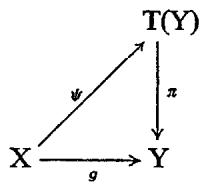
\includegraphics[keepaspectratio]{images/part001_bb2423ff.jpg}}

交换，其中 \(\pi\) 表示 T(Y) 到 Y 的典范投影。给定 \(\psi\) 等价于给定向量丛 \(g^{*}\mathrm{T}(\mathrm{Y})\) 的一个截面，即 T(Y) 在 g 下的逆像的一个截面。

提升的概念推广了向量场的概念（当 \(g = \operatorname{Id}_{\mathbf{X}}\) 时退化为向量场）；关于 \(\theta_{\xi}\) 和 \(i(\xi)\) 的定义与结果的重要部分也推广到提升；我们只简要指出其中几项。

8.6.2. 设 \(\psi: X \to T(Y)\) 是 \(g: X \to Y\) 的一个提升，并设 \(\omega\) 是一个 \(p\) 次、定义在 \(Y\) 上、取值于向量丛 \(F\)（其基底为 \(Y\)）的微分形式。当 \(p \geqslant 1\) 时，将微分形式 \(i(\psi,\omega)\)、或 \(i(\psi)\omega\)、或 \(i_{\psi}(\omega)\) 记在 X 上；它们的次数为 \(p-1\)，取值于 \(g^{*}\mathbf{F}\)，并满足

\[
i (\psi , \omega) _ {x} (v _ {1}, \dots , v _ {p - 1}) = \omega_ {g (x)} (\psi (x), T _ {x} (g). v _ {1}, \dots , T _ {x} (g). v _ {p - 1})\tag{1}
\]

对所有 \(x \in X\) 以及每个 \(v_1, \ldots, v_{p-1}\)（其元素属于 \(\mathbf{T}_x(X)\)），上述关系都成立。当 \(p = 0\) 时，令 \(i(\psi, \omega) = 0\)。称 \(i(\psi, \omega)\) 为 \(\psi\) 与 \(\omega\) 的内积；若 \(\psi\) 和 \(\omega\) 属于 \(\mathbf{C}^r\) 类，则 \(i(\psi, \omega)\) 也属于该类。设 \(\mathbf{F}' \times_{\mathbb{Y}} \mathbf{F}'' \to \mathbf{F}\) 是以 Y 为基底的向量丛的一个配对。对于 \(\omega' \in {}^\tau \Omega^{p'}(Y; F')\) 和 \(\omega'' \in {}^\tau \Omega^{p''}(Y; F'')\)，有

\[
i (\psi) \left(\omega^ {\prime} \wedge \omega^ {\prime \prime}\right) = (i (\psi) \omega^ {\prime}) \wedge g ^ {*} \omega^ {\prime \prime} + (- 1) ^ {p ^ {\prime}} g ^ {*} \omega^ {\prime} \wedge i (\psi) \omega^ {\prime \prime}.\tag{2}
\]

8.6.3. 例子

\begin{enumerate}
\def\labelenumi{\alph{enumi})}
\tightlist
\item
  X 上的向量场 \(\xi\) 定义了 g 在 T(Y) 中的提升 T(g) \(\circ\) \(\xi\)，并且有：
\end{enumerate}

\[
i (\mathrm{T} (g) \circ \xi) = i (\xi) \circ g ^ {*}.\tag{3}
\]

\begin{enumerate}
\def\labelenumi{\alph{enumi})}
\setcounter{enumi}{1}
\tightlist
\item
  Y 上的向量场 \(\eta\) 定义了 \(\eta \circ g\) 在 T(Y) 中的提升 \(g\)，并且有：
\end{enumerate}

\[
i (\eta \circ g) = g ^ {*} \circ i (\eta).\tag{4}
\]

\begin{enumerate}
\def\labelenumi{\alph{enumi})}
\setcounter{enumi}{2}
\tightlist
\item
  更一般地，设 \(h: \mathbf{Y} \to \mathbf{Z}\) 是 \(\mathbf{C}^{r+1}\) 类流形的态射。若 \(\psi\) 是 \(g\) 到 \(\mathbf{T}(\mathbf{Y})\) 的提升，则 \(\mathbf{T}(h) \circ \psi\) 是 \(h \circ g\) 到 \(\mathbf{T}(\mathbf{Z})\) 的提升，并且有：
\end{enumerate}

\[
i (\mathrm{T} (h) \circ \psi) = i (\psi) \circ h ^ {*}.\tag{5}
\]

若 \(\varphi\) 是 \(h\) 到 \(\mathrm{T}(Z)\) 的提升，则 \(\varphi \circ g\) 是 \(h \circ g\) 到 \(\mathrm{T}(Z)\) 的提升，并且有：

\[
i (\varphi \circ g) = g ^ {*} \circ i (\varphi).\tag{6}
\]

8.6.4（“无穷小变换”）。设 \(\psi\) 是 \(C^r\) 类的 \(g\) 的提升，且 \(\omega\) 是 Y 上取值于 Banach 空间 F、次数为 \(p\) 且属于 \(C^r\) 类的微分形式。X 上的微分形式

\[
d (i (\psi) \omega) + i (\psi) d \omega\tag{7}
\]

是次数为 \(p\) 的 \(\mathbf{C}^{r-1}\) 类形式；记为 \(\theta_{\psi}.\omega\)。

若 f 是 X 上的 \(C^{r}\) 类函数，则有

\[
\theta_ {f \psi}. \omega = d f \wedge i (\psi) \omega + f \theta_ {\psi}. \omega .\tag{8}
\]

8.6.5（“将 \(\theta_{\psi}.\omega\) 刻画为导数”）。保持 8.6.4 的假设。设 \(x\in X\)。则存在 \(x\) 的一个开邻域 U、K 中 0 的一个开邻域 I，以及一个 \(C^{r}\) 类态射 G: I × U → Y，具有下列两个性质：

\begin{enumerate}
\def\labelenumi{\alph{enumi})}
\item
  对每个 \(x \in \mathbf{U}\)，有 \(\mathbf{G}(0, x) = g(x)\)。
\item
  对每个 \(x \in \mathbf{U}\)，切向量 (1, 0) 在 \(\mathrm{T}_{(0,x)}(\mathrm{G})\) 下的像等于 \(\psi(x)\)。
\end{enumerate}

设 (U, I, G) 满足这些条件；对于每个 \(t \in \mathbf{I}\)，记从 U 到 Y 的映射 \(\mathbf{G}_t\) 为 \(x \mapsto \mathbf{G}(t, x)\)；置 \(\omega_t = \mathbf{G}_t^*(\omega)\)。对于每个 \(x \in \mathbf{X}\)，从 I 到 \(t \mapsto \omega_t(x)\) 的映射 \(\operatorname{Alt}^p(\mathrm{T}_x(\mathbf{X}), \mathbf{F})\) 属于 \(\mathbf{C}^r\) 类，且其在原点处的导数由下式给出

\[
\frac {d}{d t} (\omega_ {t} (x)) _ {t = 0} = (\theta_ {\psi}. \omega) (x).\tag{9}
\]

\subsection{结构的弱化}

本节假设 K = R。

8.7.1. 设 X 是 \(C^{s}\) 类流形，F 是 X 上的 \(C^{k}\) 类向量丛，其中 \(0 \leqslant k \leqslant s\)。若 \(0 \leqslant k' \leqslant k\)，则 F 上存在唯一的、以 X 为基底且属于 \(F_{k'}\) 类的向量丛结构 \(C^{k'}\)，使得 F 的每个向量坐标图都是 \(F_{k'}\) 的向量坐标图。称 \(F_{k'}\) 是通过弱化 F 的丛结构从 F 得到的。

8.7.2. 设 \(r \in \mathbf{N}_{\mathbb{R}}\) 且 \(r \leqslant s\)，令 \(\mathbf{X}_r\) 为以 \(\mathbf{C}^r\) 为底层的 \(\mathbf{X}\) 类流形（5.13.1）。切丛 \(\mathrm{T}(\mathbf{X}_r)\) 属于 \(\mathbf{C}^{r-1}\) 类；它是将属于 \(\mathrm{T}(\mathbf{X})\) 类的切丛 \(\mathbf{C}^{s-1}\) 的结构弱化而得到的丛。

设 F 是 X 上的 \(C^{k}\) 类向量丛，其中 \(0 \leqslant k \leqslant r - 1\)。X 上取值于 F 的 \(C^{k}\) 类微分形式与 \(X_{r}\) 上相应的微分形式典范地等同。本段其余部分所述的这些微分形式上的各种运算与此等同相容。

在本小册子的其余部分，我们常把这类其他结果的详细表述留给读者。

\subsection{几乎复流形与复流形}

本节假设 K = R，并记 X 为一个（实）\(\mathbf{C}^{r}\) 类流形，其中 \(r \in \mathbf{N}_{\mathbf{R}}\)。

8.8.1 (“复向量丛”). 以 X 为基底的 \(\mathbf{C}\) 上的向量丛（7.3.4）也称为以 X 为基底的复向量丛。若 M 是这样的向量丛，则称 M 的一个复向量坐标图为三元组 (U, \(\varphi\) , E)，其中 U 是 X 的开子集，E 是复 Banach 空间，且 \(\varphi\) 是从 \(M|_U\) 到平凡丛 \(E_U = U \times E\) 的复向量丛同构。其定义域 \((U_i,\varphi_i,E_i)\) 覆盖 X 的 M 的复向量坐标图族 \(U_i\) 称为 M 的复向量图册；每个复向量丛都具有一个复向量图册（7.3.3）。

有时用 C-向量代替复向量。同样，在谈论 R 上的向量丛、该丛的普通向量坐标图等对象时，有时用“实向量”或“R-向量”代替“向量”。

设 M 是以 X 为基底的复向量丛。M 的（实）底层向量丛（7.3.3）存在且仅存在一个自同构 j，其在每个纤维上的限制是乘以 C 的元素 i；j 的平方等于 -1。反之，若 M 是以 X 为基底的（实）向量丛，且 j 是 M 的满足 \(j^{2} = -1\) 的自同构，则 M 上存在唯一的复向量丛结构，以 M 为其（实）底层向量丛，并且其中 j 是乘以 i 的映射。

8.8.2（“向量丛的复化”）。对每个（实）Banach 空间 \(\tau\)，令 \(\tau(E) = E \otimes C\)，并对（实）Banach 空间的每个态射 \(E\)，令 \(\tau(u) = u \otimes Id_{C}\)，由此定义一个向量函子 \(u: E \to E'\)。

若 F 是以 X 为基底的 \(C^{k}\) 类向量丛（\(0 \leqslant k \leqslant r\)），则其在向量函子 \(\tau\) 下的像记为 \(F \otimes C\)。在 \(F \otimes C\) 上存在唯一的、以 X 为基底且属于 \(C^{k}\) 类的复向量丛结构；它与其（实）向量丛结构相容，并在每个纤维 \((\mathbf{F} \otimes \mathbf{C})_{x} = \mathbf{F}_{x} \otimes \mathbf{C}\) 上赋予其典范的复 Banach 空间结构（EVT, II, § 8, n° 1, Example）。赋予此结构后，称 \(F \otimes C\) 为 F 的复化。

设 U 是 X 的开子集；典范映射

\[
\mathcal {S} _ {\mathrm{F}} ^ {k} (\mathrm{U}) \otimes \mathbf {C} \rightarrow \mathcal {S} _ {\mathrm{F} \otimes \mathbf {C}} ^ {k} (\mathrm{U})
\]

是一个同构，借此将这两个空间等同。若 \(s \in \mathcal{S}_{\mathrm{F} \otimes \mathrm{C}}^{k}(\mathrm{U})\)，\(\sigma, \tau\) 是 \(\mathcal{S}_{\mathrm{F}}^{k}(\mathrm{U})\) 的元素且满足 \(s = \sigma + i\tau\)，则称它们为 \(s\) 的实部和虚部；截面 \(\bar{s} = \sigma - i\tau\) 称为 \(s\) 的共轭。

特别地，丛 \(\mathrm{T}(\mathrm{X}) \otimes \mathbf{C}\) 的截面称为 X 上的复向量场。

以 X 为底的复向量丛 H 的典范同构 \(\operatorname{Alt}_{\mathbf{R}}^{p}(\mathrm{T}_{x}(\mathrm{X});\mathrm{H})\to\operatorname{Alt}_{\mathbf{C}}^{p}(\mathrm{T}_{x}(\mathrm{X})\otimes\mathbf{C};\mathbf{H})\) 定义了从 \(\operatorname{Alt}_{\mathbf{R}}^{p}(\mathrm{T}(\mathrm{X});\mathrm{H})\) 到 \(\operatorname{Alt}_{\mathbf{C}}^{p}(\mathrm{T}(\mathrm{X})\otimes\mathbf{C};\mathbf{H})\) 的复向量丛典范同构，称为典范同构（7.8.5）；借此将这两个丛等同。设 \(\omega\) 是该丛的一个截面，换言之，是 X 上取值于 H 的 p 次微分形式；设 \(\zeta\) 是复向量场，其实部为 \(\xi\)，虚部为 \(\eta\)。置：

\[
i (\zeta , \omega) = i (\xi , \omega) + i. i (\eta , \omega).
\]

若 H 是平凡丛，置

\[
\theta_ {\zeta}. \omega = \theta_ {\xi}. \omega + i \theta_ {\eta}. \omega .
\]

同样，按线性将括号延拓到复向量场。前面各号的公式仍然成立。

8.8.3. X 上的一个 \(C^{k}\) 类几乎复结构（\(k \leqslant r - 1\)）是指在 \(\mathrm{T}(\mathrm{X})\) 上给定一个 \(C^{k}\) 类复向量丛结构，其底层实结构是 \(\mathrm{T}(\mathrm{X})\) 的自然结构。这种结构等价于给定 \(j\) 的一个 \(C^{k}\) 类自同构 \(\mathrm{T}(\mathrm{X})\)，满足 \(j^{2} = -1\)。

取这样一个结构。将 \(j\) 延拓为 \(\mathbf{C}\) 的一个 \(\mathrm{T}(\mathrm{X}) \otimes \mathbf{C}\)-自同构。存在 \(\mathrm{T}(\mathrm{X}) \otimes \mathbf{C}\) 作为两个复子丛直和的唯一分解：

\[
\mathbf {T} (\mathrm{X}) \otimes \mathbf {C} = \mathbf {T} ^ {\prime} (\mathrm{X}) \oplus \mathbf {T} ^ {\prime \prime} (\mathrm{X})\tag{1}
\]

使得 \(j\) 在 \(i\) 上与乘以 \(\mathbf{T}'(\mathbf{X})\) 一致，在 \(-i\) 上与乘以 \(\mathbf{T}''(\mathbf{X})\) 一致。\(p'\) 到 \(\mathbf{T}(\mathbf{X}) \otimes \mathbf{C}\) 的投影算子 \(\mathbf{T}'(\mathbf{X})\) 等于 \(\frac{1}{2}(1 - ij)\)；\(p'' = 1 - p'\) 到 \(\mathbf{T}(\mathbf{X}) \otimes \mathbf{C}\) 的投影算子 \(\mathbf{T}''(\mathbf{X})\) 等于 \(\frac{1}{2}(1 + ij)\)。复合映射

\[
\pi^ {\prime} \colon \mathrm{T} (\mathrm{X}) \rightarrow \mathrm{T} (\mathrm{X}) \otimes \mathbf {C} \xrightarrow {p ^ {\prime}} \mathrm{T} ^ {\prime} (\mathrm{X})
\]

\[
\pi^ {\prime \prime}: \mathrm{T} (\mathrm{X}) \rightarrow \mathrm{T} (\mathrm{X}) \otimes \mathbf {C} \xrightarrow {p ^ {\prime \prime}} \mathrm{T} ^ {\prime \prime} (\mathrm{X})
\]

是 R-同构；第一个将 j 映为乘以 i，第二个将 j 映为乘以 -i。

8.8.4（“\((p,q)\) 型的形式”）。保持前一号的假设和记号。设 F 是以 X 为基底的复向量丛，p 和 q 是两个 \(\geqslant0\) 的整数，且 \(n=p+q\)。设 \(\omega\) 是 X 的开集 U 上取值于 F 的 n 次微分形式；按照（8.8.2）将 \(\omega\) 与 \(\operatorname{Alt}_{\mathbf{C}}^{n}(\operatorname{T}(\mathbf{X})\otimes\mathbf{C};\mathbf{F})\) 的一个截面等同。若对所有 \(\omega\) 都有下式，则称 \((p,q)\) 为 \(x\in U\) 型：

\[
\omega_ {x} (v _ {1}, \dots , v _ {n}) = 0
\]

只要有 \(p + 1\) 个向量 \(v_i\) 属于 \(T_x'(X)\)，或有 \(q + 1\) 个向量 \(v_i\) 属于 \(T_x''(X)\)，该式就成立。若将 \(\bigwedge^n T_x(X) \otimes C\) 与各空间 \(\bigwedge^{m'} T_x'(X) \otimes \bigwedge^{m''} T_x''(X)\)（其中 \(m' + m'' = n\)）的直和等同（A, III, p. 85），并将 \(\omega_x\) 与一个 \(C\)-线性形式等同，该形式定义在 \(\bigwedge^n T_x(X)\) 上，则这等价于说，\(\omega_x\) 在 \(\bigwedge^{m'} T_x'(X) \otimes \bigwedge^{m''} T_x''(X)\) 上对 \((m', m'') \neq (p, q)\) 为零。

对于每一对满足 \((p,q)\) 的 \(\geqslant0\) 整数 \(p+q=n\)，存在且仅存在一个 \(\operatorname{Alt}^{p,q}(\mathrm{T}(\mathrm{X});\mathrm{F})\) 的复向量子丛 \(\operatorname{Alt}^{n}(\mathrm{T}(\mathrm{X});\mathrm{F})\)，使得其在 X 的开集 U 上的截面正是 X 上取值于 F 的 \((p,q)\) 型微分形式。向量丛 \(\operatorname{Alt}^{n}(\mathrm{T}(\mathrm{X});\mathrm{F})\) 是对于 \(\operatorname{Alt}^{p,q}(\mathrm{T}(\mathrm{X});\mathrm{F})\)、\(p\geqslant0\) 且 \(q\geqslant0\) 的向量丛 \(p+q=n\) 的直和。每个取值于 F 的 n 次微分形式 \(\omega\) 都唯一分解为

\[
\omega = \sum_ {p + q = n} \omega_ {p, q}
\]

其中 \(\omega_{p,q}\) 是一个 \((p,q)\) 型形式，称为 \((p,q)\) 的 \(\omega\) 型分量。若 \(\omega\) 属于 \(\mathbf{C}^h\) 类，其中 \(0 \leqslant h \leqslant k\)，则其各分量也具有同样性质。

例子

\begin{enumerate}
\def\labelenumi{\alph{enumi})}
\item
  n 次微分形式是 \((n, 0)\) 型，当且仅当它是 \(\mathbf{C}\)-多线性的。
\item
  设 \(\mathbf{F}'\)、\(\mathbf{F}''\) 和 \(\mathbf{F}\) 是三个复向量丛，且 \(\mathbf{F}' \times_{\mathbf{X}} \mathbf{F}'' \to \mathbf{F}\) 是一个 \(\mathbf{C}\)-双线性配对。若 \(\omega'\)（分别为 \(\omega''\)）是取值于 \((p',q')\)（分别为 \((p'',q'')\)）的 \(\mathbf{F}'\) 型（分别为 \(\mathbf{F}''\) 型）微分形式，则微分形式 \(\omega' \wedge \omega''\) 是 \((p' + p'',q' + q'')\) 型。
\item
  假设 F 是一个（实）向量丛的复化（8.8.2）。若 \(\omega\) 是取值于 F 的 \((p, q)\) 型微分形式，则其共轭 \(\overline{\omega}\)（8.8.2）是 \((q, p)\) 型。
\end{enumerate}

8.8.5. 除前述假设外，再假设 \(k \geqslant 1\)。以下三个条件等价：

\begin{enumerate}
\def\labelenumi{(\roman{enumi})}
\item
  对 X 的每个开集 U，以及 U 上每一对 \((\xi, \eta)\) 类复向量场 \(C^{k}\)，若对所有 \(\xi(x)\) 都有 \(\eta(x)\) 和 \(\mathrm{T}_{x}^{\prime}(\mathrm{X})\) 属于 \(x \in U\)，则对所有 \([\xi, \eta](x) \in \mathrm{T}_{x}^{\prime}(\mathrm{X})\) 都有 \(x \in U\)。
\item
  对 X 的每个开集 U，以及 U 上每一对 \((\xi, \eta)\) 类（实）向量场 \(C^{k}\)，有
\end{enumerate}

\[
[ \xi , \eta ] + j [ j \xi , \eta ] + j [ \xi , j \eta ] - [ j \xi , j \eta ] = 0.
\]

\begin{enumerate}
\def\labelenumi{(\roman{enumi})}
\setcounter{enumi}{2}
\tightlist
\item
  对 X 的每个开集 U，以及 U 上每个属于 \(\omega\) 类的 \((1,0)\) 型复微分形式 \(C^{k}\)，\((0,2)\) 的 \(d\omega\) 型分量为零。
\end{enumerate}

假设这些条件成立。设 \(\omega\) 是 X 的开集 U 上取值于复 Banach 空间 F、属于 \((p,q)\) 类且满足 \(\mathbf{C}^h\) 的 \(1\leqslant h\leqslant k\) 型微分形式。将 \(d'\omega\) 的 \(d''\omega\) 型（分别为 \((p+1,q)\) 型）分量记为 \((p,q+1))\)（分别为 \(d\omega\)）；此时 \(d\omega\) 的其他分量均为零，并且有

\[
d \omega = d ^ {\prime} \omega + d ^ {\prime \prime} \omega .\tag{2}
\]

若 \(k\geqslant 2\)，则有

\[
d ^ {\prime} (d ^ {\prime} \omega) = 0, d ^ {\prime \prime} (d ^ {\prime \prime} \omega) = 0, d ^ {\prime} (d ^ {\prime \prime} \omega) + d ^ {\prime \prime} (d ^ {\prime} \omega) = 0.\tag{3}
\]

采用 8.8.4 的记号，例 \(b\)，有

\begin{enumerate}
\def\labelenumi{(\arabic{enumi})}
\setcounter{enumi}{3}
\tightlist
\item
\end{enumerate}

\[
d ^ {\prime} \left(\omega^ {\prime} \wedge \omega^ {\prime \prime}\right) = d ^ {\prime} \left(\omega^ {\prime}\right) \wedge \omega^ {\prime \prime} + (- 1) ^ {p ^ {\prime} + q ^ {\prime}} \omega^ {\prime} \wedge d ^ {\prime} \left(\omega^ {\prime \prime}\right)\tag{4}
\]

\[
d ^ {\prime \prime} (\omega^ {\prime} \wedge \omega^ {\prime \prime}) = d ^ {\prime \prime} (\omega^ {\prime}) \wedge \omega^ {\prime \prime} + (- 1) ^ {p ^ {\prime} + q ^ {\prime}} \omega^ {\prime} \wedge d ^ {\prime \prime} (\omega^ {\prime \prime})\tag{5}
\]

结合 8.8.4 的例 c)，有

\[
d ^ {\prime} (\overline {{\omega}}) = \overline {{d ^ {\prime \prime} (\omega)}}.\tag{6}
\]

在公式 (4) 和 (5)（分别为 (6)）中，微分形式 \(\omega'\) 和 \(\omega''\)（分别为 \(\omega\)）均假定属于 \(\mathbf{C}^1\) 类。

8.8.6（“复流形的几乎复结构”）。设 \(X^c\) 是一个复解析流形，其底层实解析流形为 X（5.14.2.a)）。将丛 \(\mathrm{T}(\mathrm{X})\) 与复向量丛 \(\mathrm{T}(X^c)\) 的（实）底层向量丛等同，由此在 X 上赋予一个 \(C^\omega\) 类几乎复结构，称为由 X 上给定的复解析流形结构定义的几乎复结构。该几乎复结构满足 8.8.5 的条件 (i) 至 (iii)；特别地，8.8.5 的算子 \(d'\) 和 \(d''\) 有定义。若 \(f: X^c \to Y^c\) 是复解析流形的态射，则 \(f^*\) 与算子 \(d'\) 和 \(d''\) 可交换。

8.8.7. 保持 8.8.6 的假设和记号。令 \(\overline{\mathbf{X}}^c\) 为 \(\mathbf{X}^c\) 的共轭（5.14.2.b)）。通过对角映射 \(x \mapsto (x, x)\) 将 X 嵌入复流形 \(\mathbf{X}^c \times \overline{\mathbf{X}}^c\) 中，并令 \(g\) 为 \((x, y) \mapsto (y, x)\) 的反自同构 \(\mathbf{X}^c \times \overline{\mathbf{X}}^c\)。对 \((\mathbf{X}^c \times \overline{\mathbf{X}}^c, g)\) 是 X 的一个复化（5.14.8）。特别地，对每个 \(x \in \mathbf{X}\)，切空间 \(\mathrm{T}_x(\mathrm{X}^c \times \overline{\mathrm{X}}^c)\) 与 \(\mathrm{T}_x(\mathrm{X}) \otimes \mathbf{C}\) 等同；在此等同下，\(\mathrm{T}_x(\mathrm{X}^c \times \{x\})\) 对应于 \(\mathrm{T}_x'(\mathrm{X})\)，而 \(\mathrm{T}_x(\{x\} \times \overline{\mathrm{X}}^c)\) 对应于 \(\mathrm{T}_x''(\mathrm{X})\)。

8.8.8. 假设 \(r = \omega\)；X 上满足 8.8.5 的等价条件 (i) 至 (iii) 的任一 \(C^\omega\) 类几乎复结构，都是由 \(X\) 上唯一一个复解析流形结构定义的几乎复结构。\(^{(1)}\)

8.8.9（“全纯形式”）。恢复 8.8.6 的假设和记号，并设 F 是复 Banach 空间。\(\mathbf{X}^c\) 上取值于 F 的解析微分形式（换言之，复解析微分形式）仍称为全纯微分形式；将 \(\mathrm{T}(\mathbf{X}^c)\) 与 \(\mathrm{T}(\mathbf{X})\) 等同，就把它们与 X 上的（实解析）微分形式等同。对于 X 上取值于 F、属于 \(\omega\) 类且次数为 \(p\) 的微分形式 \(\mathbf{C}^k\)，其中 \(k \geqslant 1\)，它是全纯的充要条件是它属于 \((p, 0)\) 型且满足 \(d''\omega = 0\)。

设 \(\xi\) 是 X 上的向量场。若 \(\xi\) 是从 \(X^c\) 到 \(T(X^c) = T(X)\) 的复解析映射，换言之，是 \(X^c\) 上的复解析向量场，则称其为全纯的。在此情形，若 \(\omega\) 是 X 上取值于 F 的全纯微分形式，则形式 \(\theta_{\xi}.\omega\)（分别为 \(i(\xi)\omega\)）无论将 \(\xi\) 看作 \(X^c\) 上的复解析向量场、将 \(\omega\) 看作 \(\Omega^p(X^c; F)\) 的元素，还是将 \(\xi\) 看作 X 上的向量场、将 \(\omega\) 看作 \(\Omega^p(X; F)\) 的元素，都相同。此外，令 \(\xi' = \pi'(\xi)\) 和 \(\xi'' = \pi''(\xi)\) 分别为 \(\xi\) 在 \(T'(X)\) 和 \(T''(X)\) 中的分量（8.8.3）；有

\begin{enumerate}
\def\labelenumi{(\arabic{enumi})}
\setcounter{enumi}{6}
\tightlist
\item
\end{enumerate}
\[
\theta_ {\xi}. \omega = \theta_ {\xi^ {\prime}}. \omega , \quad \theta_ {\xi^ {\prime \prime}}. \omega = 0,\tag{7}
\]

\[
i (\xi) \omega = i (\xi^ {\prime}) \omega , i (\xi^ {\prime \prime}) \omega = 0.\tag{8}
\]

8.8.10. 例。--- 假设 \(X^{c}\) 是 \(C^{n}\) 的开子集，并记 \(z^{1},\ldots,z^{n}\) 为 \(X^{c}\) 上的坐标函数。对于 \(1\leqslant k\leqslant n\)，置 \(z^{k}=x^{k}+iy^{k}\)，其中 \(x^{k}\) 和 \(y^{k}\) 取实值。考虑由坐标系 \((\partial/\partial z^{k})\) 定义的 \(\mathrm{T}(\mathrm{X}^{c})\) 的切标架 \((z^{k})\)，以及由坐标系 \((\partial/\partial x^{k},\partial/\partial y^{k})\) 定义的 \(\mathrm{T}(\mathrm{X})\) 的切标架 \((x^{k},y^{k})\)（8.1.5）。有 \(j(\partial/\partial x^{k})=\partial/\partial y^{k}\)，且 \(\partial/\partial z^{k}\) 在映射 \(\pi^{\prime}\colon\mathrm{T}(\mathrm{X})=\mathrm{T}(\mathrm{X}^{c})\to\mathrm{T}^{\prime}(\mathrm{X})\)（8.8.3）下的像等于

\[
\frac {1}{2} (\partial / \partial x ^ {k} - i \partial / \partial y ^ {k});
\]

通常仍将其记为 \(\partial/\partial z^{k}\)。\(^{(2)}\) 该向量场 \(\partial/\partial z^{k}\) 的复共轭向量场记为 \(\partial/\partial\bar{z}^{k}\)；有

\[
\partial / \partial \bar {z} ^ {k} = \frac {1}{2} (\partial / \partial x ^ {k} + i \partial / \partial y ^ {k}).\tag{9}
\]

若 f 是 X 上取值于复 Banach 空间 F 的 \(C^{1}\) 类函数，则微分形式 \(d'f\) 和 \(d''f(8.8.5)\) 由下式给出

\[
d ^ {\prime} f = \sum_ {1 \leqslant k \leqslant n} \frac {\partial f}{\partial z ^ {k}} d z ^ {k}, d ^ {\prime \prime} f = \sum_ {1 \leqslant k \leqslant n} \frac {\partial f}{\partial \bar {z} ^ {k}} d \bar {z} ^ {k}.\tag{10}
\]

\(^{(1)}\) 若 X 是有限维的，则对于属于 \(C^k\) 类且满足 \(k = \dim X\) 的几乎复结构，上述结论仍然成立（参见 A. Newlander 和 L. Nirenberg, "Complex analytic coordinates in almost complex manifolds," Ann. of Math. LXX (1957), pp. 391--404）。

\(^{(2)}\) 须注意：将 \(\mathrm{T}(X^c)\) 与 \(\mathrm{T}(X)\) 典范等同，并不会把 \(\partial/\partial z^k\) 上的向量场 \(X^c\) 变为 X 上的向量场 \(\partial/\partial z^k\)，而是变为向量场 \(\partial/\partial z^k+\partial/\partial\bar z^k\)。然而，记作 \(\partial/\partial z^k\) 的两个向量场在全纯微分形式（8.8.9）上的取值相同；事实上，只有对这些形式才能应用 \(X^c\) 的向量场。

回顾有

\[
d f = d ^ {\prime} f + d ^ {\prime \prime} f
\]

\[
d z ^ {k} = d x ^ {k} + i d y ^ {k} \quad d \bar {z} ^ {k} = d x ^ {k} - i d y ^ {k}.
\]

若 \(\mathbf{A}=(i_{1},\ldots,i_{p})\) 是属于区间 \([1,n]\) 的严格递增整数序列，置

\[
d z ^ {A} = d z ^ {i _ {1}} \wedge \dots \wedge d z ^ {i _ {p}}
\]

并将 \(d\bar{z}^{\mathrm{A}}\) 的共轭记为 \(dz^{\mathrm{A}}\)。每个取值于 F 的 \(\omega\) 型微分形式 \((p,q)\) 都唯一地写成

\[
\omega = \sum_ {\mathrm{A}, \mathrm{B}} f _ {\mathrm{A}, \mathrm{B}} d z ^ {\mathrm{A}} \wedge d \bar {z} ^ {\mathrm{B}}\tag{11}
\]

其中 A（分别为 B）遍历由 \(p\) 中的 \(q\)（分别为 \([1, n]\)）个元素组成的严格递增序列集，\(f_{A,B}\) 是取值于 F 的函数。若 \(\omega\) 属于 \(\mathbf{C}^k\) 类，其中 \(k \geqslant 1\)，则函数 \(f_{A,B}\) 也具有同样的类，并且有

\begin{enumerate}
\def\labelenumi{(\arabic{enumi})}
\setcounter{enumi}{11}
\tightlist
\item
\end{enumerate}
\[
d ^ {\prime} \omega = \sum_ {A, B} d ^ {\prime} f _ {A, B} \wedge d z ^ {A} \wedge d \bar {z} ^ {B}\tag{12}
\]

\[
d ^ {\prime \prime} \omega = \sum_ {\mathbf {A}, \mathbf {B}} d ^ {\prime \prime} f _ {\mathbf {A}, \mathbf {B}} \wedge d z ^ {\mathbf {A}} \wedge d \bar {z} ^ {\mathbf {B}}.\tag{13}
\]

\section{微分方程与叶状结构}

在第 9.1、9.2 和 9.3 号中，假设 K 的特征为 0；在第 9.4 号中，假设 K 的特征为 \(p \neq 0\)。

\subsection{积分曲线}

本节中，X 表示一个 \(C^{r}\) 类流形，\(\xi\) 是 X 上的 \(C^{s}\) 类向量场，其中 r、s 属于 \(N_{K}\)，且 \(s \leqslant r - 1\)。

9.1.1. 设 I 是 K 的开子集，且 \(f: \mathbf{I} \to \mathbf{X}\) 是从 I 到 X 的 \(\mathbf{C}^k\) 类映射（\(k \in \mathbf{N}_{\mathbb{K}}\)，\(k \leqslant r\)）。对于 \(t \in \mathbf{I}\)，将向量 \(f'(t)\) 记为 \(\mathrm{T}_t(f)(1) \in \mathrm{T}_{f(t)}(\mathbf{X})\)；该向量有时称为 \(f\) 在时刻 \(t\) 的速度。当 X 是 Banach 空间时，\(f'(t)\) 是 \(f\) 在 \(t\) 处的导数。

若有下式，则称 \(f\) 是 \(\xi\) 的积分曲线：

\[
f ^ {\prime} (t) = \xi (f (t))\tag{1}
\]

对所有 \(t \in I\) 都成立。这样的曲线属于 \(C^{s+1}\) 类。

若 \(x\) 是 X 的一点，则将满足 \(\xi\) 且 \(x\) 的 \(f: I \to X\) 的积分曲线 \(\xi\) 称为以 \(0 \in I\) 为起点的 \(f(0) = x\) 的积分曲线；对每个 \(x \in X\)，都存在一条以 \(\xi\) 为起点的 \(x\) 的积分曲线，它定义在 K 中 0 的某个适当开邻域上。

若 \(f: \mathbf{I} \to \mathbf{X}\) 是 \(\xi\) 的积分曲线且 \(a \in \mathbf{K}\)，则从 \(t \mapsto f(t - a)\) 到 \(\mathbf{I} + a\) 的映射 \(\mathbf{X}\) 是 \(\xi\) 的积分曲线。

设 \(f_{1}\colon\mathbf{I}_{1}\to\mathbf{X}\) 和 \(f_{2}\colon\mathbf{I}_{2}\to\mathbf{X}\) 是 \(\xi\) 的两条积分曲线，且 \(t\in\mathbf{I}_{1}\cap\mathbf{I}_{2}\)。若 \(f_{1}(t)=f_{2}(t)\)，则映射 \(f_{1}\) 和 \(f_{2}\) 在 \(t\) 的某个邻域内一致。

9.1.2（“流”）。设 W 是 X × K 的开子集。对每个 x ∈ X，记 W \(_{x}\) 为满足 (x, t) ∈ W 的 t ∈ K 所成的集合。称定义域为 W 的 ξ 的一个积分流为从 W 到 X 的 C \(^{k}\) 类映射 f（k ≤ r），满足：对每个 x ∈ X，由 f \(_{x}\) (t) = f(x, t) 定义的映射 f \(_{x}\) : W \(_{x}\) → X 是 ξ 的积分曲线，并且只要 (x, 0) ∈ W，就有 f(x, 0) = x。

对每个点 \(x \in X\)，存在一个 \(\xi\) 的 \(\mathbf{C}^s\) 类积分流，其定义域是 \((x, 0)\) 中 \(X \times K\) 的某个邻域。定义在 \(\xi\) 的某个邻域内的两个 \((x, 0)\) 的积分流在 \((x, 0)\) 的某个邻域内一致。

设 \(x\in X\)，且 \(f\) 是 \(\xi\) 的一个积分流，其定义域 W 是 \((x,0)\) 的一个邻域。存在 \((x,0,0)\) 在 \(X \times K \times K\) 中的一个邻域 V，使得若 \((x,t_{1},t_{2})\in\mathrm{V}\)，则有

\[
(x, t _ {1}) \in \mathbf {W}, \quad (f (x, t _ {1}), t _ {2}) \in \mathbf {W}, \quad (x, t _ {1} + t _ {2}) \in \mathbf {W}
\]

并且

\[
f (f (x, t _ {1}), t _ {2}) = f (x, t _ {1} + t _ {2}).\tag{2}
\]

若 X 是仿紧的，或者 X 是分离的且 K = R 或 C，则存在一个 \(\xi\) 的积分流，其定义域是 \(X \times \{0\}\) 的一个邻域。

9.1.3（“实情形”）。假设 K = R 且 X 是分离的。将定义域为 R 的开区间的 \(\xi\) 的任意积分曲线称为 \(\xi\) 的积分弧。若 \(f_{1}\) 的两条积分弧 \(f_{2}\) 和 \(\xi\) 分别定义在区间 \(I_{1}\) 和 \(I_{2}\) 上，并在 \(I_{1} \cap I_{2}\) 的一点处相同，则它们在 \(I_{1} \cap I_{2}\) 上一致。

对每个点 \(x \in X\)，存在一条以 \(x\) 为起点的积分弧，并且唯一存在 \(f_x: I_x \to X\)，使得对于每条积分弧 \(f: I \to X\)（以 \(x\) 为起点），都有 \(I \subset I_x\) 且 \(f = f_x|I\)。弧 \(f_x\) 称为向量场 \(\xi\) 以 \(x\) 为起点的最大积分弧，其定义域 \(I_x\) 有时称为点 \(x\) 对向量场 \(\xi\) 的寿命区间。

若 \(I_x = ]-a_-,a_+[\)（且若 \(a_+\) 有限，则 \(f_x\) 在区间 \([0,a_+[\) 上的限制是从 \([0,a_+[\) 到 X 的真映射），则特别地，\(f_x(t)\) 当 \(t\) 趋于 \(a_+\) 时没有极限。

9.1.4. 采用 9.1.3 的记号和假设，令 \(\Omega\) 为满足 \((x,t)\in\mathbf{X}\times\mathbf{R}\) 的对 \(t\in\mathbf{I}_{x}\) 所成的集合。它是 \(\mathbf{X}\times\mathbf{R}\) 中的开集，且由 \(f\colon\Omega\to\mathbf{X}\) 定义的映射 \(f(x,t)=f_{x}(t)\) 是定义域为 \(\xi\) 的 \(\Omega\) 的积分流。

由 \(\alpha_{+}\) 定义的函数 \(\alpha_{-}: X \to ]0,+\infty]\) 和 \(I_{x} = ]-\alpha_{-}(x),\alpha_{+}(x)[\) 是下半连续的。对于 \((x, t) \in \Omega\) 且 \(y = f(x, t)\)，有 \(\alpha_{+}(y) = \alpha_{+}(x) - t\) 和 \(\alpha_{-}(y) = \alpha_{-}(x) + t\)。

若 \(t_1 \in \mathbf{I}_x\) 且 \(t_2 \in \mathbf{I}_{f(x, t_1)}\)，则 \(t_1 + t_2 \in \mathbf{I}_x\)，并且

\[
f (f (x, t _ {1}), t _ {2}) = f (x, t _ {1} + t _ {2}).\tag{3}
\]

若函数 \(\alpha_{+}\)（分别为 \(\alpha_{-}\)）在 X 上有一个 \(>0\) 的常数作为下界，则它是常数且等于 \(+\infty\)。

在下列每种情形中，都有 \(\alpha_{+} = \alpha_{-} = +\infty\)（换言之，有 \(\Omega = \mathbf{X} \times \mathbf{R}\)）：

\begin{enumerate}
\def\labelenumi{(\roman{enumi})}
\item
  向量场 \(\xi\) 具有紧支集（例如 X 是紧的）；
\item
  存在一个保持 \(\xi\) 的 X 的传递自同构群；
\item
  X 上存在一个黎曼结构，使得 X 是完备的且 \(\xi\) 有界。
\end{enumerate}

若 \(\Omega = X \times R\)，则映射 \(f: X \times R \to X\) 是 \(C^s\) 类的群流形 \(R\) 在流形 \(X\) 上的右作用律，cf.~5.12.5。

9.1.5（“复情形”）。假设 K = C 且 X 是分离的。对于每个 \(a \in ]0, +\infty]\)，记 \(D_a\) 为 C 中以 0 为中心、半径为 a 的开圆盘。对于每个 \(x \in X\)，存在唯一的数 \(\rho(x) \in ]0, +\infty]\) 以及唯一的积分曲线 \(f_x: D_{\rho(x)} \to X\)，其起点为 \(x\)，使得对于每个 \(a \in ]0, +\infty]\) 以及每条积分曲线 \(f: \mathrm{D}_a \to \mathrm{X}\)，其起点为 \(x\)，都有 \(a \leqslant \rho(x)\) 且 \(f = f_x | \mathrm{D}_a\)。

对于每个 \(\lambda\in\mathbf{C}\)，令 \(\alpha_{\lambda}(x)\) 为点 \(x\) 对于实流形上的向量场 \(\lambda\xi\) 的寿命区间的上界。则有 \(\rho(x)=\inf_{|\lambda|=1}\alpha_{\lambda}(x)\)。

满足 \(\Delta\) 的对 \((x,t)\in X\times\mathbf{C}\) 所成的集合 \(t\in D_{\rho(x)}\) 是 \(X\times\mathbf{C}\) 中的开集，且由 \(f:\Delta\to X\) 定义的映射 \(f(x,t)=f_x(t)\) 是 \(\xi\) 的积分流。函数 \(\rho:X\to ]0,+\infty]\) 是下半连续的。对于 \((x,t)\in\Delta\) 且 \(y=f(x,t)\)，有 \(\rho(y)\geqslant\rho(x)-|t|\)。若 \(\rho\) 在 \(X\) 上有一个 \(>0\) 的常数作为下界，则 \(\rho = +\infty\) 且 \(\Delta = X \times C\)。

当 \(\Delta = X \times C\) 时，映射 \(f: X \times C \to X\) 是群流形 \(C\) 在流形 \(X\) 上的右作用律。

9.1.6. 设 \(\varphi: X \to Y\) 是流形的态射，\(\eta\) 是 Y 上的向量场，且 \(\xi\) 通过 \(\varphi\) 与 \(\eta\) 相关（参见 8.2.6）。若 \(f: I \to X\) 是 \(\xi\) 的积分曲线，则映射 \(\varphi \circ f: I \to Y\) 是 \(\eta\) 的积分曲线。若 \(K = R\) 且 X 和 Y 是分离的，则对于每个 \(x \in X\)，点 \(x\) 对向量场 \(\xi\) 的寿命区间包含于点 \(\varphi(x)\) 对向量场 \(\eta\) 的寿命区间。若此外 \(\varphi\) 是真映射，则这两个区间相等。

9.1.7（“含时方程”）。设 W 是 X × K 的开子集，且 Ξ: W → T(X) 是 pr \(^{s}\) : W → X 的 C \(_{1}\) 类提升，即从 W 到 T(X) 的 C \(^{s}\) 类映射，并满足对所有 (x, t) ∈ W，Ξ(x, t) 属于 T \(_{x}\) (X)。将从 K 的开子集 I 到 X 的 C \(^{k}\) 类映射 f 称为 Ξ 的积分曲线，其中 k ∈ N \(_{K}\) 且 k ≤ r，并且对所有 t ∈ I 都有

\[
(f (t), t) \in \mathrm{W},\qquad f ^ {\prime} (t) = \Xi (f (t), t).
\]

设 \(\eta\) 为 W 上的 \(C^s\) 类向量场，它由 \(\eta(x, t) = (\Xi(x, t), (t, 1))\) 定义。对于从 K 的开子集 I 到 X 的映射 \(f\)，要使其成为 \(\Xi\) 的积分曲线，充要条件是 \(t \mapsto (f(t), t)\) 按 9.1.1 的意义是 \(\eta\) 的积分曲线。

设 \(g: \mathbf{I} \to \mathbf{W}\) 是 \(\eta\) 的积分曲线，且 \(t_0\) 是 \(\mathbf{I}\) 中满足 \(\operatorname{pr}_2(g(t_0)) = t_0\) 的一点。满足 \(t \in \mathbf{I}\) 的 \(\operatorname{pr}_2(g(t)) = t\) 所成的集合是 \(t_0\) 的一个邻域；若 \(\mathbf{I}\) 连通，则该集合与 \(\mathbf{I}\) 重合。

9.1.8（“参数与初始条件”）。设 Z 是 \(C^{r}\) 类流形，W 是 X × K × Z 的开子集，且 \(\Xi\) 是 \(C^{s}\) 的 \(pr_{1}: W \to X\) 类提升。若 \(z \in Z\)，记满足 \(W_{z}\) 的 \((x, t) \in X \times K\) 所成的集合为 \((x, t, z) \in W\)，并将从 \(\Xi_{z}\) 到 T(X) 的映射 \((x, t) \mapsto \Xi(x, t, z)\) 记为 \(W_{z}\)。

设 \((x_0, t_0, z_0)\) 是 W 的一点。则 W 中存在 \(X_1 \times I_1 \times Z_1\) 的一个开邻域 \((x_0, t_0, z_0)\) 以及一个 \(C^s\) 类映射

\[
f \colon X _ {1} \times I _ {1} \times I _ {1} \times Z _ {1} \rightarrow X
\]

使得对于任意 \((x_{1}, t_{1}, z_{1}) \in \mathbf{X}_{1} \times \mathbf{I}_{1} \times \mathbf{Z}_{1}\)，映射 \(t \mapsto f(x_{1}, t_{1}, t, z_{1})\) 是 \(\Xi_{z_{1}}\) 的积分曲线（按 9.1.7 的意义），并满足关系 \(f(x_{1}, t_{1}, t_{1}, z_{1}) = x_{1}\)。

两个映射

\[
f _ {1}: \mathrm{X} _ {1} \times \mathrm{I} _ {1} \times \mathrm{I} _ {1} \times \mathrm{Z} _ {1} \rightarrow \mathrm{X} \quad \text {and} \quad f _ {2}: \mathrm{X} _ {2} \times \mathrm{I} _ {2} \times \mathrm{I} _ {2} \times \mathrm{Z} _ {2} \rightarrow \mathrm{X}
\]

满足上述条件的映射在 \((x_{0}, t_{0}, t_{0}, z_{0})\) 的某个邻域内一致。

\subsection{叶状结构}

本节中，X 表示一个 C \(^{r}\) 类流形，其中 \(r \in \mathrm{N}_{\mathrm{K}}\)。除非另有说明，所考虑的所有流形和态射均假定属于 C \(^{r}\) 类。

9.2.1. 设 S 是一个流形，且 \(p: X \to S\) 是一个淹没。对每个 \(s \in S\)，赋予 \(X_s = p^{-1}(s)\) 由 X 的结构诱导的流形结构（5.10.5）；集合 X 是各 \(X_s\) 的不交并。记通过对 \(X_p\) 的 \(X_s\) 进行拼接而在 X 上得到的流形结构为 \(s \in S\)（5.2.4）；它是 X 上使各 \(X_s\) 成为开子流形的唯一流形结构。拓扑空间 \(X_p\) 是各空间 \(X_s\) 的和。

设 V 是一个流形，且 \(f\) 是从 V 到 X 的映射。要使 \(f\) 成为从 V 到 \(\mathbf{X}_{p}\) 的态射，充要条件是 \(f\) 是从 V 到 X 的态射，且 \(p \circ f\) 局部为常值。

9.2.2. X 的一个叶状结构是一个与 X 具有相同底层集合的流形 Y，并满足下列条件：

\begin{enumerate}
\def\labelenumi{(\Alph{enumi})}
\setcounter{enumi}{5}
\tightlist
\item
  对每个 \(x \in X\)，存在包含 x 的 X 的开子流形 U、一个流形 S 以及一个淹没 \(p: U \to S\)，使得流形 \(U_{p}\) 是 Y 的开子流形。
\end{enumerate}

也称对 (X, Y) 为叶状流形。若 (X, Y) 和 (X', Y') 是叶状流形，则从 (X, Y) 到 (X', Y') 的态射是任意映射 \(f: X \to X'\)，它既是从流形 X 到流形 X' 的态射，也是从流形 Y 到流形 Y' 的态射。

设 (X, Y) 是叶状流形。恒等映射 Y → X 是双射浸入。X 的子集 U 若是 Y 的开集，则称为一片叶；此时，赋予 U 由 Y 的拓扑结构和流形结构所诱导的拓扑结构和流形结构；例如，U 若是 Y 的开且连通子集，则称 U 为连通叶。作为 X 的子流形的叶构成 Y 的拓扑基。当 K = R 或 C 时，Y 的连通分支都是叶，称为 (X, Y) 的极大连通叶。

9.2.3. 若 \(s \in \mathbf{N}_{\mathbb{K}}\)、\(s \leqslant r\)，则将 \(\mathbf{C}^s\) 的 \(\mathbf{X}\) 类叶状结构称为以 \(\mathbf{C}^s\) 为底层的 \(\mathbf{X}\) 类流形的叶状结构。

9.2.4. 例子

\begin{enumerate}
\def\labelenumi{\alph{enumi})}
\item
  流形 X 是 X 的一个叶状结构，称为 X 的粗叶状结构。
\item
  若 \(p: \mathbf{X} \to \mathbf{S}\) 是淹没，则 \(\mathbf{X}_p\) 是 \(\mathbf{X}\) 的一个叶状结构，称为由 \(\mathbf{X}\) 定义的 \(p\) 的叶状结构。恒等映射定义的 \(\mathbf{X}\) 的叶状结构，是赋予了 0 维纯流形结构（5.2.1）的集合 \(\mathbf{X}\)；称为 \(\mathbf{X}\) 的离散叶状结构。
\item
  设 E 是 Banach 空间，F 是 E 的具有拓扑补空间的闭向量子空间，p 是典范投影 \(E \rightarrow E/F\)。E 的叶状结构 \(E_{p}\) 称为 F 定义的 E 的叶状结构。
\item
  设 \(\Gamma\) 是一个离散群，在拓扑空间 X 上适当地自由作用（TG, III, § 4, no. 4）。设 Y 是 X 的一个叶状结构，并假设对每个 \(s \in \Gamma\)，映射 \(x \mapsto sx\) 都是 (X, Y) 的自同构。在 X（分别在 Y）上以 \(\Gamma\) 的轨道为类的等价关系是正则的（5.9.5）。若将相应的商流形记为 X/\(\Gamma\)（分别为 Y/\(\Gamma\)），则 (X/\(\Gamma\),Y/\(\Gamma\)) 是一个叶状流形，称为 (X, Y) 按 \(\Gamma\) 的商。
\end{enumerate}

9.2.5. 设 Y 是 X 的一个叶状结构，U 是 X 的开子集。则 U 是 Y 中的开集，且赋予由 Y 诱导的流形结构后的 U 是 X 的一个叶状结构，称为由 Y 诱导的叶状结构。

更一般地，设 \(f: X' \to X\) 是一个态射，使得 \(f\) 与恒等映射 \(Y \to X\) 构成横截对（5.11.1）。纤维积 \(Y' = X' \times_X Y\) 典范地等同于 \(X'\) 的一个叶状结构，称为 \(Y\) 沿 \(f\) 的拉回叶状结构。

9.2.6. 设 \(p: \mathbf{X} \to \mathbf{S}\) 和 \(p': \mathbf{X}' \to \mathbf{S}'\) 是两个淹没，且 \(f\) 是从 \(\mathbf{X}\) 到 \(\mathbf{X}'\) 的态射。要使 \(f\) 成为从 \(\mathbf{X}_p\) 到 \(\mathbf{X}_{p'}\) 的态射，充要条件是：对于每个 \(x \in \mathbf{X}\)，存在一个开邻域 \(\mathbf{U}\)，它是 \(x\) 在 \(\mathbf{X}\) 中的开邻域，以及一个态射 \(g\)，定义在 \(p(\mathbf{U})\) 上且取值于 \(\mathbf{S}'\)，使得 \(g \circ p = p' \circ f\) 在 \(\mathbf{U}\) 上成立。

9.2.7. 设 Y 是 X 的一个叶状结构。(X, Y) 的一个叶状坐标图是四元组 (U, \(\varphi\), E, F)，其中 (U, \(\varphi\), E) 是 X 的坐标图，F 是 Banach 空间 E 的闭向量子空间，具有拓扑补空间，并且 \(\varphi\) 是从由 Y 诱导的 U 的叶状结构到由从 E 到 E/F 的典范映射定义的 \(\varphi(\mathbf{U})\) 的叶状结构的同构。对于每个点 \(x \in \mathbf{X}\)，存在 (X, Y) 的叶状坐标图 (U, \(\varphi\), E, F)，使得 \(x \in \mathbf{U}\)。令 \(n = \dim_x \mathbf{X}\)，\(m = \dim_x \mathbf{Y}\)。若 \(n\) 有限，则存在 \(x\) 的一个开邻域 U 以及 X 在 U 上的坐标系 \(\zeta^1, \ldots, \zeta^n\)，使得由 Y 诱导的 U 的叶状结构与由映射（\(\zeta^{m+1}, \ldots, \zeta^n\)）从 U 到 \(\mathbf{K}^{n-m}\) 所定义的叶状结构一致。

9.2.8. 设 Y 是 X 的一个叶状结构。当 x 遍历 X 时，空间 \(T_{x}(Y)\) 是 T(X) 的一个 \(C^{r-1}\) 类向量子丛的纤维；该子丛称为与叶状结构 Y 相切的 T(X) 的子丛，记为 T(X, Y)。若叶状结构 Y 由淹没 \(p: X \to S\) 定义，则 T(X, Y) = Ker T(p) 是 X 关于 S 的相对切丛 T(X/S)（8.1.3）。

设 (X, Y) 和 (X', Y') 是两个叶状流形，且 f 是从 X 到 X' 的态射。f 是叶状流形的态射的充要条件是 T(f) 将 T(X, Y) 映入 T(X', Y')。特别地，设 \(f: Z \to X\) 是流形的态射；f 是从 Z 到 Y 的态射的充要条件是 T(f) 将 T(Z) 映入 T(X, Y)。X 的子流形 Z 是 (X, Y) 的一片叶的充要条件是有

\[
\mathrm{T} _ {z} (\mathrm{Z}) = \mathrm{T} _ {z} (\mathrm{X}, \mathrm{Y}) \quad \text {for all} \quad z \in \mathrm{Z}.
\]

设 Y 是 X 的一个叶状结构，U 是 Y 的一片叶，并具有可数的开集基。设 Z 是一个流形，f 是从 Z 到 U 的映射。f 是从 Z 到 U 的流形态射的充要条件是 f 与 U 到 X 的典范嵌入的复合是从 Z 到 X 的流形态射。若 X 局部紧且在无穷远处可数，则 (X, Y) 的每片连通叶都具有可数的开集基（参见~TG, I, 第 3 版，§11，第 7 号，定理 1 的推论 2）。

9.2.9. 假设 K = R 或 C。设 Y 是 X 的一个叶状结构。以下条件等价：

\begin{enumerate}
\def\labelenumi{\alph{enumi})}
\item
  存在一个流形 S 和一个淹没 \(p: X \to S\)，使得 \(Y = X_p\)。
\item
  对每个 \(x \in X\)，存在 X 的一个子流形 \(S_{x}\)，具有下列两个性质：
\begin{enumerate}
\item[\(b_1)\)] 切空间 \(\mathbf{T}_{x}(\mathbf{S}_{x})\) 是 \(\mathbf{S}_{x}\) 在 \(x\) 处的切空间，是 \(\mathbf{T}_{x}(\mathbf{X},\mathbf{Y})\) 中 \(\mathbf{T}_{x}(\mathbf{X})\) 的拓扑补空间。
\item[\(b_2)\)] (X, Y) 的每片连通叶与 \(S_{x}\) 至多相交于一点。
\end{enumerate}
\end{enumerate}

假设这些条件满足，令 R 为 X 上的关系“x 和 y 属于同一片连通叶”；则 R 是 X 上的正则等价关系（5.9.5），并且若 p 表示典范投影 \(X \to X/R\)，则有 \(Y = X_p\)。

例。--- 取 K = R 和 X = R²。令离散群 Γ = Z² 通过平移作用于 X。令 m ∈ R，令 (X, Yₘ) 为由淹没 p: (x₁, x₂) ↦ x₂ - mx₁ 从 X 到 R 所定义的叶状结构。置 X' = X/Γ 和 Yₘ' = Yₘ/Γ；则 Yₘ' 是环面 X' 的一个叶状结构（参见~9.2.4，例 d)）。若 m 是有理数，则存在从 X' 到 R/Z 的淹没 p'，使得 Yₘ' = Xₚ'。若 m 是无理数，则 (X', Yₘ') 的每片极大连通叶在 X' 中稠密，并且不存在从 X' 到流形 S 的淹没 p'，使得 Yₘ' = Xₚ'。

9.2.10. 设 Y 是 X 的一个叶状结构，且 \(\pi: X \to S\) 是流形的态射，使得复合 \(Y \to X \xrightarrow{\pi} S\) 是平展的。若 \(S'\) 是 S 的开子集，则称截面 \(\sigma: S' \to X\) 是 \(\pi\) 在 \(S'\) 上的截面；相对于叶状结构 Y，若它是从 \(S'\) 到 Y 的态射，则称其为水平截面；这等价于说 \(\sigma(S')\) 是 (X, Y) 的一片叶，或者说 \(T(\sigma)\) 将 \(T(S')\) 映到 \(T(X, Y)\)。对于每个 \(s_0 \in S\) 以及每个 \(x_0 \in \pi^{-1}(s_0)\)，存在一个定义在 \(s_0\) 的邻域内且在 \(x_0\) 处取值 \(s_0\) 的水平截面；两个这样的截面在 \(s_0\) 的某个邻域内一致。

更一般地，设 \(s_{0}\in S\)，T 是一个流形，设 \(f\) 是从 T 到 X 的子流形 \(\pi^{-1}(s_{0})\) 的态射，且 \(t_{0}\in T\)。则存在一个开邻域 \(\mathbf{T}^{\prime}\)（分别为一个开邻域 \(S'\)），其中前者包含 \(t_{0}\)，后者包含 \(s_{0}\)，以及一个态射

\[
\mathbf {F}: \mathbf {S} ^ {\prime} \times \mathbf {T} ^ {\prime} \rightarrow \mathbf {X}
\]

满足下列条件：对于每个 \(t \in \mathbf{T}'\)，映射 \(s \mapsto \mathrm{F}(s, t)\) 是 \(\pi\) 在 \(\mathbf{S}'\) 上的水平截面，并取值为 \(f(t)\)，取值点为 \(s_0\)。两个这样的映射 F 在 \((s_0, t_0)\) 的某个邻域内一致。

\subsection{可积子丛}

本节中，X 表示一个 \(C^{r}\) 类流形，F 表示 T(X) 的 \(C^{s}\) 类向量子丛，其中 r、s 属于 \(N_{K}\)，且 \(s \leqslant r - 1\)。

9.3.1. 设 V 是 \(C^{k}\) 类流形（\(k \in N_{K}, k \leqslant r\)），且 f 是从 V 到 X 的 \(C^{k}\) 类态射。若 T(f) 将 T(V) 映入 F，则称 f 是 F 的积分。

X 的 \(C^{k}\) 类子流形 Z 称为 F 的积分子流形，如果嵌入 \(Z \rightarrow X\) 按上述意义是 F 的积分，即对所有 \(\mathrm{T}_{x}(\mathbf{Z}) \subset \mathrm{F}_{x}\) 都有 \(x \in Z\)。

设 \(x \in X\)。若 \(Z_1\) 和 \(Z_2\) 是包含 \(F\) 的 \(x\) 的两个积分子流形，且 \(T_x(Z_1) = F_x\)，则存在一个邻域 \(U\)，包含 \(x\)，使得 \(U \cap Z_2 \subset Z_1\)。若此外 \(T_x(Z_2) = F_x\)，则 \(Z_1\) 和 \(Z_2\) 在 \(x\) 处的芽相同。

9.3.2. 若存在 X 的 \(C^{s}\) 类叶状结构 Y，使得 \(F = T(X, Y)\)（9.2.8），则称 F 是可积的。此时该叶状结构是唯一的；称为 F 的积分叶状结构。\(V \to X\) 类态射 f: \(C^{s}\) 是 F 的积分的充要条件是 f 是从 V 到 Y 的态射。

例。--- 若 F 在每一点的秩为 1，则 F 可积，并在 X 上定义一个 1 维纯叶状结构。此外，假设 K = R，X 是分离的，且 F 有一个处处非零的向量场 \(\xi\) 作为标架。则对每个 \(x \in X\)，包含 \(x\) 的极大连通叶是以 \(\xi\) 为起点的 \(x\) 的最大积分弧的像（9.1.3）。

9.3.3（“可积性判据”）。以下条件等价：

\begin{enumerate}
\def\labelenumi{(\roman{enumi})}
\item
  T(X) 的向量子丛 F 是可积的。
\item
  对于每个 \(x \in X\)，存在一个 \(Z\)，它是 \(C^s\) 类 \(F\) 的积分子流形，使得 \(x \in Z\) 且 \(T_x(Z) = F_x\)。
\item
  对 X 的每个开集 U 以及属于 \(\xi\)（7.4.1）的向量场 \(\eta\) 和 \(\mathcal{S}_{\mathbf{F}}^{s}(\mathbf{U})\)，都有 \([\xi, \eta] \in \mathcal{S}_{\mathbf{F}}^{s-1}(\mathbf{U})\)。
\end{enumerate}

设 \((\xi_{i})_{i\in I}\) 是 F 的 \(C^{s}\) 类截面族，使得对每个 \(x\in X\)，\(\xi_{i}(x)\) 所成的集合是 Banach 空间 \(F_{x}\) 的总子集（EVT, I, § 2, no. 1）。则条件 (i)、(ii) 和 (iii) 等价于：

\begin{enumerate}
\def\labelenumi{(\roman{enumi})}
\setcounter{enumi}{3}
\tightlist
\item
  对 I 中每一对元素 \((i,j)\) 以及每个 \(x\in X\)，都有 \([\xi_i,\xi_j](x)\in F_x\)。
\end{enumerate}

当 I 有限且族 \((\xi_{i})\) 是 F 的一个标架时，前述条件仍等价于：

\begin{enumerate}
\def\labelenumi{(\alph{enumi})}
\setcounter{enumi}{21}
\tightlist
\item
  存在一个函数族 \((c_{ij}^{k})_{(i,j,k)\in I\times I\times I}\)，定义在 \(X\) 上、取值于 \(K\)，使得 \([\xi_i,\xi_j] = \sum_{k}c_{ij}^k\xi_k\)，对所有 \(i,j\)（属于 \(I\)）均成立。
\end{enumerate}

（若情形如此，则函数 \(c_{i,j}^{k}\) 属于 \(\mathbf{C}^{s-1}\) 类。）

9.3.4. 设 \(s' \in \mathbf{N}_{\mathbb{K}}\)，且 \(s' \leqslant s\)，令 \(\mathbf{F}'\) 为由 \(\mathbf{C}^{s}\) 通过弱化结构得到的 \(\mathbf{F}\) 类向量丛（8.7.1）。\(\mathbf{F}\) 可积的充要条件是 \(\mathbf{F}'\) 可积。在此情形，\(\mathbf{F}'\) 的积分叶状结构由 \(\mathbf{F}\) 的积分叶状结构通过弱化结构得到。

9.3.5. 设 E 是 Banach 空间，\(p\) 是一个 \(\geqslant 0\) 的整数。对每个 \(x \in X\)，记

\(N(p, E)_{x}\) 是 \(\text{Alt}^{p}(T_{x}(X); E)\) 的向量子空间，它由元素 \(u\) 组成，满足 \(u(v_{1}, \ldots, v_{p}) = 0\)，其中 \(v_{1}, \ldots, v_{p}\) 属于 \(F_{x}\)。空间 \(N(p, E)_{x}\)（其中 \(x \in X\)）构成一个 \(C^{s}\) 类向量子丛 \(\text{Alt}^{p}(T(X); E)\) 的纤维。记为 \(N(p, E)\)。若 \(F\) 可积，则有：

\begin{enumerate}
\def\labelenumi{(\roman{enumi})}
\setcounter{enumi}{5}
\tightlist
\item
  对 X 的每个开集 U 以及每个形式 \(\omega \in \mathcal{S}_{\mathrm{N}(p,\mathbb{E})}^s (\mathrm{U})\)，都有 \(d\omega \in \mathcal{S}_{\mathrm{N}(p + 1,\mathbb{E})}^{s - 1}(\mathrm{U})\)。
\end{enumerate}

反之，若 (vi) 对 \(p=1\) 以及每个 Banach 空间 E 都成立，则丛 F 可积；当 K = R 或 C 时，甚至只需验证 \(p=1\) 且 E = K 时的 (vi)。

假设 T(X)/F 的对偶具有一个标架 \((\omega_{1},\ldots,\omega_{n})\)。则 F 的可积性等价于下列条件：

\begin{enumerate}
\def\labelenumi{(\roman{enumi})}
\setcounter{enumi}{6}
\tightlist
\item
  \[
  d \omega_ {i} \wedge \omega_ {1} \wedge \dots \wedge \omega_ {n} = 0 \quad \text {for} \quad 1 \leqslant i \leqslant n.
  \]
\end{enumerate}

若此外存在 T(X) 的 \(C^{s}\) 类向量子丛 G，使得 T(X) 是 F 与 G 的直和，则条件 (vii) 等价于：

\begin{enumerate}
\def\labelenumi{(\roman{enumi})}
\setcounter{enumi}{7}
\tightlist
\item
  存在 X 上次数为 1、属于 \(\alpha_{i}^{j}\) 类的微分形式 \(i, j\)（\(\mathbf{C}^{s-1}\) 属于 I），使得对所有 \(d\omega_{i} = \sum_{j} \alpha_{i}^{j} \wedge \omega_{j}\)，有 \(i \in \mathbf{I}\)。
\end{enumerate}

9.3.6. 设 L 是 Banach 空间，且 \(\omega\) 是 X 上取值于 L、属于 C \(^{s}\) 类的次数为 1 的微分形式。作下列两个假设：

\begin{enumerate}
\def\labelenumi{\alph{enumi})}
\item
  对所有 \(x \in \mathbf{X}\)，\(\omega_x\) 是从 \(\mathrm{T}_x(\mathbf{X})\) 到 \(\mathbf{L}\) 的满同态，且 \(\omega_x\) 的核是 \(\mathrm{F}_x\)；
\item
  存在 T(X) 的一个向量子丛 G，使得 T(X) 是 F 与 G 的直和。
\end{enumerate}

则 F 的可积性等价于：

\begin{enumerate}
\def\labelenumi{(\roman{enumi})}
\setcounter{enumi}{8}
\tightlist
\item
  存在 X 上取值于 \(\alpha\) 的次数为 1 的微分形式 \(\operatorname{End}(\mathbf{L})\)，使得 \(d\omega = \alpha \wedge \omega\)，其中外积由典范配对 \(\operatorname{End}(\mathbf{L}) \times \mathbf{L} \to \mathbf{L}\) 定义（7.8.2 和 8.3.2）。
\end{enumerate}

9.3.7（“全微分方程”）。假设 X 是流形 A 和 B 的乘积，且属于 \(C^{r}\) 类；记 \(p_{1}: X \to A\) 和 \(p_{2}: X \to B\) 为两个投影。设 f 是从 \(C^{s}\) 到 \(p_{1}^{*}T(A)\) 的 \(p_{2}^{*}T(B)\) 类态射。映射 \(f_{(a,b)}: T_{a}(A) \to T_{b}(B)\) 的图是 \(C^{s}\) 的一个 \(T(X)\) 类向量子丛的纤维；记为 \(F^{f}\)。

设 A' 是 A 的开子集，且 \(\varphi: \mathbf{A}' \to \mathbf{B}\) 是 \(\mathbf{C}^k\) 类态射（\(k \in \mathbb{N}_{\mathbb{K}}\)，\(k \leqslant r\)）。称 \(\varphi\) 为 \(f\) 的积分，如果对所有 \(a \in \mathbf{A}'\) 都有 \(\mathrm{T}_a(\varphi) = f_{a,\varphi(a)}\)；这等价于说，映射 \(a \mapsto (a, \varphi(a))\)（从 \(\mathbf{A}'\) 到 X）是 \(\mathbf{F}^f\) 的积分（9.3.1）。这样的映射属于 \(\mathbf{C}^{s+1}\) 类。若 \(\varphi_1\) 和 \(\varphi_2\) 是 \(f\) 的两个积分，并在 \(a \in \mathbf{A}\) 的一点处取相同值，则它们在 \(a\) 的某个邻域内一致。

更一般地，设 Z 是 \(C^{k}\) 类流形，A' 是 A 的开子集，\(a \in A'\)，且 \(\Phi_{1}, \Phi_{2}\) 是从 \(C^{k}\) 到 B 的 \(Z \times A'\) 类态射。

若 \(\Phi_{1}\) 和 \(\Phi_{2}\) 在 \(Z \times \{a\}\) 上一致，并且对所有 \(z \in Z\)，态射

\[
a \mapsto \Phi_ {1} (z, a) \quad \text {and} \quad a \mapsto \Phi_ {2} (z, a)
\]

是 \(f\) 的积分，则 \(\Phi_{1}\) 和 \(\Phi_{2}\) 在 \(Z \times \{a\}\) 的某个邻域内一致。

假设 \(F^{f}\) 可积。设 Z 是 \(C^{k}\) 类流形（\(k \in \mathbf{N}_{\mathbb{K}}, k \leqslant s\)），\((z_{0}, a_{0})\) 是 \(Z \times A\) 中的一点，且 \(\rho\) 是从 Z 到 B 的 \(C^{k}\) 类态射。存在一个开邻域 \(Z' \times A'\)，它是 \((z_{0}, a_{0})\) 在 \(Z \times A\) 中的邻域，以及一个 \(\Phi: Z' \times A' \to B\) 类态射 \(C^{k}\)，使得对所有 \(z \in Z'\)，映射 \(a \mapsto \Phi(z, a)\) 从 \(A'\) 到 B，以 f 为其切映射，并在点 \(\rho(z)\) 处取值 \(a_{0}\)。

9.3.8. 保持 9.3.7 的假设和记号，并假设 A（分别为 B）是 Banach 空间 E（分别为 M）的开子流形。此时，映射 f 可视为从 X = A × B 到 Banach 空间 \(^{s}\) 的 C \(\mathcal{L}(E; M)\) 类态射。将 f 的第一（分别第二）个偏导数记为 D \(_{1}\) f（分别 D \(_{2}\) f）（1.6.2）；它是从 X 到 \(^{s-1}\)（分别到 \(\mathcal{L}(E; \mathcal{L}(E; M))\)）的 C \(\mathcal{L}(M; \mathcal{L}(E; M))\) 类态射，该空间以显然的方式与 \(\mathcal{L}_{2}(E; M)\)（分别与 \(\mathcal{L}(M, E; M)\)）等同。F 可积的充要条件是，对每个 x ∈ X，双线性映射

\[
\Delta_ {x}: (h _ {1}, h _ {2}) \mapsto \mathrm{D} _ {1} f (x) (h _ {1}, h _ {2}) + \mathrm{D} _ {2} f (x) (f (x) h _ {1}, h _ {2})
\]

从 \(E \times E\) 到 M 的双线性映射是对称的。在此条件下，若 \(\varphi\) 是定义在 A 的开子集 A' 上的 f 的积分，则 \(\varphi\) 在 A' 的一点 \(a\) 处的二阶导数为 \(\Delta(a,\varphi(a))\)。

若 \(E = K^n\)，并记 \((x^1, \ldots, x^n)\) 为 \(K^n\) 上的坐标函数，则映射 \(f\) 由从 \((f_1, \ldots, f_n)\) 到 \(A \times B\) 的映射族 \(M\) 定义，且可积性条件写为：

\[
\frac {\partial f _ {i}}{\partial x ^ {j}} + (\mathbf {D} _ {2} f _ {i}). f _ {j} = \frac {\partial f _ {j}}{\partial x ^ {i}} + (\mathbf {D} _ {2} f _ {j}). f _ {i}
\]

对所有整数 \(i, j\)（它们属于 \([1, n]\)），A 的开子集 A' 到 B 的映射 \(\varphi\) 是 \(f\) 的积分，当且仅当有

\[
\frac {\partial \varphi}{\partial x ^ {i}} = f _ {i} (x, \varphi (x)) \quad \text {for all} \quad x \in \mathbf {A} ^ {\prime} \text { and all } i \in [ 1, n ],
\]

换言之，有

\[
d \varphi = \sum_ {1 \leqslant i \leqslant n} f _ {i} (x, \varphi (x)) d x ^ {i}.
\]

\subsection{\texorpdfstring{特征 \(p \neq 0\) 下的可积丛}{特征 p 非零时的可积丛}}

本节中，假设 K 的特征为 \(p \neq 0\)。记 X 为一个局部有限维的 K-解析流形。

9.4.1（“p 次幂”）。设 \(\xi\) 是 X 的一个开子集上的向量场。在 U 上存在且仅存在一个向量场 \(\xi^p\)，使得

\[
\mathrm{D} _ {\xi^ {p}} (f) = (\mathrm{D} _ {\xi}) ^ {p} (f) = \underbrace {\mathrm{D} _ {\xi} (\mathrm{D} _ {\xi} (\dots (\mathrm{D} _ {\xi} (f)) . . .))} _ {p \text { times }}\tag{1}
\]

对定义在 U 的一个开子集上的每个解析函数 f，均有

若 \(\varphi\) 是 U 上的解析函数，则有

\[
(\varphi \xi) ^ {p} = \varphi^ {p} \xi^ {p} + (\mathrm{D} _ {\varphi \xi}) ^ {p - 1} (\varphi). \xi\tag{2}
\]

若 \(\eta\) 是 U 上的向量场，则有

\[
[ \xi^ {p}, \eta ] = \operatorname{ad}(\xi) ^ {p} (\eta) = [ \xi , [ \xi , \dots , [ \xi , \eta ] \dots ] ].\tag{3}
\]

9.4.2（“Jacobson 恒等式”）。设 L 是自由 \(F_{p}\)-李代数（LIE, II, § 2, no. 2），它以含有两个元素的集合 \(\{x, y\}\) 为生成集合。L 中存在且仅存在一个元素 \(\Lambda_{p}(x, y)\)，使得

\[
(x + y) ^ {p} = x ^ {p} + y ^ {p} + \Lambda_ {p} (x, y)\tag{4}
\]

该等式在 L 的包络代数中成立。例：

\[
\Lambda_ {2} (x, y) = [ x, y ]; \quad \Lambda_ {3} (x, y) = [ x, [ x, y ] ] - [ y, [ x, y ] ].
\]

若 \(\xi\) 和 \(\eta\) 是 X 上的向量场，则有

\[
(\xi + \eta) ^ {p} = \xi^ {p} + \eta^ {p} + \Lambda_ {p} (\xi , \eta).\tag{5}
\]

9.4.3. 例。--- 取 \(X = K\)（分别为 \(K^*\)），并记 x 为典范映射 \(X \to K\)。设 \(\xi\)（分别为 \(\eta\)）是向量场 \(\partial/\partial x\)（分别为 \(x\cdot\partial/\partial x\)）；它在 X 的加法群（分别为乘法群）的平移下不变。我们有

\[
\xi^ {p} = 0 \quad \text { and } \quad \eta^ {p} = \eta .\tag{6}
\]

9.4.4（“可积丛”）。设 F 是 T(X) 的一个向量子丛。称 F 可积，如果对于每个 \(x \in X\)，存在 X 在 x 处的一个坐标系（\(\zeta^{1}, \ldots, \zeta^{n}\)）以及一个整数 \(m \leqslant n\)，使得 \((\partial/\partial\zeta^{1}, \ldots, \partial/\partial\zeta^{m})\) 是 F 在 x 的某个邻域内的标架。

F 可积的充要条件是满足以下条件：

对于 X 的每个开集 U，\(\mathcal{S}_{\mathbb{F}}^{\omega}(\mathbf{U})\) 是 \(\mathcal{S}_{\mathrm{T}(\mathbf{X})}^{\omega}(\mathbf{U})\) 的李子代数，并在运算 \(\xi \mapsto \xi^{p}\) 下稳定。

\section{由微分形式定义的测度}

本段中，假设 K 是局部紧的。从第 10.2 节起，假设 K = R。在第 10.1 和 10.4 节中，所考虑的所有流形均假设为局部有限维；当它们是 Hausdorff 时，它们是局部紧的。

\subsection{微分形式的模测度}

记 \(\mu\) 为 K 的加法群上的一个 Haar 测度（INT, VII, §1, no. 2）。记 \(\mu^{\otimes n}\) 为测度 \(\mu \otimes \cdots \otimes \mu\) 在 \(K^n\) 上的乘积，并记 \(\mu_{\mathbf{U}}^{\otimes n}\) 为其在 \(K^n\) 的一个开集 U 上的限制。对于 \(a \in K\)，用 mod(a) 表示 a 的模（INT, VII, §1, no. 10 和 AC, VI, §9, no. 1）。若 K = R，则 mod(a) = \textbar a\textbar；若 K = C，则 mod(a) = \textbar a\textbar\^{}2；若 K 是超度量的，则 mod(a) = \(q^{-v(a)}\)，其中 \(q\) 表示 K 的剩余域中元素的个数，\(v\) 是 K 的归一化赋值（AC, VI, §9, no. 1, prop. 1）。

10.1.1. 设 U 和 V 是 \(K^{n}\) 的开子集，且 f: \(U \to V\) 是 \(C^{r}\) 类映射，其中 \(r \in N_{K}\)。设 \(x \in U\)；称 f 在 x 处的雅可比为 \(\operatorname{Jac}_{x}(f)\)，即 f 在 x 处的导数这一线性映射 \(Df(x)\) 的行列式。记 \(\operatorname{Jac}(f)\) 为函数 \(x \mapsto \operatorname{Jac}_{x}(f)\)；函数 \(\operatorname{mod}(\operatorname{Jac}(f))\) 是 U 上取正实值的连续函数。

10.1.2（“积分中的变量替换”）。在 10.1.1 的假设下，设 \(f\) 是从流形 U 到流形 V 的 \(\mathbf{C}^{r}\) 类同构。则测度 mod(Jac(f)). \(f\) 在 \(\mu_{\mathrm{U}}^{\otimes n}\) 下的像是 \(\mu_{\mathrm{V}}^{\otimes n}\)；对于每个具有紧支集的连续函数 \(\varphi: \mathrm{V} \to \mathbf{C}\)，有

\[
\int_ {\mathrm{V}} \varphi (y) \mu^ {\otimes n} (y) = \int_ {\mathrm{U}} \varphi (f (x)). \mathrm{mod} (\operatorname{Jac} _ {x} (f)) \mu^ {\otimes n} (x).\tag{1}
\]

10.1.3. 设 X 是一个 \(\mathbf{C}^r\) 类流形，A 是 X 的子集。若对于 X 的每个图 \((\mathrm{U},\varphi ,\mathrm{K}^n)\)，集合 \(\varphi (\mathrm{A}\cap \mathrm{U})\) 是 \(\mu^{\otimes n}\)-零测的（INT, IV, § 2, no. 2），则称 A 局部零测；这一条件不依赖于 \(\mu\) 的选择，只需对其定义域覆盖 A 的一族图验证即可。包含在可数个局部零测集并集中的每个集合都是局部零测的。

例子

\begin{enumerate}
\def\labelenumi{\alph{enumi})}
\item
  X 中每个在每一点都具有余维 \(\geqslant1\)（即内点为空的）子流形，都是局部零测的。
\item
  设 g 是 X 上的 \(C^{r}\) 类函数，且 \(A_{g}\) 是满足 \(x \in X\) 的点 \(g(x) = 0\) 的集合；假设 \(A_{g}\) 的内点为空，且 \(r = \omega\)；则 \(A_{g}\) 局部零测。
\item
  设 \(f: Y \to X\) 是 \(C^{r}\) 类流形的态射，其中流形 \(Y\) 是紧集的可数并。假设不等式 \(\dim_{y} Y \leqslant \dim_{f(y)} X\) 对所有 \(y \in Y\) 成立。在 \(f\) 下，\(Y\) 的每个局部零测子集的像都是 \(X\) 的局部零测子集。在 \(f\) 下，\(f\) 不平展的点集的像也具有同样性质（“第一 Sard 定理”）；特别地，若不等式 \(\dim_{y} Y < \dim_{f(y)} X\) 对所有 \(y \in Y\) 成立，则 \(f(Y)\) 是 \(X\) 的局部零测子集。
\item
  假设 K 的特征为零。设 \(f\colon Y\to X\) 是 \(\mathbf{C}^{r}\) 类流形的态射（\(r\in N_{K}, r\geqslant\infty\)），其中 Y 是紧集的可数并。令 C 为 Y 中 \(f\) 不是淹没的点的集合（“临界点”）。则 \(f(\mathbf{C})\) 是 X 的局部零测子集（“第二 Sard 定理”）。\(^{(1)}\)
\end{enumerate}

10.1.4. 设 X 是 C' 类仿紧流形。在 X 上存在且仅存在一个等价测度类 M（INT, V, § 5, n° 6），使得对于每个 \(\nu \in \mathbf{M}\) 以及 X 的每个图 \(c = (\mathrm{U}, \varphi, \mathrm{K}^n)\)，\(\varphi\) 在 U 上的限制经 \(\nu\) 映射后的像等价于 \(\mu_{\varphi(\mathrm{U})}^{\otimes n}\)。称 M 为 X 上的典范测度类。对于 X 的子集 A，要使其局部零测（10.1.3），充要条件是：对于某一个（分别每一个）测度 \(\nu \in \mathbf{M}\)，A 是局部零测的（INT, IV, § 2, n° 2）。

若 K = R 且 \(r \neq \omega\)（分别 K = R 或 C 且 \(r = \omega\)，分别 K 是超度量的），则存在 \(\nu \in M\)，使得对于 X 的每个图 \(c = (\mathrm{U}, \varphi, \mathrm{K}^{n})\)，\(\varphi(\nu_{\mathrm{U}})\) 关于 \(\mu_{\varphi(\mathrm{U})}^{\otimes n}\) 的密度处处 \textgreater0 且为 \(C^{r-1}\) 类（分别为 \(C^{\infty}\) 类，分别局部常数）。若 \(\nu\) 和 \(\nu'\) 是两个这样的测度，则 \(\nu'\) 关于 \(\nu\) 的密度处处 \textgreater0 且为 \(C^{r-1}\) 类（分别为 \(C^{\infty}\) 类，分别局部常数）。

10.1.5. 设 X 是 \(\mathbf{C}^r\) 类流形；令 \(\mathrm{T}'(\mathrm{X})\) 为 X 的余切丛（8.2.2），并置 \(\Omega = \det(\mathrm{T}'(\mathrm{X}))\)（7.9.9）。向量丛 \(\Omega\) 在每一点的秩为 1；当 X 是纯 \(n\) 维时，它与向量丛 \(\operatorname{Alt}^n(\mathrm{T}(\mathrm{X}); \mathrm{K}_{\mathbf{x}})\) 等同。令 \(\omega\) 为 X 上 \(\Omega\) 的一个截面；虽属术语上的滥用，称 \(\omega\) 为 X 上的最高次数微分形式。设 \(c = (\mathrm{U}, \varphi, \mathrm{K}^n)\) 是 X 的一个图；记 \(u^1, \ldots, u^n\) 为 \(\mathrm{K}^n\) 上的坐标函数。在 \(f_c\) 上存在且仅存在一个函数 \(\varphi(\mathrm{U})\)，使得 \(\omega|_{\mathrm{U}} = \varphi^*(f_c.du^1 \wedge \cdots \wedge du^n)\)。若对于 X 的每个图 \(\omega\)，实值函数 mod \(c = (\mathrm{U}, \varphi, \mathrm{K}^n)\) : \((f_c)\) 关于 \(\varphi(\mathrm{U}) \to \mathbf{R}\) 局部可积（INT, IV, § 4, n° 1），则称 \(\mu_{\varphi(\mathrm{U})}^{\otimes n}\) 具有局部可积模；只需对 X 的一个图册中的图验证这一性质。若 \(\omega\) 连续，特别地，若 \(\omega\) 是 \(\mathbf{C}^s\) 类的，其中 \(s \in \mathbb{N}_{\mathbf{K}}, s \leqslant r - 1\)，则 \(\omega\) 具有局部可积模。

10.1.6（“由最高次数微分形式定义的正测度”）。保留 10.1.5 的记号，并进一步假设 X 是分离的，且 \(\omega\) 具有局部可积模。若 \(c = (\mathrm{U}, \varphi, \mathrm{K}^n)\) 是 X 的一个图，记 \(\nu_c\) 为 \(\varphi(\mathrm{U})\) 上由测度 \(\mu_{\varphi(\mathrm{U})}^{\otimes n}\) 与函数 mod( \(f_c\) ) 的乘积得到的测度（INT, V, § 5, n° 2, def. 2），并令 \(\alpha_c\) 为 \(\nu_c\) 经 \(\varphi^{-1}\) 映射后的像。在 X 上存在且仅存在一个测度 \(\alpha\)，使得对于 X 的每个图 \(c = (\mathrm{U}, \varphi, \mathrm{K}^n)\)，\(\alpha\) 在 U 上的限制等于 \(\alpha_c\)。称测度 \(\alpha\) 为 \(\omega\) 的模，记为 mod( \(\omega\) ) \(_\mu\)。它是一个正测度。当 K = R 且 \(\mu\) 是 Lebesgue 测度时，用 \(|\omega|\) 代替 mod( \(\omega\) ) \(_\mu\)。

若 X 是纯 n 维的，且 a 是实数 \textgreater0，则有 \(\text{mod}(\omega)_{a\mu} = a^{n} \text{ mod}(\omega)_{\mu}\)。

设 A 是 X 的子集。要使 A 局部零测（10.1.3），充要条件是：对于 X 的每个开集 U 以及 U 上每个具有局部可积模的最高次数微分形式 \(\omega\)，集合 A ∩ U 关于测度 mod( \(\omega\) ) \(_{\mu}\) 局部零测。

此外，假设 X 是仿紧的，并设 \(\nu\) 是属于典范等价类 M（10.1.4）的 X 上测度。测度 mod \((\omega)_{\mu}\) 基于 \(\nu\)（INT, V, § 5, no. 2, def. 2）。要使 mod \((\omega)_{\mu}\) 属于 M，充要条件是满足 \(x \in \mathbf{X}\) 的 \(\omega(x) = 0\) 的集合是局部零测的。

10.1.7. 例。--- 设 G 是 K 上的有限维、维数为 n 的 Lie 群，且 \(\omega\) 是 G 上的 n 次微分形式，在左平移下不变且非零。相应的测度 \(\text{mod}(\omega)_{\mu}\) 是局部紧群 G 上的左 Haar 测度。

当 G 是乘法群 \(K^{*}\) 时，可取 \(\omega\) 为形式 dx/x，并有 \(\text{mod}(\omega)_{\mu} = (\text{mod})^{-1}.\mu\)，cf.~INT, VII, § 1, no. 10, prop. 14。
\begin{enumerate}
\def\labelenumi{(\arabic{enumi})}
\setcounter{enumi}{6}
\tightlist
\item
\end{enumerate}
% semantic-fragments: legacy-input-seam
\relax{}
\subsection{定向}

回顾一下，在本编及后续各编中，我们假定 K = R。

10.2.1（“实向量空间的定向”）。设 E 是有限维实向量空间，维数为 n。我们把 Or(E) 记作 E 的定向集合（A, VI, § 2, no. 7）；Or(E) 的元素是向量空间 det(E) = \(\bigwedge^{n} E\) 的两个闭半直线。若 \(\xi \in \text{Or}(E)\)，则 Or(E) 的另一个元素称为与 \(\xi\) 相反的定向，记作 \(-\xi\)。

令 \(0 \to E' \xrightarrow{\alpha} E \xrightarrow{\beta} E'' \to 0\) 为有限维（实）向量空间的短正合序列；置 \(p' = \dim E'\)、\(p'' = \dim E''\)，并令 \(\xi'\)（相应地 \(\xi''\)）为 \(E'\)（相应地 \(E''\)）的一个定向。我们把 \(\xi'\xi''\)（相应地 \(\xi''\xi'\)）记作 E 的定向，该定向含有非零 \((p' + p'')\)-向量 \(u' \wedge u''\)（相应地 \(u'' \wedge u'\)），其中 \(u'\) 是在 \(\bigwedge^{p'}\alpha\) 下的像，该像来自一个 \(p'\)-向量，属于 \(E'\) 中的 \(\xi'\)，而 \(u''\) 是 E 的一个 \(p''\)-向量，且它在 \(\bigwedge^{p''}\beta\) 下的像属于 \(\xi''\)（参见 A, VI, § 2, no. 7）。若 \(E = E' \times E''\)，且 \(\alpha\) 与 \(\beta\) 是典范映射，则称 \(\xi'\xi''\) 为定向 \(\xi'\) 与定向 \(\xi''\) 的乘积。

10.2.2（“定向空间”）。设 B 是一个拓扑空间，M 是 B 上的实向量丛（在拓扑意义下——参见 § 6, p. 61, 注 (*)），秩有限（7.1.6）。令 \(\mathrm{Or}_{\mathbf{M}}\) 为各个 \(\mathrm{Or}(\mathbf{M}_b)\)（其中 \(b \in \mathbf{B}\)）的不交并，并令 \(\pi: \mathrm{Or}_{\mathbf{M}} \to \mathbf{B}\) 为满足 \(\pi(\mathrm{Or}(\mathbf{M}_b)) = \{b\}\) 的映射。在 \(\mathrm{Or}_{\mathbf{M}}\) 上存在唯一的拓扑空间结构，使得：

\begin{enumerate}
\def\labelenumi{\alph{enumi})}
\item
  \(\pi\) 是连续的。
\item
  若 s 是 det(M) 的连续截面，在 B 的开集 U 上处处非零，并且 \(\xi(s(b))\) 是 \(M_{b}\) 的定向，由元素 \(s(b)\)（属于 \(\det(M_{b})\)）定义，则映射 \(b\mapsto\xi(s(b))\) 从 U 到 \(Or_{M}\) 是连续的。
\end{enumerate}

空间 \(Or_{M}\) 称为 M 的定向空间。群 \(\{\pm1\}\) 作用在 \(Or_{M}\) 上，作用为 \(\xi\mapsto\pm\xi\)（10.2.1）。四元组 \((\mathrm{Or}_{\mathrm{M}},\{\pm1\},\mathrm{B},\pi)\) 是以 B 为底空间、以 \(\{\pm1\}\) 为结构群的主纤维化（6.2.1）；投影 \(\pi:\mathrm{Or}_{M}\to B\) 定义了从 \(\mathrm{Or}_{\mathrm{M}}/\{\pm1\}\) 到 B 上的同构，参见第 6.2 号。

当 B 赋有流形结构时，我们在 \(Or_{M}\) 上赋予由 B 的流形结构通过 \(\pi\) 拉回的流形结构（5.8.1）；上述纤维化于是成为流形的纤维化，而态射 \(\pi\) 是 étale 的。

10.2.3. 保留 10.2.2 的假设。向量丛 M 的一个定向称为一个连续截面 \(\xi\colon\mathbf{B}\to\mathbf{O}\mathbf{r}_{\mathbf{M}}\)，它是投影 \(\pi\colon\mathbf{O}\mathbf{r}_{\mathbf{M}}\to\mathbf{B}\) 的截面。如果 M 具有定向，就称 M 是可定向的；这等价于说丛 \(\mathbf{O}\mathbf{r}_{\mathbf{M}}\) 可平凡化，即同构于 B \(\times\{\pm1\}\)。若 B 连通且非空，则 B 上每个可定向向量丛都有两个彼此相反的定向。

当 M 约化为 0 时，丛 det(M) 是平凡丛 \(\mathbf{R}_{\mathbf{B}}\)，而 \(\mathrm{Or}_{\mathbf{M}}\) 可与 \(\mathrm{Or}(\mathbf{R}) \times \mathbf{B}\) 等同；丛 M 具有一个典范定向，它对应于 \(\mathbf{R}\) 的正半直线。

10.2.4（“流形的定向”）。设 X 是 R 上的局部有限维、类 \(C^{\tau}\) 流形，且 T(X) 是其切丛。我们把 \(\tilde{X}\) 记作流形 \(\mathrm{Or}_{\mathrm{T}(X)}\)；群 \(\{\pm1\}\) 在 \(\tilde{X}\) 上适当地且自由地作用，而 \(\tilde{X}/\{\pm1\}\) 可与 X 等同；投影 \(\pi: \tilde{X} \to X\) 的纤维为 \(\mathrm{Or}(\mathrm{T}_{x}(\mathrm{X}))\)，其中 \(x \in X\)。X 的一个定向称为丛 T(X) 的一个定向，换言之，是丛 \(\tilde{X}\) 的连续截面；这种截面属于类 \(C^{\tau}\)。如果 X 具有定向，就称 X 是可定向的。每个零维流形都是可定向的，并且具有一个典范定向（10.2.3）。

设 \(\xi\in\tilde{\mathbf{X}}\)，并令 \(x=\pi(\xi)\) 为它在 \(\mathbf{X}\) 中的像；映射 \(\mathrm{T}_{\xi}(\pi):\mathrm{T}_{\xi}(\tilde{\mathbf{X}})\to\mathrm{T}_{x}(\mathbf{X})\) 是同构；借此可将 \(\xi\) 与元素 \(\tilde{\xi}\)（属于 \(\mathrm{Or}(\mathrm{T}_{\xi}(\tilde{\mathbf{X}}))\)）等同。映射 \(\xi\mapsto\tilde{\xi}\) 是 \(\tilde{\mathbf{X}}\) 的一个定向，称为典范定向；特别地，\(\tilde{\mathbf{X}}\) 是可定向的。

10.2.5（“态射的定向”）。设 X 和 Y 是两个局部有限维流形，且 \(f\colon\mathbf{X}\to\mathbf{Y}\) 是流形态射。称 \(f\) 的一个定向为使图表可交换的态射 \(\tilde{f}\colon\tilde{\mathbf{X}}\to\tilde{\mathbf{Y}}\)

\pandocbounded{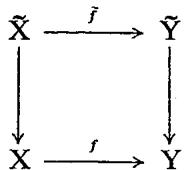
\includegraphics[keepaspectratio]{images/part001_3e847d2c.jpg}}

，并且与群 \(\{\pm1\}\) 的作用相容。

若 \(\tilde{f}\) 是 f 的一个定向，且 \(\eta\) 是 Y 的一个定向，则存在唯一一个 X 的定向 \(\xi\)，使得图表

\pandocbounded{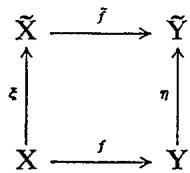
\includegraphics[keepaspectratio]{images/part001_a1f56317.jpg}}

可交换。称 \(\xi\) 由 \(\eta\) 通过 \(f\) 关联得到。

例子

\begin{enumerate}
\def\labelenumi{\alph{enumi})}
\item
  若 Y 退化为一点，则 f 的一个定向等价于 X 的一个定向。
\item
  设 \(f\) 是 étale 的。对于每个 \(x \in X\)，映射 \(\mathrm{T}_{x}(f)\) 是从 \(\mathrm{T}_{x}(\mathrm{X})\) 到 \(\mathrm{T}_{f(x)}(\mathrm{Y})\) 的同构，并通过结构转移定义一个双射
\end{enumerate}

\[
\tilde {f} _ {x}: \mathrm{Or} (\mathrm{T} _ {x} (\mathrm{X})) \rightarrow \mathrm{Or} (\mathrm{T} _ {f (x)} (\mathrm{Y})).
\]

族 \(\tilde{f}_{x}\) 定义了一个态射 \(\tilde{f}\colon\tilde{\mathbf{X}}\to\tilde{\mathbf{Y}}\)，它是 \(f\) 的一个定向，称为典范定向。

\begin{enumerate}
\def\labelenumi{\alph{enumi})}
\setcounter{enumi}{2}
\tightlist
\item
  更一般地，设 \(f\) 是浸没，并令 \(\alpha\) 为丛 T(X/Y) 的一个定向（8.1.3）。设 \(x\in X\)，且 \(\xi\) 是 \(\mathrm{T}_{x}(\mathrm{X}/\mathrm{Y})\) 的一个定向。置 \(y=f(x)\)；我们有正合序列（8.1.3）
\end{enumerate}

\[
0 \rightarrow \mathrm{T} _ {x} (\mathrm{X} / \mathrm{Y}) \rightarrow \mathrm{T} _ {x} (\mathrm{X}) \xrightarrow {\mathrm{T} _ {x} (f)} \mathrm{T} _ {y} (\mathrm{Y}) \rightarrow 0
\]

因而存在唯一一个定向 \(\tilde{f}_{\alpha}(\xi)\)，它是 \(\mathrm{T}_{y}(\mathrm{Y})\) 的定向，使得 \(\xi = \tilde{f}_{\alpha}(\xi)\alpha(x)\)（10.2.1）。映射 \(\tilde{f}_{\alpha}\colon \tilde{\mathrm{X}}\to \tilde{\mathrm{Y}}\) 是 \(f\) 的一个定向，称为与 \(\alpha\) 关联的定向。映射 \(\alpha \mapsto \tilde{f}_{\alpha}\) 是从 \(\mathrm{T}(\mathrm{X}/\mathrm{Y})\) 的定向集合到 \(f\) 的定向集合的双射。

\begin{enumerate}
\def\labelenumi{\alph{enumi})}
\setcounter{enumi}{3}
\tightlist
\item
  若 \(f: X \to Y\) 是浸入，则 \(f\) 的定向与相对于 \(f\) 的法丛的定向相对应。
\end{enumerate}

10.2.6（“乘积的定向”）。设 \(\mathbf{X}_1\)（相应地 \(\mathbf{X}_2\)）是局部有限维流形，且 \(\xi_1\)（相应地 \(\xi_2\)）是 \(\mathbf{X}_1\)（相应地 \(\mathbf{X}_2\)）的一个定向。令 \(\mathbf{X} = \mathbf{X}_1 \times \mathbf{X}_2\)。映射 \((x_1, x_2) \mapsto \xi_1(x_1)\xi_2(x_2)\)（10.2.1）是 \(\mathbf{X}_1 \times \mathbf{X}_2\) 的一个定向，称为定向 \(\xi_1\) 与 \(\xi_2\) 的乘积，记作 \(\xi_1\xi_2\) 或 \(\xi_1 \otimes \xi_2\)。

设 \(X_{i}\)（i = 1, 2）是维数为 \(n_{i}\) 的纯流形。典范同构 \(X_{1} \times X_{2} \to X_{2} \times X_{1}\) 将 \(\xi_{1} \otimes \xi_{2}\) 变为 \(\xi_{2} \otimes \xi_{1}\)（相应地变为 \(-\xi_{2} \otimes \xi_{1}\)）；若某个 \(n_{i}\) 为偶数（相应地，若 \(n_{1}\) 与 \(n_{2}\) 都为奇数）。

10.2.7（“复数情形”）。设 F 是有限维复向量空间，\(F_{R}\) 是其底层实向量空间。设 \(\{e_{1},\ldots,e_{m}\}\) 是 F 的一个基；则 \(\{e_{1},ie_{1},e_{2},ie_{2},\ldots,e_{m},ie_{m}\}\) 是 \(F_{R}\) 的一个基，而由 2m-向量定义的 \(F_{R}\) 的定向

\[
e _ {1} \wedge i e _ {1} \wedge e _ {2} \wedge i e _ {2} \wedge \dots \wedge e _ {m} \wedge i e _ {m}
\]

与 F 的基 \(\{e_{1},\ldots,e_{m}\}\) 的选取无关；这称为由给定复结构定义的 \(F_{R}\) 的定向。若 F 是两个子空间 G 与 H 的直和，则 \(F_{R}=G_{R}\oplus H_{R}\) 的定向是 \(G_{R}\) 与 \(H_{R}\) 的定向的乘积。

设 X 是一个局部有限维实流形，配备一个几乎复结构（8.8.3）。对每个 \(x \in X\)，令 \(\xi(x)\) 为其复结构定义的 \(\mathrm{T}_{x}(\mathrm{X})\) 的定向。映射 \(x \mapsto \xi(x)\) 是 X 的一个定向，称为由几乎复结构定义的定向。特别地，对于一个局部有限维复解析流形 \(X^{c}\) 的底层实解析流形 X，我们赋予它由相应几乎复结构定义的定向（8.8.6）。若把 X 上给定的复解析流形结构替换为其共轭结构（5.4.12.b)），则此定向乘以函数 \(x \mapsto (-1)^{\dim_{x} X^{c}}\)。

10.2.8. 例子

\begin{enumerate}
\def\labelenumi{\alph{enumi})}
\tightlist
\item
  设 E 是有限维实向量空间。由 E 定义的实解析流形（5.2.2）是可定向的。更确切地说，映射 \(\xi \mapsto \xi(0)\) 是从该流形的定向集合到 Or(E) 上的双射。
\end{enumerate}

特别地，流形 \(R^{n}\) 具有一个典范定向 \(\xi^{n}\)，它由半直线 \(R_{+}e_{1}\wedge\cdots\wedge e_{n}\)（属于 \(\mathrm{Or}(\mathbf{R}^{n})\)）定义。

\begin{enumerate}
\def\labelenumi{\alph{enumi})}
\setcounter{enumi}{1}
\item
  设 X 是中心为 0、半径为 \(\rho\) 的 \(\mathbf{R}^n\) 中的球面；它是 \(\mathbf{R}^n\) 的子流形。对每个 \(x \in \mathbf{X}\)，空间 \(\mathbf{T}_x(\mathbf{R}^n) = \mathbf{R}^n\) 是直线 \(\mathbf{R}x\) 与超平面 \(\mathbf{T}_x(\mathbf{X})\) 的直和。令 \(\eta_x\) 为定向 \(\mathbf{R}_+x\) 的直线 \(\mathbf{R}x\)（“向外法向”），并令 \(\xi_x\) 为 \(\mathbf{T}_x(\mathbf{X})\) 的唯一一个定向，使得 \(\eta_x\) 与 \(\xi_x\) 的乘积是定向 \(\xi^n\) 的 \(\mathbf{R}^n\)。映射 \(x \mapsto \xi_x\) 是 \(\mathbf{X}\) 的一个定向，称为典范定向。
\item
  设 X 是一个连通流形，G 是在 X 上适当地且自由地作用的离散群。X/G 可定向的充要条件是 X 可定向且 G 在 X 的定向集合上的作用是平凡的。
\item
  实射影空间 \(\mathbf{P}_{n-1}(\mathbf{R})\) 可与球面 \(S_{n-1}\) 在群 \(\{\pm1\}\) 通过 \(x\mapsto\pm x\) 的作用下的商等同；当 n 为偶数时它可定向，当 n 为奇数时它不可定向。
\item
  每个李群被连通李子群取商所得的空间都是可定向的。
\end{enumerate}

\subsection{M-扭曲微分形式}

10.3.1. 设 X 是类 \(C^{r}\) 的实流形，M 是以 X 为底空间、有限秩且类 \(C^{k}\) 的向量丛，其中 \(0 \leqslant k \leqslant r\)。令 \(\lambda_{\mathrm{M}} = (\mathrm{Or}_{\mathrm{M}}, \{\pm 1\}, \mathrm{X}, \pi)\) 为与 M 的定向流形相关的主纤维化（10.2.2）。令结构群 \(\{\pm 1\}\) 通过乘法作用于 R。我们把 \(\tilde{R}_{M}\) 记作与 \(\lambda_{M}\) 相关的、纤维类型为 R 的丛（赋予上文定义的运算律）（6.5.1）；它带有（7.10.2）一个以 X 为底、秩为 1 且类 \(C^{k}\) 的向量丛结构；称为 M-扭曲标量丛。

10.3.2. 我们有一个交换图：

\pandocbounded{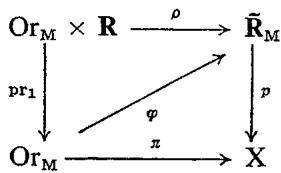
\includegraphics[keepaspectratio]{images/part001_9c73fb1b.jpg}}

其中 \(p\) 表示 \(\tilde{\mathbf{R}}_{\mathbf{M}}\) 到 \(\mathbf{X}\) 的典范投影，\(\rho\) 表示 \(\tilde{\mathbf{R}}_{\mathbf{M}}\) 的标架映射（6.5.1），并且有 \(\varphi(\xi) = \rho(\xi, 1)\)，其中 \(\xi \in \mathrm{Or}_{\mathbf{M}}\)。特别地，丛 \(\tilde{\mathbf{R}}_{\mathbf{M}}\) 在 \(\pi\) 下的逆像可与平凡丛 \(\mathrm{Or}_{\mathbf{M}} \times \mathbf{R}\) 等同。还将 \(\xi\)（\(\mathrm{Or}_{\mathbf{M}}\) 中的元素）与其在 \(\tilde{\mathbf{R}}_{\mathbf{M}}\) 中的像通过 \(\varphi\) 等同；按照这一约定，有 \(\rho(\xi, a) = a\xi\)（对所有 \((\xi, a) \in \mathrm{Or}_{\mathbf{M}} \times \mathbf{R}\)）；有 \(a\xi = b\eta\) 当且仅当存在 \(e \in \{\pm 1\}\) 使得 \(b = ea\) 且 \(\eta = e\xi\)。因此，\(\xi\) 是 \(\mathbf{M}\) 的一个定向，定义了截面 \(x \mapsto \xi(x)\)，它取值于 \(\tilde{\mathbf{R}}_{\mathbf{M}}\)。

存在唯一一个同构 \(j\)，它从 \(\tilde{\mathbf{R}}_{\mathbf{M}} \otimes \tilde{\mathbf{R}}_{\mathbf{M}}\) 到平凡丛 \(\mathbf{R}_{\mathbf{x}} = \mathbf{X} \times \mathbf{R}\)，使得 \(j(\xi \otimes \xi) = (\pi(\xi), 1)\) 对所有 \(\xi \in \mathrm{Or}_{\mathbf{M}}\) 成立；借此可将向量丛 \(\tilde{\mathbf{R}}_{\mathbf{M}}\) 与其对偶等同。

10.3.3. 设 F 还是以底空间 X 为基底、类 \(C^{r-1}\) 的向量丛。X 上取值于 \(\tilde{R}_{M} \otimes F\) 的微分形式称为取值于 F 的 M-扭曲微分形式。此类 p 次形式是丛 \(\operatorname{Alt}^{p}(\mathrm{T}(\mathrm{X}); \tilde{\mathbf{R}}_{\mathbf{M}} \otimes \mathbf{F})\) 的截面，并以显然的方式将其与 \(\tilde{R}_{M} \otimes \operatorname{Alt}^{p}(\mathrm{T}(\mathrm{X}); \mathbf{F})\) 等同。当 F 是由 Banach 空间 E 定义的平凡丛时，简称为取值于 E 的 M-扭曲形式；当 E = C（相应地 R）时，称为复 M-扭曲形式（相应地称为实 M-扭曲形式，或 M-扭曲形式）。

设 \(\omega\) 是取值于 F 的 M-扭曲形式，次数为 \(p\)。由于 \(\pi\colon\mathrm{Or}_{\mathbb{M}}\to\mathbf{X}\) 是 étale 的，且 \(\pi^{*}(\tilde{\mathbf{R}}_{\mathbb{M}})=\mathrm{Or}_{\mathbb{M}}\times\mathbf{R}\)，所以可以将 \(\pi^{*}(\tilde{\mathbf{R}}_{\mathbb{M}}\otimes\operatorname{Alt}^{p}(\mathrm{T}(\mathrm{X});\mathrm{F}))\) 与 \(\mathrm{Alt}^{p}(\mathrm{T}(\mathrm{Or}_{\mathbb{M}});\pi^{*}(\mathrm{F}))\) 等同，而 \(\omega\) 定义了 \(\tilde{\omega}\)（7.4.3）作为 \(\mathrm{Alt}^{p}(\mathrm{T}(\mathrm{Or}_{\mathbb{M}});\pi^{*}(\mathrm{F}))\) 的截面，换言之，是次数为 \(p\)、定义在 \(\mathrm{Or}_{\mathbb{M}}\) 上且取值于 \(\pi^{*}(\mathrm{F})\) 的微分形式。由此得到一个双射，从 X 上取值于 F 的 M-扭曲形式空间（次数为 \(p\)）到形式空间：其中 \(\tilde{\omega}\) 是次数为 \(p\)、定义在 \(\mathrm{Or}_{\mathbb{M}}\) 上且取值于 \(\pi^{*}(\mathrm{F})\) 的形式，且满足

\[
\tilde{\omega}(-\xi)=-\tilde{\omega}(\xi)\quad\text{对每个 }\xi\in\mathrm{Or}_{\mathbb{M}}.
\]

当 M 配备一个定向 \(\xi\) 时，映射 \(\omega \mapsto \xi \otimes \omega\) 使得可以将 \(\mathrm{Alt}^p(\mathrm{T}(\mathrm{X});\mathrm{F})\) 的截面（换言之，\(p\) 次通常微分形式）与取值于 F 的 \(p\) 次 M-扭曲形式等同。

10.3.4. 设 \(\omega\) 是 X 上取值于 Banach 空间 E、次数为 \(p\) 且类为 \(\mathbf{C}^s\) 的 M-扭曲微分形式（\(1 \leqslant s \leqslant \inf(k, r - 1)\)）。存在唯一一个 M-扭曲微分形式 \(d\omega\)，次数为 \(p + 1\)，取值于 E，且满足：对于 X 的每个开集 U、每个定向 \(\xi\)，属于 \(M|_{U}\) 的，以及 U 上的每个微分形式 \(\alpha\)，若 \(\omega|_{U} = \xi \otimes \alpha\)，则 \(d\omega|_{U} = \xi \otimes d\alpha\)。形式 \(d\omega\) 属于类 \(\mathbf{C}^{s-1}\)；称为 \(\omega\) 的外微分。

若将 \(\tilde{\omega}\)（相应地 \(\widetilde{d\omega}\)）记作 \(\mathrm{Or}_{\mathbb{M}}\) 上与 \(\omega\)（相应地与 \(d\omega\)）对应的微分形式，如 10.3.3 中那样，则有 \(d(\tilde{\omega}) = \widetilde{d\omega}\)。

若 \(\zeta\) 是类为 \(\mathbf{C}^s\) 的向量场，定义在 \(X\) 上，则以类似方式定义 M-扭曲形式 \(\theta_{\zeta}.\omega\)。有

\[
\theta_ {\zeta}. \omega = d (i (\zeta) \omega) + i (\zeta) d \omega
\]

并且 \(\theta_{\zeta}.\omega\) 属于类 \(\mathbf{C}^{s - 1}\)。

\subsection{与扭曲微分形式相关的测度}

回顾一下，在本节中，我们假定 K = R，且所考虑的所有流形都是局部有限维的。

10.4.1. 设 X 是类 \(C^{r}\) 的流形。取切丛 T(X) 作为向量丛 M，便可应用 10.3 的定义和结果。于是有 \(\mathrm{Or}_{\mathbf{M}} = \tilde{\mathbf{X}}\)（10.2.4）；我们将其记作 \(\tilde{\mathbf{R}}_{\mathbf{X}}\)，并将扭曲标量丛简单地称为丛 \(\tilde{\mathbf{R}}_{\mathrm{T}(\mathbf{X})}\)（10.3.1）\footnote{注意，当把 X 看作自身上秩为 0 的向量丛结构时，这一记号与 \(\widetilde{\mathbf{R}}_{\mathbf{M}}\) 的记号冲突。}；取值于向量丛 F 的 T(X)-扭曲微分形式简单地称为取值于 F 的扭曲（或奇）微分形式。当 X 配备一个定向时，映射 \(\omega \mapsto \xi \otimes \omega\) 使得可以将通常微分形式（有时称为“偶”微分形式）与扭曲形式等同。

10.4.2. 设 \(f\colon\mathbf{X}\to\mathbf{Y}\) 是类 \(\mathbf{C}^{r}\) 流形的态射，且 \(\tilde{f}\colon\tilde{\mathbf{X}}\to\tilde{\mathbf{Y}}\) 是 \(f\) 的一个定向（10.2.5）。存在唯一一个同构 \(j\)，从 \(f^{*}(\widetilde{\mathbf{R}}_{\mathbf{Y}})\) 到 \(\widetilde{\mathbf{R}}_{\mathbf{X}}\)，使得 \(\tilde{x}=j(\pi(\tilde{x}),\tilde{f}(\tilde{x}))\) 对所有 \(\tilde{x}\in\tilde{\mathbf{X}}\) 成立。我们通过 \(j\) 将这两个丛等同。若 \(\omega\) 是 Y 上取值于向量丛 F 的扭曲形式，次数为 \(p\)，则逆像 \(f^{*}(\omega)\) 可与 X 上次数为 \(p\)、取值于 \(f^{*}(\mathrm{F})\) 的扭曲微分形式等同。若将 \(\tilde{\omega}\)（相应地 \(\widetilde{f^{*}(\omega)}\)）记作分别位于 \(\tilde{\mathbf{Y}}\)（相应地 \(\tilde{\mathbf{X}}\)）上、与 \(\omega\)（相应地 \(f^{*}(\omega)\)）对应的微分形式，如 10.3.3 中那样，则有 \(\tilde{f}^{*}(\tilde{\omega})=\widetilde{f^{*}(\omega)}\)。

当 F 是由 Banach 空间定义的平凡丛时，运算 \(f^*\) 与外微分交换（10.3.4）。

10.4.3. 设 X 是维数为 n 的纯流形，\(\omega\) 是 X 上取值于 Banach 空间 E 的 n 次扭曲微分形式。令 \(c = (\mathrm{U}, \varphi, \mathbf{R}^{n})\) 为 X 的一个图，令 \(\xi^{n}\) 为 \(R^{n}\) 的典范定向；以 \(u^{1}, \ldots, u^{n}\) 表示 \(R^{n}\) 上的坐标函数。存在唯一一个函数 \(f_{c}\)，定义在 \(\varphi(\mathrm{U})\) 上，取值于 E，使得

\[
\omega | \mathrm{U} = \varphi^ {*} (\xi^ {n} \otimes f _ {c}. d u ^ {1} \wedge \dots \wedge d u ^ {n}).
\]

称 \(\omega\) 是局部可积的，如果对于 X 的每个图 \(c = (\mathrm{U},\varphi ,\mathbb{R}^n)\)，相应函数 \(f_{c}\) 关于 \(\lambda_{\varphi (\mathrm{U})}^{\otimes n}\) 局部可积（其中 \(\lambda\) 表示 R 上的勒贝格测度）。假定这一点成立且 X 是分离的。在 X 上存在一个取值于 E 的向量测度 \(\alpha (\omega)\)，并且唯一地具有如下性质：对于 X 的每个图 \(c = (\mathrm{U},\varphi ,\mathbb{R}^n)\)，其在 \(\varphi\) 下的像，即测度 \(\alpha (\omega)\) 在 U 上的限制，是测度 \(f_{c}\lambda_{\varphi(\mathrm{U})}^{\otimes n}\)（INT, VI, § 2, no. 4）。称 \(\alpha (\omega)\) 为由 \(\omega\) 定义的测度，并且通常仍简记为 \(\omega\)。\(\alpha (\omega)\) 的支集包含于 \(\operatorname{Supp}\omega\)（\(\omega\) 的支集）中（把微分形式 \(\omega\) 的支集定义为满足 \(x\in X\) 且 \(\omega (x)\neq 0\) 的 x 的集合的闭包）。

若 \(f\) 是 X 上关于测度 \(\alpha(\omega)\) 局部可积的实函数，则微分形式 \(f\omega\) 局部可积，且有 \(\alpha(f\omega) = f.\alpha(\omega)\)。

若 \(g\) 是 X 上关于 \(\alpha(\omega)\) 本质可积的实函数，则其积分通常记作 \(\int_{\mathbf{X}} g\omega\)、\(\int g\omega\) 或 \(\int g(x)\omega(x)\)；人们避免将其记作 \(\int g d\omega\)，因为这可能与 \(d\omega\)（\(\omega\) 的外微分）混淆；当 \(\omega\) 属于类 \(C^{1}\) 时，该外微分有定义（并且还等于 0）。若 A 是 X 的一个子集，且其示性函数 \(\varphi_{\mathrm{A}}\) 关于 \(\alpha(\omega)\) 本质可积，则 \(\varphi_{\mathrm{A}}\) 的积分记作 \(\int_{A} \omega\)。若常数 1 关于 \(\alpha(\omega)\) 本质可积，则称 \(\omega\) 是可积的。

现在令 \(p\) 为整数，满足 \(0 \leqslant p \leqslant n\)，令 \(\omega\) 为 X 上取值于 Banach 空间 E、次数为 \(p\) 的扭曲微分形式。此外，令 Y 为 X 的一个维数为 \(p\) 的纯子流形；假设典范嵌入 \(i: Y \to X\) 配备了一个定向。于是，其逆像 \(i^{*}(\omega)\)（10.4.2）有时记作 \(\omega|Y\)。若 \(\omega|Y\) 可积，置

\[
\int_ {\mathbf {Y}} \omega = \int_ {\mathbf {Y}} \omega | \mathbf {Y}.
\]

10.4.4. 设 X 是一个配备定向 \(\xi\) 的 n 维纯流形。通常微分形式与扭曲微分形式之间的等同 \(\omega \mapsto \xi \otimes \omega\) 使得可以将前述结果应用于 X 上的 n 次形式；因此，每个局部可积的 n 次形式 \(\omega\) 都关联着 X 上的一个测度，仍记作 \(\omega\)。若 E = R，则这样的形式 \(\omega\) 局部具有可积模（10.1.5），与其对应的测度 \(\text{mod}(\omega)_{\mu}\)（10.1.6）恰好是 \(|\omega|\)（测度 \(\omega\) 的绝对值）（INT, III, § 1, no. 6）。

10.4.5. 例。--- 设 X 是一个定向的、分离的 1 维纯实流形，且 \(z: \mathrm{X} \to \mathbf{C}\) 是从 X 到 C 的可微映射。复微分形式 \(dz\) 在 X 上定义了一个也记作 \(dz\) 的复测度。这尤其适用于 X 是 C 的一个 1 维纯可微子流形、\(z\) 是 X 到 C 的嵌入的情形。

更具体地，设 X 是中心为 0、半径 \(\rho > 0\) 的圆；按照 10.2.8 b) 中的指示，并利用 C 与 \(\mathbf{R}^2\) 的通常等同，为 X 赋予定向。若 \(x \in \mathbf{X}\)，切空间 \(\mathrm{T}_x(\mathbf{X})\) 可与 \(\mathbf{R}ix\) 等同，后者是 \(\mathrm{T}_x(\mathbf{C}) = \mathbf{C}\) 中的直线，而所选定向是半直线 \(\mathbf{R}_+ix\)。若 \(f\) 是 X 上取值于复 Banach 空间的连续函数，则 \(f\) 关于测度 \(dz\) 的积分由公式给出

\[
\int_ {\mathbb {X}} f (z) d z = i \rho \int_ {0} ^ {2 \pi} f (\rho e ^ {i \alpha}) e ^ {i \alpha} d \alpha .
\]

例如，若 \(n\) 是一个整数，则有

\[
\int_ {\mathrm{X}} z ^ {n} d z = i \rho^ {n + 1} \int_ {0} ^ {2 \pi} e ^ {(n + 1) i \alpha} d \alpha = \left\{ \begin{array}{l l} 0 & \quad \text {if } n \neq - 1 \\ 2 i \pi & \quad \text {if } n = - 1. \end{array} \right.
\]

10.4.6（“复数情形”）。设 \(X^{c}\) 是一个分离的、纯维数为 \(m\) 的复解析流形，且 \(\omega\) 是次数为 \(m\) 的全纯微分形式，定义在 \(X^{c}\) 上。设 X 是 \(X^{c}\) 的底层实解析流形；形式 \(\omega\) 与 X 上的 \((m,0)\) 型形式等同（8.8.9）；令 \(\overline{\omega}\) 为其共轭（8.8.2）。形式 \(i^{m^{2}}\omega \wedge \overline{\omega}\) 是 X 上次数为 \(2m\) 的实微分形式；考虑到 X 的典范定向（10.2.7），此形式与 X 上的一个测度等同，而该测度正是 10.1.6 中定义的正测度 \(\operatorname{mod}(\omega)_{\mu}\)，其中 \(\mu\) 是由微分形式 \(i \, dz \wedge \overline{dz}\) 定义的测度，换言之，是测度 \(\lambda^{\otimes 2}\) 在 \(\mathbf{C}\) 上的两倍（按通常方式与 \(\mathbf{R}^{2}\) 等同）。

令 H 为由全纯形式 \(\omega\)（次数为 \(m\)，定义在 \(\mathbf{X}^c\) 上）组成的空间，使得测度 \(\omega \wedge \overline{\omega}\) 有界。对于 H 中的 \(\alpha, \beta\)，复测度 \(\alpha \wedge \overline{\beta}\) 有界；令

\[
(\alpha | \beta) = i ^ {m ^ {2}} \int_ {\mathbf {X}} \alpha \wedge \bar {\beta},
\]

从而得到 H 上的一个厄米形式，它使 H 成为 Hilbert 空间。

\section{Stokes 公式}

本段中，我们假定 K = R。

\subsection{片段}

11.1.1. 设 E 是 Banach 空间。如果存在连续线性泛函 \(h \neq 0\) 和实数 k 使得 \(S = \{x|h(x) \leqslant k\}\)，则 E 的子集 S 称为闭半空间（参见 EVT, II, §2, no. 6）；此时 S 的边界是闭超平面 \(\{x|h(x) = k\}\)；它也称为 S 的边界，记作 \(\partial S\)。

11.1.2. 设 X 是类 \(C^{r}\) 流形，A 是 X 的一个子集。如果对每个 \(a \in A\)，都存在 X 在 a 处的图 \(c = (U, \varphi, E)\)，使得 \(\varphi(A \cap U)\) 是 E 的某个闭半空间的开子集，则称 A 是 X 的一个片段。置 \(\partial A = A - \mathring{A}\)（A 的非内部点的集合）。它是 A 的子流形，称为 A 的边界。\footnote{这一术语源于以下事实：A 自然地带有一个“带边界的流形”结构，其边界为 \(\partial A\)。关于这一范畴的定义，以及更一般的“带角流形”范畴，读者可参阅 H. Cartan, \emph{Séminaire 1961/62, Topologie Différentielle}, lectures 1–2–3（A. Douady），Benjamin, New York, 1969。需要指出的是，可以证明，每个边界为仿紧的“带边界流形”都同构于某个流形的闭片段。}若 \(a \in \partial A\)，则存在 X 在 a 处、以 a 为中心的图 \(c = (U, \varphi, E)\) 以及 E 的闭超平面 H，使得 \(\varphi(A \cap U)\) 是由 H 定义的 E 的某个闭半空间 \(S_{c}\) 中 0 的一个开邻域（EVT, II, § 2, no. 6），并且 \(\varphi(\partial A \cap U) = H \cap \varphi(A \cap U)\)。这样的图称为 A 在 a 处的适配图。于是，闭半空间 \(S_{c}\) 是使 \(\varphi(A \cap U)\) 成为开集的唯一 E 的闭半空间。

对于 X 的一个闭子集 A，它成为 X 的片段的充要条件是：\(\mathring{A}\) 在 A 中稠密，并且 \(A-\mathring{A}\) 在其每一点处都是 X 的余维 1 子流形。

11.1.3. 例子

\begin{enumerate}
\def\labelenumi{\alph{enumi})}
\item
  在 \(\mathbf{R}^{n}\) 中，半径 \(>0\) 的闭球是一个片段；其边界是相应的球面。
\item
  若 A 是流形 X 的一个片段，且 B 是 \(\partial A\) 的闭子集，则 A - B 是 X 的一个片段。
\item
  设 \(\varphi: X \to X'\) 是类 \(C^r\) 的流形态射，且 \(A'\) 是 \(X'\) 的一个片段。若 \(\varphi\) 与 \(\partial A'\) 横截（5.11.6），则 \(\varphi^{-1}(A')\) 是 \(X\) 的一个片段，其边界为 \(\varphi^{-1}(\partial A')\)。
\end{enumerate}

特别地，设 \(h: \mathbf{X} \to \mathbf{R}\) 是类 \(\mathbf{C}^r\) 的函数，且 \(a \in \mathbf{R}\)；假定不存在 \(x \in \mathbf{X}\) 使得 \(h(x) = a\) 且 \(d_x h = 0\)。集合 \(\{x | h(x) \leqslant a\}\) 是 \(\mathbf{X}\) 的一个闭片段，其边界为 \(h^{-1}(a)\)。

\begin{enumerate}
\def\labelenumi{\alph{enumi})}
\setcounter{enumi}{3}
\tightlist
\item
  若 \(r = \infty\) 且 X 局部紧，则 X 的每个紧子集都有一个由紧片段组成的邻域基本系。
\end{enumerate}

11.1.4. 设 X 是类 \(\mathbf{C}^{\mathrm{r}}\) 的流形，A 是 X 的一个片段。设 \(a \in \partial \mathrm{A}\)，\(v \in \mathrm{T}_a(\mathrm{X})\)。令 \(c = (\mathrm{U}, \varphi, \mathrm{E})\) 为 A 在 \(a\) 处的适配图（11.1.2），并令 \(h = \theta_c^{-1}(v)\) 为 E 中与 \(v\) 对应的元素（5.5.1）。令 \(\mathrm{S}_c\) 为 E 的闭半空间，使得 \(\varphi(\mathrm{A} \cap \mathrm{U})\) 是其开子集（11.1.2）。称 \(v\) 是 A 在 \(a\) 处的向内（相应地严格向内、向外、严格向外）向量，当且仅当 \(h\) 属于 \(\mathrm{S}_c\)（相应地属于 \(\dot{\mathrm{S}}_c\)、\(-\mathrm{S}_c\)、\(-\dot{\mathrm{S}}_c\)）；这个条件与适配图 \(c\) 的选择无关。我们把 \(\mathrm{T}_a^+(\mathrm{A})\)（相应地 \(\mathrm{T}_a^-(\mathrm{A})\)）记作 A 的向外（相应地向内）向量在 \(\mathrm{T}_a(\mathrm{X})\) 中的集合。这些是 \(\mathrm{T}_a(\mathrm{X})\) 的闭半空间，其边界包含 0。于是有

\[
\mathrm{T} _ {a} (\partial \mathrm{A}) = \mathrm{T} _ {a} ^ {+} (\mathrm{A}) \cap \mathrm{T} _ {a} ^ {-} (\mathrm{A}).
\]

\subsection{片段的 Stokes 公式}

本节中，X 表示类 \(C^{r}\)（\(r \geqslant 2\)）的纯有限维分离流形。A 表示 X 的一个片段，i 表示将 \(\partial A\) 典范嵌入 X 的映射。E 表示 Banach 空间。

11.2.1. 设 \(x \in \partial A\)，且 \(\xi\) 是 \(T_x(\partial A)\) 的一个定向；把 \(\tilde{i}_x(\xi)\) 记作 \(T_x(X)\) 的一个定向，其中含有元素 \(v \wedge u\)，这里 \(v\) 是 A 在 x 处的严格向外向量（11.1.4），而 \(u\) 是 \(\bigwedge^{n-1} T_x(\partial A)\) 中属于定向 \(\xi\) 的非零元素。映射 \(\tilde{i}_x\) 是从 \(\text{Or}(T_x(\partial A))\) 到 \(\text{Or}(T_x(X))\) 的双射。对于映射 \(\tilde{i}_x\)（\(x \in \partial A\)），它定义了一个态射 \(\tilde{i} \colon \partial \widetilde{A} \to \widetilde{X}\)，它是 \(i\) 的一个定向（10.2.5）。若 \(\xi\) 是 X 的一个定向，则 \(\partial A\) 的定向与 \(\xi\) 相关联，并由 \(\tilde{i}\) 得到（10.2.5），称为由 \(\xi\) 定义的定向。

例。--- 当 \(X = R^{n}\) 时，\(\xi\) 是 \(R^{n}\) 的通常定向，且 A 是半径 \(\rho>0\) 的闭球；球面 \(\partial A\) 的定向由 \(\xi\) 定义，就是典范定向（10.2.8, b)）。

11.2.2. 设 \(\omega\) 是 X 上取值于 Banach 空间 E 的 \(p\) 次扭曲微分形式（10.4.1）；其逆像 \(i^{*}(\omega)\) 是 \(\omega\) 通过有向态射 \(i\colon\partial A\to X\) 得到的逆像，记作 \(\omega|\partial A\)，称为 \(\omega\) 在 \(\partial A\) 上诱导的形式（参见 10.4.3）。

11.2.3. 我们作如下两个假设之一：

\begin{enumerate}
\def\labelenumi{(\roman{enumi})}
\tightlist
\item
  \(\omega\) 是 X 上取值于 E 的 \(n - 1\) 次扭曲微分形式；
\item
  X 是有向的，\(\partial A\) 配备与之相应的定向（11.2.1），且 \(\omega\) 是 X 上取值于 E 的 \(n - 1\) 次微分形式。
\end{enumerate}

进一步假设 \(\omega\) 属于类 \(C^{1}\)，且 A 与 \(\omega\) 的支集的交是紧的。\(d\omega\) 是 \(\omega\) 的外微分，并且连续（8.3.5 和 10.3.4）。

A 的示性函数关于 X 上由 \(d\omega\) 定义的向量测度是本质可积的，而 \(\omega|\partial\mathrm{A}\) 是 \(n-1\) 次定义在 \(\partial\mathrm{A}\) 上的微分形式，并且可积（10.4.3 和 10.4.4）。有

\[
\int_ {\mathrm{A}} d \omega = \int_ {\partial \mathrm{A}} \omega \quad (\text{Stokes公式})
\]

11.2.4. 设 \(\alpha\) 是 X 上取值于 Banach 空间 E、具有紧支集、次数为 \(n\) 且类为 \(\mathbf{C}^1\) 的扭曲微分形式。若存在 X 上取值于 E、具有紧支集的扭曲微分形式 \(\omega\)，其次数为 \(n - 1\) 且类为 \(\mathbf{C}^1\)，使得 \(\alpha = d\omega\)，则必须有 \(\int_{\mathbb{X}} \alpha = 0\)。若 X 连通，则此条件充分；此外，若 \(\alpha\) 属于类 \(\mathbf{C}^k\)（\(k\leqslant r-1,\ k\neq\omega\)），则可以选取 \(\omega\) 为类 \(\mathbf{C}^k\)。

11.2.5. 假设 X 是 \(\mathbf{C}\) 的底层实流形，E 是复 Banach 空间，A 是 X 的一个紧片段。赋予 X 由其复结构定义的定向（10.2.7）。设 f 是从 A 到 E 的连续映射，且其在 A 的内部 \(\mathring{A}\) 上的限制是全纯的。以 \(dz\) 表示嵌入 \(z\colon\partial A\to\mathbf{C}\) 的微分。形式 \(f\cdot dz\)，即 f 与 dz 的乘积，是 \(\partial A\) 上取值于 E 的 1 次微分形式，属于类 \(C^{0}\)，并且有：

\[
\int_ {\partial \mathbf {A}} f\, d z = 0 \quad (\text{Cauchy公式})
\]

当 \(f\) 可延拓为定义在 A 的某个开邻域 U 上、仍记作 \(f\) 的全纯映射时，形式 \(f.dz\)（此时 z 表示 U 到 \(\mathbf{C}\) 的典范嵌入）在 U 上属于类 \(C^{\omega}\)，且其外微分为零。

11.2.6（“积分的导数”）。假设 X 是有向的。设 Y 是类 \(C^{r}\) 的流形，\(\alpha\) 是 Y 上取值于 E、具有紧支集、次数为 \(n\)、类为 \(C^{1}\) 的微分形式。设 I 是包含 0 的 R 的开子集，\(g: I \times X \to Y\) 是类 \(C^{r}\) 的态射；对于 \(t \in I\)，记 \(g_{t}\) 为从 X 到 Y 的映射 \(x \mapsto g(t, x)\)。令 \(\psi\) 为从 X 到 T(Y) 的态射，由 \(\psi(x) = T_{(0,x)}(g)(1,0)\) 定义；它是 \(g_{0}\) 的一个提升（8.6.5）。假设 \(\operatorname{pr}_{1}\colon I\times A\to I\) 限制在 \(I\times A\) 与 \(g^{*}(\alpha)\) 的支集的交集上是本原的（TG, I, § 10）。则对于每个 \(t \in I\)，A 与 \(g_{t}^{*}(\alpha)\) 的支集的交是紧的；映射 \(t \mapsto \int_{A} g_{t}^{*}(\alpha)\) 在 I 上属于类 \(C^{1}\)，且其在原点处的导数由公式给出

\[
\frac {d}{d t} \left(\int_ {\mathrm{A}} g _ {t} ^ {*} (\alpha)\right) _ {t = 0} = \int_ {\mathrm{A}} \theta_ {\psi}. \alpha = \int_ {\mathrm{A}} i (\psi) d \alpha + \int_ {\partial \mathrm{A}} i (\psi) \alpha ,
\]

参见第 8.6 号。

\subsection{局部多面体集的 Stokes 公式}

本号中，X 表示类 \(C^{r}\)（\(r \geqslant 2\)）的有限维纯实流形；我们假定 X 是分离的。\footnote{读者若对更一般的情形感兴趣，可参阅 H. Whitney, \emph{Geometric Integration Theory}, 第 III 章 § 18（Princeton Univ. Press, 1957）。}

11.3.1. 设 A 是有限维实向量空间的一个子集。如果 A 是有限个闭半空间的有限交的并，则称 A 是多面体的。

称 X 的子集 A 是局部多面体的，如果对于每个 \(x \in X\)，都存在 X 在 x 处的图 \(c = (\mathrm{U}, \varphi, \mathrm{E})\) 以及 E 的一个多面体子集 \(A_{c}\)，使得 \(\varphi(\mathrm{A} \cap \mathrm{U}) = \varphi(\mathrm{U}) \cap \mathrm{A}_{c}\)。X 的一个片段是局部多面体子集。

11.3.2. 设 A 是 X 的闭子集，令 \(\mathrm{Fr}(\mathrm{A}) = \mathrm{A} - \mathring{\mathrm{A}}\) 为其边界。称 \(x \in \mathrm{Fr}(\mathrm{A})\) 为正则点，如果存在 x 的一个开邻域 U，使得 \(A \cap U\) 是流形 U 的一个片段（此时 x 属于 \(A \cap U\) 的边界）。我们把 \(\partial A\) 记作 \(\mathrm{Fr}(\mathrm{A})\) 的正则点集合，并称其为 A 的正则边界（或简称边界）。集合 \(A' = \mathring{A} \cup \partial A\) 是 X 的一个片段，其边界为 \(\partial A\)。

11.3.3. * 例。--- 设 \(\mathcal{H}\) 是维数为 \(n\) 的有限维实仿射空间 E 中的一个局部有限超平面集，C 是相对于 \(\mathcal{H}\) 的 E 的一个室（LIE, V, § 1, no. 3）。C 的闭包 \(\overline{\mathbf{C}}\) 是流形 E 的局部多面体子集；\(\overline{\mathbf{C}}\) 的正则边界是 C 的各个面的并（同上，no. 4）。特别地，若 C 是一个开单纯形（同上，no. 6），顶点为 \(a_0, \ldots, a_n\)，则 \(\overline{\mathbf{C}}\) 的边界是各个 \(\overline{\mathbf{C}_{\{i\}}}\)（\(0 \leqslant i \leqslant n\)）的并，其中 \(\mathbf{C}_{\{i\}}\) 是由顶点 \(a_0, \ldots, a_{i-1}, a_{i+1}, \ldots, a_n\) 在这些顶点生成的仿射空间中的开单纯形。*
11.3.4. 设 A 是 X 的局部多面体子集，\(\omega\) 是 X 上取值于 Banach 空间 E 的 \(n - 1\) 次扭曲微分形式；假设 \(\omega\) 属于类 \(\mathbf{C}^1\)，且其支集与 A 的交是紧的。于是，A（相应地 \(A'\)、\(\mathring{A}\)）的示性函数关于 X 上由 \(d\omega\) 定义的向量测度都是本质可积的，并且有

\[
\int_ {\mathrm{A}} d \omega = \int_ {\mathrm{A} ^ {\prime}} d \omega = \int_ {\mathring{\mathrm{A}}} d \omega.
\]

形式 \(\omega|\partial\mathbf{A}\)（对于 \(\partial\mathbf{A}\) 的典范嵌入所带的典范定向，该嵌入被看作片段 \(\mathbf{A}'\) 的边界并嵌入 \(\mathbf{X}\)）在 \(\partial\mathbf{A}\) 上可积，并且有

\[
\int_ {\mathbf {A}} d \omega = \int_ {\partial \mathbf {A}} \omega \quad (\text{Stokes公式}).
\]

当 X 配备一个定向、\(\partial\mathbf{A}\) 配备相应的定向（11.2.1）时，如果 \(\omega\) 是 X 上取值于 E 的 \(n-1\) 次普通微分形式、属于类 \(\mathbf{C}^{1}\)，且 \(\mathbf{A}\cap\operatorname{Supp}\omega\) 是紧的，则此公式仍然成立。

\subsection{相对 Stokes 公式（沿纤维积分）}

本号中，X 和 S 表示两个类 \(C^{r}\) 的（实）流形，且 \(\pi: X \to S\) 是一个浸没。我们记 n 为一个整数，并假定对于每个 \(s \in S\)，纤维 \(X_{s} = \pi^{-1}(s)\) 是 \(\pi\) 在 s 处的纤维（它是 X 的子流形（5.10.5）），都是纯 n 维的。

11.4.1. 设 E 和 H 是两个向量空间，F 是 H 的一个 n 维有限维向量子空间。

令 p 为一个满足 \(\geqslant0\) 的整数，令 u 为一个交错的 \((n+p)\)-线性映射，从 \(H^{n+p}\) 到 E，令 \(t_{1},\ldots,t_{p}\) 为 \(H/F\) 的元素；令 \(t_{1}^{\prime},\ldots,t_{p}^{\prime}\) 为 \(t_{1},\ldots,t_{p}\) 在 H 中的代表元。映射

\[
(x _ {1}, \dots , x _ {n}) \mapsto u (t _ {1} ^ {\prime}, \dots , t _ {p} ^ {\prime}, x _ {1}, \dots , x _ {n})
\]

是从 \(\mathbf{F}^n\) 到 E 的 n-线性交错映射，它只依赖于 u 和 \(t_i\)；记作 \(u \perp (t_1, \ldots, t_p)\)（对于特殊情形 \(\mathbf{E} = \mathbf{K}\)，参见 A, III, p. 158）。映射

\[
\left(t _ {1}, \dots , t _ {p}\right) \mapsto u \perp \left(t _ {1}, \dots , t _ {p}\right)
\]

是 p-线性交错的。

11.4.2（“\(\pi\)-扭曲”）。考虑 X 上的向量丛 \(\mathrm{T}(\mathrm{X}/\mathrm{S})\)（8.1.3）；它在 X 的每一点处都有有限秩 n。置 \(\tilde{R}_{\pi} = \tilde{R}_{T(X/S)}\)（10.3.1），\(\tilde{X}_{\pi} = \mathrm{Or}_{T(X/S)}\)（10.2.2）。设 \(s \in S\)；利用 \(\mathrm{T}(\mathrm{X}/\mathrm{S})|_{\mathbf{X}_{s}}\) 与 \(\mathrm{T}(\mathbf{X}_{s})\) 的自然等同（8.1.3），复合映射 \(\tilde{\pi}: \tilde{X}_{\pi} \to S\)（它是 \(\pi\) 与典范映射 \(\tilde{X}_{\pi} \to X\) 的复合）在 s 处的纤维是 \(\tilde{X}_{s}\)（10.2.4）。X 上的 \(\pi\)-扭曲微分形式称为 \(\mathrm{T}(\mathrm{X}/\mathrm{S})\)-扭曲微分形式（10.3.3）。

11.4.3（“S-态射的 S-定向”）。设 \(\mathbf{X}'\) 是一个配备浸没 \(\pi'\colon\mathbf{X}'\to\mathbf{S}\) 的簇，其纤维 \(\mathbf{X}'_{s}\) 都是纯有限维 \(n'\) 维的；设 \(\varphi\colon\mathbf{X}'\to\mathbf{X}\) 是满足 \(\pi'=\pi\circ\varphi\) 的态射。一个 \(\varphi\) 的 S-定向是态射 \(\tilde{\varphi}\colon\tilde{\mathbf{X}}'_{\pi'}\to\tilde{\mathbf{X}}_{\pi}\)，它与群 \(\{\pm1\}\) 的作用交换，并使图表可交换。

\pandocbounded{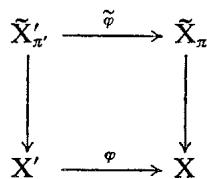
\includegraphics[keepaspectratio]{images/part001_c0391fc0.jpg}}

为 \(\varphi\) 配备 S-定向的数据使得可以像在 10.4.2 中那样，将丛 \(\tilde{\mathbf{R}}_{\pi'}\) 与 \(\varphi^{*}(\tilde{\mathbf{R}}_{\pi})\) 等同，并定义对 \(\pi\)-扭曲微分形式通过 S-定向态射 \(\varphi\) 的拉回；它是 \(\pi'\)-扭曲微分形式，定义在 \(\mathbf{X}'\) 上。

11.4.4. 设 A 是 X 的一个片段，使得 \(\pi\) 在 \(\partial\mathbf{A}\) 上的限制是浸没。对每个 \(s\in\mathbf{S}\)，纤维 \(\mathbf{X}_{s}=\pi^{-1}(s)\) 是与 \(\partial\mathbf{A}\) 横截的 X 的子流形，而 \(\mathbf{A}\cap\mathbf{X}_{s}\) 是 \(\mathbf{X}_{s}\) 的一个片段，记作 \(\mathbf{A}_{s}\)，其边界为 \(\partial\mathbf{A}\cap\mathbf{X}_{s}\)。

令 \(i\) 为将 \(\partial\mathbf{A}\) 典范嵌入 X 的映射。存在唯一一个 S-定向 \(\tilde{i}\)，它是 \(i\) 的定向，使得对于每个 \(s\in\mathbf{S}\)，\(\tilde{i}\) 在 \((\partial\mathbf{A}_{s})^{\sim}\) 上的限制（将其与浸没 \(\partial\widetilde{\mathbf{A}}_{\pi|\partial\mathbf{A}}\to\mathbf{S}\) 在 s 处的纤维等同）是 11.2.1 中定义的、将 \(\partial\mathbf{A}_{s}\) 典范嵌入 \(\mathbf{X}_{s}\) 的映射的定向。若 \(\omega\) 是 X 上的 \(\pi\)-扭曲微分形式，则 \(\omega\) 通过上述带定向的态射 \(i\) 得到的逆像记作 \(\omega|\partial\mathbf{A}\)（参见 11.2.2）。

11.4.5（“内插积”）。令 p 为满足 \(\geqslant 0\) 的整数，令 \(\omega\) 为 X 上取值于以 X 为底空间的向量丛 E 的 \(\pi\)-扭曲微分形式，次数为 \(n + p\)。设 \(s \in S\)，\(x \in X_s\)；有 \(\omega(x) = \xi \otimes u\)，其中 \(\xi\) 是 \(T_x(X_s) = T(X/S)_x\) 的定向，与 \((\tilde{\mathbf{R}}_{X_s})_x = (\tilde{\mathbf{R}}_n)_x\) 中的元素等同（10.3.2），而 u 是一个交错 \((n + p)\)-线性映射，从 \(T_x(X)\) 到 \(E_x\)。令 \(t_1, \ldots, t_p\) 为 s 处 S 的切向量。置

\[
\theta (x) = \xi \otimes (u \llcorner (t _ {1}, \dots , t _ {p})) \in (\tilde {\mathbf {R}} _ {\mathrm{X} _ {s}}) _ {x} \otimes (\mathrm{Alt} ^ {n} (\mathrm{T} (\mathrm{X}); \mathrm{E})) _ {x}
\]

（参见 11.4.1）。于是得到 \(\theta: x \mapsto \theta(x)\)，它是 \(X_s\) 上的一个次数为 n 的扭曲微分形式，取值于 \(E|_{X_{s}}\)。将其记作 \(\omega \perp (t_1, \ldots, t_p)\)。

特别地，设 M 是以 S 为底空间、类 \(C^{r-1}\) 的向量丛，并取 \(E = \pi^{*}(M)\)。丛 \(E|_{X_{s}}\) 自然地可与以 \(X_{s}\) 为底、由 Banach 空间 \(M_{s}\) 定义的平凡丛等同，而形式 \(\omega\perp(t_{1},\ldots,t_{p})\) 可与 \(X_{s}\) 上取值于 \(M_{s}\) 的扭曲微分形式等同。

11.4.6. 保留前述记号（特别是 \(E=\pi^{*}(M)\)），并进一步假定 X 是分离的且 \(\omega\) 是连续的。设 A 是 X 的一个片段，使得 \(\pi\) 在 \(\partial A\) 上的限制是浸没，且 \(\pi\) 在 A 与 \(\omega\) 的支集的交上的限制是本原的。对于 \(s \in S\) 和 \(t_{1},\ldots,t_{p}\in\mathrm{T}_{s}(\mathrm{S})\)，形式 \(\omega \perp (t_{1}, \ldots, t_{p})\)（11.4.5）是 \(X_{s}\) 上连续的 n 次扭曲微分形式，取值于 Banach 空间 \(M_{s}\)，并且其支集与 \(A_{s}\) 的交是紧的。存在唯一一个 S 上取值于向量丛 M 的 p 次微分形式 \(\alpha\)，使得

\[
\alpha (s) \left(t _ {1}, \dots , t _ {p}\right) = \int_ {\mathrm{A} _ {s}} \omega \perp \left(t _ {1}, \dots , t _ {p}\right)
\]

对于所有 \(s \in S\) 和 \(t_{1},\ldots,t_{p}\in\mathrm{T}_{s}(\mathrm{S})\) 都成立。形式 \(\alpha\) 记作 \(\int_{\pi|\mathbf{A}} \omega\)（或简记为 \(\int_{\pi} \omega\)，当 \(\mathbf{A} = \mathbf{X}\) 时）；称它为对 \(\omega\) 在 \(\mathbf{A}\) 上沿 \(\pi\) 的纤维积分所得的形式。若 \(\omega\) 属于类 \(\mathbf{C}^{k}\)（\(0\leqslant k\leqslant r-1,\ k\leqslant\omega\)），则 \(\int_{\pi|\mathbf{A}} \omega\) 也属于同一类。

当 \(\omega\) 是次数 \(< n\) 的形式时，约定 \(\int_{\pi|\mathbf{A}} \omega = 0\)。

11.4.7. 保留前述假设和记号。

\begin{enumerate}
\def\labelenumi{\alph{enumi})}
\tightlist
\item
  对于 S 上的每个连续标量微分形式 \(\beta\)，有
\end{enumerate}

\[
\int_ {\pi | \mathrm{A}} (\pi^ {*} \beta) \wedge \omega = \beta \wedge \int_ {\pi | \mathrm{A}} \omega .
\]

\begin{enumerate}
\def\labelenumi{\alph{enumi})}
\setcounter{enumi}{1}
\tightlist
\item
  令 \(\eta\) 是 X 上的连续向量场，\(\zeta\) 是 S 上的连续向量场，并且 \(\eta\) 关于 \(\pi\) 与 \(\zeta\) 相关（8.2.6）。有
\end{enumerate}

\[
i (\zeta) \int_ {\pi | \mathrm{A}} \omega = \int_ {\pi | \mathrm{A}} i (\eta) \omega .
\]

\begin{enumerate}
\def\labelenumi{\alph{enumi})}
\setcounter{enumi}{2}
\tightlist
\item
  进一步假设 \(\eta\)、\(\zeta\) 和 \(\omega\) 属于类 \(\mathbf{C}^1\)，且有 \(\eta(x) \in \mathrm{T}_x(\partial \mathbf{A})\) 对所有 \(x \in \partial \mathbf{A}\) 成立，并且 \(\mathbf{M}\) 是由 Banach 空间 E 定义的平凡丛。我们有
\end{enumerate}

\[
\theta_ {\zeta}. \int_ {\pi | \mathrm{A}} \omega = \int_ {\pi | \mathrm{A}} \theta_ {\eta}. \omega ,
\]

（参见 8.4.2 和 10.3.4）。

\begin{enumerate}
\def\labelenumi{\alph{enumi})}
\setcounter{enumi}{3}
\tightlist
\item
  若 \(\omega\) 的次数为 \(n + p\) 且属于类 \(\mathbf{C}^1\)，则有
\end{enumerate}

\[
d \left(\int_ {\pi | \mathrm{A}} \omega\right) = \int_ {\pi | \mathrm{A}} d \omega + (- 1) ^ {p} \int_ {\pi | \partial \mathrm{A}} \omega | \partial \mathrm{A}.
\]

\begin{enumerate}
\def\labelenumi{\alph{enumi})}
\setcounter{enumi}{4}
\tightlist
\item
  假设 S 退化为一点。此时 X 上的 \(\pi\)-扭曲形式就是通常的扭曲形式（10.4.1）。若 \(\omega\) 的次数为 \(n\)，则 S 上的 0 次形式 \(\int_{\pi|A} \omega\) 是常数 \(\int_{A} \omega\)（10.4.3）。
\end{enumerate}

11.4.8. 设 \(\pi': S \to S'\) 是一个浸没；其 \(\pi'\) 的纤维是维数恒定且有限的纯 \(n'\) 维子流形。置 \(\pi'' = \pi' \circ \pi\)；它是 X 到 \(S'\) 的一个浸没，其纤维是维数 \(m = n + n'\) 的纯子流形。

设 \(x\in X\)。序列

\[
0 \longrightarrow \mathrm{T} (\mathrm{X} / \mathrm{S}) _ {x} \stackrel {\mathrm{Id}} {\longrightarrow} \mathrm{T} (\mathrm{X} / \mathrm{S} ^ {\prime}) _ {x} \stackrel {\mathrm{T} _ {x} (\pi)} {\longrightarrow} \mathrm{T} (\mathrm{S} / \mathrm{S} ^ {\prime}) _ {\pi (x)} \longrightarrow 0
\]

是正合的。存在唯一一个同构 \(j\)，它从向量丛 \(\tilde{\mathbf{R}}_{\pi} \otimes \pi^{*}(\tilde{\mathbf{R}}_{\pi'})\) 到 \(\tilde{\mathbf{R}}_{\pi'}\)，使得若 \(\xi\)（相应地 \(\eta\)）是 \(\mathrm{T}(\mathrm{X}/\mathrm{S})_x\)（相应地 \((\pi^{*}\mathrm{T}(\mathrm{S}/\mathrm{S}'))_x\)，将其与 \(\mathrm{T}(\mathrm{S}/\mathrm{S}')_{\pi(x)})\) 等同）的一个定向，则 \(j(\xi \otimes \eta) = \eta\xi\)（乘积由前述正合序列（10.2.1）定义）。

令 M' 是以 S' 为底空间的向量丛；置 \(\mathbf{M} = \pi'^{*}(\mathbf{M}')\)，且 \(\mathbf{E}=\pi^{*}(\mathbf{M})=\pi''^{*}(\mathbf{M}')\)。若 \(\omega\) 是 X 上取值于 E 的 \(\pi''\)-扭曲微分形式，则利用同构 j，可将其与一个 \(\pi\)-扭曲形式等同，该形式取值于 \(\pi^{*}(\tilde{\mathbf{R}}_{\pi'}) \otimes \mathbf{E}\)，或等价地，与取值于 \(\pi^{*}(\tilde{\mathbf{R}}_{\pi'} \otimes \mathbf{M})\) 的形式等同。

再设 A 是 X 的一个片段，使得 \(\pi|\partial\mathrm{A}:\partial\mathrm{A}\to\mathrm{S}\) 是浸没；于是 \(\pi''|\partial\mathrm{A}:\partial\mathrm{A}\to\mathrm{S}'\) 也如此。进一步假设 \(\omega\) 连续，且 \(\pi''\) 在 \(\mathbf{A}\cap\operatorname{Supp}\omega\) 上的限制是本原的；则 \(\pi\) 在 \(\mathbf{A}\cap\operatorname{Supp}\omega\) 上的限制也如此。一方面，可以考虑微分形式 \(\int_{\pi''|\mathrm{A}}\omega\) 在 \(\mathrm{S}'\) 上，它取值于 \(\mathrm{M}'\)；另一方面，可以考虑微分形式 \(\int_{\pi|\mathrm{A}}\omega\) 在 \(\mathrm{S}\) 上，它是取值于 \(\tilde{\mathbf{R}}_{\pi'}\otimes\mathrm{M}\) 的形式，或等价地，是一个 \(\pi'\)-扭曲形式，取值于 \(\mathbf{M}=\pi'^{*}(\mathbf{M}')\)。此外，\(\pi(\mathrm{A})\) 是 \(\mathrm{S}\) 的一个开子流形，且 \(\pi'\) 在 \(\pi(\mathrm{A})\cap\mathrm{Supp}\int_{\pi|\mathrm{A}}\omega\) 上的限制是本原的。形式 \(\int_{\pi'|\pi(\mathrm{A})}\int_{\pi|\mathrm{A}}\omega\) 有定义；它是 \(\mathrm{S}'\) 上取值于 \(\mathrm{M}'\) 的微分形式。有

\[
\int_ {\pi^ {\prime} \circ \pi | A} \omega = \int_ {\pi^ {\prime} | \pi (A)} \int_ {\pi | A} \omega .
\]

若 A = X，则有

\[
\int_ {\pi^ {\prime} \circ \pi} \omega = \int_ {\pi^ {\prime}} \int_ {\pi} \omega .
\]

\section{喷射}

本段中，X 和 Y 表示类 \(\mathbf{C}^r\) 的两个流形，其中 \(r \in \mathbb{N}_{\mathbb{K}}\)，并令 \(k\) 为满足 \(0 \leqslant k \leqslant r\) 的整数。

从第 12.3 号起，我们假定：

或者 K 的特征为零；

或者，所考虑的流形、Banach 空间和向量丛都是局部有限维的。

\subsection{映射的喷射}

12.1.1. 设 \(x \in X\)，且 \(f, g\) 是在 \(x\) 的邻域内定义、取值于 \(Y\) 的两个连续映射。我们称 \(f\) 与 \(g\) 有阶数 \(\geqslant k\) 的接触于 \(x\) 处，是指 \(f(x) = g(x)\)，并且存在图表 \((U, \varphi, E)\)，它是 \(X\) 在 \(x\) 处的图表，以及图表 \((V, \psi, F)\)，它是 \(Y\) 在 \(f(x)\) 处的图表，使得映射 \(\psi \circ f \circ \varphi^{-1}\) 和 \(\psi \circ g \circ \varphi^{-1}\) 在 \(\varphi(x)\) 处有阶数 \(\geqslant k\) 的接触，并且在 E 中 \(\varphi(x)\) 的某邻域内定义、取值于 F。（1.1.2）。于是，这一性质对 \(X\) 在 \(x\) 处的所有图表以及 \(Y\) 在 \(f(x)\) 处的所有图表都成立。

12.1.2. 设 \(x \in \mathbf{X}\)，\(y \in \mathbf{Y}\)。在类为 \(\mathbf{C}^r\)、定义于 \(x\) 的某邻域、取值于 \(\mathbf{Y}\) 并将 \(x\) 映到 \(y\) 的映射集合中，关系“\(f\) 与 \(g\) 有阶数 \(\geqslant k\) 的接触”是等价关系；在此关系下 \(f\) 的等价类记作 \(j_x^k(f)\)，称为 \(k\) 阶的 \(f\) 的喷射，其源为 \(x\)，靶为 \(y\)。喷射 \(j\) 的源记作 \(s(j)\)，靶记作 \(b(j)\)。

从 X 到 Y 的 k 阶喷射集合（相应地，源为 x 的喷射集合、目标为 y 的喷射集合）记作 \(J^{k}(X, Y)\)（相应地记作 \(J_{x}^{k}(X, Y)\)、\(J^{k}(X, Y)_{y}\)），并置

\[
\mathrm{J} _ {x} ^ {k} (\mathrm{X}, \mathrm{Y}) _ {y} = \mathrm{J} _ {x} ^ {k} (\mathrm{X}, \mathrm{Y}) \cap \mathrm{J} ^ {k} (\mathrm{X}, \mathrm{Y}) _ {y}.
\]

12.1.3. 若 U 和 V 分别是 X 和 Y 的开子集，则按显然方式将 \(\mathrm{J}^{k}(\mathrm{U},\mathrm{V})\) 与 \(U \times V\) 在该映射下的逆像等同

\[
(s, b): \mathrm{J} ^ {k} (\mathrm{X}, \mathrm{Y}) \rightarrow \mathrm{X} \times \mathrm{Y}.
\]

12.1.4. 设 Z 是类 \(C^{r}\) 的流形，且 \((x, y, z) \in X \times Y \times Z\)。设 \(j \in \mathrm{J}_{x}^{k}(X, Y)_{y}\)，\(j' \in \mathrm{J}_{y}^{k}(Y, Z)_{z}\)。映射 \(f' \circ f\)，其中 \(f \in j\) 且 \(f' \in j'\)，在 x 处有相同的 k 阶喷射；此喷射称为 \(j'\) 与 j 的复合，记为 \(j' \circ j\)；有 \(s(j' \circ j) = s(j)\) 且 \(b(j' \circ j) = b(j')\)。若 T 是类 \(C^{r}\) 的流形且 \(j'' \in J_{z}^{k}(Z, T)\)，则有

\[
j ^ {\prime \prime} \circ (j ^ {\prime} \circ j) = (j ^ {\prime \prime} \circ j ^ {\prime}) \circ j.
\]

12.1.5. 设 \(j \in \mathrm{J}_x^k(\mathrm{X}, \mathrm{Y})\)，其中 \(x \in \mathrm{X}\)，并令 \(k'\) 为满足 \(0 \leqslant k' \leqslant k\) 的整数。对于喷射 \(j_x^{k'}(f)\)（\(f \in j\)），它们都相等；由此定义的喷射记作 \(r^{k, k'}(j)\)；映射 \(r^{k, k'}: \mathrm{J}^k(\mathrm{X}, \mathrm{Y}) \to \mathrm{J}^{k'}(\mathrm{X}, \mathrm{Y})\) 是满射。

12.1.6. 假设 \(r\) 等于 \(\infty\) 或 \(\omega\)。令 \(f\) 和 \(g\) 是类 \(C^{r}\) 的两个映射，在点 \(x \in X\) 的某邻域内定义并取值于 Y。若 \(j_x^m(f) = j_x^m(g)\) 对每个整数 \(m \geqslant 0\) 都成立，则称 \(f\) 与 \(g\) 在 \(x\) 处有无穷阶接触。由此得到一个等价关系，其等价类称为 \(x\) 处的无穷阶喷射；\(f\) 的无穷阶喷射记作 \(j_x^\infty(f)\) 或 \(j_x^\omega(f)\)。上述定义和结果不加修改地推广到无穷阶喷射。

\subsection{Banach 空间映射的喷射}

本节中，E 和 F 表示两个 Banach 空间。如果 m 是满足 \(\geqslant0\) 的整数，则以 \(P_{m}(E;F)\) 表示 E 上取值于 F 的 m 次连续齐次多项式所成的 Banach 空间（第 1 部分，附录，A.2）。

12.2.1. 设 U 是 E 的开子集，\(f\colon\mathbf{U}\to\mathbf{F}\) 是类 \(\mathbf{C}^{r}\) 映射，且 \(a\in\mathbf{U}\)。存在唯一一个连续多项式

\[
\tilde {f} = f _ {0} + \dots + f _ {k} \quad (\text{其中 }f _ {m} \in \mathrm{P} _ {m} (\mathrm{E}; \mathrm{F}))
\]

次数为 \(\leqslant k\)，且在原点处与 \(x \mapsto f(x - a)\) 具有相同的 k 阶喷射。若 \(0 \leqslant m \leqslant k\)，则第 \(m\) 个分量 \(f_m\) 在 \(\tilde{f}\) 中记作 \(\Delta^m f(a)\) 或 \(\Delta_a^m(f)\)。当 \(r = \omega\) 时，这一记号与 3.2.1 和 4.2.1 中的记号一致；当 \(r \leqslant \infty\) 时，有

\[
m! \Delta^ {m} f (a) (h) = \mathrm{D} ^ {m} f (a) (h, \dots , h) = \mathrm{D} ^ {m} f (a). h ^ {m}.
\]

映射 \(f\mapsto\tilde{f}\) 通过取商定义了一个从 \(\mathrm{J}_{a}^{k}(\mathrm{E},\mathrm{F})\) 到 \(\prod_{0\leqslant m\leqslant k}\mathrm{P}_{m}(\mathrm{E};\mathrm{F})\) 的双射，借此将这两个空间等同；特别地，\(\mathrm{J}_{a}^{k}(\mathrm{E},\mathrm{F})\) 具有 K 上的 Banach 空间结构。若 \(j\in\mathrm{J}_{a}^{k}(\mathrm{E},\mathrm{F})\)，则记 \(\Delta_{a}^{m}(j)\) 为第 \(m\) 个分量 \(j\)；有

\[
\Delta_ {a} ^ {m} (j) \in \mathrm{P} _ {m} (\mathrm{E}; \mathrm{F}) \quad \text {for} \quad 0 \leqslant m \leqslant k, \quad \text {and} \quad \Delta_ {a} ^ {0} (j) = b (j) \in \mathrm{F}.
\]

12.2.2. 设 U（相应地 V）是 E（相应地 F）的开子集。以 \(Q^{k}(E, F)\) 表示 \(P_{m}(E; F)\)（\(1 \leqslant m \leqslant k\)）的乘积 Banach 空间。映射

\[
j \mapsto (s (j), b (j), \Delta_ {s (j)} ^ {1} (j), \dots , \Delta_ {s (j)} ^ {k} (j))
\]

是从 \(\mathbf{J}^{k}(\mathbf{U},\mathbf{V})\) 到 \(\mathbf{U}\times\mathbf{V}\times\mathbf{Q}^{k}(\mathbf{E},\mathbf{F})\) 的双射，借此将这两个集合等同。特别地，\(\mathbf{J}_{0}^{k}(\mathbf{E},\mathbf{F})_{0}\) 可与 \(\mathbf{Q}^{k}(\mathbf{E},\mathbf{F})\) 等同。

\subsection{喷射流形}

12.3.1. 设 \(c = (\mathrm{U}, \varphi, \mathrm{E})\) 与 \(c' = (\mathrm{V}, \psi, \mathrm{F})\) 分别为 X 和 Y 的图表。映射 \(\varphi\) 和 \(\psi\) 通过结构迁移定义了一个双射 \(\pi\)，从 \(\mathbf{J}^k (\mathbf{U},\mathbf{V})\) 到

\[
\mathrm{J} ^ {k} (\varphi (\mathrm{U}), \psi (\mathrm{V})) = \varphi (\mathrm{U}) \times \psi (\mathrm{V}) \times \mathrm{Q} ^ {k} (\mathrm{E}, \mathrm{F}),
\]

参见 12.2.2。若置 \(\mathbf{W} = \mathbf{J}^{k}(\mathbf{U},\mathbf{V})\)，\(\mathbf{G} = \mathbf{E}\times \mathbf{F}\times \mathbf{Q}^{k}(\mathbf{E},\mathbf{F})\)，则三元组 \((\mathbf{W},\pi ,\mathbf{G})\) 是 \(\mathbf{J}^k (\mathbf{X},\mathbf{Y})\) 的一个图。由此得到的图组成一个 \(\mathbf{C}^{r - k}\)-图册，并由此赋予 \(\mathbf{J}^k (\mathbf{X},\mathbf{Y})\) 一个类为 \(\mathbf{C}^{r - k}\) 的 K-流形结构。\footnote{当 \(k=r\)（这仅在 \(K=\mathbf{R}\) 时可能）时，赋予 \(\mathbf{J}^{k}(\mathbf{X},\mathbf{Y})\) 一个拓扑流形结构（参见记号与约定），下文考虑的态射和纤维化应理解为纯粹拓扑意义下的态射和纤维化（参见 § 6 的脚注）。}

若 \((x, y) \in X \times Y\)，则 \(J_{x}^{k}(X, Y)\)、\(J^{k}(X, Y)_{y}\) 和 \(J_{x}^{k}(X, Y)_{y}\) 是 \(J^{k}(X, Y)\) 的闭子流形。

若 X 和 Y 是纯的（相应地有限维、相应地分离、相应地连通），则 \(J^{k}(X, Y)\) 也具有相应性质。

若 U（相应地 V）是 X（相应地 Y）中的开集，则 \(J^{k}(U, V)\) 是 \(J^{k}(X, Y)\) 的开子流形，参见 12.1.3。

12.3.3. 映射 \(s: \mathbf{J}^{k}(\mathbf{X}, \mathbf{Y}) \to \mathbf{X}, b: \mathbf{J}^{k}(\mathbf{X}, \mathbf{Y}) \to \mathbf{Y}\) 和 \((s, b): \mathbf{J}^{k}(\mathbf{X}, \mathbf{Y}) \to \mathbf{X} \times \mathbf{Y}\) 是类 \(\mathbf{C}^{r - k}\) 的纤维化（6.1.1）。当 \(k = 0\) 时，\((s, b)\) 是一个同构。

12.3.4. 将 \(T_{X}\) 和 \(T_{Y}\) 记为向量丛 \(\mathrm{pr}_{1}^{*}\mathrm{T}(\mathrm{X})\) 和 \(\mathrm{pr}_{2}^{*}\mathrm{T}(\mathrm{Y})\)，它们定义在 \(X \times Y\) 上，并令 \(\mathcal{L}(T_{X}; T_{Y})\) 为 \(T_{X}\) 到 \(T_{Y}\) 的同态丛（7.7.3）；若 \((x, y) \in X \times Y\)，则有

\[
\mathcal {L} (\mathrm{T} _ {\mathrm{X}}; \mathrm{T} _ {\mathrm{Y}}) _ {(x, y)} = \mathcal {L} (\mathrm{T} _ {x} (\mathrm{X}); \mathrm{T} _ {y} (\mathrm{Y})).
\]

当 \(k = 1\) 时，由此定义的映射

\[
\mathbf {T} \colon \mathbf {J} ^ {1} (\mathrm{X}, \mathrm{Y}) \rightarrow \mathcal {L} (\mathrm{T} _ {\mathrm{X}}; \mathrm{T} _ {\mathrm{Y}})
\]

是类 \(C^{r-1}\) 的流形同构。

当 X = K 时，此同构将 \(J_{0}^{1}(K, Y)\) 与 T(Y) 等同；当 Y = K 时，将 \(J^{1}(X, K)_{0}\) 与 T(X) 的对偶 \(T'(X)\) 等同。

12.3.5. 设 \(k'\) 是满足 \(0 \leqslant k' \leqslant k\) 的整数。映射

\[
r ^ {k, k ^ {\prime}}: \mathrm{J} ^ {k} (\mathrm{X}, \mathrm{Y}) \rightarrow \mathrm{J} ^ {k ^ {\prime}} (\mathrm{X}, \mathrm{Y})\tag{cf. 12.1.5}
\]

是类 \(C^{r-k}\) 的纤维化。

12.3.6. 设 Z 是类 \(\mathbf{C}^r\) 的流形，并令 T 为形如

\[
(j, j ^ {\prime}) \in \mathrm{J} ^ {k} (\mathrm{X}, \mathrm{Y}) \times \mathrm{J} ^ {k} (\mathrm{Y}, \mathrm{Z})
\]

满足 \(b(j) = s(j')\)。于是 T 是 \(J^k(X, Y) \times J^k(Y, Z)\) 的子流形，且映射 \((j, j') \mapsto j' \circ j\) 是类 \(C^{r-k}\) 的、从 T 到 \(J^k(X, Z)\) 的态射。

12.3.7. 若 \(f: \mathbf{X} \to \mathbf{Y}\) 是类 \(\mathbf{C}^r\) 的态射，则映射 \(x \mapsto j_x^k(f)\) 是一个态射 \(j^k(f)\)，类为 \(\mathbf{C}^{r-k}\)，从 \(\mathbf{X}\) 到 \(\mathbf{J}^k(\mathbf{X}, \mathbf{Y})\)。

12.3.8. 令 \(k'\) 和 \(k''\) 为和为 \(k\) 的正整数。令 \(x \in \mathbf{X}\)，令 \(\mathbf{U}\) 为 \(x\) 的一个开邻域，并令 \(f: \mathbf{U} \to \mathbf{Y}\) 是类为 \(\mathbf{C}^{r}\) 的态射。映射

\[
x \mapsto j _ {x} ^ {k ^ {\prime}} (f) \colon \mathrm{U} \to \mathrm{J} ^ {k ^ {\prime}} (\mathrm{X}, \mathrm{Y})
\]

属于类 \(\mathbf{C}^{r - k'}\)，且其 \(k''\) 阶喷射在 \(x\) 处仅取决于 \(j_x^k (f)\)。由此得到一个典范映射

\[
\alpha \colon \mathrm{J} ^ {k} (\mathrm{X}, \mathrm{Y}) \rightarrow \mathrm{J} ^ {k ^ {\prime \prime}} (\mathrm{X}, \mathrm{J} ^ {k ^ {\prime}} (\mathrm{X}, \mathrm{Y}))
\]

它属于类 \(C^{r-k}\)；若 K 的特征为零，则它是一个嵌入。

12.3.9. 设 \(\mathbf{X}'\)、\(\mathbf{Y}'\) 是类 \(\mathbf{C}^r\) 的流形，\(f: \mathbf{X} \to \mathbf{X}'\) 和 \(g: \mathbf{Y}' \to \mathbf{Y}\) 是态射，且 \((x, y') \in \mathbf{X} \times \mathbf{Y}'\)，\(x' = f(x)\)，\(y = g(y')\)。若 \(u \in \mathrm{J}_x^k(\mathbf{X}', \mathbf{Y}')_{y'}\)，置

\[
\mathrm{J} _ {x ^ {\prime}} ^ {k} (f, g) _ {y} (u) = j _ {y ^ {\prime}} ^ {k} (g) \circ u \circ j _ {x} ^ {k} (f).
\]

于是得到一个映射

\[
\mathrm{J} ^ {k} (f, g) \colon \mathrm{J} ^ {k} (\mathrm{X} ^ {\prime}, \mathrm{Y} ^ {\prime}) \times_ {\mathrm{X} ^ {\prime}} \mathrm{X} \rightarrow \mathrm{J} ^ {k} (\mathrm{X}, \mathrm{Y})
\]

它属于类 \(C^{r-k}\)。

12.3.10. 设 A 是 X 的一个紧子集。令 \(\mathcal{C}^{k}(X;Y)\) 为从 X 到 Y 的类 \(C^{k}\) 映射集合。对于每个 \(f\in\mathcal{C}^{k}(X;Y)\)，映射 \(j^{k}(f)|A\) 属于 \(\mathcal{C}(A;J^{k}(X,Y))\)，即从 A 到 \(J^{k}(X,Y)\) 的连续映射集合。由此定义了一个映射 \(\lambda\)，从 \(\mathcal{C}^{k}(X;Y)\) 到 \(\mathcal{C}(A;J^{k}(X,Y))\)。\(\lambda\) 下，定义在 \(\mathcal{C}(A;J^{k}(X,Y))\) 上的紧收敛拓扑的逆像（TG, X, § 3, 定义 1）是 \(\mathcal{C}^{k}(X;Y)\) 上的一个拓扑；称为在 A 上的 \(C^{k}\)-一致收敛拓扑。

\subsection{标架与主纤维化}

12.4.1. 设 \(j \in \mathbf{J}^k(\mathbf{X}, \mathbf{Y})\)，令 \(x = s(j)\)，\(y = b(j)\)。称 \(j\) 可逆，如果存在 \(j' \in \mathbf{J}_y^k(\mathbf{Y}, \mathbf{X})_x\)，使得 \(j' \circ j = j_x^k(\mathrm{Id}_{\mathbf{X}})\) 且 \(j \circ j' = j_y^k(\mathrm{Id}_{\mathbf{Y}})\)；喷射 \(j'\) 因而唯一确定，并记作 \(j^{-1}\)。若 \(k = 0\)，每个喷射均可逆。若 \(k \geqslant 1\)，以下条件等价：

\begin{enumerate}
\def\labelenumi{\alph{enumi})}
\item
  \(j\) 是可逆的；
\item
  映射 \(\mathrm{T}(j)\colon\mathrm{T}_{x}(\mathrm{X})\rightarrow\mathrm{T}_{y}(\mathrm{Y})\)（参见 12.3.4）是同构；
\item
  存在一个同构 \(g\)，类为 \(\mathbf{C}^r\)，从 \(x\) 的开邻域到 \(y\) 的开邻域，使得 \(j_x^k(g) = j\)。
\end{enumerate}

12.4.2. 设 E 是 Banach 空间。令 \(\mathbf{GL}^{k}(\mathbf{E})\) 为从 E 到 E 的、可逆且源和目标均为 0 的 k 阶喷射集合；这是 \(\mathrm{J}_{0}^{k}(\mathrm{E},\mathrm{E})_{0}\) 的开子集。赋予它喷射的复合律以及由 Banach 空间 \(\mathrm{J}_{0}^{k}(\mathrm{E},\mathrm{E})_{0}=\mathrm{Q}^{k}(\mathrm{E},\mathrm{E})\) 诱导的流形结构后，它是一个类 \(C^{\omega}\) 的群流形。

有 \(\mathbf{GL}^0 (\mathbf{E}) = \{e\}\)。群 \(\mathbf{GL}^1 (\mathbf{E})\) 通过 T 与 E 的自同构群 \(\mathbf{GL}(\mathbf{E})\) 等同。

若 \(k' \leqslant k\)，则映射 \(r^{k, k'}: \mathbf{GL}^k(\mathbf{E}) \to \mathbf{GL}^{k'}(\mathbf{E})\) 是类 \(\mathbf{C}^\omega\) 的同态，且是满的浸没。映射 \(f \mapsto \mathrm{Id}_{\mathbf{E}} + f\) 是从 \(\mathrm{P}_k(\mathbf{E}, \mathbf{E})\) 到 \(r^{k, k-1}\) 的核的群流形同构。

12.4.3. 设 E 是 Banach 空间。对于每个 \(x \in X\)，称 X 的 \(k\) 阶 E-标架在 \(x\) 处为 \(J_0^k(E, X)_x\) 中的每个可逆元素。X 的 \(k\) 阶 E-标架集合是开子流形 \(R^k(E, X)\)，位于 \(J_0^k(E, X)\) 中；映射 \(b\) 的限制仍记为 \(b\)，是从 \(R^k(E, X)\) 到 X 的态射；同样，若 \(k' \leqslant k\)，则仍用 \(r^{k, k'}\) 表示从 \(R^k(E, X)\) 到 \(R^{k'}(E, X)\) 的态射，它是 12.1.5 中映射 \(r^{k, k'}\) 的限制。

12.4.4. 假设 X 是纯类型 E（5.1.7）。群 \(\mathbf{GL}^{k}(\mathbf{E})\) 右作用于 \(\mathrm{R}^{k}(\mathrm{E},\mathrm{X})\)，作用律为 \((\rho,u)\mapsto\rho\circ u\)，且四元组 \(\lambda_{\mathbf{X}}=(\mathrm{R}^{k}(\mathbf{E},\mathrm{X}),\mathbf{GL}^{k}(\mathbf{E}),\mathbf{X},\mathbf{b})\) 是主纤维化（6.2.1），结构群为 \(\mathbf{GL}^{k}(\mathbf{E})\)，底空间为 X，类为 \(C^{r-k}\)。

若 \(k' \leqslant k\)，令 H 为 \(r^{k, k'} \colon \mathbf{GL}^{k}(\mathrm{E}) \to \mathbf{GL}^{k'}(\mathrm{E})\) 的核；四元组 \((\mathbf{R}^k(\mathrm{E}, \mathrm{X}), \mathbf{H}, \mathbf{R}^{k'}(\mathrm{E}, \mathrm{X}), r^{k, k'})\) 是类为 \(\mathbf{C}^{r-k}\) 的主纤维化。

流形 \(J^{k}(X,Y)\) 配备了与 \(\lambda_{X}\) 相关联的纤维丛结构（6.5.1）：典型纤维为 \(J_{0}^{k}(E,Y)\)，其上 \(GL^{k}(E)\) 按作用律 \((u,j)\mapsto j\circ u^{-1}\) 左作用；标架映射 \(R^{k}(E,X)\times J_{0}^{k}(E,Y)\to J^{k}(X,Y)\) 将 \((\rho,j)\) 映到 \(j\circ\rho^{-1}\)。与此纤维丛结构相应的投影 \(J^{k}(X,Y)\to X\) 是 s。

12.4.5. 设 F 是 Banach 空间，且 Y 是 F 类型的纯流形。则 \(\mathrm{J}^{k}(\mathrm{X},\mathrm{Y})\) 带有与 \(\lambda_{Y}\) 相关的纤维丛结构：典型纤维为 \(\mathrm{J}^{k}(\mathrm{X},\mathrm{F})_{0}\)，\(\mathrm{GL}^{k}(\mathrm{F})\) 按规律 \((v,j)\mapsto v\circ j\) 左作用于其上；标架映射为 \((\sigma,j)\mapsto\sigma\circ j\)；投影 \(\mathrm{J}^{k}(\mathrm{X},\mathrm{Y})\to\mathrm{Y}\) 是 b。

12.4.6. 取 12.4.4 和 12.4.5 的假设，令 \(\mu\) 为主纤维化

\[
(\mathbf {R} ^ {k} (\mathrm{E}, \mathrm{X}) \times \mathbf {R} ^ {k} (\mathrm{F}, \mathrm{Y}), \mathbf {G L} ^ {k} (\mathrm{E}) \times \mathbf {G L} ^ {k} (\mathrm{F}), \mathrm{X} \times \mathrm{Y}, \boldsymbol {b} \times \boldsymbol {b}),
\]

是 \(\lambda_{\mathbf{X}}\) 与 \(\lambda_{\mathbf{Y}}\) 的乘积。于是，\(\mathrm{J}^{k}(\mathrm{X},\mathrm{Y})\) 配备了与 \(\mu\) 相关联的纤维丛结构：典型纤维为 \(\mathrm{J}_{0}^{k}(\mathrm{E},\mathrm{F})_{0}\)，其上 \(\mathbf{GL}^{k}(\mathrm{E})\times \mathbf{GL}^{k}(\mathrm{F})\) 按作用律 \(((u,v),j)\mapsto v\circ j\circ u^{-1}\) 左作用；标架映射为 \(((\rho ,\sigma),j)\mapsto \sigma \circ j\circ \rho^{-1}\)；投影 \(\mathrm{J}^k (\mathrm{X},\mathrm{Y})\to \mathrm{X}\times \mathrm{Y}\) 为 \((s,b)\)。

\subsection{截面的喷射}

12.5.1. 设 \(\pi: Y \to X\) 是浸没，令 \(x \in X\)，并令 \(s \in J_x^k(X, Y)\)。我们称 \(s\) 为 \(k\) 阶的 \(\pi\) 的截面喷射，即 \(s\) 具有 \(j_x^k(f)\) 的形式，其中 \(f\) 是类 \(C^r\) 的 \(\pi\) 的截面，定义在 \(x\) 的某个开邻域上；这一条件等价于

\[
j _ {b (s)} ^ {k} (\pi) \circ s = j _ {x} ^ {k} (\mathrm{Id} _ {\mathrm{x}}).
\]

我们把 \(\mathbf{P}_x^k (\pi)\)（相应地 \(\mathbf{P}^k (\pi)\)）记作由截面喷射组成的集合，其中 \(s\in \mathrm{J}_x^k (\mathrm{X},\mathrm{Y})\)（相应地 \(\mathrm{J}^k (\mathrm{X},\mathrm{Y}))\) 的元素是 \(\pi\) 的截面喷射；它是类 \(\mathbf{C}^{r - k}\) 的 \(\mathrm{J}^k (\mathrm{X},\mathrm{Y})\) 子流形。映射

\[
s \colon \mathrm{P} ^ {k} (\pi) \rightarrow \mathrm{X} \quad \text {and} \quad b \colon \mathrm{P} ^ {k} (\pi) \rightarrow \mathrm{Y}
\]

是浸没；若 \(\pi\) 是纤维化，则它们是纤维化。当 \(k=0\) 时，\(b\) 是同构，据此将 \(\mathrm{P}^{0}(\pi)\) 与 Y 等同。

若 \(k' \leqslant k\)，映射 \(r^{k, k'} : \mathrm{J}^k(\mathrm{X}, \mathrm{Y}) \to \mathrm{J}^{k'}(\mathrm{X}, \mathrm{Y})\) 将 \(\mathrm{P}^k(\pi)\) 映到 \(\mathrm{P}^{k'}(\pi)\)；由此得到的从 \(\mathrm{P}^k(\pi)\) 到 \(\mathrm{P}^{k'}(\pi)\) 的映射 \(r^{k, k'}\) 是类 \(\mathbf{C}^{r-k}\) 的纤维化。

12.5.2. 设 Z 是类 \(C^{r}\) 的流形；假设 \(Y = X \times Z\)，且 \(\pi = pr_{1}: Y \to X\)。将 \(J^{k}(Id_{X}, pr_{2})\)（参见 12.3.9）限制在 \(P^{k}(\pi)\) 上所得的映射，是从 \(P^{k}(\pi)\) 到 \(J^{k}(X, Z)\) 的同构，借此将这两个流形等同。

12.5.3. 设 \(\mathbf{Y}'\) 是类 \(\mathbf{C}^{r}\) 的流形，令 \(\pi: \mathrm{Y} \to \mathrm{X}\) 和 \(\pi': \mathrm{Y}' \to \mathrm{X}\) 为浸没，且令 \(g: \mathrm{Y} \to \mathrm{Y}'\) 为满足 \(\pi' \circ g = \pi\) 的态射。映射 \(\mathbf{J}^{k}(\mathrm{Id}_{\mathbf{X}},g)\) 的限制得到一个映射

\[
\mathbf {P} ^ {k} (g) \colon \mathbf {P} ^ {k} (\pi) \to \mathbf {P} ^ {k} (\pi^ {\prime})
\]

它属于类 \(C^{r-k}\)。

设 \(\mathbf{X}'\) 是类 \(\mathbf{C}^r\) 的流形，且 \(f: \mathbf{X}' \to \mathbf{X}\) 是态射；置 \((\mathbf{Y}', \pi') = f^*(\mathbf{Y}, \pi)\)（参见 5.11.5）。映射 \(\mathbf{J}^k(f, \mathrm{Id}_\mathbf{Y})\) 定义了一个类 \(\mathbf{C}^{r-k}\) 的映射，从 \(f^*\mathbf{P}^k(\pi)\) 到 \(\mathbf{P}^k(\pi')\)。

\subsection{向量丛截面的喷射}

12.6.1. 设 E 是以 X 为底空间的类 \(C^{r}\) 向量丛，且 \(\pi\) 是其投影。令 \(c_{0} = (\mathrm{U}, \varphi, \mathrm{F}_{0})\) 为 E 的向量图表，令 \(c_{1} = (\mathrm{U}, \psi, \mathrm{F}_{1})\) 为流形 X 的图表，且定义域同为 U。这些图表定义了一个双射 \(\theta\)，从 \(\mathrm{P}^{k}(\pi)|\mathrm{U}\) 到 \(\mathrm{J}^{k}(\psi(\mathrm{U}), \mathrm{F}_{0}) = \psi(\mathrm{U}) \times \mathrm{F}_{0} \times \mathrm{Q}^{k}(\mathrm{F}_{1}, \mathrm{F}_{0})\)（参见 12.2.2 和 12.3.1），由此得到一个向量图表

\[
d = (\mathrm{U}, \theta, \mathrm{G}), \quad \text{其中}\quad \mathrm{G} = \mathrm{F}_{0}\times\mathrm{Q}^{k}(\mathrm{F}_{1},\mathrm{F}_{0}) = \prod_{m=0}^{k}\mathrm{P}_{m}(\mathrm{F}_{1};\mathrm{F}_{0})
\]

这些图表构成 \(\mathbf{P}^{k}(\pi)\) 的一个 \(\mathbf{C}^{r - k}\)-图册，从而赋予 \(\mathbf{P}^{k}(\pi)\) 类 \(\mathbf{C}^{r - k}\) 的向量丛结构，底空间为 X。该向量丛记作 \(\mathbf{P}^{k}(\mathbf{E})\)；其底层流形结构是 12.5.1 中定义的结构。

令 U 为 X 的开子集，且 \(f \in \mathcal{S}_{\mathrm{E}}^{r}(\mathrm{U})\) 是 E 在 U 上的类 \(\mathbf{C}^{r}\) 截面。映射 \(j^{k}(f): x \mapsto j_{x}^{k}(f)\) 是类 \(\mathbf{C}^{r - k}\) 的 \(\mathrm{P}^{k}(\mathrm{E})\) 截面，在 U 上定义。映射 \(j^{k}: \mathcal{S}_{\mathrm{E}}^{r}(\mathrm{U}) \to \mathcal{S}_{\mathrm{P}^{k}(\mathrm{E})}^{r - k}(\mathrm{U})\) 是 K-线性的。

12.6.2. 若 F 是 Banach 空间，则通过 12.5.2 将 \(\mathrm{P}^{k}(\mathrm{F}_{\mathbf{x}})\) 与 \(\mathrm{J}^{k}(\mathrm{X},\mathrm{F})\) 等同，从而赋予后一个流形一个以 X 为底、类为 \(C^{r-k}\) 的向量丛结构。当 F = K 时，用 \(\mathrm{P}^{k}(\mathrm{X})\) 代替 \(\mathrm{P}^{k}(\mathrm{K}_{\mathbf{x}})\)。

例。--- 取 \(X = K^{n}\)，并记 \(u_{1}, \ldots, u_{n}\) 为 \(K^{n}\) 上的坐标函数；于是 \(\mathrm{P}_{0}^{k}(\mathrm{X})\) 是 \(\mathrm{P}^{k}(\mathrm{X})\) 在 0 处的纤维，其一组基由 k 阶喷射组成

单项式 \(u_{1}^{m_1} \ldots u_{n}^{m_n}\) 的喷射，其中 \(m_i \geqslant 0\)，\(\sum_{i=0}^{n} m_i \leqslant k\)。

12.6.3. 设 \(d\) 为满足 \(\geqslant 0\) 的整数，\(\mathrm{E}_{1},\ldots,\mathrm{E}_{d}\) 和 \(\mathbf{F}\) 是类 \(\mathbf{C}^{r}\) 且以 \(\mathbf{X}\) 为底空间的向量丛，并令 \(u\colon\mathrm{E}_{1}\times_{\mathbf{x}}\cdots\times_{\mathbf{x}}\mathrm{E}_{d}\to\mathbf{F}\) 是类 \(\mathbf{C}^{r}\) 的多线性态射（7.3.1）。于是存在唯一的多线性态射

\[
\mathrm{P} ^ {k} (u) \colon \mathrm{P} ^ {k} (\mathrm{E} _ {1}) \times_ {\mathrm{x}} \dots \times_ {\mathrm{x}} \mathrm{P} ^ {k} (\mathrm{E} _ {d}) \rightarrow \mathrm{P} ^ {k} (\mathrm{F})
\]

使得

\[
\mathrm{P} ^ {k} (u) \left(j ^ {k} \left(s _ {1}\right), \dots , j ^ {k} \left(s _ {d}\right)\right) = j ^ {k} \left(u \left(s _ {1}, \dots , s _ {d}\right)\right)
\]

对于 X 的每个开子集 U 以及每列截面 \(s_i \in \mathcal{S}_{\mathbf{E}_i}^r(\mathbf{U})\)（\(1 \leqslant i \leqslant d\)），都有上述等式。

若 A 是以 X 为底空间的代数丛（7.3.2），则由从 \(\mathbf{P}^{k}(\mathbf{A}) \times_{\mathbf{x}} \mathbf{P}^{k}(\mathbf{A})\) 到 \(\mathbf{P}^{k}(\mathbf{A})\) 的态射（由乘法 \(A \times_{x} A \to A\) 导出）使 \(\mathbf{P}^{k}(\mathbf{A})\) 成为代数丛；若 A 是结合代数丛，则 \(\mathbf{P}^{k}(\mathbf{A})\) 是结合代数丛；此外，若 M 是 A-模丛（7.3.3），则 \(\mathbf{P}^{k}(\mathbf{M})\) 是 \(\mathbf{P}^{k}(\mathbf{A})\)-模丛。特别地，\(\mathbf{P}^{k}(\mathbf{X})\) 是结合、交换且有单位元的代数丛；若 E 是向量丛，则 \(\mathbf{P}^{k}(\mathbf{E})\) 是 \(\mathbf{P}^{k}(\mathbf{X})\)-模丛。若 \(E \to F\) 是向量丛的态射，则 \(\mathbf{P}^{k}(u): \mathbf{P}^{k}(\mathbf{E}) \to \mathbf{P}^{k}(\mathbf{F})\) 是 \(\mathbf{P}^{k}(\mathbf{X})\)-同态。

12.6.4. 若 \(E \xrightarrow{u} F \xrightarrow{v} G\) 是以 X 为底的向量丛的局部可裂正合序列，则序列

\[
\mathbf {P} ^ {k} (\mathrm{E}) \rightarrow \mathbf {P} ^ {k} (\mathrm{F}) \rightarrow \mathbf {P} ^ {k} (\mathrm{G})
\]

其中所考虑的同态为 \(\mathrm{P}^{k}(u)\) 和 \(\mathrm{P}^{k}(v)\)。

12.6.5. 令 \(k'\) 和 \(k''\) 为和为 \(k\) 的两个正整数，并令 E 为以 X 为底空间的类 \(C^{r}\) 向量丛。映射

\[
\alpha \colon \mathrm{J} ^ {k} (\mathrm{X}, \mathrm{E}) \rightarrow \mathrm{J} ^ {k ^ {\prime \prime}} (\mathrm{X}, \mathrm{J} ^ {k ^ {\prime}} (\mathrm{X}, \mathrm{E})) \quad (\text { cf. } 1 2. 3. 8)
\]

诱导出一个向量丛态射

\[
\beta \colon \mathbf {P} ^ {k} (\mathrm{E}) \rightarrow \mathbf {P} ^ {k ^ {\prime \prime}} (\mathbf {P} ^ {k ^ {\prime}} (\mathrm{E}))
\]

它属于类 \(C^{r-k}\)。若 U 是 X 的开子集且 \(f\in\mathcal{S}_{\mathrm{E}}^{r}(\mathrm{U})\)，则有

\[
\beta (j ^ {k} (f)) = j ^ {k ^ {\prime \prime}} (j ^ {k ^ {\prime}} (f)).
\]

当 K 的特征为零时，\(\beta\) 是从 \(\mathbf{P}^{k}(\mathbf{E})\) 到 \(\mathbf{P}^{k^{\prime\prime}}(\mathbf{P}^{k^{\prime}}(\mathbf{E}))\) 的一个向量子丛上的同构。

12.6.6. 设 \(k'\) 是满足 \(0 \leqslant k' \leqslant k\) 的整数，E 是类 \(C^r\)、以 X 为底空间的向量丛。映射

\[
r ^ {k, k ^ {\prime}}: \mathrm{P} ^ {k} (\mathrm{E}) \rightarrow \mathrm{P} ^ {k ^ {\prime}} (\mathrm{E})
\]

是类 \(C^{r-k}\) 的局部可裂满射态射。其核 \(\mathbf{N}^{k,k'}(\mathbf{E})\) 由 E 的截面与零截面具有阶数 \(\geqslant k'\) 的接触的喷射组成。

12.6.7（“向量函子 \(P_{m}\)”）。沿用 7.6、7.7 和 7.8 的记号，置 \(I_{+} = \{0\}\)、\(I_{-} = \{1\}\)，并令 m 为满足 \(\geqslant 0\) 的整数。若 \(\mathcal{V} = (\mathrm{V}_{0}, \mathrm{V}_{1})\) 是一对 Banach 空间，记 \(\tau_{m}(\mathcal{V})\) 为 \(\mathrm{P}_{m}(\mathrm{V}_{1}; \mathrm{V}_{0})\)，即定义在 \(V_{1}\) 上、取值于 \(V_{0}\) 的 m 次连续齐次多项式空间（A.2）。同样，若 \(f = (f_{0}, f_{1})\)，其中 \(f_{0}: V_{0} \to V_{0}'\) 和 \(f_{1}: V_{1}' \to V_{1}\) 是 Banach 空间的态射，则记 \(\tau_{m}(f)\) 为映射 \(p \mapsto f_{0} \circ p \circ f_{1}\)，从 \(\mathrm{P}_{m}(\mathrm{V}_{1}; \mathrm{V}_{0})\) 到 \(\mathrm{P}_{m}(\mathrm{V}_{1}', \mathrm{V}_{0}')\)。由此得到向量函子 \(\tau_{m}\)，其类为 \(\mathbf{C}^{\omega}\)。若 \(\mathbf{E}_{0}\) 和 \(\mathbf{E}_{1}\) 是以 \(\mathbf{X}\) 为底空间的两个向量丛，则 \(\mathbf{P}_{m}(\mathbf{E}_{1};\mathbf{E}_{0})\) 是由 \((\mathbf{E}_{0},\mathbf{E}_{1})\) 通过 \(\tau_{m}\) 得到的向量丛（7.6.2）。

12.6.8. 沿用 12.6.1 的记号和假设。存在唯一一个向量丛态射

\[
\iota\colon\mathrm{P}_{k}(\mathrm{T}(\mathrm{X});\mathrm{E})\rightarrow\mathrm{P}^{k}(\mathrm{E})\quad(\text{cf. 12.6.6}),
\]

使得无论 E 的向量图 \(c_{0} = (\mathrm{U}, \varphi, \mathrm{F}_{0})\) 和 X 的图 \(c_{1} = (\mathrm{U}, \psi, \mathrm{F}_{1})\) 如何选取，以下图表都可交换：

\[
\begin{array}{c c c} \mathrm{P} _ {k} (\mathrm{T} (\mathrm{X}), \mathrm{E}) | \mathrm{U} & \xrightarrow {\iota | \mathrm{U}} & \mathrm{P} ^ {k} (\mathrm{E}) | \mathrm{U} \\ \Biggl \downarrow_ {\eta} & & \Biggl \downarrow_ {\theta} \\ \mathrm{U} \times \mathrm{P} _ {k} (\mathrm{F} _ {1}; \mathrm{F} _ {0}) & \xrightarrow {i} & \mathrm{U} \times \prod_ {m = 0} ^ {k} \mathrm{P} _ {m} (\mathrm{F} _ {1}; \mathrm{F} _ {0}) \end{array}
\]

其中：1）\(\iota|_{\mathbf{U}}\) 是 \(\iota\) 在 \(\mathrm{P}_{k}(\mathrm{T}(\mathbf{X}),\mathbf{E})|_{\mathbf{U}}\) 上的限制；

\begin{enumerate}
\def\labelenumi{\arabic{enumi})}
\setcounter{enumi}{1}
\item
  \(\theta\) 是 12.6.1 中定义的双射；
\item
  i 是映射 \((u, p) \mapsto (u, 0, \ldots, 0, p)\)；
\item
  \(\eta\) 是通过向量函子 \(\tau_{k}\) 由 T(X) 的向量图表 \(c_{1}^{\prime}\)（参见 8.1.1）以及 E 的向量图表 \(c_{0}\) 得到的。
\end{enumerate}

映射 \(\iota\) 是从 \(\mathrm{P}_{k}(\mathrm{T}(\mathrm{X});\mathrm{E})\) 到向量子丛 \(\mathbf{N}^{k,k - 1}(\mathbf{E})\)（属于 \(\mathrm{P}^k (\mathbf{E})\)）的同构（参见 12.6.6）；序列

\[
0 \rightarrow \mathrm{P}_{k}(\mathrm{T}(\mathrm{X});\mathrm{E}) \xrightarrow {\iota} \mathrm{P}^{k}(\mathrm{E}) \xrightarrow {r^{k,k-1}} \mathrm{P}^{k-1}(\mathrm{E}) \rightarrow 0
\]

是向量丛的局部可裂正合序列。

更一般地，置 \(\mathrm{N}_{0}=\mathrm{P}^{k}(\mathrm{E})\)，并令 \(\mathrm{N}_{m}=\mathrm{N}^{k,m-1}(\mathrm{E})\) 对 \(m\geqslant1\) 成立，从而 \(N_{m}\) 构成 \(\mathrm{P}^{k}(\mathrm{E})\) 的递减向量子丛序列：

\[
\mathrm{P} ^ {k} (\mathrm{E}) = \mathrm{N} _ {0} \supset \mathrm{N} _ {1} \supset \dots \supset \mathrm{N} _ {k} \supset \mathrm{N} _ {k + 1} = 0.
\]

对于 \(0 \leqslant m \leqslant k\)，投影 \(r^{k,m}: \mathbf{P}^{k}(\mathbf{E}) \to \mathbf{P}^{m}(\mathbf{E})\) 定义了从 \(\mathbf{N}_{m}/\mathbf{N}_{m+1}\) 到 \(\mathbf{N}^{m,m-1}(\mathbf{E})\) 的同构；鉴于上文所述，因而得到同构

\[
\iota_ {m} \colon \mathrm{N} _ {m} / \mathrm{N} _ {m + 1} \rightarrow \mathrm{P} _ {m} (\mathrm{T} (\mathrm{X}); \mathrm{E}) \quad (0 \leqslant m \leqslant k).
\]

特别地，有 \(N_{0}/N_{1} \simeq E\) 和 \(N_{1}/N_{2} \simeq \mathcal{L}(T(X); E)\)。当 k = 1 时，这给出一个正合序列：

\[
0 \rightarrow \mathscr {L} (\mathrm{T} (X); E) \rightarrow \mathrm{P} ^ {1} (E) \rightarrow E \rightarrow 0.
\]

\subsection{结构的弱化}

假设 K=R。令 \(r' \in N_{K}\)，满足 \(k \leqslant r' \leqslant r\)，并令 \(X'\) 和 \(Y'\) 为由 X 和 Y 弱化结构得到的流形，它们属于类 \(C^{r'}\)（5.13.1）。令 \(x \in X\)，\(j \in J_{x}^{k}(X, Y)\)；令 U 为包含 x 的 X 的开子集，令 f 为从 U 到 Y 的类 \(C^{k}\) 映射，使得 \(j_{x}^{k}(f) = j\)。把 f 看作从 X' 到 Y' 的态射芽；其喷射 \(j' \in \mathbf{J}_{x}^{k}(\mathbf{X}', \mathbf{Y}')\) 只取决于 j。映射 \(j \mapsto j'\) 是类 \(C^{r'-k}\) 的同构，从 \(\mathbf{J}^{k}(\mathbf{X}, \mathbf{Y})\) 到 \(\mathbf{J}^{k}(\mathbf{X}', \mathbf{Y}')\)；借此可将 \(\mathbf{J}^{k}(\mathbf{X}', \mathbf{Y}')\) 与一个类 \(C^{r'-k}\) 的流形等同，该流形由 \(\mathbf{J}^{k}(\mathbf{X}, \mathbf{Y})\)（类为 \(C^{r-k}\)）通过弱化结构得到。类似结论适用于 12.5 和 12.6 中的流形 \(\mathbf{P}^{k}(\pi)\) 和 \(\mathbf{P}^{k}(\mathbf{E})\)。

\section{点分布}

\subsection{对称张量与 Banach 空间}

13.1.1. 设 E 是交换环 A 上的模。若 n 是满足 \(\geqslant0\) 的整数，则以 \(\mathsf{TS}^{n}(\mathbf{E})\) 表示 E 的 n 次对称张量模（A, III, p. 71 和 A, IV, § 5, no. 2）；各 \(\mathsf{TS}^{n}(\mathbf{E})\) 的直和记作 \(\mathsf{TS}(\mathbf{E})\)。若 r 是整数或符号 \(\infty\)、\(\omega\) 之一，则置

\[
\mathsf{TS}^{(r)}(\mathrm{E})=\bigoplus_{n\leqslant r}\mathsf{TS}^{n}(\mathrm{E})\quad\text{且}\quad\mathsf{TS}^{(r)+}(\mathrm{E})=\bigoplus_{1\leqslant n\leqslant r}\mathsf{TS}^{n}(\mathrm{E});
\]

因此，当 \(r \geqslant 0\) 时，\(\mathsf{TS}^{(r)}(\mathbf{E})\) 是 \(\mathsf{TS}^{(0)}(\mathbf{E}) = \mathbf{A}\) 与 \(\mathsf{TS}^{(r)+}(\mathbf{E})\) 的直和。有 \(\mathsf{TS}^{(1)+}(\mathbf{E}) = \mathbf{E}\) 以及 \(\mathsf{TS}^{(\infty)}(\mathbf{E}) = \mathsf{TS}^{(\omega)}(\mathbf{E}) = \mathsf{TS}(\mathbf{E})\)。

若 n 是满足 \(\geqslant0\) 的整数且 \(x\in E\)，则将 \(\gamma_{n}(x)\) 记作元素 \(x\otimes\cdots\otimes x\)，它属于 \(\mathsf{TS}^{n}(\mathbf{E})\)；当 \(n=0\) 时，\(\gamma_{0}(x)=1\)。

13.1.2（“多项式映射”）。假设 A 是无限整环且 E 是自由 A-模。令 F 为 A-模。映射 \(f\colon\mathbf{E}\to\mathbf{F}\) 若满足以下等价条件，则称为次数 \(n\) 的齐次多项式（参见 A, IV, § 5, no. 9）：

\begin{enumerate}
\def\labelenumi{\alph{enumi})}
\item
  存在一个线性映射 \(\tilde{f}\colon\mathsf{TS}^{n}(\mathbf{E})\to\mathbf{F}\)，使得 \(f(x)=\tilde{f}(\gamma_{n}(x))\) 对所有 \(x\in\mathbf{E}\) 成立。
\item
  存在一个多线性映射 \(u: \mathbf{E}^{n} \to \mathbf{F}\)，使得 \(f(x) = u(x, \ldots, x)\) 对所有 \(x \in \mathbf{E}\) 成立。
\end{enumerate}

若此条件成立，映射 \(\tilde{f}\) 满足 \(a)\)，因而唯一；若 \(t \in \mathsf{TS}^n(\mathbf{E})\)，则将 \(\langle f, t \rangle\) 记作元素 \(\tilde{f}(t)\)。若 \(u: \mathbf{E}^n \to \mathbf{F}\) 满足 \(b)\)，则相应的从 \(\otimes^n\mathbf{E}\) 到 \(\mathbf{F}\) 的线性映射与 \(\tilde{f}\) 在子模 \(\mathsf{TS}^n(\mathbf{E})\) 上重合。当 \(n!\) 在 \(\mathbf{A}\) 中可逆时，可以唯一地选取 u 为对称映射。

13.1.3. 设 E 是 K 上的 Banach 空间，F 是 K 上的分离多范数空间。令 U 为 E 中 0 的开邻域，\(f\colon\mathbf{U}\to\mathbf{F}\) 是类 \(\mathbf{C}^{r}\) 的映射（\(r\in\mathbf{N}_{\mathbb{K}}\)），且 \(t\) 是 \(\mathsf{TS}^{(r)}(\mathbf{E})\) 的元素，参见 13.1.1（应用于环 A=K）。令 \(k\) 为满足 \(\leqslant r\) 的整数，使得 \(t\in\mathsf{TS}^{(k)}(\mathbf{E})\)。可以唯一地将 \(t\) 和 \(f\) 分解为

\[
t=t_{0}+\dots+t_{k},\quad\text{其中}\quad t_{i}\in\mathrm{TS}^{i}(\mathrm{E})
\]

以及

\[
f = f _ {0} + \dots + f _ {k} + h,
\]

其中 \(f_i\) 是次数为 \(i\) 的连续齐次多项式（\(0 \leqslant i \leqslant k\)），而 \(h\) 在点 0 处与 0 有阶数 \(\geqslant k\) 的接触。于是置

\[
\langle f, t \rangle = \sum_ {i = 0} ^ {k} \langle f _ {i}, t _ {i} \rangle ;
\]

这是 F 中的元素，且与 k 的选取无关。

13.1.4. 设 E 和 E' 是两个 Banach 空间，U 是 E 中 0 的开邻域，且 \(\varphi\colon\mathbf{U}\to\mathbf{E}'\) 是类 \(\mathbf{C}^{r}\) 的映射，满足 \(\varphi(0)=0\)。令 \(t\in\mathsf{TS}^{(r)}(\mathbf{E})\)。存在唯一一个 \(t'\in\mathsf{TS}^{(r)}(\mathbf{E}')\)，使得对于任意分离多范数空间 F、任意开邻域 \(\mathbf{U}'\)（位于 \(\mathbf{E}'\) 中且含 0），以及任意 \(f\colon\mathbf{U}'\to\mathbf{F}\) 类 \(\mathbf{C}^{r}\) 的映射，都有

\[
\langle f, t ^ {\prime} \rangle = \langle f \circ \varphi , t \rangle .\tag{*}
\]

这个元素 \(t'\) 记作 \(\varphi_{*}(t)\)。映射

\[
\varphi_ {*} \colon \mathsf {T S} ^ {(r)} (\mathrm{E}) \to \mathsf {T S} ^ {(r)} (\mathrm{E} ^ {\prime})
\]

从而所定义的映射是线性的。
% semantic-fragments: legacy-input-seam
\relax{}
\subsection{点分布}

在本节中，X 表示一个 \(C^{r}\) 类流形，x 是 X 的一个点。

13.2.1. 设 \(\mathcal{A}\) 为由对 \((c, t)\) 组成的集合，其中 \(c = (\mathrm{U}, \varphi, \mathrm{E})\) 是 X 的以 \(x\) 为中心的卡，且 \(t \in \mathrm{TS}^{(r)}(\mathrm{E})\)。称 \(((\mathrm{U}, \varphi, \mathrm{E}), t)\) 与 \(((\mathrm{U}', \varphi', \mathrm{E}'), t')\) 这两个 \(\mathcal{A}\) 的元素等价，如果 \(t' = \gamma_*(t)\)，其中 \(\gamma = \varphi' \circ \varphi^{-1}\)。这样就得到 \(\mathcal{A}\) 上的一个等价关系；该关系的一个等价类称为 X 上点 \(x\) 处的点分布。

设 \(\mathrm{T}_{x}^{(r)}(\mathrm{X})\) 为 X 上点 x 处的点分布全体组成的集合。若 c 是 X 的以 x 为中心的一个卡，则映射

\[
\theta_ {c} \colon \mathsf {T S} ^ {(r)} (\mathrm{E}) \to \mathbf {T} _ {x} ^ {(r)} (\mathrm{X})
\]

把 \(t\) 映为 \((c, t)\) 的类，它是一个双射。在后续内容中，我们给 \(\mathrm{T}_{x}^{(r)}(\mathrm{X})\) 装备把 \(\mathrm{TS}^{(r)}(\mathrm{E})\) 的结构经由 \(\theta_{c}\) 转移而得到的 K-向量空间结构；该结构与 \(c\) 的选取无关。类似地，若 \(k \leqslant r\)，我们用 \(\mathrm{T}_{x}^{(k)}(\mathrm{X})\) 和 \(\mathrm{T}_{x}^{(k)+}(\mathrm{X})\) 表示 \(\mathrm{TS}^{(k)}(\mathrm{E})\) 与 \(\mathrm{TS}^{(k)+}(\mathrm{E})\) 在 \(\theta_{c}\) 下的像；它们与 \(c\) 的选取无关。\(\mathrm{T}_{x}^{(r)}(\mathrm{X})\) 的元素称为阶 \(\leqslant k\) 的，如果它属于 \(\mathrm{T}_{x}^{(k)}(\mathrm{X})\)。我们有

\[
\mathbf {T} _ {x} ^ {(k)} (\mathbf {X}) = \mathbf {T} _ {x} ^ {(0)} (\mathbf {X}) \oplus \mathbf {T} _ {x} ^ {(k) +} (\mathbf {X}).
\]

存在唯一的一个元素 \(\varepsilon_x\) 属于 \(\mathrm{T}_x^{(0)}(\mathbf{X})\)，使得 \(\theta_c(1) = \varepsilon_x\) 对卡 \(c\)（\(\mathbf{X}\) 的以 \(x\) 为中心的卡）成立。若 \(t\) 是点 \(x\) 处的一个点分布，我们称 \(t\) 的常数项为元素 \(\lambda\)（属于 \(\mathbf{K}\)），使得 \(t - \lambda \varepsilon_x \in \mathrm{T}_x^{(r)+}(\mathbf{X})\)；若其常数项为零，则称 \(t\) 不含常数项。

13.2.2. 设 F 是一个分离的多项式空间，f 是定义在 x 的一个邻域上、取值于 F 的 \(C^{r}\) 类函数。设 t 是 X 上点 x 处的一个点分布。

取 X 的一个卡 \(c = (\mathrm{U}, \varphi, \mathrm{E})\)，其中心为 \(x\)，并令 \(f_c = f \circ \varphi^{-1}\)，\(t_c = \theta_c^{-1}(t)\)；由 13.1.3 定义的 F 中元素 \(\langle f_c, t_c \rangle\) 与 \(c\) 的选取无关；我们把它记作 \(\langle f, t \rangle\)。我们有 \(\varepsilon_x(f) = f(x)\)。\(^{(1)}\) \(t\) 的常数项是 \(\langle 1, t \rangle\)。

若 \(\mathbf{F}'\) 是一个分离的多范数空间，且 \(u: \mathbf{F} \to \mathbf{F}'\) 连续且线性，则我们有 \(\langle u \circ f, t \rangle = u(\langle f, t \rangle)\)。

假设 F 是一个 Banach 空间，且 t 的阶 \(\leqslant k\)，其中 k 有限。设 \(j \in \mathrm{J}_{x}^{k}(\mathrm{X}, \mathrm{F})\)（参见 12.1.2），并设 \(f \in j\)。那么 \(\langle f, t \rangle\) 只依赖于射流 j；我们把它记作 \(\langle j, t \rangle\)。这样定义的从 \(\mathrm{T}_{x}^{(k)}(\mathrm{X}) \times \mathrm{J}_{x}^{k}(\mathrm{X}, \mathrm{F})\) 到 F 的映射是双线性的。当 F = K 时，我们已令 \(\mathrm{J}_{x}^{k}(\mathrm{X}, \mathrm{F}) = \mathrm{P}_{x}^{k}(\mathrm{X})\)（参见 12.6.2），从而得到 \(\mathrm{T}_{x}^{(k)}(\mathrm{X}) \times \mathrm{P}_{x}^{k}(\mathrm{X})\) 上的一个双线性形式。

13.2.3. 设 \(\varphi: X \to Y\) 是一个 \(C^r\) 类流形态射，且 \(y = \varphi(x)\)。设 \(c = (U, \psi, E)\) 是 \(X\) 的以 \(x\) 为中心的卡，\(c' = (U', \psi', E')\) 是 \(Y\) 的以 \(y\) 为中心的卡；设 \(\bar{\varphi}\) 是 \(\varphi\) 在这些卡中的表达式（5.3.2），并设 \(\bar{\varphi}_*\) 是从 \(\mathrm{TS}^{(r)}(E)\) 到 \(\mathrm{TS}^{(r)}(E')\) 的相应映射（参见 13.1.4）。存在唯一的线性映射，记作 \(\mathrm{T}_x^{(r)}(\varphi)\) 或 \(\varphi_*\)，它把 \(\mathrm{T}_x^{(r)}(X)\) 映到 \(\mathrm{T}_y^{(r)}(Y)\)，且使该图交换

\pandocbounded{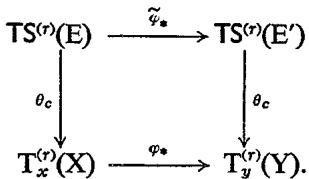
\includegraphics[keepaspectratio]{images/part001_e22e7577.jpg}}

该映射与 \(c\) 和 \(c'\) 的选取无关。若 \(t \in \mathrm{T}_{x}^{(r)}(\mathbf{X})\)，则称 \(\varphi_{*}(t)\) 为 \(t\) 经 \(\varphi\) 得到的像。我们有 \(\varphi_{*}(\varepsilon_{x}) = \varepsilon_{y}\)。若 \(k \leqslant r\)，则有

\[
\varphi_ {*} (\mathrm{T} _ {x} ^ {(k)} (\mathrm{X})) \subset \mathrm{T} _ {y} ^ {(k)} (\mathrm{Y}) \quad \text { and } \quad \varphi_ {*} (\mathrm{T} _ {x} ^ {(k) +} (\mathrm{X})) \subset \mathrm{T} _ {y} ^ {(k) +} (\mathrm{Y}).
\]

若 \(\varphi': X \to Y\) 是一个 \(C^r\) 类态射，且满足 \(\varphi'(x)=y\)，则 \(\varphi_* = \varphi_*'\) 当且仅当 \(j_x^r(\varphi) = j_x^r(\varphi')\)（参见 12.1）。

若 \(\varphi\) 在 \(x, \varphi_*\) 处是一个浸入（相应地，一个浸没），则它是单射（相应地，满射）；当 \(\dim_y Y < +\infty\) 时逆命题成立。

若 \(\varphi'\colon\mathbf{Y}\to\mathbf{Z}\) 是一个 \(\mathbf{C}^{r}\) 类流形态射，且 \(t\in\mathbf{T}_{x}^{(r)}(\mathbf{X})\)，则有 \((\varphi'\circ\varphi)_{*}(t)=\varphi_{*}^{\prime}(\varphi_{*}(t))\)。

设 F 是一个分离的多范数空间，f 是定义在 y 的一个邻域上、取值于 F 的 \(C^{r}\) 类函数。此时我们有

\[
\langle f, \varphi_ {*} (t) \rangle = \langle f \circ \varphi , t \rangle \quad \text {   for   all   } \quad t \in \mathrm{T} _ {x} ^ {(r)} (\mathrm{X}).\tag{1}
\]

对给定的 \(t\)，关系式 (1)（其中 \(f\) 与 \(F\) 为变量）刻画了 \(\varphi_{*}(t)\)；当 \(\dim_y Y < +\infty\) 时，可以只限于 \(F = K\) 的情形。

13.2.4. 假设 X 是 Banach 空间 E 的一个开子流形。用 \(\varphi_x\) 表示从 X 到 E 的映射 \(y \mapsto y - x\)；卡 \(c = (X, \varphi_x, E)\) 以 \(x\) 为中心。于是 \(\mathrm{T}_x^{(r)}(\mathbf{X})\) 与 \(\mathrm{TS}^{(r)}(\mathbf{E})\) 通过 \(\theta_c^{-1}\) 恒同。特别地，我们有 \(\mathrm{T}_x^{(\infty)}(\mathbf{X}) = \mathrm{TS}(\mathbf{E})\)。

设 F 是一个 Banach 空间，\(u: E \to F\) 是一个连续线性映射，且 \(x \in E\)，\(y \in F\) 满足 \(u(x) = y\)。如上所述，把 \(\mathrm{T}_{x}^{(\infty)}(E)\) 与 TS(E) 恒同，把 \(\mathrm{T}_{y}^{(\infty)}(F)\) 与 TS(F) 恒同。映射

\[
u _ {*} \colon \mathrm{TS(E)} \rightarrow \mathrm{TS(F)} \quad (\text { cf. } 13.2.3)
\]

与由 u 到张量代数的典范扩张所诱导的映射 TS(u) 一致。

13.2.5. 若 \(k \leqslant r\)，用 \(\mathrm{T}^{(k)}(\mathrm{X})\)（相应地，\(\mathrm{T}^{(k)+}(\mathrm{X})\)）表示诸 \(\mathrm{T}_a^{(k)}(\mathrm{X})\)（相应地，诸 \(\mathrm{T}_a^{(k)+}(\mathrm{X})\)，其中 \(a \in \mathrm{X}\)）的集合和。映射 \(t: \mathrm{X} \to \mathrm{T}^{(k)}(\mathrm{X})\) 若满足 \(t(a) \in \mathrm{T}_a^{(k)}(\mathrm{X})\)（对一切 \(a \in \mathrm{X}\)），则称为阶 \(\leqslant k\) 的点分布场。

假设 \(k\) 有限且 X 局部有限维。对每个 \(a \in X\)，双线性形式 \((j, t) \mapsto \langle j, t \rangle\)（参见 13.2.2）定义了一个同构 \(i_a\)，它把 \(\mathrm{T}_a^{(k)}(\mathrm{X})\) 映到 \(\mathrm{P}_a^k(\mathrm{X})^*\) 即 \(\mathrm{P}_a^k(\mathrm{X})\) 的对偶上。这些 \(i_a\) 定义了一个双射 \(i: \mathrm{T}^{(k)}(\mathrm{X}) \to \mathrm{P}^k(\mathrm{X})^*\)，其中 \(\mathrm{P}^k(\mathrm{X})^*\) 表示向量丛 \(\mathrm{P}^k(\mathrm{X})\) 的对偶；经由 \(i^{-1}\) 转移结构，我们给 \(\mathrm{T}^{(k)}(\mathrm{X})\) 装备一个以 X 为底、类为 \(\mathbf{C}^{r-k}\) 的向量丛结构。阶 \(\leqslant k\) 的点分布场称为 \(\mathbf{C}^s\) 类的（其中 \(s \leqslant r - k\)），如果它是 \(\mathbf{C}^s\) 类截面，即丛 \(\mathrm{T}^{(k)}(\mathrm{X})\) 的截面。

设 \(\varphi\colon\mathbf{X}\to\mathbf{Y}\) 是一个 \(\mathbf{C}^{r}\) 类流形态射，并假设 Y 与 X 一样是局部有限维的。那么 \(\varphi_{*}\colon\mathrm{T}^{(k)}(\mathrm{X})\to\mathrm{T}^{(k)}(\mathrm{Y})\) 是一个向量丛的 \(\varphi\)-态射，其类为 \(\mathbf{C}^{r-k}\)。

13.2.6. 设 \(k\) 是满足 \(0 \leqslant k \leqslant r\) 的整数。若 U 是有限维 Banach 空间 E 的一个开集，则依据 13.2.4，向量丛 \(\mathbf{T}^{(k)}(\mathbf{U})\) 与以 \(\mathbf{TS}^{(k)}(\mathbf{E})\) 为纤维的平凡丛恒同。

特别地，取 \(E = K^n\)，其中 \(n \geqslant 0\)，并设 \((e_1, \ldots, e_n)\) 为 \(E\) 的典范基。若 \(\alpha = (\alpha_1, \ldots, \alpha_n)\) 是 \(N^n\) 的一个元素，用 \(\Delta^\alpha\) 表示元素 \(\gamma_{\alpha_1}(e_1) \ldots \gamma_{\alpha_n}(e_n)\)（\(TS(E)\) 中的元素，所用的乘积是对称张量的对称积，参见 A, IV, § 5, no. 3）。\(^{(1)}\) 诸 \(\Delta^\alpha\)（其中 \(|\alpha| \leqslant k\)）构成 \(TS^{(k)}(E)\) 的一个基；若 \(a \in K^n\)，用 \(\Delta_a^\alpha\) 表示 \(T_a^{(k)}(E)\) 中相应的元素。设 F 是一个分离的多范数空间，f 是 \(C^r\) 类、定义在 \(a\) 的一个邻域内且取值于 F 的函数；若 \(\alpha \in N^n\)，则元素 \(\langle f, \Delta_a^\alpha \rangle\) 与 2.5.3、3.2.1 和 4.2.1 中定义的元素 \((\Delta^\alpha f)(a)\) 一致。

假设 X 局部有限维，并设 \(\xi = (\xi^1, \ldots, \xi^n)\) 是 X 在开集 U 上的一个坐标系。若 \(a \in \mathbf{U}\) 且 \(\alpha\) 是满足 \(|\alpha| \leqslant k\) 的多重指标，则用 \((\Delta_{\xi}^{\alpha})_a\) 表示点 \(a\) 处这样的点分布：它在 \(\xi\) 下的像是点分布 \(\Delta_{\xi(a)}^{\alpha}\)（在 \(\mathbf{K}^n\) 上）；分布场

\[
\Delta_ {\xi} ^ {\alpha}: a \mapsto (\Delta_ {\xi} ^ {\alpha}) _ {a} \quad (| \alpha | \leqslant k)
\]

构成向量丛 \(\mathbf{T}^{(k)}(\mathbf{X})\) 在 U 上的一个标架。若 \(f\colon \mathbf{U}\to \mathbf{F}\) 是 \(\mathbf{C}^r\) 类的，我们令 \(\langle f, (\Delta_{\xi}^{\alpha})_a\rangle = \Delta_{\xi}^{\alpha}f(a)\)，并用 \(\Delta_{\xi}^{\alpha}f\) 表示函数 \(a\mapsto \Delta_{\xi}^{\alpha}f(a)\)；它是 U 上的一个 \(\mathbf{C}^{r - k}\) 类函数。

\(^{1}\) 若 \(m = |\alpha|\)，且 \(\Sigma\) 是映射 \(\sigma\)（从 \(\{1, \ldots, m\}\) 到 \(\{1, \ldots, n\}\)、满足 \(\operatorname{Card}\sigma^{-1}(i)=\alpha_i\)）全体的集合，则有

\[
\Delta^ {\alpha} = \gamma_{\alpha_1}(e_1) \dots \gamma_{\alpha_n}(e_n) = \sum_{\sigma \in \Sigma} e_{\sigma(1)} \otimes \dots \otimes e_{\sigma(n)}, \quad \text { cf. A, IV, } \S 5, \text { no. } 4.
\]

\subsection{点分布与切空间}

在本节中，X 表示一个 C \(^{r}\) 类流形。

13.3.1. 设 \(x \in X\)，并设 \(k\) 是一个 \(\leqslant r\) 的整数。设 \(c = (U, \varphi, E)\) 是 \(X\) 的以 \(x\) 为中心的一个卡；13.2.1 中定义的同构 \(\theta_c \colon \mathsf{TS}^{(r)}(E) \to \mathsf{T}_x^{(r)}(X)\) 把 \(\mathsf{TS}^{(k)}(E)\) 映到 \(\mathsf{T}_x^{(k)}(X)\) 上，把 \(\mathsf{TS}^{(k-1)}(E)\) 映到 \(\mathsf{T}_x^{(k-1)}(X)\) 上；通过取限制和取商，它诱导出同构

\[
\theta_ {c, k} \colon \mathsf {T S} ^ {k} (\mathrm{E}) = \mathsf {T S} ^ {(k)} (\mathrm{E}) / \mathsf {T S} ^ {(k - 1)} (\mathrm{E}) \rightarrow \mathsf {T} _ {x} ^ {(k)} (\mathrm{X}) / \mathsf {T} _ {x} ^ {(k - 1)} (\mathrm{X}).
\]

另一方面，c 定义了一个同构，仍记作 \(\theta_{c}\)（参见 5.5.1），它把 E 映到切空间 \(T_{x}(X)\) 上。用 \(i_{k}\) 表示复合映射

\[
\mathrm{T} _ {x} ^ {(k)} (\mathrm{X}) / \mathrm{T} _ {x} ^ {(k - 1)} (\mathrm{X}) \xrightarrow {\theta_ {c , k} ^ {- 1}} \mathrm{TS} ^ {k} (\mathrm{E}) \xrightarrow {\mathrm{TS} ^ {k} (\theta_ {c})} \mathrm{TS} ^ {k} (\mathrm{T} _ {x} (\mathrm{X})).
\]

同构 \(i_k\) 与 \(c\) 的选取无关；当 \(k = 1\) 时，用它把 \(\mathrm{T}_x^{(1)+}(\mathrm{X}) = \mathrm{T}_x^{(1)}(\mathrm{X}) / \mathrm{T}_x^{(0)}(\mathrm{X})\) 与切空间 \(\mathrm{T}_x(\mathrm{X})\) 恒同。若 \(t \in \mathrm{T}_x^{(k)}(\mathrm{X})\)，可以把 \(i_k(t)\) 记为 \(i_k\) 作用于 \(t\) 模 \(\mathrm{T}_x^{(k-1)}(\mathrm{X})\) 的类而得的像。

令

\[
\operatorname{gr} _ {k} \mathrm{T} _ {x} ^ {(r)} (\mathrm{X}) = \mathrm{T} _ {x} ^ {(k)} (\mathrm{X}) / \mathrm{T} _ {x} ^ {(k - 1)} (\mathrm{X}) \quad \text { and } \quad \operatorname{gr} \mathrm{T} _ {x} ^ {(r)} (\mathrm{X}) = \bigoplus_ {0 \leqslant k \leqslant r} \operatorname{gr} _ {k} \mathrm{T} ^ {(r)} (\mathrm{X}).
\]

我们称 gr \(\mathbf{T}_{x}^{(r)}(\mathbf{X})\) 为与滤链 \((\mathbf{T}_{x}^{(k)}(\mathbf{X}))_{k\leq r}\)（\(\mathbf{T}_{x}^{(r)}(\mathbf{X})\) 的递增滤链）相伴的分次对象。诸 \(i_k\) 定义了一个分次向量空间的同构

\[
i \colon \operatorname{gr} \mathrm{T} _ {x} ^ {(r)} (\mathrm{X}) \rightarrow \mathrm{TS} ^ {(r)} (\mathrm{T} _ {x} (\mathrm{X})).
\]

若 \(r = \infty\) 或 \(\omega\)，则 \(i\) 是 gr \(T_x^{(r)}(X)\) 到 \(TS(T_x(X))\) 上的同构。当希望指明 \(x\)（或 X，或两者）时，就写 \(i_x\)（或 \(i_X\)，或 \(i_{X,x}\)）以代替 \(i\)。

13.3.2. 在上述假设之外，再假设 X 局部有限维。相对于 X 各点的诸同构 \(i_{k}\) 定义了一个向量丛同构

\[
i _ {k} \colon \mathrm{T} ^ {(k)} (\mathrm{X}) / \mathrm{T} ^ {(k - 1)} (\mathrm{X}) \rightarrow \mathrm{TS} ^ {k} (\mathrm{T} (\mathrm{X}))
\]

其中 TS \(^{k}\) (T(X)) 表示 C \(^{r-1}\) 类的、由有限维向量函子 TS \(^{k}\) 从 T(X) 得到的向量丛（参见 7.6.5）。当 \(k \geqslant 1\) 时，\(i_{k}\) 是一个 C \(^{r-k}\) 类同构；当 \(k = 0\) 时，它是平凡丛 \(\mathrm{K}_{\mathrm{X}}\) 的恒同映射。

13.3.3. 例。—— 在上述假设下，设 \(\xi = (\xi^{1}, \ldots, \xi^{n})\) 是 X 在 \(x\) 处的一个坐标系。用 \((\partial_{i,x})_{1 \leqslant i \leqslant n}\) 表示 \(\mathrm{T}_{x}(\mathrm{X})\) 的由 \(\xi\) 定义的基（参见 5.5.8），并用 \(((\Delta_{\xi}^{\infty})_{x})_{|\alpha| \leqslant k}\) 表示 13.2.6 中定义的 \(\mathrm{T}_{x}^{(k)}(\mathrm{X})\) 的基。我们有：

\[
\begin{array}{l l} i _ {k} ((\Delta_ {\xi} ^ {\alpha}) _ {x}) = 0 & \text {if} \quad | \alpha | <   k \\ i _ {k} ((\Delta_ {\xi} ^ {\alpha}) _ {x}) = \gamma_ {\alpha_ {1}} (\partial_ {1, x}) \dots \gamma_ {\alpha_ {n}} (\partial_ {n, x}) & \text {if} \quad | \alpha | = k. ^ {(1)} \end{array}
\]

\(^{1}\) 这里同样，诸 \(\gamma_{\alpha_{i}}(\partial_{i,x})\) 的乘积是 \(\mathrm{TS}(\mathrm{T}_{x}(\mathrm{X}))\) 中的对称积。

13.3.4. 假设 K 的特征为零，或者 X 局部有限维。设 k 是满足 \(0 \leqslant k \leqslant r\) 的整数，并设 \(x \in X\)；设 F 是一个 Banach 空间。根据 12.6.8，我们有正合序列

\[
0 \rightarrow \mathrm{P} _ {k} (\mathrm{T} _ {x} (\mathrm{X}); \mathrm{F}) \stackrel {{\iota}} {{\rightarrow}} \mathrm{P} _ {x} ^ {k} (\mathrm{F} _ {\mathrm{X}}) \stackrel {{\sigma}} {{\rightarrow}} \mathrm{P} _ {x} ^ {k - 1} (\mathrm{F} _ {\mathrm{X}}) \rightarrow 0,\tag{i}
\]

其中 \(\sigma = r^{k, k-1}\)。另一方面，根据 13.3.1，我们有正合序列

\[
0 \leftarrow \mathsf {T S} ^ {k} (\mathrm{T} _ {x} (\mathrm{X})) \stackrel {{i}} {{\leftarrow}} \mathrm{T} _ {x} ^ {(k)} (\mathrm{X}) \stackrel {{s}} {{\leftarrow}} \mathrm{T} _ {x} ^ {(k - 1)} (\mathrm{X}) \leftarrow 0,\tag{ii}
\]

其中 s 是 \(\mathrm{T}_{x}^{(k-1)}(\mathrm{X})\) 到 \(\mathrm{T}_{x}^{(k)}(\mathrm{X})\) 的包含映射，且 \(i=i_{k}\)。这些正合序列在 F 中“成对”。更确切地说，把它们写成如下形式：

\begin{enumerate}
\def\labelenumi{(\roman{enumi})}
\tightlist
\item
\end{enumerate}

\[
0 \rightarrow \mathrm{A} \xrightarrow {\iota} \mathrm{B} \xrightarrow {\sigma} \mathrm{C} \rightarrow 0\tag{ii}
\]

\[
0 \leftarrow A ^ {\prime} \stackrel {i} {\leftarrow} B ^ {\prime} \stackrel {s} {\leftarrow} C ^ {\prime} \leftarrow 0.
\]

若 \(a \in \mathbf{A}\) 且 \(a' \in \mathbf{A}'\)，F 中的元素 \(\langle a, a' \rangle\) 由 13.1.2 定义；若 \(b \in \mathbf{B}\) 且 \(b' \in \mathbf{B}'\)（相应地，若 \(c \in \mathbf{C}\) 且 \(c' \in \mathbf{C}'\)），F 中的元素 \(\langle b, b' \rangle\)（相应地，\(\langle c, c' \rangle\)）由 13.2.2 定义；于是有：

\[
\langle \iota a, b ^ {\prime} \rangle = \langle a, i b ^ {\prime} \rangle \quad \text { and } \quad \langle \sigma b, c ^ {\prime} \rangle = \langle b, s c ^ {\prime} \rangle \quad \text { if } \quad a \in \mathbf {A}, \quad b \in \mathbf {B}, \quad b ^ {\prime} \in \mathbf {B} ^ {\prime}, \quad c ^ {\prime} \in \mathbf {C} ^ {\prime}.
\]

13.3.5. 设 Y 是一个 \(C^{r}\) 类流形，\(\varphi: X \to Y\) 是一个 \(C^{r}\) 类态射，并设 \(x \in X\)，\(y \in Y\) 满足 \(y = \varphi(x)\)。13.2.3 中定义的映射 \(\varphi_{*}: T_{x}^{(r)}(X) \to T_{y}^{(r)}(Y)\) 与这些空间的滤链相容；通过转到相伴分次对象，它定义了一个线性映射

\[
\operatorname{gr} \left(\varphi_ {*}\right): \operatorname{gr} \mathrm{T} _ {x} ^ {(r)} (\mathrm{X}) \rightarrow \operatorname{gr} \mathrm{T} _ {y} ^ {(r)} (\mathrm{Y}).
\]

我们也用 \(\mathsf{TS}^{(r)}(\mathsf{T}_x(\varphi))\) 表示从 \(\mathsf{TS}^{(r)}(\mathsf{T}_x(\mathbf{X}))\) 到 \(\mathsf{TS}^{(r)}(\mathsf{T}_y(\mathbf{Y}))\) 的、由典范扩张 \(\mathsf{TS}(\mathsf{T}_x(\varphi))\)（\(\mathsf{T}_x(\varphi)\) 的典范扩张）诱导的映射。图表

\[
\begin{array}{c} \operatorname{gr} T _ {x} ^ {(r)} (X) \xrightarrow {\operatorname{gr} (\varphi_ {*})} \operatorname{gr} T _ {y} ^ {(r)} (Y) \\ \Biggl \downarrow i _ {\mathbf {X}, x} \\ \operatorname{TS} ^ {(r)} (T _ {x} (X)) \xrightarrow {\operatorname{TS} ^ {(r)} (T _ {x} (\varphi))} \operatorname{TS} ^ {(r)} (T _ {y} (Y)) \end{array}
\]

是交换的。

13.3.6. 假设 K 的特征为零。利用 A, IV, § 5, no. 8 中定义的同构 \(\varphi_{\mathbb{M}}: \mathsf{S}^k(\mathbf{M}) \to \mathsf{TS}^k(\mathbf{M})\)，可以在前述所有内容中把 \(\mathsf{TS}^k(\mathbf{T}_x(\mathbf{X}))\) 换成 \(k\) 次对称幂 \(\mathsf{S}^k(\mathbf{T}_x(\mathbf{X}))\)，即切空间 \(\mathbf{T}_x(\mathbf{X})\) 的对称幂。

\subsection{点分布的张量积}

13.4.1. 设 \(\mathbf{X}_1\) 与 \(\mathbf{X}_2\) 是两个 \(\mathbf{C}^r\) 类流形，设 \(x_1 \in \mathbf{X}_1\)，\(x_2 \in \mathbf{X}_2\)，以及 \(t_1 \in \mathrm{T}_{x_1}^{(k_1)}(\mathbf{X}_1)\)，\(t_2 \in \mathrm{T}_{x_2}^{(k_2)}(\mathbf{X}_2)\)，其中 \(k_1 + k_2 \leqslant r\)。令 \(\mathbf{X} = \mathbf{X}_1 \times \mathbf{X}_2\)，\(x = (x_1, x_2)\)，\(k = k_{1} + k_{2}\)。对 \(i = 1, 2\)，设 \(c_{i} = (U_{i}, \varphi_{i}, E_{i})\) 是 \(X_{i}\) 的以 \(x_{i}\) 为中心的卡，并用 \(\tilde{t}_{i}\) 表示 \(TS(E_{i})\) 中满足 \(\theta_{c_i}(\tilde{t}_{i}) = t_{i}\) 的元素（参见 13.2.1）。设 \(\sigma\) 是 \(TS(E_{1}) \otimes TS(E_{2})\) 到 \(TS(E_{1} \times E_{2})\) 上的典范同构（参见 A, IV, § 5, no. 5）。元素 \(\sigma(\tilde{t}_{1} \otimes \tilde{t}_{2})\) 是 \(\tilde{t}_{1}\) 与 \(\tilde{t}_{2}\)（视为 \(TS(E_{1} \times E_{2})\) 中的元素，借助典范单射 \(TS(E_{i}) \to TS(E_{1} \times E_{2})\)）的对称积；它属于 \(TS^{(k)}(E_{1} \times E_{2})\)。令 \(c = c_{1} \times c_{2}\)；它是 X 的以 \(x\) 为中心的卡。\(\theta_{c}\) 把 \(\sigma(\tilde{t}_{1} \otimes \tilde{t}_{2})\) 映为 \(T_{x}^{(k)}(X)\) 的一个元素，它与卡 \(c_{i}\) 的选取无关。把它称为 \(t_{1}\) 与 \(t_{2}\) 的直积或对称张量积（甚至简称张量积），并记作 \(t_{1} \times t_{2}\) 或 \(t_{1} \otimes t_{2}\)。

我们有 \(\varepsilon_{x_1} \otimes \varepsilon_{x_2} = \varepsilon_x\)。\(t_1 \otimes t_2\) 的常数项是 \(t_1\) 与 \(t_2\) 的常数项之积。

同构 \((y_{1}, y_{2}) \mapsto (y_{2}, y_{1})\)（从 \(\mathbf{X}_{1} \times \mathbf{X}_{2}\) 到 \(\mathbf{X}_{2} \times \mathbf{X}_{1}\) 上的同构）把 \(t_{1} \otimes t_{2}\) 变为 \(t_{2} \otimes t_{1}\)。

13.4.2（“结合性与函子性”）。设 \(X_{i}\)（i = 1, 2, 3）是 \(C^{r}\) 类流形，并设 \(x_{i} \in X_{i}\)，\(t_{i} \in \mathbf{T}_{x_{i}}^{(k_{i})}(\mathbf{X}_{i})\)，其中 \(k_{1} + k_{2} + k_{3} \leqslant r\)。我们有

\[
\left(t _ {1} \otimes t _ {2}\right) \otimes t _ {3} = t _ {1} \otimes \left(t _ {2} \otimes t _ {3}\right);
\]

把这个点分布记作 \(t_{1} \otimes t_{2} \otimes t_{3}\)。以同样方式定义任意有限的张量积。

设 \(\varphi_{1}\colon\mathbf{X}_{1}\to\mathbf{Y}_{1}\) 与 \(\varphi_{2}\colon\mathbf{X}_{2}\to\mathbf{Y}_{2}\) 是 \(\mathbf{C}^{r}\) 类流形态射，并设 \(t_{1}\in\mathbf{T}^{(k_{1})}(\mathbf{X}_{1})\)，\(t_{2}\in\mathbf{T}^{(k_{2})}(\mathbf{X}_{2})\)，其中 \(k_{1}+k_{2}\leqslant r\)。我们有

\[
(\varphi_ {1} \times \varphi_ {2}) _ {*} (t _ {1} \otimes t _ {2}) = \varphi_ {1 *} (t _ {1}) \otimes \varphi_ {2 *} (t _ {2}).
\]

13.4.3. 沿用 13.4.1 的记号，设 \(F_{1}\)、\(F_{2}\) 与 F 是分离的多范数空间，并设 \((u_{1}, u_{2}) \mapsto u_{1}.u_{2}\) 是从 \(F_{1} \times F_{2}\) 到 F 的一个连续双线性映射。设

\[
f _ {i} \colon \mathrm{X} _ {i} \rightarrow \mathrm{F} _ {i} \quad (i = 1, 2)
\]

是 \(\mathbf{C}^r\) 类映射，并用下式定义 \(f_1 \otimes f_2: \mathbf{X} \to \mathbf{F}\)：

\[
(f _ {1} \otimes f _ {2}) (y _ {1}, y _ {2}) = f _ {1} (y _ {1}). f _ {2} (y _ {2}).
\]

映射 \(f_{1} \otimes f_{2}\) 是 \(\mathbf{C}^{r}\) 类的，且我们有

\[
\langle f _ {1} \otimes f _ {2}, t _ {1} \otimes t _ {2} \rangle = \langle f _ {1}, t _ {1} \rangle . \langle f _ {2}, t _ {2} \rangle .
\]

13.4.4. 沿用 13.4.1 中的记号，设 \(f\) 是从 X 到分离的多范数空间 F 的一个 \(\mathbf{C}^{r}\) 类映射。若 \(y_{1} \in \mathbf{X}_{1}\)，用 \(f_{y_{1}}\) 表示映射 \(y_{2} \mapsto f(y_{1}, y_{2})\)（从 \(\mathbf{X}_{2}\) 到 F 的映射），并令 \(g(y_{1}) = \langle f_{y_{1}}, t_{2} \rangle\)。这样定义的函数 \(g: \mathbf{X}_{1} \to \mathbf{F}\) 是 \(\mathbf{C}^{r - k_{1}}\) 类的，且我们有

\[
\langle f, t _ {1} \otimes t _ {2} \rangle = \langle g, t _ {1} \rangle ,
\]

换言之

\[
\langle f, t _ {1} \otimes t _ {2} \rangle = \langle y _ {1} \mapsto \langle y _ {2} \mapsto f (y _ {1}, y _ {2}), t _ {2} \rangle , t _ {1} \rangle .
\]

同样我们有

\[
\langle f, t _ {1} \otimes t _ {2} \rangle = \langle y _ {2} \mapsto \langle y _ {1} \mapsto f (y _ {1}, y _ {2}), t _ {1} \rangle , t _ {2} \rangle .
\]

13.4.5. 沿用 13.4.1 中的记号，设

\[
\alpha_ {k _ {1}, k _ {2}} \colon \mathrm{T} _ {x _ {1}} ^ {(k _ {1})} (\mathrm{X} _ {1}) \otimes \mathrm{T} _ {x _ {2}} ^ {(k _ {2})} (\mathrm{X} _ {2}) \rightarrow \mathrm{T} _ {x} ^ {(k)} (\mathrm{X})
\]

为由双线性映射 \((t_{1}, t_{2}) \mapsto t_{1} \otimes t_{2}\) 定义的线性映射；该映射是单射；当 \(k_{1}\) 与 \(k_{2}\) 都是无穷时，它是双射。

若 \(n \leqslant r\)，用 \(\mathrm{T}_{x}^{(n)}(\mathrm{X}_{1}, \mathrm{X}_{2})\) 表示 \(\mathrm{T}_{x_{1}}^{(n)}(\mathrm{X}_{1}) \otimes \mathrm{T}_{x_{2}}^{(n)}(\mathrm{X}_{2})\) 中由诸子空间 \(\mathrm{T}_{x_{1}}^{(k_{1})}(\mathrm{X}_{1}) \otimes \mathrm{T}_{x_{2}}^{(k_{2})}(\mathrm{X}_{2})\)（\(k_{1} + k_{2} \leqslant n\)）生成的向量子空间。存在一个线性映射

\[
\alpha_ {n} \colon \mathrm{T} _ {x} ^ {(n)} (\mathrm{X} _ {1}, \mathrm{X} _ {2}) \rightarrow \mathrm{T} _ {x} ^ {(n)} (\mathrm{X})
\]

且是唯一的、延拓上述映射 \(\alpha_{k_1,k_2}\) 的线性映射；它是一个同构。在下文中，我们把 \(\mathrm{T}_x^{(n)}(\mathrm{X})\) 借助 \(\alpha_n^{-1}\) 与 \(\mathrm{T}_x^{(n)}(\mathrm{X}_1,\mathrm{X}_2)\)（\(\mathrm{T}_{x_1}^{(n)}(\mathrm{X}_1)\otimes \mathrm{T}_{x_2}^{(n)}(\mathrm{X}_2)\) 的向量子空间）恒同。

13.4.6. 我们保留 13.4.5 和 13.3.1 的记号。通过取商，\(\alpha_{k_1,k_2}\) 定义了一个线性映射

\[
\varepsilon_ {k _ {1}, k _ {2}} \colon \operatorname{gr} _ {k _ {1}} \mathrm{T} _ {x _ {1}} ^ {(r)} (\mathrm{X} _ {1}) \otimes \operatorname{gr} _ {k _ {2}} \mathrm{T} _ {x _ {2}} ^ {(r)} (\mathrm{X} _ {2}) \rightarrow \operatorname{gr} _ {k} \mathrm{T} _ {x} ^ {(r)} (\mathrm{X}).
\]

诸映射 \(\varepsilon_{k_1,k_2}\)（\(k_1 + k_2 \leqslant r\)）是一个零次分次线性映射的分量

\[
\varepsilon : \bigoplus_ {k _ {1} + k _ {2} \leqslant r} \left(\operatorname{gr} _ {k _ {1}} \mathrm{T} _ {x _ {1}} ^ {(r)} (\mathrm{X} _ {1}) \otimes \operatorname{gr} _ {k _ {2}} \mathrm{T} _ {x _ {2}} ^ {(r)} (\mathrm{X} _ {2})\right)\rightarrow \bigoplus_ {k \leqslant r} \operatorname{gr} _ {k} \mathrm{T} _ {x} ^ {(r)} (\mathrm{X})
\]

且该映射是一个同构。图表

\[
\begin{array}{l} \bigoplus_ {k _ {1} + k _ {2} \leqslant r} (\operatorname{gr} _ {k _ {1}} \mathrm{T} _ {x _ {1}} ^ {(r)} (\mathrm{X} _ {1}) \otimes \operatorname{gr} _ {k _ {2}} \mathrm{T} _ {x _ {2}} ^ {(r)} (\mathrm{X} _ {2})) \xrightarrow {\varepsilon} \operatorname{gr} \mathrm{T} _ {x} ^ {(r)} (\mathrm{X}) \\ \Biggl \downarrow i _ {1 2} \\ \bigoplus_ {k _ {1} + k _ {2} \leqslant r} (\mathrm{TS} ^ {k _ {1}} (\mathrm{T} _ {x _ {1}} (\mathrm{X} _ {1})) \otimes \mathrm{TS} ^ {k _ {2}} (\mathrm{T} _ {x _ {2}} (\mathrm{X} _ {2}))) \xrightarrow {\sigma} \bigoplus_ {k \leqslant r} \mathrm{TS} ^ {k} (\mathrm{T} _ {x _ {1}} (\mathrm{X} _ {1}) \times \mathrm{T} _ {x _ {2}} (\mathrm{X} _ {2})) \end{array}
\]

是交换的（在这个图中，\(i_{12}\) 表示由 \(i_{\mathbf{x}_1} \otimes i_{\mathbf{x}_2}\) 诱导的同态，而 \(\sigma\) 是 A, IV, § 5, no. 5 中定义的同构）。若 \(r\) 是无穷，这个图可以简单地写成：

\[
\begin{array}{l} \operatorname{gr} \mathrm{T} _ {x _ {1}} ^ {(\infty)} (\mathrm{X} _ {1}) \otimes \operatorname{gr} \mathrm{T} _ {x _ {2}} ^ {(\infty)} (\mathrm{X} _ {2}) \xrightarrow {\varepsilon} \operatorname{gr} \mathrm{T} _ {x} ^ {(\infty)} (\mathrm{X}) \\ \Biggl \downarrow_ {i _ {\mathbf {X} _ {1}} \otimes i _ {\mathbf {X} _ {2}}} \\ \operatorname{TS} (\mathrm{T} _ {x _ {1}} (\mathrm{X} _ {1})) \otimes \operatorname{TS} (\mathrm{T} _ {x _ {2}} (\mathrm{X} _ {2})) \xrightarrow {\sigma} \operatorname{TS} (\mathrm{T} _ {x} (\mathrm{X})). \end{array}
\]

\subsection{余积}

在本节中，X 表示一个 \(C^{r}\) 类流形，x 是 X 的一个点。

13.5.1. 设 \(k \leqslant r\)。若 \(\Delta\) 是对角映射 \(y \mapsto (y, y)\)，即从 X 到 \(X \times X\) 的对角映射，则 \(\Delta_*\) 把 \(\mathrm{T}_x^{(k)}(\mathrm{X})\) 映入 \(\mathrm{T}_{(x,x)}^{(k)}(\mathrm{X} \times \mathrm{X})\)，后者是 \(\mathrm{T}_{x}^{(k)}(\mathrm{X})\otimes\mathrm{T}_{x}^{(k)}(\mathrm{X})\) 的一个向量子空间（参见 13.4.5）。这样我们就得到一个线性映射，仍记作 \(\Delta_{*}\)（或 \(c\)）：

\[
\mathrm{T} _ {x} ^ {(k)} (\mathrm{X}) \rightarrow \mathrm{T} _ {x} ^ {(k)} (\mathrm{X}) \otimes \mathrm{T} _ {x} ^ {(k)} (\mathrm{X});
\]

我们把它称为附加于 \(\mathbf{T}_{x}^{(k)}(\mathbf{X})\) 的余积。装备了这个余积之后，\(\mathbf{T}_{x}^{(k)}(\mathbf{X})\) 是一个余结合且余交换的余代数（A, III, p. 144–145）；它以把每个点分布映为其常数项的线性形式（13.2.1）作为余单位。若 \(k' \leqslant k\)，则 \(\mathbf{T}_{x}^{(k')}(\mathbf{X})\) 到 \(\mathbf{T}_{x}^{(k)}(\mathbf{X})\) 的包含映射是余代数的态射。

若 \(c = (\mathrm{U},\varphi ,\mathrm{E})\) 是 \(\mathbf{X}\) 的以 \(x\) 为中心的卡，则同构

\[
\theta_ {c} \colon \mathrm{T} ^ {(k)} (\mathrm{E}) \rightarrow \mathrm{T} _ {x} ^ {(k)} (\mathrm{X})
\]

是一个余代数同构，其中 \(\mathrm{T}^{(k)}(\mathrm{E})\) 装备的是由 TS(E) 的余积诱导的余积（参见 A, IV, § 5, no. 7）。

若 \(\varphi: X \to Y\) 是一个 \(C^r\) 类流形态射，则从 \(T_x^{(k)}(X)\) 到 \(T_{\varphi(x)}^{(k)}(Y)\) 的、由 \(\varphi_*\) 诱导的映射是余代数的态射。

13.5.2. 设 \(F_{1}\)、\(F_{2}\) 与 F 是分离的多范数空间，并设 \((u_{1}, u_{2}) \mapsto u_{1}.u_{2}\) 是从 \(F_{1} \times F_{2}\) 到 F 的一个连续双线性映射。设 \(t \in \mathrm{T}_{x}^{(r)}(\mathrm{X})\)，并设它在余积下的像为 \(\boldsymbol{c}(t) = \sum_{j} u_{j} \otimes v_{j}\)，其中 \(u_{j},v_{j} \in \mathrm{T}_{x}^{(r)}(\mathrm{X})\)。设 \(f_{i}: X \to F_{i}\)（\(i=1,2\)）是 \(C^{r}\) 类映射。我们有

\[
\langle f _ {1}. f _ {2}, t \rangle = \sum_ {j} \langle f _ {1}, u _ {j} \rangle . \langle f _ {2}, v _ {j} \rangle ,
\]

按记号的滥用，我们把它写成：

\[
\langle f _ {1}. f _ {2}, t \rangle = \langle f _ {1} \otimes f _ {2}, c (t) \rangle .
\]

13.5.3. 设 \(t \in \mathbf{T}_x^{(k)}(\mathbf{X})\)，其中 \(k \leqslant r\)。

\begin{enumerate}
\def\labelenumi{\alph{enumi})}
\item
  要使 \(c(t)=t\otimes t\)，必须且只需 \(t\) 等于 0 或等于 \(\varepsilon_{x}\)。
\item
  要使 \(c(t)=t\otimes\varepsilon_{x}+\varepsilon_{x}\otimes t\)，必须且只需 \(t\) 是一个切向量，即 \(t\in\mathrm{T}_{x}^{(1)+}(X)\)。
\end{enumerate}

\subsection{有限支集分布}

13.6.1. 设 X 是一个 \(\mathbf{C}^r\) 类流形，并设 \(k \leqslant r\)。用 \(\mathcal{T}^{(k)}(\mathbf{X})\) 表示诸空间 \(\mathrm{T}_x^{(k)}(\mathbf{X})\)（\(x \in \mathbf{X}\)）的直和。\(\mathcal{T}^{(k)}(\mathbf{X})\) 的元素称为 \(\mathbf{X}\) 上阶 \(\leqslant k\) 的有限支集分布。若 \(f: \mathbf{X} \to \mathbf{F}\) 是 \(\mathbf{C}^r\) 类、取值于分离的多范数空间 \(\mathbf{F}\) 的函数，且 \(t = \sum_{x \in \mathbf{X}} t_x\)（其中 \(t_x \in \mathrm{T}_x^{(k)}(\mathbf{X})\) 对一切 \(x \in \mathbf{X}\) 成立）是一个有限支集分布，则我们令

\[
\langle f, t \rangle = \sum_ {x \in X} \langle f, t _ {x} \rangle .
\]

类似地，我们令 \(c(t) = \sum_{x \in X} c(t_x)\)，这给 \(\mathcal{T}^{(k)}(X)\) 装备了一个以 \(t \mapsto \langle 1, t \rangle\) 为余单位的余结合、余交换余代数结构。包含映射 \(\mathcal{T}^{(k')}(X) \to \mathcal{T}^{(k)}(X)\)（其中 \(k' \leqslant k\)）是余代数的态射。

若 \(\varphi: X \to Y\) 是一个 \(C^r\) 类流形态射，则诸映射 \(\mathrm{T}_x^{(k)}(\varphi): \mathrm{T}_x^{(k)}(X) \to \mathrm{T}_{\varphi(x)}^{(k)}(Y)\)（其中 \(x\) 取遍 \(X\)）定义了一个线性映射 \(\varphi_*\)，它把 \(\mathcal{T}^{(k)}(X)\) 映到 \(\mathcal{T}^{(k)}(Y)\)，且是余代数的态射。

若 \(X_{1}\) 与 \(X_{2}\) 是两个 \(C^{r}\) 类流形，则诸映射 \(\alpha_{k}^{-1}\)（参见 13.4.5）定义了一个线性映射

\[
\mathcal {T} ^ {(k)} \left(\mathrm{X} _ {1} \times \mathrm{X} _ {2}\right)\rightarrow \mathcal {T} ^ {(k)} \left(\mathrm{X} _ {1}\right) \otimes \mathcal {T} ^ {(k)} \left(\mathrm{X} _ {2}\right)
\]

它是单射；它是余代数的态射。若 \(k = \infty\) 或 \(\omega\)，它是余代数的同构。

13.6.2. 设 X 是一个 \(C^{r}\) 类流形，V 是一个有限维 K-向量空间。\(\mathcal{T}^{(r)}(\mathrm{X})\otimes\mathrm{V}\) 的元素称为 X 上取值于 V 的有限支集分布。当 K = R、V = C 时，这样的分布也称为 X 上的复有限支集分布。前面各条的定义和结论通过线性性立即推广到取值于 V 的分布。

\subsection{结构弱化}

我们假设 \(\mathbf{K} = \mathbf{R}\)。设 \(r' \in \mathrm{N}_{\mathbb{K}}\) 满足 \(r' \leqslant r\)。设 X 是一个 \(\mathbf{C}^{r}\) 类流形，\(\mathbf{X}'\) 是通过结构弱化（5.13.1）得到的 \(\mathbf{C}^{r'}\) 类流形。设 \(x \in \mathbf{X}\)，并设 \(t \in \mathrm{T}_x^{(k)}(\mathbf{X})\)，其中 \(k \leqslant r'\)。取 X 的一个卡 \(c = (\mathrm{U}, \varphi, \mathrm{E})\)，其中心为 \(x\)，并用 \(\tilde{t}\) 表示 \(\mathrm{TS}^{(k)}(\mathrm{E})\) 中满足 \(\theta_c(\tilde{t}) = t\) 的元素。由于 \(c\) 也是 \(\mathbf{X}'\) 的以 \(x\) 为中心的卡，元素 \(t' = \theta_c(\tilde{t})\)（\(\mathrm{T}_x^{(k)}(\mathrm{X}')\) 中的元素）有定义；它与 \(c\) 的选取无关。映射 \(t \mapsto t'\) 是 \(\mathrm{T}_x^{(k)}(\mathbf{X})\) 到 \(\mathrm{T}_x^{(k)}(\mathbf{X}')\) 上的一个双射，借助它把这两个空间恒同。这样得到的恒同与前面各条中的运算 \(\langle f, t \rangle\)、\(\varphi_*(t)\)、\(t_1 \otimes t_2\)、\(c(t)\)、\ldots{} 相容。

\section{微分算子}

在本段中，X 表示一个局部有限维的 \(C^{r}\) 类流形，其中 \(r \in N_{K}\)；设 E 与 F 是两个以 X 为底的 \(C^{r}\) 类有限秩向量丛。

所考虑的所有流形和向量丛都假设是局部有限维的。

\subsection{微分算子}

14.1.1. 设 \(k\) 是满足 \(0 \leqslant k \leqslant r\) 的整数，并设 \(\mathbf{P}^k(\mathbf{E})\) 是 E 的 \(k\) 阶截面射流丛（12.6.1）。令

\[
\mathbf {D} ^ {k} (\mathbf {E}, \mathbf {F}) = \mathscr {L} (\mathbf {P} ^ {k} (\mathbf {E}); \mathbf {F}).
\]

它是一个以 X 为底、\(C^{r-k}\) 类的向量丛。这个丛在 X 的开集 U 上的截面等同于一个映射

\[
\mathbf {D}: \mathrm{P} ^ {k} (\mathrm{E}) | \mathrm{U} \rightarrow \mathrm{F} | \mathrm{U}
\]

它与到 U 上的投影交换，且在每个纤维上是线性的；这样的截面称为 U 上的 E \(\to\) F 型、阶 \(\leqslant k\) 的微分算子。设 \(h \in N_{K} \cup \{0\}\)，其中 \(0 \leqslant h \leqslant r-k\)。用 \(\mathcal{D}_{\mathrm{U}}^{k,h}(\mathrm{E}, \mathrm{F})\) 表示 U 上的 E \(\to\) F 型、阶 \(\leqslant k\) 且为 \(C^{h}\) 类（作为 \(\mathrm{D}^{k}(\mathrm{E}, \mathrm{F})\) 的截面，或作为 \(\mathrm{P}^{k}(\mathrm{E})|\mathrm{U}\) 到 \(\mathrm{F}|\mathrm{U}\) 的态射，二者是一回事）的微分算子全体组成的集合。若 \(\mathrm{M} = \mathrm{D}^{k}(\mathrm{E}, \mathrm{F})\)，则有 \(\mathcal{D}_{\mathrm{U}}^{k,h}(\mathrm{E}, \mathrm{F}) = \mathcal{S}_{\mathrm{M}}^{h}(\mathrm{U})\)；它是 \(\mathcal{C}^{h}(\mathrm{U})\) 上的模（参见 7.4.1）。

若 \(0 \leqslant k' \leqslant k\)，则态射 \(r^{k, k'}: \mathrm{P}^{k}(\mathrm{E}) \to \mathrm{P}^{k'}(\mathrm{E})\)（参见 12.6.6）定义了从 \(\mathrm{D}^{k'}(\mathrm{E}, \mathrm{F})\) 到 \(\mathrm{D}^{k}(\mathrm{E}, \mathrm{F})\) 的一个单射；从而每个阶 \(\leqslant k'\) 的微分算子都等同于一个阶 \(\leqslant k\) 的微分算子。一个阶 \(\leqslant k\) 但非阶 \(\leqslant k - 1\) 的微分算子有时称为 \(k\) 阶微分算子。若 \(h \in \mathbf{N}_{\mathbb{K}} \cup \{0\}\) 且 \(h \leqslant r - k\)，且 U 是 X 的开子集，则有：

\[
0 \subset \mathcal {D} _ {\mathrm{U}} ^ {0, h} (\mathrm{E}, \mathrm{F}) \subset \mathcal {D} _ {\mathrm{U}} ^ {1, h} (\mathrm{E}, \mathrm{F}) \subset \dots \subset \mathcal {D} _ {\mathrm{U}} ^ {k, h} (\mathrm{E}, \mathrm{F}).
\]

若 \(r=\infty\) 或 \(\omega\)，用 \(\mathcal{D}_{\mathrm{U}}^{\infty,h}(\mathrm{E},\mathrm{F})\) 表示诸 \(\mathcal{D}_{\mathrm{U}}^{k,h}(\mathrm{E},\mathrm{F})\)（\(k\geqslant0\)）的并；这个并的元素称为 U 上的有界阶微分算子（E \(\rightarrow\) F 型、C \(^{h}\) 类），有时也简称 U 上的微分算子。

14.1.2（“零阶算子”）。我们有 \(\mathbf{P}^0 (\mathbf{E}) = \mathbf{E}\)（12.5.1）以及 \(\mathrm{D}^0 (\mathrm{E},\mathrm{F}) = \mathcal{L}(\mathrm{E};\mathrm{F})\)。若 U 是 X 中的开集，且 \(h\in \mathbf{N}_{\mathbb{K}}\cup \{0\}\)、\(h\leqslant r\)，则 \(\mathcal{D}_{\mathbf{U}}^{0,h}(\mathbf{E},\mathbf{F})\) 的元素是 \(\mathbf{C}^h\) 类的、从 E\textbar U 到 F\textbar U 的态射。

14.1.3（“结构弱化”）。假设 K = R，并设 \(r' \in N_{R}\) 满足 \(r' \leqslant r\)。设 X'、E' 与 F' 分别是由 X、E 与 F 通过弱化结构得到的 \(C^{r'}\) 类流形和向量丛。设 k 是满足 \(0 \leqslant k \leqslant r'\) 的整数。那么 \(P^{k}(E')\) 是一个 \(C^{r'-k}\) 类丛，由 \(P^{k}(E)\) 通过弱化结构得到，对 \(D^{k}(E', F')\) 也有类似的结果。特别地，若 U 是 X 中的开集，且 \(0 \leqslant h \leqslant r - k'\)，则有 \(\mathcal{D}_{\mathrm{U}}^{k,h}(E', F') = \mathcal{D}_{\mathrm{U}}^{k,h}(E, F)\)。

14.1.4. 设 D 是 X 上的一个 E \(\to\) F 型、阶 \(\leqslant k\)（其中 \(0 \leqslant k \leqslant r\)）的微分算子。设 U 是 X 的开子集，s 是 E 在 U 上的一个 \(\mathbf{C}^{m}\) 类截面，其中 \(m \in N _{K} \cup \{0\}\) 且 \(k \leqslant m \leqslant r\)。那么 \(j^{k}(s)\) 是一个 \(\mathbf{C}^{m-k}\) 类截面，即 \(P^{k}(E)\) 在 U 上的截面（12.6.1）；它在 D 下的像记作 \(D_{U}(s)\) 或 D(s)。它是 F 在 U 上的一个截面。假设 D 是 \(\mathbf{C}^{h}\) 类的，其中 \(h=m-k\)。那么 \(D_{U}(s)\) 是 \(\mathbf{C}^{h}\) 类的，且诸映射

\[
\mathrm{D} _ {\mathrm{U}} \colon \mathcal {S} _ {\mathrm{E}} ^ {m} (\mathrm{U}) \rightarrow \mathcal {S} _ {\mathrm{F}} ^ {h} (\mathrm{U})
\]

具有下列性质：

\begin{enumerate}
\def\labelenumi{(\arabic{enumi})}
\item
  \(D_{U}\) 是 K-线性的。
\item
  对每个 \(s \in \mathcal{S}_{\mathbb{E}}^{m}(\mathrm{U})\) 及每个 \(\mathrm{V}\)（\(\mathrm{U}\) 的开集），有 \(\mathrm{D}_{\mathrm{V}}(s|\mathrm{V}) = \mathrm{D}_{\mathrm{U}}(s)|\mathrm{V}\)。
\item
  对每个 \(s \in \mathcal{S}_{\mathbb{E}}^{m}(\mathrm{U})\) 及每个 \(x \in \mathrm{U}\)（满足 \(j_{x}^{k}(s) = 0\)），有 \(D_{\mathrm{U}}(s)(x) = 0\)。
\end{enumerate}

(3') 对 U 内每个坐标系 \(\xi = (\xi^1, \ldots, \xi^n)\) 以及 E 在 U 上的任意标架 \(s = (s_1, \ldots, s_d)\)（7.4.4），存在 F 在 U 上的截面 \(n_{i,\alpha}(1 \leqslant i \leqslant d, \alpha \in \mathbf{N}^n, |\alpha| \leqslant k)\)（\(C^h\) 类的截面），使得对每个族 \((f_i)_{1 \leqslant i \leqslant d}\)（\(\mathcal{C}^m(U)\) 中元素的族），有

\[
\mathrm{D} _ {\mathrm{U}} \left(\sum_ {1 \leqslant i \leqslant d} f _ {i}. s _ {i}\right) = \sum_ {1 \leqslant i \leqslant d, | \alpha | \leqslant k} \Delta_ {\xi} ^ {\alpha} (f _ {i}). n _ {i, \alpha},
\]

\begin{enumerate}
\def\labelenumi{(\arabic{enumi})}
\setcounter{enumi}{3}
\tightlist
\item
  对任意函数 \(f \in \mathcal{C}^m(\mathrm{U})\) 及任意映射 \(\theta\)（从 \(\mathcal{S}_{\mathrm{U}}^{m}(\mathrm{E})\) 到 \(\mathcal{S}_{\mathrm{U}}^{h}(\mathrm{F})\)），用 \(\operatorname{ad}(f)\theta\) 表示映射
\end{enumerate}

\[
s \mapsto f. \theta (s) - \theta (f. s)
\]

（从 \(\mathcal{S}_{\mathrm{U}}^{m}(\mathrm{E})\) 到 \(\mathcal{S}_{\mathrm{U}}^{h}(\mathrm{F})\)）。那么，对每个函数 \(f \in \mathcal{C}^{m}(\mathrm{U})\)，存在一个微分算子 \(\mathbf{L}\)（\(\mathbf{U}\) 上的算子），它是 \(\mathrm{E} \to \mathrm{F}\) 型、阶 \(\leqslant k - 1\) 且 \(\mathbf{C}^{h}\) 类的，使得

\[
(\operatorname{ad} (f) \mathrm{D} _ {\mathrm{U}}) (s) = \mathrm{L} _{\mathrm{U}}(s) \quad \text { for all } s \in \mathscr{S}_{\mathrm{E}}^{m}(\mathrm{U}).
\]

\begin{enumerate}
\def\labelenumi{(\arabic{enumi})}
\setcounter{enumi}{4}
\tightlist
\item
  我们有
\end{enumerate}

\[
\operatorname{ad} (f _ {0}) \dots \operatorname{ad} (f _ {k}) \mathrm{D} _ {\mathrm{U}} = 0 \quad \text { for all } f _ {0}, \dots , f _ {k} \text { in } \mathscr {C} ^ {m} (\mathrm{U}).
\]

若令 I = \{0, . . ., k\}，并对 I 的每个子集 H 令 \(f_{H} = \prod_{i \in H} f_i\)，则前面的关系式等价于：

\[
\sum_ {\mathrm{H} \in \mathrm{I}} (- 1) ^ {\operatorname{Card} (\mathrm{H})} f _ {\mathrm{H}}. \mathrm{D} _ {\mathrm{U}} (f _ {\mathrm{I-H}}. s) = 0
\]

其中 \(f_{0},\ldots,f_{k}\) 取遍 \(\mathcal{C}^{m}(\mathrm{U})\)，\(s\) 取遍 \(\mathcal{S}_{\mathbf{E}}^{m}(\mathrm{U})\)。

14.1.5（“微分算子的刻画”）。设 \(k, m\) 与 \(h = m - k\) 如 14.1.4 所述。对 X 的每个开集 U，设 \(\mathbf{D}_{\mathbf{U}}\) 是从 \(\mathcal{S}_{\mathbf{E}}^{m}(\mathbf{U})\) 到 \(\mathcal{S}_{\mathbf{F}}^{h}(\mathbf{U})\) 的一个映射。假设对 X 的每个开子集 U，14.1.4 的条件 1、2、3（相应地，1、2、3'）都满足。那么存在 \(\mathcal{D}_{\mathbf{X}}^{k,h}(\mathbf{E},\mathbf{F})\) 中唯一的元素 D，使得诸 \(\mathbf{D}_{\mathbf{U}}\) 是相应的映射。\(^{(1)}\) 在下文中，我们把 D 与诸 \(\mathbf{D}_{\mathbf{U}}\) 组成的族恒同。

当 \(m = \infty\) 或 \(\omega\) 时，有 \(h = m\)，并且可以把条件 (3) 与 (3') 换成条件 (4) 或 (5) 之一。

14.1.6（“标量算子”）。假设 E 与 F 都等于平凡丛 \(K_{X}\)。这时 \(E \rightarrow F\) 型的微分算子称为标量微分算子，或简称微分算子；若它是阶 \(\leqslant k\) 的，则它是丛 \(\mathcal{L}(\mathrm{P}^{k}(\mathrm{X}); \mathrm{K}_{\mathrm{X}}) = \mathrm{P}^{k}(\mathrm{X})^{*}\)（丛 \(\mathrm{P}^{k}(\mathrm{X})\) 的对偶）的截面；利用同构

\[
i ^ {- 1} \colon \mathrm{P} ^ {k} (\mathrm{X}) ^ {*} \rightarrow \mathrm{T} ^ {(k)} (\mathrm{X}) \quad (\text { cf. } 13.2.5),
\]

可知阶 \(\leqslant k\) 的标量微分算子等同于向量丛 \(\mathbf{T}^{(k)}(\mathbf{X})\) 的截面，即阶 \(\leqslant k\) 的点分布场。

特别地，取 X 为 \(K^{n}\) 的一个开集，其中 n 是一个 \(\geqslant0\) 的整数。点分布场

\[
\Delta^ {\alpha} \colon x \mapsto \Delta_ {x} ^ {\alpha} \quad (\text { cf. } 1 3. 2. 6)
\]

都是 \(\mathbf{C}^{\omega}\) 类的标量微分算子。对每个 \(h\in\mathbf{N}_{\mathbf{K}}\)，诸 \(\Delta^{\alpha}\)（\((|\alpha|\leqslant k)\)）构成 \(\mathcal{C}^{h}(\mathbf{X})\)-模 \(\mathcal{D}_{\mathbf{X}}^{k,h}(\mathbf{K}_{\mathbf{X}},\mathbf{K}_{\mathbf{X}})\) 的一个基。

14.1.7（“实流形上的复微分算子”）。假设 K = R，且向量丛 E 与 F 都装备了复结构（8.8.1）；设 k 是满足 \(0 \leqslant k \leqslant r\) 的整数。这时丛 \(\mathrm{P}^{k}(\mathrm{E})\) 装备有一个复结构（12.6.3）；丛 \(\mathcal{L}_{\mathbf{C}}(\mathrm{P}^{k}(\mathrm{E}); \mathrm{F})\)（7.8.5，由 \(\mathrm{P}^{k}(\mathrm{E})\) 到 F 的复线性映射组成的丛）是 \(\mathcal{L}(\mathrm{P}^{k}(\mathrm{E}); \mathrm{F}) = \mathrm{D}^{k}(\mathrm{E}, \mathrm{F})\) 的一个向量子丛；我们把它记作 \(\mathrm{D}_{\mathbf{C}}^{k}(\mathrm{E}, \mathrm{F})\)。\(\mathrm{D}_{\mathbf{C}}^{k}(\mathrm{E}, \mathrm{F})\) 的截面称为 \(E \to F\) 型、阶 \(\leqslant k\) 的复微分算子。若 \(h \in N_{K}\) 且 \(h \leqslant r - k\)，且 U 是 X 的开集，我们类似地用 \(\mathcal{D}_{\mathbf{U}}^{k,h}(\mathrm{E}, \mathrm{F})_{\mathbf{C}}\) 表示 \(C^{h}\) 类截面（\(\mathrm{D}_{\mathbf{C}}^{k}(\mathrm{E}, \mathrm{F})\) 在 U 上的截面）所成的空间；它是一个 C-向量空间。本段的其他定义和结论类似地推广到复微分算子；其表述留给读者。

14.1.8（“复合”）。设 G 是一个以 X 为底的 \(C^{r}\) 类向量丛。设 \(k'\) 与 \(k''\) 是正整数，其和 \(k \leqslant r\)，并设 \(D'\)（相应地，\(D''\)）是 X 上的一个 \(E \to F\) 型（相应地，\(F \to G\) 型）、阶 \(\leqslant k'\)（相应地，\(\leqslant k''\)）的微分算子。假设 \(D': P^{k'}(E) \to F\) 是 \(C^{h'}\) 类的，其中 \(h' \in N_{K} \cup \{0\}\) 且 \(k'' \leqslant h' \leqslant r - k'\)；映射

\[
\mathbf {D} _ {*} ^ {\prime} = \mathbf {P} ^ {k ^ {\prime \prime}} (\mathbf {D} ^ {\prime}) \colon \mathbf {P} ^ {k ^ {\prime \prime}} (\mathbf {P} ^ {k ^ {\prime}} (\mathbf {E})) \rightarrow \mathbf {P} ^ {k ^ {\prime \prime}} (\mathbf {F})
\]

该映射是 \(\mathbf{C}^{h'-k''}\) 类的（12.6.3）。设 \(\beta\) 是从 \(\mathbf{P}^{k}(\mathbf{E})\) 到 \(\mathbf{P}^{k''}(\mathbf{P}^{k'}(\mathbf{E}))\) 的典范同态（参见 12.6.5）。把映射

\[
\mathrm{P} ^ {k} (\mathrm{E}) \xrightarrow {\beta} \mathrm{P} ^ {k ^ {\prime \prime}} (\mathrm{P} ^ {k ^ {\prime}} (\mathrm{E})) \xrightarrow {\mathrm{D} _ {*} ^ {\prime}} \mathrm{P} ^ {k ^ {\prime \prime}} (\mathrm{F}) \xrightarrow {\mathrm{D} ^ {\prime \prime}} \mathrm{G},
\]

复合起来，就得到一个 E → G 型、阶 ≤ k 的微分算子。这个算子称为 D'' 与 D' 的复合；记作 D'' ∘ D'。

\(^{1}\) 此外，只需条件 (3′) 对一个坐标系族 \((\xi_{\lambda})\) 和一个定义域覆盖 X 的标架族 \((s_{\lambda})\) 满足即可。

若 U 是 X 的开子集，且 \(s \in \mathcal{S}_{\mathrm{E}}^{k}(\mathrm{U})\)，则有

\[
(\mathbf {D} ^ {\prime \prime} \circ \mathbf {D} ^ {\prime}) (s) = \mathbf {D} ^ {\prime \prime} (\mathbf {D} ^ {\prime} (s))
\]

（其中两边都是 G 在 U 上的截面）；这印证了所采用的术语和记号。

现在假设 \(\mathbf{D}^{\prime \prime}\) 是 \(\mathbf{C}^{h^{\prime \prime}}\) 类的，其中 \(h^{\prime \prime} \in \mathrm{N}_{\mathbb{K}} \cup \{0\}\) 且 \(h^{\prime \prime} \leqslant r-k^{\prime\prime}\)。那么 \(\mathbf{D}^{\prime \prime} \circ \mathbf{D}^{\prime}\) 是 \(\mathbf{C}^{h}\) 类的，其中 \(h=\inf(h'-k'',h'')\)。

假设 E = F = G，且 \(k' \leqslant h''\)，此时 \(D' \circ D''\) 有定义。那么 \(D' \circ D'' - D'' \circ D'\) 是一个 \(E \to E\) 型、阶 \(\leqslant k - 1\) 的微分算子；我们把它记作 \([D', D'']\)。

14.1.9（“结合性”）。沿用 14.1.8 的记号与假设，设 H 是一个 \(\mathbf{C}^r\) 类、以 X 为底的向量丛，并设 \(\mathbf{D}''\) 是 X 上的一个 \(\mathbf{G} \to \mathbf{H}\) 型、阶 \(\leqslant k^{m}\) 的微分算子，其中 \(k' + k'' + k'' \leqslant r\)。我们假设 \(\mathbf{D}'\) 是 \(\mathbf{C}^{h'}\) 类的，其中 \(h' \in \mathrm{N}_{\kappa} \cup \{0\}\) 且 \(k'' + k'' \leqslant h' \leqslant r - k'\)；并假设 \(\mathbf{D}''\) 是 \(\mathbf{C}^{h''}\) 类的，其中 \(h'' \in \mathrm{N}_{\kappa} \cup \{0\}\) 且 \(k'' \leqslant h'' \leqslant r - k''\)。那么复合

\[
\mathbf {D} ^ {\prime \prime \prime} \circ (\mathbf {D} ^ {\prime \prime} \circ \mathbf {D} ^ {\prime}) \quad \text { and } \quad (\mathbf {D} ^ {\prime \prime \prime} \circ \mathbf {D} ^ {\prime \prime}) \circ \mathbf {D} ^ {\prime}
\]

都有定义并且相等。

14.1.10. 例子

\begin{enumerate}
\def\labelenumi{\alph{enumi})}
\tightlist
\item
  设 U 是 X 的开子集，\(D \in \mathcal{D}_{\mathrm{U}}^{k,h}(\mathrm{E}, \mathrm{F})\)，其中 \(h \in N_{K} \cup \{0\}\) 且 \(h \leqslant r-k\)，并设 \(f \in \mathcal{C}^{h+k}(\mathrm{U})\)（相应地，\(f \in \mathcal{C}^{h}(\mathrm{U})\)）。E（相应地，F）中乘以 f 的运算是 U 上的一个阶 \(\leqslant0\)、E \(\to\) E 型（相应地，F \(\to\) F 型）的微分算子（参见 14.1.2）。复合 \(D\circ f\) 与 \(f\circ D\) 有定义且属于 \(\mathcal{D}_{\mathrm{U}}^{k,h}(\mathrm{E},\mathrm{F})\)；我们令
\end{enumerate}

\[
\operatorname{ad} (f) \mathrm{D} = f \circ \mathrm{D} - \mathrm{D} \circ f \in \mathcal {D} _ {\mathrm{U}} ^ {k - 1, h} (\mathrm{E}, \mathrm{F}),
\]

（参见 14.1.4, (4)）。这样就给 \(\mathcal{D}_{\mathrm{U}}^{k,h}(\mathrm{E},\mathrm{F})\) 装备了一个右 \(\mathcal{C}^{h+k}(\mathrm{U})\)-模（相应地，左 \(\mathcal{C}^h (\mathrm{U})\)-模）结构。左模结构与 14.1.1 中的一致。

\begin{enumerate}
\def\labelenumi{\alph{enumi})}
\setcounter{enumi}{1}
\item
  假设 \(r = \infty\) 或 \(r = \omega\)。\(E \to E\) 型、\(C^r\) 类的微分算子构成一个含幺元素的结合 K-代数。
\item
  取 X 为 \(K^{n}\) 的一个开子集。标量微分算子 \(\Delta^{\alpha}\)（14.1.6）满足公式
\end{enumerate}

\[
\Delta^ {\alpha} \circ \Delta^ {\beta} = ((\alpha , \beta)) \Delta^ {\alpha + \beta}.
\]

它们彼此交换。用 \(D_{i}\) 表示算子 \(\Delta^{\varepsilon_{i}}\)（“第 i 个偏导数”）。若 K 的特征为 0，我们有

\[
\Delta^ {\alpha} = \frac {1}{\alpha !} D _ {1} ^ {\alpha_{1}} \dots D _ {n} ^ {\alpha_{n}}.
\]

若 K 的特征为 \(p \neq 0\)，则有 \(\mathbf{D}_{i}^{p} = 0\)（对一切 \(i\)）。

14.1.11（“多微分算子”）。设 \(E_{1}, \ldots, E_{n}\) 是以 X 为底的 \(C^{r}\) 类向量丛，并设 \(k, k_{1}, \ldots, k_{n}\) 是属于 \([0, r]\) 的整数。令

\[
\mathrm{L} (k _ {1}, \dots , k _ {n}) = \mathscr {L} (\mathrm{P} ^ {k _ {1}} (\mathrm{E} _ {1}) \otimes \dots \otimes \mathrm{P} ^ {k _ {n}} (\mathrm{E} _ {n}); \mathrm{F}).
\]

若 \(k_i \leqslant k\)（对一切 \(i\)），则投影 \(r^k, k_i: \mathrm{P}^k(\mathrm{E}_i) \to \mathrm{P}^{k_i}(\mathrm{E}_i)\) 使我们能把丛 \(\mathrm{L}(k_1, \ldots, k_n)\) 等同于丛 \(\mathrm{L}(k) = \mathrm{L}(k, \ldots, k)\) 的一个子丛。存在最小子丛 \(\mathrm{M}(k)\)（\(\mathrm{L}(k)\) 的子丛），它包含所有子丛 \(\mathrm{L}(k_1, \ldots, k_n)\)（\(k_1 + \cdots + k_n = k\)）。截面 \(\mathrm{H}\)（\(\mathrm{M}(k)\) 的截面）称为 \((\mathrm{E}_1, \ldots, \mathrm{E}_n) \to \mathrm{F}\) 型、阶 \(\leqslant k\) 的 n-微分算子（或多微分算子）。若 \(s_i\)（\(1 \leqslant i \leqslant n\)）是 \(\mathbf{C}^m (m \in \mathbb{N}_{\mathbb{K}}, m \geqslant k)\) 类截面（\(\mathbf{E}_i\) 在 X 的开集 U 上的截面），则把 \(\mathrm{H}_{\mathrm{U}}(s_1, \ldots, s_n) = \mathrm{H}(s_1, \ldots, s_n)\) 定义为下述丛的截面 \(j^k(s_1) \otimes \cdots \otimes j^k(s_n)\) 在 H 下的像：

\[
\mathbf {P} ^ {k} (\mathrm{E} _ {1}) \otimes \dots \otimes \mathbf {P} ^ {k} (\mathrm{E} _ {n}).
\]

它是 F\textbar U 的一个截面。若 H 是 \(\mathbf{C}^h\) 类的，则该截面是 \(\mathbf{C}^p\) 类的，其中 \(p = \inf(m - k, h)\)。

当 \(E_{1}, \ldots, E_{n}\) 与 F 都等于 \(K_{x}\) 时，称 H 为标量 n-微分算子（或标量多微分算子）。

例。—— 设 J 是一个有限集，X 是 K \(^{J}\) 的一个开子集。设 H 是 X 上的一个阶 \(\leqslant k\) 的标量 n-微分算子。存在唯一的标量函数族

\[
c (\alpha (1), \dots , \alpha (n)) _ {(\alpha (1), \dots , \alpha (n)) \in \mathbf {N} ^ {\mathrm{J}}}, \quad \sum_ {i = 1} ^ {n} | \alpha (i) | \leqslant k
\]

（定义在 X 上），使得

\[
\mathrm{H} _ {\mathrm{X}} \left(f _ {1}, \dots , f _ {n}\right) = \sum_ {\alpha (1), \dots , \alpha (n)} c (\alpha (1), \dots , \alpha (n)) \Delta^ {\alpha (1)} \left(f _ {1}\right) \dots \Delta^ {\alpha (n)} \left(f _ {n}\right)
\]

对每个函数族 \((f_1, \ldots, f_n)\)（\(\mathbf{C}^k\) 类函数族，\(X\) 上的）成立。要使 \(H\) 是 \(\mathbf{C}^h\) 类的，必须且只需诸函数 \(c(\alpha(1), \ldots, \alpha(n))\) 是 \(\mathbf{C}^h\) 类的。

\subsection{符号}

14.2.1. 设 \(k\) 是一个 \(\leqslant r\) 的正整数。考虑正合序列

\[
0 \rightarrow \mathrm{P} _ {k} (\mathrm{T} (\mathrm{X}); \mathrm{E}) \xrightarrow {\iota} \mathrm{P} ^ {k} (\mathrm{E}) \xrightarrow {\jmath} \mathrm{P} ^ {k - 1} (\mathrm{E}) \rightarrow 0
\]

（12.6.8），其中我们已令 \(j = r^{k, k-1}\)。把向量函子 M → L(M; F) 应用于这个序列，得到正合序列

\[
0 \rightarrow \mathscr {L} (\mathrm{P} ^ {k - 1} (\mathrm{E}); \mathrm{F}) \xrightarrow {f ^ {\prime}} \mathscr {L} (\mathrm{P} ^ {k} (\mathrm{E}); \mathrm{F}) \xrightarrow {\sigma_ {k}} \mathscr {L} (\mathrm{P} _ {k} (\mathrm{T} (\mathrm{X}); \mathrm{E}); \mathrm{F}) \rightarrow 0
\]

它可以写成：

令

\[
0 \rightarrow \mathrm{D} ^ {k - 1} (\mathrm{E}, \mathrm{F}) \xrightarrow {j ^ {\prime}} \mathrm{D} ^ {k} (\mathrm{E}, \mathrm{F}) \xrightarrow {\sigma_ {k}} \mathrm{S} ^ {k} (\mathrm{E}, \mathrm{F}) \rightarrow 0
\]

\[
\mathbf {S} ^ {k} (\mathrm{E}, \mathrm{F}) = \mathcal {L} (\mathrm{P} _ {k} (\mathrm{T} (\mathrm{X}); \mathrm{E}); \mathrm{F}).
\]

同态 \(j' = \mathcal{L}(j; \mathrm{Id}_{\mathrm{F}})\) 是 \(\mathbf{D}^{k-1}(\mathbf{E}, \mathbf{F})\) 到 \(\mathbf{D}^k(\mathbf{E}, \mathbf{F})\) 的典范包含；同态 \(\sigma_k\) 按定义等于 \(\mathcal{L}(\iota; \mathrm{Id}_{\mathrm{F}})\)。若 D 是一个 \(\mathbf{E} \to \mathbf{F}\) 型、阶 \(\leqslant k\) 的微分算子，则它在 \(\sigma_k\) 下的像是一个截面 \(\sigma_k(\mathbf{D})\)（\(\mathbf{S}^k(\mathbf{E}, \mathbf{F})\) 的截面），我们称之为 D 的 \(k\)-符号（或简称符号）；我们有 \(\sigma_k(\mathbf{D}) = 0\) 当且仅当 D 的阶 \(\leqslant k - 1\)。若 D 是 \(\mathbf{C}^h\) 类的，则其符号也是。

14.2.2（“符号丛的恒同”）。可以把丛 \(S^{k}(E, F) = \mathcal{L}(P_{k}(T(X); E); F)\) 用多种方式写出。首先，若 \(x \in X\)，则 \(P_{k}(T_{x}(X); E_{x})\) 的元素可（13.1.2）等同于 \(\mathcal{L}(\mathsf{T}\mathsf{S}^{k}(\mathsf{T}_{x}(X)); E_{x})\) 的元素。这样我们得到向量丛的恒同

\[
\mathrm{P} _ {k} (\mathrm{T} (\mathrm{X}); \mathrm{E}) = \mathscr {L} (\mathrm{TS} ^ {k} (\mathrm{T} (\mathrm{X})); \mathrm{E}) = (\mathrm{TS} ^ {k} (\mathrm{T} (\mathrm{X}))) ^ {*} \otimes \mathrm{E}
\]

再把向量函子 \(\mathbf{M} \mapsto \mathcal{L}(\mathbf{M}; \mathbf{F}) = \mathbf{M}^* \otimes \mathbf{F}\) 应用于上式，得到：

\[
\mathrm{S} ^ {k} (\mathrm{E}, \mathrm{F}) = \mathrm{T} \mathrm{S} ^ {k} (\mathrm{T} (\mathrm{X})) \otimes \mathrm{E} ^ {*} \otimes \mathrm{F} = \mathrm{T} \mathrm{S} ^ {k} (\mathrm{T} (\mathrm{X})) \otimes \mathscr {L} (\mathrm{E}; \mathrm{F}).
\]

还可以进一步变换上述表达式。若 M 与 N 是两个向量丛，用 \(\operatorname{Sym}^{k}(\mathbf{M};\mathbf{N})\) 表示 \(\mathcal{L}(\mathbf{M},\ldots,\mathbf{M};\mathbf{N})\) 中由对称 \(k\)-线性映射（从 \(\mathbf{M}^{k}\) 到 \(\mathbf{N}\)）组成的子丛。有一个典范同构

\[
\operatorname{Sym} ^ {k} (\mathbf {M}; \mathbf {N}) \rightarrow \operatorname{Sym} ^ {k} (\mathbf {M}; \mathbf {K} _ {\mathbf {X}}) \otimes \mathbf {N};
\]

另一方面，\(\otimes^{k}\mathbf{M}\) 与 \(\otimes^{k}\mathbf{M}^{*}\) 之间的对偶把 \(\operatorname{Sym}^{k}(\mathbf{M};\mathbf{K}_{\mathbf{x}})\) 等同于 \(\operatorname{TS}^{k}(\mathbf{M}^{*})\)。于是得到恒同

\[
\operatorname{Sym} ^ {k} (\mathbf {M}; \mathbf {N}) = \operatorname{TS} ^ {k} (\mathbf {M} ^ {*}) \otimes \mathbf {N}.
\]

把这个公式应用于 M = T(X)* 与 N = ℒ(E; F)，就有：

\[
\mathrm{S} ^ {k} (\mathrm{E}, \mathrm{F}) = \mathrm{T} \mathrm{S} ^ {k} (\mathrm{T} (\mathrm{X})) \otimes \mathscr {L} (\mathrm{E}; \mathrm{F}) = \operatorname{Sym} ^ {k} (\mathrm{T} (\mathrm{X}) ^ {*}; \mathscr {L} (\mathrm{E}; \mathrm{F})).
\]

假设 K 的特征为 0 或 \(>k\)。若 u 是一个对称 \(k\)-线性映射，用 \(\tilde{u}\) 表示多项式映射

\[
x \mapsto \frac {1}{k !} u (x, \dots , x)
\]

这就是相应的多项式映射。映射 \(u \mapsto \tilde{u}\) 定义了一个同构

\[
\mathrm{S} ^ {k} (\mathrm{E}, \mathrm{F}) = \operatorname{Sym} ^ {k} (\mathrm{T} (\mathrm{X}) ^ {*}, \mathscr {L} (\mathrm{E}; \mathrm{F})) \rightarrow \mathrm{P} _ {k} (\mathrm{T} (\mathrm{X}) ^ {*}; \mathscr {L} (\mathrm{E}; \mathrm{F})).
\]

于是，每个元素 \(\sigma\)（属于 \(S^{k}(E,F)_{x}\)，其中 \(x\in X\)）都可以等同于一个齐次多项式映射 \(\tilde{\sigma}\)（\(k\) 次的，从 \(T_{x}(X)^{*}\) 到 \(\mathcal{L}(E_{x};F_{x})\)）。

14.2.3（“微分算子符号的计算”）。设 \(x \in X\)，并设 D 是一个 \(E \to F\) 型、阶 \(\leqslant k\) 的微分算子，它定义在 \(x\) 的一个开邻域中，且是 \(\mathbf{C}^{r-k}\) 类的。我们现在来明确写出值 \(\sigma_k(D)(x)\)（D 的符号在 \(x\) 处的值）。把它看作 \(\text{Sym}^k(T_x(X)^*; \mathcal{L}(E_x; F_x))\) 的元素（参见 14.2.2）。设 \(\omega_1, \ldots, \omega_k\) 是 \(x\) 处的余向量，并选取函数 \(f_1, \ldots, f_k\)（\(\mathbf{C}^r\) 类，定义在 \(x\) 的一个开邻域 U 上），使得 \(d_x f_i = \omega_i\)（对 \(i = 1, \ldots, k\)）。令

\[
\mathbf {D} ^ {\prime} = (- 1) ^ {k} \mathrm{ad} (f _ {k}) \dots \mathrm{ad} (f _ {1}) \mathbf {D} \quad (\text { cf. } 14.1.10, a).
\]

算子 D 的阶 \(\leqslant0\)；它是 \(\mathcal{L}(\mathrm{E};\mathrm{F})|\mathrm{U}\) 的一个截面。\(\mathbf{D}'\) 在 x 处的值是一个元素 \(\lambda(\omega_{1},\ldots,\omega_{k})\)（\(\mathcal{L}(\mathrm{E}_{x};\mathrm{F}_{x})\) 中的元素），它只依赖于 \((\omega_{1},\ldots,\omega_{k})\)。这样定义的映射 \(\lambda\) 是对称的。它等于 D 在 x 处的符号 \(\sigma_{k}(\mathbf{D})(x)\)。

假设 K = R 或 C，并把 \(\sigma_{k}(\mathbf{D})(x)\) 视为从 \(\mathrm{T}_{x}(\mathrm{X})^{*}\) 到 \(\mathcal{L}(\mathrm{E}_{x};\mathrm{F}_{x})\) 的 k 次齐次多项式映射（参见 14.2.2）而把它明确写出。设 \(\omega \in \mathrm{T}_{x}(\mathrm{X})^{*}\)，\(v \in E_{x}\)；选取 x 的开邻域 U 上的一个 \(C^{r}\) 类函数 f，使得 \(d_{x}f = \omega\)，并选取 E 在 U 上的一个 \(C^{r}\) 类截面 s，使得 \(s(x) = v\)。存在 F 在 U 上的截面族 \((\varphi_{0}, \varphi_{1}, \ldots, \varphi_{k})\)，且是唯一的，使得

\[
e ^ {- t f} \mathrm{D} (e ^ {t f} s) = \sum_ {j = 0} ^ {k} t ^ {j} \varphi_ {j} \quad \text { for all } \quad t \in \mathbf {K}.
\]

那么 \(\varphi_{k}(x)\) 与 \(f\) 及 \(s\)（满足 \(d_{x}f = \omega\)、\(v(x) = s\)）的选取无关；映射 \(v \mapsto \varphi_{k}(x)\) 是一个元素 \(\lambda(\omega)\)（\(\mathcal{L}(\mathrm{E}_{x}; \mathrm{F}_{x})\) 中的元素），而 \(\lambda\) 是一个 \(k\) 次齐次多项式映射（从 \(\mathrm{T}_{x}(\mathrm{X})^{*}\) 到 \(\mathcal{L}(\mathrm{E}_{x}; \mathrm{F}_{x})\)）。这个映射等于符号 \(\sigma_{k}(\mathrm{D})(x)\)（D 在 \(x\) 处的符号）。

14.2.4（“标量情形”）。取 \(\mathbf{E} = \mathbf{F} = \mathbf{K}_{\mathbf{x}}\)，这时把 \(\mathbf{D}^k(\mathbf{E}, \mathbf{F})\) 与丛 \(\mathbf{T}^{(k)}(\mathbf{X})\)（阶 \(\leqslant k\) 的点分布的丛）恒同（参见 14.1.6）。我们有

\[
\mathrm{S} ^ {k} (\mathrm{E}, \mathrm{F}) = \mathrm{TS} ^ {k} (\mathrm{T} (\mathrm{X}))
\]

而符号

\[
\sigma_ {k} \colon \mathrm{T} ^ {(k)} (\mathrm{X}) \rightarrow \mathrm{TS} ^ {k} (\mathrm{T} (\mathrm{X}))
\]

不是别的，正是复合

\[
\mathbf {T} ^ {(k)} (\mathbf {X}) \rightarrow \mathbf {T} ^ {(k)} (\mathbf {X}) / \mathbf {T} ^ {(k - 1)} (\mathbf {X}) \xrightarrow {i _ {k}} \mathsf {T S} ^ {k} (\mathbf {T} (\mathbf {X})),
\]

其中 \(i_{k}\) 是 13.3.2 中定义的同构。

例如，取 X 为 \(K^{n}\) 的一个开子集，并设 \(\{e_{1},\ldots,e_{n}\}\) 是 \(K^{n}\) 的典范基（与切空间 \(T_{x}(X)\) 恒同）。若 \(\alpha\in N^{n}\) 满足 \(|\alpha|\leqslant k\)，则算子 \(\Delta^{\alpha}\) 的符号由下列公式给出（参见 13.3.3）：

\[
\begin{array}{l l} \sigma_ {k} (\Delta^ {\alpha}) (x) = 0 & \text { if } \quad | \alpha | <   k \\ \sigma_ {k} (\Delta^ {\alpha}) (x) = \gamma_ {\alpha_ {1}} (e _ {1}) \ldots \gamma_ {\alpha_ {n}} (e _ {n}) & \text { if } \quad | \alpha | = k, \end{array}
\]

其中诸 \(\gamma_{\alpha_i}(e_i)\) 的乘积是对称积（参见 13.2.6 与 13.3.3）。

14.2.5（“复合的符号”）。记号与假设即 14.1.8 的那些。线性映射的复合定义了一个配对

\[
\mathcal {L} (\mathrm{F}; \mathrm{G}) \times \mathcal {L} (\mathrm{E}; \mathrm{F}) \rightarrow \mathcal {L} (\mathrm{E}; \mathrm{G}).
\]

另一方面，对称积运算定义了一个配对

\[
\mathsf {T S} ^ {k ^ {\prime \prime}} (\mathbf {T} (\mathbf {X})) \times \mathsf {T S} ^ {k ^ {\prime}} (\mathbf {T} (\mathbf {X})) \rightarrow \mathsf {T S} ^ {k} (\mathbf {T} (\mathbf {X})).
\]

由于

\[
\left. \begin{array}{l} \mathrm{S} ^ {k ^ {\prime \prime}} (\mathrm{F}, \mathrm{G}) = \mathrm{TS} ^ {k ^ {\prime \prime}} (\mathrm{T} (\mathrm{X})) \otimes \mathscr {L} (\mathrm{F}; \mathrm{G}) \\ \mathrm{S} ^ {k ^ {\prime}} (\mathrm{E}, \mathrm{F}) = \mathrm{TS} ^ {k ^ {\prime}} (\mathrm{T} (\mathrm{X})) \otimes \mathscr {L} (\mathrm{E}; \mathrm{F}) \\ \mathrm{S} ^ {k} (\mathrm{E}, \mathrm{G}) = \mathrm{TS} ^ {k} (\mathrm{T} (\mathrm{X})) \otimes \mathscr {L} (\mathrm{E}; \mathrm{G}) \end{array} \right\} \quad \text { cf. } 1 4. 2. 2,
\]

由此通过张量积得到配对

\[
\mathrm{S} ^ {k ^ {\prime \prime}} (\mathrm{F}, \mathrm{G}) \times \mathrm{S} ^ {k ^ {\prime}} (\mathrm{E}, \mathrm{F}) \rightarrow \mathrm{S} ^ {k} (\mathrm{E}, \mathrm{G}).\tag{*}
\]

于是有公式

\[
\sigma_ {k} (\mathbf {D} ^ {\prime \prime} \circ \mathbf {D} ^ {\prime}) = \sigma_ {k ^ {\prime \prime}} (\mathbf {D} ^ {\prime \prime}). \sigma_ {k ^ {\prime}} (\mathbf {D} ^ {\prime}),
\]

其中右端项中出现的乘积由上面的配对 (*) 定义。

现在假设 K 的特征为零，并设 \(x \in X\)。用 \(\sigma\)（相应地，\(\sigma'\)、\(\sigma''\)）表示 k-符号（相应地，\(k'\)-符号、\(k''\)-符号），这里指的是 \(D'' \circ D'\)（相应地，\(D'\)、\(D''\)）在 x 处的符号。于是，对每个 \(\omega \in \mathbf{T}_{x}(\mathbf{X})^{*}\)，有（沿用 14.2.2 末尾的记号）：

\[
\tilde {\sigma} (\omega) \in \mathscr {L} (\mathrm{E} _ {x}; \mathrm{G} _ {x}), \quad \tilde {\sigma} ^ {\prime} (\omega) \in \mathscr {L} (\mathrm{E} _ {x}; \mathrm{F} _ {x}), \quad \tilde {\sigma} ^ {\prime \prime} (\omega) \in \mathscr {L} (\mathrm{F} _ {x}; \mathrm{G} _ {x})
\]

以及

\[
\tilde {\sigma} (\omega) = \tilde {\sigma} ^ {\prime \prime} (\omega) \circ \tilde {\sigma} ^ {\prime} (\omega).
\]

\subsection{转置}

在本条中，假设 X 是纯 n 维的。

14.3.1. 设 \(\Omega = \det(\mathbf{T}(\mathbf{X})^{*})\)（参见 7.9.9）；这是一个在每点秩为 1、以 X 为底、\(\mathbf{C}^{r-1}\) 类的向量丛。我们有

\[
\Omega = \bigwedge^ {n} \mathrm{T} (\mathrm{X}) ^ {*} = \operatorname{Alt} ^ {n} (\mathrm{T} (\mathrm{X}); \mathrm{K} _ {\mathrm{X}}).
\]

设 M 是一个以 X 为底的向量丛。令

\[
\tilde {\mathbf {M}} = \mathcal {L} (\mathbf {M}; \Omega) = \mathbf {M} ^ {*} \otimes \Omega . ^ {(1)}
\]

若 M 是 \(C^{h}\) 类的，其中 \(h \in N_{K} \cup \{0\}\) 且 \(h \leqslant r - 1\)，则 \(\tilde{M}\) 也是。从 M 到 \(\tilde{\tilde{M}} = \mathcal{L}(\mathcal{L}(M; \Omega); \Omega)\) 的典范映射是一个同构；用它把 M 与 \(\tilde{M}\) 恒同。

14.3.2（“转置的定义”）。设 \(k\) 是一个 \(\leqslant r - 1\) 的正整数，并设 D 是 X 上的一个 E \(\rightarrow\) F 型、阶 \(\leqslant k\)、C \(^{h}\) 类的微分算子，其中 \(h \in \mathrm{N}_{\mathbf{K}} \cup \{0\}\) 且 \(k \leqslant h \leqslant r - k\)。那么存在一个微分算子 \(^{t}\) D（X 上的算子），它是 \(\widetilde{\mathbf{F}} \to \widetilde{\mathbf{E}}\) 型、阶 \(\leqslant k\) 的，具有下列性质：

设 \(\xi = (\xi^1, \ldots, \xi^n)\) 是 X 的开集 U 内的一个坐标系，并设 \(s = (s_i)_{1 \leqslant i \leqslant e}\)（相应地，\(t = (t_j)_{1 \leqslant j \leqslant f}\)）是 E（相应地，F）在 U 上的一个标架。设 \((s_i^*)\)（相应地，\((t_j^*))\)）是 E*（相应地，F*）的满足 \(\langle s_i, s_j^* \rangle = \delta_{ij}\)（相应地，\(\langle t_i, t_j^* \rangle = \delta_{ij}\)）的标架，并设 \((\tilde{s}_i)\)（相应地，\((t_j\)）是 \(\tilde{E}\)（相应地，\(\tilde{F}\)）在 U 上的标架，它由 \((s_i^*)\)（相应地，\((t_j^*)\)）与标架 \(\omega = d\xi^1 \wedge \cdots \wedge d\xi^n\)（\(\Omega\) 的标架）作张量积得到。设 \(c_\alpha^{ij}\)（\(1 \leqslant i \leqslant e\)，\(1 \leqslant j \leqslant f\)，\(|\alpha| \leqslant k\)）是 U 上的 \(C^h\) 类函数，使得有

\[
\mathrm{D} \left(\sum_ {i} f _ {i} s _ {i}\right) = \sum_ {i, j, \alpha} c _ {\alpha} ^ {i j} \Delta_ {\xi} ^ {\alpha} (f _ {i}). t _ {j}
\]

对任意函数 \(f_{i}\)（属于 \(\mathcal{C}^{h+k}(\mathbf{U})\)）成立（参见 14.1.4, (3')）。于是有

\[
{ } ^ { t } \mathbf { D } \left( \sum _ { j } g _ { j } \tilde { t } _ { j } \right) = \sum _ { i , j , \alpha } ( - 1 ) ^ { | \alpha | } \Delta _ { \xi } ^ { \alpha } ( c _ { \alpha } ^ { i j } g _ { j } ) \tilde { s } _ { i }
\]

对任意函数 \(g_{j}\)（属于 \(\mathcal{C}^{h+k}(\mathbf{U})\)）成立。

前面的性质（须对任意 \(\xi\)、\(s\) 与 \(t\) 验证）唯一地确定 \(^{t}\) D。\(^{(1)}\) 算子 \(^{t}\) D 称为 D 的转置；它是 \(C^{h-k}\) 类的。若 \(h \geqslant 2k\)，则 \(^{t}\) D 的转置有定义且等于 D（此时把 \(\tilde{E}\) 与 \(\tilde{F}\) 分别与 E 和 F 恒同）。

映射 \(\mathbf{D} \mapsto {}^t\mathbf{D}\) 是 K-线性的。若 \(k = 0\)，即若 \(\mathbf{D}\) 是 \(\mathbf{E}\) 到 \(\mathbf{F}\) 的态射，则 \({}^t\mathbf{D}\) 是态射 \(\mathcal{L}(\mathbf{D}; \mathrm{Id}_{\Omega})\)（从 \(\tilde{\mathbf{F}}\) 到 \(\tilde{\mathbf{E}}\) 的态射）。

\({}^{t}D\) 的符号借助同构

\[
\mathsf {T S} ^ {k} (\mathbf {T} (\mathbf {X})) \otimes \mathscr {L} (\mathbf {E}; \mathbf {F}) \rightarrow \mathsf {T S} ^ {k} (\mathbf {T} (\mathbf {X})) \otimes \mathscr {L} (\tilde {\mathbf {F}}; \tilde {\mathbf {E}})
\]

由 D 的符号得到，该同构是自同构 \((-1)^{k}\)（\(\mathsf{T}\mathsf{S}^{k}(\mathbf{T}(\mathbf{X}))\) 的自同构）与同构 \(u\mapsto\mathcal{L}(u;\mathrm{Id}_{\Omega})\)（从 \(\mathcal{L}(\mathbf{E};\mathbf{F})\) 到 \(\mathcal{L}(\tilde{\mathbf{F}};\tilde{\mathbf{E}})\) 上的同构）的张量积。

14.3.3（“复合的转置”）。记号与假设即 14.1.8 的那些，并设 \(D'\) 是 \(C^{h'}\) 类的、\(D''\) 是 \(C^{h''}\) 类的，其中 \(h',h'' \in \mathrm{N}_{\mathbf{K}} \cup \{0\}\)，\(h' \geqslant k' + 2k''\) 且 \(h'' \geqslant k'' + 2k'\)。

于是 \,、\, 与 \(\circ\) 的转置都有定义，\(^t\mathbf{D}'\) 与 \(^t\mathbf{D}''\) 的复合也有定义，并且我们有

\[
{ } ^ { t } ( \mathbf { D } ^ { \prime \prime } \circ \mathbf { D } ^ { \prime } ) = { } ^ { t } \mathbf { D } ^ { \prime } \circ { } ^ { t } \mathbf { D } ^ { \prime \prime } .
\]

特别地，在 14.3.2 的假设与记号下，若 \(f\) 是 X 上的 \(\mathbf{C}^{h'}\) 类函数且 \(2k \leqslant h'\)，则有 \({}^t(\mathbf{D} \circ f) = f \circ {}^t\mathbf{D}\)。

例。—— 取 X 为 \(K^{n}\) 的一个开子集；用 \(\xi^{1}, \ldots, \xi^{n}\) 表示 X 上的坐标函数，并把 \(\Omega\) 与 \(K_{x}\) 恒同（借助标架 \(\omega = d\xi^{1} \wedge \cdots \wedge d\xi^{n}\)）。若 \(E = F = K_{x}\)，则有

\[
\tilde {\mathbf {E}} = \tilde {\mathbf {F}} = \mathcal {L} (\mathrm{K}_{\mathbf{X}}; \Omega) = \mathcal {L} (\mathrm{K}_{\mathbf{X}}; \mathrm{K}_{\mathbf{X}}) = \mathrm{K}_{\mathbf{X}},
\]

且运算 \(\mathbf{D} \mapsto {}^{t}\mathbf{D}\) 把标量微分算子变为标量微分算子。例如有

\[
{ } ^ { t } ( \Delta ^ { \alpha } ) = ( - 1 ) ^ { | \alpha | } \Delta ^ { \alpha } \quad \text { for all } \alpha \in \mathbf {N} ^ { n } .
\]

若 \(r\) 是无穷，转置是代数 \(\mathcal{D}_{\mathbf{x}}^{\infty,r}(\mathrm{K}_{\mathbf{x}},\mathrm{K}_{\mathbf{x}})\) 的一个反自同构。

14.3.4. 设 \(k\) 是一个正整数，使得 K 的特征为 0 或 \(>k\)。设 \(\Omega_{1}\) 是向量丛 \(\bigwedge^{n-1}T(X)^{*} = \text{Alt}^{n-1}(T(X); K_{X})\)。记号与假设即 14.3.2 的那些，此外设 \(D'\) 是 X 上的一个 \(\widetilde{F} \to \widetilde{E}\) 型、阶 \(\leqslant k\) 的微分算子。我们称任何 \((E, \widetilde{F}) \to \Omega_{1}\) 型、阶 \(\leqslant k - 1^{(2)}\)、\(C^{h}\) 类（其中 \(h \geqslant 1\)）的多微分算子 G（参见 14.1.11），使得有恒等式

\[
\langle \mathrm{D} (u), v \rangle - \langle u, \mathrm{D} ^ {\prime} (v) \rangle = d (\mathrm{G} (u, v))\tag{1}
\]

对 X 的每个开集 U 及所有元素 \(u \in \mathcal{S}_{\mathrm{E}}^{k}(\mathrm{U})\)、\(v \in \mathcal{S}_{\mathrm{F}}^{k}(\mathrm{U})\) 成立。需要说明的是，在这个公式中，\(d\) 表示外微分（8.3.5），而 \(\langle D(u), v \rangle\)（相应地，

\(\langle u, \mathrm{D}'(v) \rangle\)）表示 \(\Omega\) 在 U 上的截面，它由对 \((\mathbf{D}(u), v)\)（相应地，对 \((u, \mathrm{D}'(v)))\)）经 \(F \times \tilde{F}\)（相应地，\(E \times \tilde{E}\)）到 \(\Omega\) 的典范配对得到。G 的存在性蕴含 \(D' = {}^t D\)；也称 G 为 D 的 Green 算子。

14.3.5. 设 D 是 X 上的一个 E \(\to\) F 型、阶 \(\leqslant k\)、\(\mathbf{C}^{h}\) 类的微分算子，其中 \(h \in N_{K} \cup \{0\}\) 且 \(k \leqslant h \leqslant r-k\)。在下列每种情形中，都存在 D 的一个 \(\mathbf{C}^{h-k+1}\) 类 Green 算子：

\begin{enumerate}
\def\labelenumi{\alph{enumi})}
\item
  \(\mathbf{K} = \mathbf{R}, r = \infty\) 且 X 是仿紧的。
\item
  K 的特征为 0 或 \(>k\)，X 同构于空间 \(K^{n}\) 的一个开子集，且丛 E 与 F 同构于平凡丛。
\item
  算子 D 的阶 \(\leqslant1\)（参见 14.3.7）。
\end{enumerate}

14.3.6. 我们保留 14.3.3 的假设与记号。若 G'（相应地，G''）是 D'（相应地，D''）的 Green 算子，则存在 D'' \(\circ\) D' 的 Green 算子 H，且是唯一的，使得有

\[
\mathbf {H} (u, v) = \mathbf {G} ^ {\prime \prime} (\mathbf {D} ^ {\prime} (u), v) + \mathbf {G} ^ {\prime} (u, ^ {t} \mathbf {D} ^ {\prime \prime} (v))
\]

对 X 的每个开集 U 及所有元素 \(u \in \mathcal{S}_{\mathrm{E}}^{k}(\mathrm{U})\) 与 \(v \in \mathcal{S}_{\widetilde{\mathrm{G}}}^{k}(\mathrm{U})\) 成立。

14.3.7. 我们有 \(\mathbf{S}^1 (\mathbf{E},\mathbf{F}) = \mathbf{T}(\mathbf{X})\otimes \mathbf{E}^*\otimes \mathbf{F}\)（参见 14.2.2）。另一方面，右内乘 \((\xi ,\omega)\mapsto i(\xi)\omega\)（参见 A, III, p. 158）定义了 \(\mathrm{T(X)}\otimes \Omega\) 到 \(\Omega_{1}\) 上的一个同构；与对偶 \(\Omega^{*}\)（\(\Omega\) 的对偶）作张量积，就得到 \(\mathrm{T(X)}\) 到 \(\Omega^{*}\otimes \Omega_{1}\) 上的一个同构，从而有向量丛的恒同

\[
\begin{array}{r l} \mathrm{S} ^ {1} (\mathrm{E}, \mathrm{F}) & = \Omega^ {*} \otimes \Omega_ {1} \otimes \mathrm{E} ^ {*} \otimes \mathrm{F} = (\mathrm{E} \otimes \mathrm{F} ^ {*} \otimes \Omega) ^ {*} \otimes \Omega_ {1} \\ & = (\mathrm{E} \otimes \tilde {\mathrm{F}}) ^ {*} \otimes \Omega_ {1} = \mathcal {L} (\mathrm{E} \otimes \tilde {\mathrm{F}}; \Omega_ {1}). \end{array}
\]

在此基础上，设 D 是 X 上的一个 E \(\to\) F 型、阶 \(\leqslant1\)、\(\mathbf{C}^{h}\) 类的微分算子，其中 \(h \in N_{K} \cup \{0\}\) 且 \(h \leqslant r-1\)。存在唯一的 D 的 Green 算子；它的阶为 0；它是 \(\mathbf{C}^{h}\) 类的、从 \(\mathbf{E}\otimes\widetilde{\mathbf{F}}\) 到 \(\Omega_{1}\) 的态射，并且由 D 的符号经上述恒同得到。

14.3.8. 假设 K = R，X 是分离且定向的（10.2.4），并设 A 是 X 的一个闭块（11.1.2）。给 A 装备由 X 的定向诱导的定向，并给 \(\partial A\) 装备相应的定向（11.2.1）。设 k 是满足 \(2k \leqslant r\) 的整数，D 是 X 上的一个 E \(\to\) F 型、阶 \(\leqslant k\)、\(C^{h}\) 类的微分算子。设 G 是 D 的一个 Green 算子。设 U 是 X 的开集，\(u \in \mathcal{S}_{\mathrm{E}}^{k}(\mathrm{U})\)，\(v \in \mathcal{S}_{\widetilde{\mathrm{F}}}^{k}(\mathrm{U})\)，并假设 u 与 v 的支集与 A 的交是紧集。于是有

\[
\int_ {\mathbf {A}} \langle \mathrm{D} (u), v \rangle - \int_ {\mathbf {A}} \langle u, ^ {t} \mathrm{D} (v) \rangle = \int_ {\partial \mathbf {A}} \mathrm{G} (u, v)
\]

（“Green 公式”）。特别地，若 \(\partial\mathbf{A}=\varnothing\)，则有

\[
\int_ {\mathrm{A}} \langle \mathrm{D} (u), v \rangle = \int_ {\mathrm{A}} \langle u, ^ {t} \mathrm{D} (v) \rangle .
\]


\subsection{例子}

在本条中，我们假设 X 是纯有限 n 维的。我们还假设它装备了一个 \(C^{r+1}\) 类流形结构，它与给定的 \(C^{r}\) 类结构相容。

14.4.1（“无穷小变换”）。设 \(\tau\) 是一个关于同构的有限维向量函子，为 \(C^r\) 类；我们假设对每个有限维向量空间 V，\(\tau(V)\) 是有限维的。用 \(E_t\) 表示向量丛 \(\tau(T(X))\)；它是 \(C^r\) 类的。

设 \(\xi\) 是 X 上的一个 \(C^r\) 类向量场。存在一个 \(E_{\tau} \to E_{\tau}\) 型、阶 \(\leqslant1\) 的微分算子 D，使得

\[
\mathbf {D} _ {\mathrm{U}} (s) = \theta_ {\xi}. s
\]

对 X 的每个开集 U 及每个 \(s \in \mathcal{S}_{\mathbb{E}}^{r}(\mathrm{U})\) 成立（参见 8.4.3）。这样的算子 D 是唯一的；我们把它记作 \((\theta_{\xi})_{\tau}\) 或简称 \(\theta_{\xi}\)。它的符号是向量丛的截面 \(\xi \otimes \mathrm{Id}_{\mathbb{E}_{\tau}}\)，该向量丛即

\[
\mathrm{S} ^ {1} (\mathrm{E} _ {\tau}, \mathrm{E} _ {\tau}) = \mathrm{T} (\mathrm{X}) \otimes \mathscr {L} (\mathrm{E} _ {\tau}; \mathrm{E} _ {\tau}).
\]

若 V 是一个有限维 K-向量空间，令

\[
\tilde {\tau} (\mathbf {V}) = \mathscr {L} (\tau (\mathbf {V}); \mathrm{Alt} ^ {n} (\mathbf {V}; \mathbf {K})) = \tau (\mathbf {V}) ^ {*} \otimes \bigwedge^ {n} \mathbf {V} ^ {*},
\]

且若 \(u\colon V_{1}\to V_{2}\) 是一个同构，则通过转移结构定义 \(\tilde{\tau}(u)\colon\tilde{\tau}(V_{1})\to\tilde{\tau}(V_{2})\)。这样就得到一个有限维的向量函子 \(\tilde{\tau}\)。丛 \(E_{\tilde{\tau}}=\tilde{\tau}(T(X))\) 以显然的方式与丛 \((E_{\tau})^{\sim}\) 恒同；\((\theta_{\xi})_{\tau}\) 的转置是 \(-( \theta_{\xi})_{\tilde{\tau}}\)，且 14.3.4 中的公式 (1) 取如下形式

\[
\langle \theta_ {\xi}. u, v \rangle + \langle u, \theta_ {\xi}. v \rangle = d (i (\xi) (u. v)).
\]

14.4.2（“外微分”）。对每个整数 \(p \geqslant 0\)，令

\[
\Omega^ {p} = \operatorname{Alt} ^ {p} (\mathrm{T} (\mathrm{X}); \mathrm{K} _ {\mathrm{X}}).
\]

存在一个 \(\Omega^{p} \to \Omega^{p+1}\) 型、阶 \(\leqslant 1\) 的微分算子 D，使得

\[
\mathrm{D} _ {\mathrm{U}} (\omega) = d \omega
\]

对 X 的每个开集 U 及每个 \(\omega\in\mathcal{S}_{\Omega^{p}}^{r}(U)\) 成立。这样的算子 D 是唯一的；把它记作 \(d\)（或记作 \(d_{p}\)，如果想指明整数 \(p\)）。

它的符号是 \(S^1(\Omega^p, \Omega^{p+1})\) 的元素，其求法如下：首先有

\[
\begin{array}{r l} \mathrm{S} ^ {1} (\Omega^ {p}, \Omega^ {p + 1}) & = \mathrm{T} (\mathrm{X}) \otimes \mathcal {L} (\Omega^ {p}; \Omega^ {p + 1}) \\ & = \mathcal {L} (\Omega^ {1}; \mathcal {L} (\Omega^ {p}; \Omega^ {p + 1})) = \mathcal {L} (\Omega^ {1}, \Omega^ {p}; \Omega^ {p + 1}), \end{array}
\]

其中 \(\mathcal{L}(\Omega^{1},\Omega^{p};\Omega^{p+1})\) 表示从 \(\Omega^{1}\times\Omega^{p}\) 到 \(\Omega^{p+1}\) 的双线性映射组成的丛。而外积 \((\alpha,\beta)\mapsto\alpha\wedge\beta\) 定义了后一丛的一个典范截面；这个截面就是 \(d_{p}\) 的符号。

为确定 \(d_{p}\) 的转置，首先注意外积定义了一个配对 \(\Omega^{p} \times \Omega^{n-p} \to \Omega^{n} = \Omega\)，借助它把 \((\Omega^{p})^{\sim}\) 与 \(\Omega^{n-p}\) 恒同。以同样方式把 \((\Omega^{p+1})^{\sim}\) 与 \(\Omega^{n-p-1}\) 恒同。在这些约定下，\(d_{p}\) 的转置是 \((-1)^{p+1}d_{n-p-1}\)，而相应的 \((\Omega^{p}, \Omega^{n-p-1}) \to \Omega_{1} = \Omega^{n-1}\) 型 Green 算子就是外积（在每个纤维上）。

14.4.3（“Laplace 算子”）。取 K = R，r = ∞，X = R \(^{n}\)，E = F = K \(_{X}\)；用 \(\xi^{i}\) (1 ≤ i ≤ n) 表示 X 上的坐标函数；令 D \(_{i}\) = ∂/∂ξ \(^{i}\)，以及 L = ∑ \(_{i=1}^{n}\) D \(_{i}^{2}\)。算子 L 是一个阶 ≤ 2 的标量微分算子。若把 Ω 与 K \(_{X}\) 恒同（借助标架 ω = dξ \(^{1}\) ∧ ⋯ ∧ dξ \(^{n}\)），则有 \(\tilde{E}\) = \(\tilde{F}\) = K \(_{X}\)（参见 14.3.3 的例子）且 \(^{t}\) L = L。

对 \(1 \leqslant i \leqslant n\)，令 \(\omega_{i} = (-1)^{i-1} d\xi^{1} \wedge \cdots \wedge d\xi^{i-1} \wedge d\xi^{i+1} \wedge \cdots \wedge d\xi^{n}\)。诸 \(\omega_{i}\) 构成 \(\Omega_{1} = \Omega^{n-1}\) 的一个标架。若 \(f \in \mathcal{C}^{1}(X)\)，用 \(\text{grad}(f)\) 表示截面 \(\sum_{i=1}^{n} D_{i}(f)\omega_{i}\)（\(\Omega_{1}\) 的截面）。存在 L 的一个 Green 算子 G，使得有

\(\mathbf{G}(u,v) = v.\operatorname{grad}(u) - u.\operatorname{grad}(v)\) 对 X 的每个开集 U 及 \(u,v \in \mathcal{C}^{1}(\mathbf{U})\) 成立。

特别地，设 A 是 \(\mathbf{R}^{n}\) 的一个紧块。给 \(\mathbf{R}^{n}\) 定向，给 A 装备由 \(\mathbf{R}^{n}\) 的定向诱导的定向，并给 \(\partial\mathbf{A}\) 装备相应的定向（11.2.1）。我们有

\[
\int_ {\mathbf {A}} (\mathbf {L} u). v \omega - \int_ {\mathbf {A}} u. (\mathbf {L} v) \omega = \int_ {\partial \mathbf {A}} (v. \operatorname{grad} (u) - u. \operatorname{grad} (v))
\]

其中 u、v 取遍 \(\mathcal{C}^{1}(X)\)。

\section{\texorpdfstring{映射流形 \(^{1}\)}{映射流形 ¹}}

在本节中，假设 K = R 或 C。字母 r 表示一个整数 \(\geqslant 1\)，字母 s 表示 \(N_{K}\) 中满足 \(s \geqslant r\) 的元素；若 K = C，则有 \(s = \omega\)。

\subsection{\texorpdfstring{\(C^{r,s}\) 类函数}{C\^{}\{r,s\} 类函数}}

在本条中，E 表示一个实 Banach 空间，F₁ 与 F₂ 是 K 上的 Banach 空间，V 是 E × F₁ 的开子集，f 是从 V 到 F₂ 的映射。给 E、F₁ 与 F₂ 装备与其 Banach 空间结构相容的范数。

15.1.1（“可微情形”）。假设 K = R 且 \(s \neq \omega\)。我们称 f 是 \(C_{R}^{r,s}\) 类（或简称 \(C^{r,s}\) 类）的，如果它具有迭代偏导数 \(D_{E}^{p}D_{F_{1}}^{q}f\)（1.7.2），且对每对正整数 \((p,q)\)（满足 \(p \leqslant r\) 与 \(p + q \leqslant s\)）都连续。等价地，迭代偏导数 \(D_{F_{1}}^{q}f\) 存在且都是 \(C^{r}\) 类的（对每个满足 \(0 \leqslant q \leqslant s - r\) 的整数 q）。若 s = r，这等价于说 f 是 \(C^{r}\) 类的；若 \(s \geqslant r + 1\)，这等价于说 f 是 \(C^{r}\) 类的且 \(D_{F_{1}}f\) 是 \(C^{r,s-1}\) 类的。

若 f 是 \(C^{r,s}\) 类的，且 \(p \leqslant r, p + q + 1 \leqslant s\)，则函数 \(D_{E}^{p}D_{F_{1}}^{q}f\) 有关于 \(F_{1}\) 的偏导数，由下式给出：

\[
\mathbf {D} _ {\mathbf {F} _ {1}} (\mathbf {D} _ {\mathbf {E}} ^ {p} \mathbf {D} _ {\mathbf {F} _ {1}} ^ {q} f) = \mathbf {D} _ {\mathbf {E}} ^ {p} \mathbf {D} _ {\mathbf {F} _ {1}} ^ {q + 1} f.\tag{1}
\]

15.1.2（“解析情形”）。我们假设 \(s = \omega\)。对每个整数 \(k \geqslant 0\)，用 \(\mathbf{P}_{k}(\mathbf{F}_{1}; \mathbf{F}_{2})\) 表示 \(k\) 次连续齐次多项式（\(\mathbf{F}_{1}\) 上、取值于 \(\mathbf{F}_{2}\) 的）全体组成的空间，装备第一分册附录 p. 88, A.2 中定义的范数。

我们称 \(f\) 是 \(\mathbf{C}_{\mathbf{K}}^{r,\omega}\) 类的（若对 K 没有歧义，也简称 \(\mathbf{C}^{r,\omega}\) 类），如果对每个点 \((x_{0},y_{0})\in\mathbf{V}\)，存在 \(x_{0}\) 在 E 中的邻域 U、实数 \textgreater 与 \(\geqslant\)，以及函数 \(h_{k}\colon\mathbf{U}\to\mathbf{P}_{k}(\mathbf{F}_{1};\mathbf{F}_{2})\)（\(k\in\mathbf{N}\)），它们是 \(\mathbf{C}^{r}\) 类的（对 K-流形 \(\mathrm{P}_{k}(\mathrm{F}_{1};\mathrm{F}_{2})\) 的结构之下的微分流形结构而言），使得：

\begin{enumerate}
\def\labelenumi{(\roman{enumi})}
\item
  \(\mathbf{U} \times (y_0 + \mathbf{B}(\mathbf{R})) \subset \mathbf{V}\)，其中 \(\mathbf{B}(\mathbf{R})\) 是半径为 \(\mathbf{R}\) 的开球（\(\mathbf{F}_1\) 中的）；
\item
  若 \(x \in \mathbf{U}\) 且 \(p \leqslant r\)，则有 \(\sum_{k=0}^{\infty} \| D^p h_k(x) \| R^k \leqslant M\)；
\item
  若 \(\mathrm{si} x \in \mathrm{U}\) 且 \(t \in \mathrm{B}(\mathbb{R})\)，则有 \(\sum_{k=0}^{\infty} h_k(x)(t) = f(x, y_0 + t)\)。
\end{enumerate}

这些性质蕴含：

\begin{enumerate}
\def\labelenumi{(\roman{enumi})}
\setcounter{enumi}{3}
\tightlist
\item
  对每个 \(t \in \mathbf{B}(\mathbf{R})\)，函数 \(x \mapsto f(x, y_0 + t)\) 在 U 中是 \(\mathbf{C}^{r}\) 类的，且有
\end{enumerate}

\[
\mathbf {D} _ {\mathbb {E}} ^ {p} f (x, y _ {0} + t) = \sum_ {k = 0} ^ {\infty} \mathbf {D} ^ {p} h _ {k} (x) (t) \quad \text { if } p \leqslant r \text { and } x \in \mathrm{U}.\tag{2}
\]

如果把上面的条件 (ii) 换成下面两个条件之一，\(C^{r,\omega}\) 类函数的定义不变：

(ii') 诸 \(h_k\) 定义一个 \(C^r\) 类态射，它从 U 映到 K-Banach 空间 \(\mathcal{H}_{\mathbb{R}}(\mathrm{F}_1; \mathrm{F}_2)\) 的底实 Banach 空间中（3.1.1 与 3.1.2）。

(ii'') 诸 \(h_k\) 定义一个 \(C'\) 类态射，它从 U 映到 K-Banach 空间 \(\tilde{\mathcal{H}}_R(F_1; F_2)\) 的底实 Banach 空间中（3.1.5）。

15.1.3. 假设 K = R。要使 f 是 \(C_{R}^{r,\omega}\) 类的，必须且只需 f 是 \(C^{r,\infty}\) 类的（15.1.1），且对每个 \((x_{0}, y_{0}) \in V\)，存在一个邻域 \(V_{0}\)（\((x_{0}, y_{0})\) 在 V 中的邻域）及正实数 A 与 M，使得

\[
\frac {1}{q !} \left\| \mathrm{D} _ {\mathbf {E}} ^ {p} \mathrm{D} _ {\mathbf {F} _ {1}} ^ {q} f (x, y) \right\| \leqslant \mathrm{A}. \mathrm{M} ^ {q}\tag{3}
\]

对所有 \(p \leqslant r\)、每个 \(q \geqslant 0\) 及每个 \((x, y) \in V_0\) 成立。

15.1.4. 假设 K = C。要使 f 是 \(C_{C}^{r,\omega}\) 类的，必须且只需下列两个条件满足：

\begin{enumerate}
\def\labelenumi{\alph{enumi})}
\item
  f 是 \(C_{R}^{r,\omega}\) 类的（对于 \(F_{1}\) 与 \(F_{2}\) 的底实结构）。
\item
  对每个 \((x, y) \in \mathbf{V}\)，\(\mathbf{D}_{\mathbb{F}_1} f(x, y)\) 是 \(\mathbf{C}\)-线性映射（从 \(\mathbf{F}_1\) 到 \(\mathbf{F}_2\)）。
\end{enumerate}

当 \(F_{1}\) 是有限维时，可以把 a) 换成：

\(\mathit{a}^{\prime})\) \(f\) 是 \(C^{r}\) 类的。

15.1.5. \(\mathbf{C}^{r,s}\) 类映射（从 V 到 \(\mathbf{F}_2\) 的映射）全体组成的集合与 E、\(\mathbf{F}_1\)、\(\mathbf{F}_2\) 上范数的选取无关。

15.1.6. 设 B 是一个 \(C^{r}\) 类微分流形，W 是 \(B \times F_{1}\) 的开子集，\(\rho\) 是从 W 到 \(F_{2}\) 的映射。设 \(c = (\mathrm{U}, \varphi, \mathrm{E}_{c})\) 是流形 B 的一个卡。用 \(W_{c}\) 表示 \(E_{c} \times F_{1}\) 中开子集，即在 \(\varphi \times Id_{F_{1}}\) 的作用下 \(W \cap (\mathrm{U} \times F_{1})\) 的像，并用 \(\rho_{c}\) 表示从 \(W_{c}\) 到 \(F_{2}\) 的满足下式的映射

\[
\rho_{c}(\varphi(x),y) = \rho(x,y) \quad \text { if } \quad (x,y) \in \mathbf{W} \cap (\mathbf{U} \times \mathbf{F}_{1}).
\]

称映射 \(\rho\colon\mathbf{W}\to\mathbf{F}_{2}\) 是 \(\mathbf{C}^{r,s}\) 类的，如果对流形 B 的每个卡 \(c\)，映射 \(\rho_{c}\colon\mathbf{W}_{c}\to\mathbf{F}_{2}\) 都是 15.1.1 与 15.1.2 意义下的 \(\mathbf{C}^{r,s}\) 类映射；只需对一个其定义域覆盖 B 的卡族验证该条件即可。这样的映射 \(\rho\) 是 \(\mathbf{C}^{r}\) 类的（对 \(\mathbf{B}\times\mathbf{F}_{1}\) 与 \(\mathbf{F}_{2}\) 的底实结构而言）；它限制在集合 \(\mathbf{W}\cap(\{b\}\times\mathbf{F}_{1})\) 上是一个 \(\mathbf{C}^{s}\) 类的 K-态射（对每个 \(b\in\mathbf{B}\)）。

15.1.7. 设 \(\mathbf{B}_1\) 与 \(\mathbf{B}_2\) 是 \(\mathbf{C}^r\) 类微分流形，并设 \(g: \mathbf{B}_1 \to \mathbf{B}_2\) 是一个

\pandocbounded{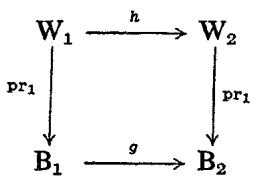
\includegraphics[keepaspectratio]{images/part001_9c3df15b.jpg}}

\(\mathbf{C}^{r}\) 类态射。设 \(\mathbf{W}_{1}\)（相应地，\(\mathbf{W}_{2}\)）是 \(\mathbf{B}_{1}\times\mathbf{F}_{1}\)（相应地，\(\mathbf{B}_{2}\times\mathbf{F}_{2}\)）的开子集，并设 \(h:\mathbf{W}_{1}\to\mathbf{W}_{2}\) 是一个映射。我们称 \(h\) 是一个 \(g\)-态射（\(\mathbf{C}^{r,s}\) 类的），如果 \(\mathrm{pr}_{1}\circ h=g\circ\mathrm{pr}_{1}\) 且 \(\mathrm{pr}_{2}\circ h\) 是 \(\mathbf{C}^{r,s}\) 类映射（15.1.6，从 \(\mathbf{W}_{1}\) 到 \(\mathbf{F}_{2}\)）。

类似地，设 \(B_{3}\) 是一个 \(C^{r}\) 类流形，\(W_{3}\) 是 \(B_{3} \times F_{3}\) 的开子集（其中 \(F_{3}\) 是一个 K-Banach 空间），并设 \(g'\) 是一个 \(C^{r}\) 类态射（从 \(B_{2}\) 到 \(B_{3}\)）。若 h（相应地，

\(h^{\prime})\)）是一个 \(g\)-态射（相应地，\(g^{\prime}\)-态射），是 \(\mathbf{C}^{r,s}\) 类的、从 \(\mathbf{W}_1\) 到 \(\mathbf{W}_2\)（相应地，从 \(\mathbf{W}_2\) 到 \(\mathbf{W}_3\)）的映射，则复合 \(h^{\prime} \circ h\) 是一个 \((g^{\prime} \circ g)\)-态射，是 \(\mathbf{C}^{r,s}\) 类的、从 \(\mathbf{W}_1\) 到 \(\mathbf{W}_3\) 的映射。

\subsection{\texorpdfstring{\(C^{r,s}\) 类流形（在 \(C^{r}\) 类流形之上）}{C\^{}\{r,s\} 类流形（在 C\^{}\{r\} 类流形之上）}}

在本节中，我们用 B 表示一个 \(C^{r}\) 类微分流形。

15.2.1. 设 X 是一个装备了映射 \(p: \mathbf{X} \to \mathbf{B}\) 的集合。我们称三元组 \(\theta = (\mathbf{V}, \psi, \mathbf{F})\) 为 X 在 B 上的卡，其中 V 是 X 的子集，F 是 K 上的 Banach 空间，\(\psi\) 是从 V 到 \(\mathbf{B} \times \mathbf{F}\) 的一个开子集上的双射，且满足 \(\mathrm{pr}_1 \circ \psi = p|\mathbf{V}\)。

设 \((\theta_{i})_{i\in I} = ((V_{i},\psi_{i},F_{i}))_{i\in I}\) 是 X 在 B 上的一个卡族。我们称诸 \(\theta_{i}\) 是 \(C^{r,s}\)-相容的，如果对 I 的每一对元素 \(i,j\)，下列两个条件都满足：

\begin{enumerate}
\def\labelenumi{\alph{enumi})}
\item
  \(\psi_i(V_i \cap V_j)\) 在 \(B \times F_i\) 中是开的，且 \(\psi_j(V_i \cap V_j)\) 在 \(B \times F_j\) 中是开的；
\item
  映射 \(\psi_i\circ\psi_j^{-1}\)（从 \(\psi_j(V_i\cap V_j)\) 到 \(\psi_i(V_i\cap V_j)\)）是一个 \(\mathrm{Id}_{\mathbf{B}}\)-态射，且是 \(\mathbf{C}^{r,s}\) 类的（15.1.7）。
\end{enumerate}

卡的一个族 \(((\mathrm{V}_i,\psi_i,\mathrm{F}_i))_{i\in I}\)（X 在 B 上的卡，它们 \(\mathbf{C}^{r,s}\)-相容且定义域 \(\mathrm{V}_i\) 覆盖 X）称为 X（在 B 上）的一个 \(\mathbf{C}^{r,s}\)-图册。两个 \(\mathbf{C}^{r,s}\)-图册称为等价的，如果它们的并仍是一个 \(\mathbf{C}^{r,s}\)-图册；\(\mathbf{C}^{r,s}\)-图册之间的等价关系是一个等价关系。\(\mathbf{C}^{r,s}\)-图册的一个等价类称为集合 X 上一个在 B 上的 \(\mathbf{C}^{r,s}\) 类流形结构；当希望指明 K 时，就写 \(\mathbf{C}_{\mathbb{K}}^{r,s}\) 以代替 \(\mathbf{C}^{r,s}\)。若 X 是 B 上的一个 \(\mathbf{C}^{r,s}\) 类流形，我们称 \(p\colon X\to B\) 为 X 的投影；若 \(\theta\) 是 X 在 B 上的一个卡，则我们称 \(\theta\) 是 \(\mathbf{C}^{r,s}\)-流形 X 的卡，如果 \(\theta\) 属于定义 X 结构的等价类中的某个图册。

设 X 是 B 上的一个 \(C^{r,s}\) 类流形，其投影为 p。则在 X 上存在

一个 \(\mathbf{C}^{r}\) 类微分流形结构，且是唯一的，使得对每个卡 \((V,\psi,F)\)（\(\mathbf{C}^{r,s}\)-流形 X 的卡），V 在 X 中是开的，且 \(\psi\) 是一个 \(\mathbf{C}^{r}\)-同构，它把 X 的开子流形 V 映到 \(\psi(V)\)（\(\mathbf{B}\times F\) 的开子流形）上。若给 X 装备这个结构，则映射 \(p:X\to B\) 是一个 \(\mathbf{C}^{r}\) 类的浸没。

设 \(b \in \mathbf{B}\)，并设 \(\mathbf{X}_b = p^{-1}(b)\)。存在一个 \(\mathbf{C}^s\) 类的 K-流形结构（\(\mathbf{X}_b\) 上的结构），且是唯一的，使得对每个卡 \(\theta = (\mathbf{V}, \psi, \mathbf{F})\)（\(\mathbf{C}^{r,s}\)-流形 \(\mathbf{X}\) 的卡），三元组 \(\theta_b = (\mathbf{V} \cap \mathbf{X}_b, \operatorname{pr}_2 \circ \psi | (\mathbf{V} \cap \mathbf{X}_b), \mathbf{F})\) 是流形 \(\mathbf{X}_b\) 的卡。这个结构之下的 \(\mathbf{C}^r\) 类微分流形结构是由上面定义的 \(\mathbf{C}^r\) 类微分流形结构（\(\mathbf{X}\) 上的结构）诱导的。
% semantic-fragments: legacy-input-seam
\relax{}
15.2.3. 例

\begin{enumerate}
\def\labelenumi{(\roman{enumi})}
\item
  当 B 退化为一点时，B 上的 \(C_{K}^{r,s}\) 类流形的概念等价于 \(C^{s}\) 类 K-流形的概念。
\item
  设 Z 是一个 \(C^{s}\) 类 K-流形；取 \(X = B \times Z\) 与 \(p = pr_{1}\)。在 X 上存在、且仅存在一个 B 上的 \(C^{r,s}\) 类流形结构，使得对 Z 的每个卡 \((U, \psi, L)\)，\((B \times U, Id_{B} \times \psi, L)\) 都是 \(C^{r,s}\) -流形 X 的一个卡。
\item
  设 X 是 B 上的一个 \(C^{r,s}\) 类流形，Y 是 X 的一个开子集。由 X 的结构诱导的 Y 的 \(C^{r,s}\) 类流形结构，其定义与流形情形中的做法相同（参见 5.2.3）。
\item
  设 M 是一个以 B 为底、\(C^{r}\) 类的 K 上的向量丛（7.3.4），\(\pi\) 是它到 B 上的投影。在 M 上存在、且仅存在一个 B 上的 \(C_{K}^{r,\omega}\) 类流形结构，使得若 \((\mathbf{U},\psi,\mathbf{F})\) 是 M 的一个 K-向量卡（8.8.1），则三元组 \((\pi^{-1}(\mathbf{U}),\psi,\mathbf{F})\) 是 \(C_{K}^{r,\omega}\) -流形 M 的一个卡。
\end{enumerate}

15.2.4. 设 X 是 B 上的一个 \(C^{r,s}\) 类流形，p 是其投影，L 是一个 K-Banach 空间，f 是 X 到 L 中的一个映射。我们说 f 是 \(C^{r,s}\) 类的，如果对流形 X 的每个卡 (V, \(\psi\) , F)（这里 X 视为 \(C^{r,s}\) -流形），映射 ( \(f|V) \circ \psi^{-1}\) （从 \(\psi(V)\) 到 L 中）是 \(C^{r,s}\) 类的（15.1.6）。这样的映射是 \(C^{r}\) 类的，并且它在 \(X_{b}\) （\(b \in B\)）上的限制是 \(C^{s}\) 类的。

15.2.5. 设 \(g: \mathbf{B} \to \mathbf{B}'\) 是 \(\mathbf{C}^{r}\) 类微分流形的一个态射，并设

\pandocbounded{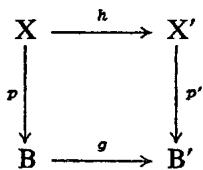
\includegraphics[keepaspectratio]{images/part001_9e08a31f.jpg}}

X（相应地，X'）是 B（相应地，B'）上的一个 \(C^{r,s}\) 类流形，h 是 X 到 X' 中的一个映射。我们说 h 是一个 \(C^{r,s}\) 类 g-态射，如果下列三个条件得到满足：

\begin{enumerate}
\def\labelenumi{\alph{enumi})}
\item
  \(p^{\prime}\circ h = g\circ p;\)
\item
  h 连续；
\item
  对每个卡 \((\mathrm{V}^{\prime},\psi^{\prime},\mathrm{F}^{\prime})\) （\(C^{r,s}\) -流形 \(X^{\prime}\) 的卡），映射 \(pr_{2}\circ\psi^{\prime}\circ h\) 从 \(V=h^{-1}(V^{\prime})\) 到 \(F^{\prime}\) 是
\end{enumerate}

\(\mathbf{C}^{r,s}\) 类的（按 15.2.4 的意义），这里开集 V 赋有由 X 诱导的结构（15.2.3, (iii)）。

当 \(\mathbf{B} = \mathbf{B}'\) 且 \(g = \mathrm{Id}_{\mathbf{B}}\) 时，我们也称 \(h\) 为一个 \(\mathbf{C}^{r,s}\) 类 B-态射。

为使一个 \(C^{r,s}\) 类 B-态射是一个 \(C^{r,s}\) 类 B-同构，只需它是一个 \(C^{1}\) 类同构。

设 \(g': B' \to B''\) 是 \(C^r\) 类流形的一个态射，并设 \(X''\) 是一个 \(C^{r,s}\) 类流形，其底为 \(B''\) 。若 \(h: X \to X'\) 是一个 \(g\) -态射且为 \(C^{r,s}\) 类，而 \(h': X' \to X''\) 是一个 \(g'\) -态射且为 \(C^{r,s}\) 类，则 \(h' \circ h\) 是一个 \((g' \circ g)\) -态射且为 \(C^{r,s}\) 类。

15.2.6. 设 X 是 B 上的一个 \(\mathbf{C}_{\mathbf{R}}^{r,s}\) 类流形，\(p\) 是其投影；我们假设 \(s \neq \omega\) ，X 是分离的，且 \(p\) 是逆紧的（TG, I, § 10, no. 1）。于是，对每个 \(b \in \mathbf{B}\) ，存在 \(b\) 的一个开邻域 U 以及一个 \(\mathbf{C}^{r,s}\) -同构（从 \(p^{-1}(\mathbf{U})\) 到 \(\mathbf{U} \times \mathbf{X}_b\) 上），其中 \(\mathbf{X}_b = p^{-1}(b)\) 。

15.2.7. 设 X 是 B 上的一个 \(C_{K}^{r,s}\) 类流形，p 是其投影，\(\sigma: B \to X\) 是一个 \(C^{r}\) 类截面。我们称一个 \(C_{K}^{r,s}\) 类管状邻域（\(\sigma\) 的）为如下的三元组 (M, N, \(\varphi\) )：其中 M 是一个以 B 为底、\(C^{r}\) 类的 K-向量丛，N 是 \(\sigma(\mathbf{B})\) 在 X 中的一个开邻域，而 \(\varphi\) 是一个 \(C_{K}^{r,s}\) 类 B-同构（从 N 到 M 的一个开子集上，参见 15.2.3 (iv)），它把截面 \(\sigma\) 映为 M 的零截面。

假设 \(s \geqslant r + 1\) ，并且流形 B 是仿紧的、具有 \(\mathbf{C}^{r}\) 类单位分解（5.3.6）；则存在 \(\mathbf{C}_{\mathbb{K}}^{r,s}\) 类管状邻域（\(\sigma\) 的）。

\subsection{截面簇与映射簇}

15.3.1（“截面空间上的 Banach 空间结构”）。设 B 是一个 \(C^{r}\) 类紧微分流形；设 M 是一个以 B 为底、\(C^{r}\) 类的 K 上的向量丛（7.3.4）；用 \(M_{r}\) 表示 M 的底层 \(C^{r}\) 类微分流形，并用 \(\mathcal{S}_{\mathrm{M}}^{\tau}(\mathrm{B})\) 表示 M 的 \(C^{r}\) 类截面所成的 K-向量空间（7.4.1）。在 \(\mathcal{S}_{\mathrm{M}}^{\tau}(\mathrm{B})\) 上，由 \(C^{r}\) -一致收敛拓扑（在 \(\mathcal{C}^{\tau}(\mathrm{B};\mathrm{M}_{r})\) 上，12.3.10）诱导的拓扑使 \(\mathcal{S}_{\mathrm{M}}^{\tau}(\mathrm{B})\) 成为一个 K-Banach 空间。

设 \((\mathrm{U}_{i})_{i\in\mathbb{I}}\) 是 B 的一个有限开覆盖，并且对每个 \(i\in I\) ，设 \(c_{i}=(\mathrm{U}_{i},\varphi_{i},\mathrm{E}_{i})\) 是 B 的一个卡，\(t_{i}=(\mathrm{U}_{i},\psi_{i},\mathrm{F}_{i})\) 是 M 的一个 K-向量卡（8.8.1）。设每个 \(E_{i}\) （相应地，\(F_{i}\) ）都赋有与它在 R（相应地，K）上的 Banach 空间结构相容的范数，并且 \((\mathrm{V}_{i})_{i\in\mathbb{I}}\) 是 B 的一个闭覆盖，使得 \(V_{i}\subset U_{i}\) 对所有 \(i\in I\) 成立。对 \(f\in\mathcal{S}_{\mathrm{M}}^{\tau}(\mathrm{B})\) 与 \(i\in I\) ，用 \(f_{i}\) 表示由 \(\varphi_{i}(\mathrm{U}_{i})\) 到 \(F_{i}\) 的映射，它由下述复合得到：

\[
\varphi_ {i} \left(\mathrm{U} _ {i}\right) \xrightarrow {\varphi_ {i} ^ {- 1}} \mathrm{U} _ {i} \xrightarrow {f} \mathrm{M} \left| \mathrm{U} _ {i} \xrightarrow {\psi_ {i}} \mathrm{U} _ {i} \times \mathrm{F} _ {i} \xrightarrow {\operatorname{pr} _ {2}} \mathrm{F} _ {i}. \right.
\]

规定

\[
\| f \| = \operatorname{Sup} _ {i \in I, p \leqslant r, x \in V _ {i}} \| D ^ {p} f _ {i} (\varphi_ {i} (x)) \|.
\]

映射 \(f\mapsto\|f\|\) 是 \(\mathcal{S}_{\mathrm{M}}^{\tau}(\mathrm{B})\) 上的一个范数，它给 \(\mathcal{S}_{\mathrm{M}}^{\tau}(\mathrm{B})\) 一个 K 上的 Banach 空间结构。

若 N 是空间 M 的一个开子集，则集合 \(\mathcal{S}^{\tau}(\mathbf{B};\mathbf{N})\) （由截面 \(f\in\mathcal{S}_{\mathbf{M}}^{\tau}(\mathbf{B})\) 中满足 \(f(\mathbf{B})\subset\mathbf{N}\) 者组成）在 \(\mathcal{S}_{\mathbf{M}}^{\tau}(\mathbf{B})\) 中是开的。

15.3.2. 设 B 是一个 \(C^{r}\) 类紧微分流形，X 是 B 上的一个 \(C_{K}^{r,s}\) 类（ \(s \geqslant r + 1\) ）流形。若 N 是 X 的一个开子集，则用 \(\mathcal{S}^{r}(B; N)\) 表示 B 上的像含于 N 的 \(C^{r}\) 类截面所成的集合。在 \(\mathcal{S}^{r}(B; X)\) 上存在、且仅存在一个 \(C^{s-r}\) 类 K-流形结构，使得对每个截面 \(\sigma \in \mathcal{S}^{r}(B; X)\) 以及每个管状邻域 (M, N, \(\varphi\) )（\(C_{K}^{r,s}\) 类，\(\sigma\) 的，15.2.7），三元组 ( \(\mathcal{S}^{r}(B; N)\) , \(\varphi^{*}\) , \(\mathcal{S}_{M}^{r}(B)\) )——其中 \(\varphi^{*}\) 是映射 \(f \mapsto \varphi \circ f\) ——是 K-流形 \(\mathcal{S}^{r}(B; X)\) 的一个卡。

在下文中，我们给 \(\mathcal{S}^{r}(\mathbf{B};\mathbf{X})\) 赋以这一结构。

15.3.3. 设 X 是一个 \(C^{r}\) 类紧微分流形，Y 是一个 \(C^{s}(s \geqslant r + 1)\) 类 K-流形。设 \(\mathcal{C}^{r}(X; Y)\) 是从 X 到 Y 中的 \(C^{r}\) 类映射所成的集合（换句话说，取值于 Y 的底层 \(C^{r}\) 类流形中，参见 5.13.1 与 5.14.2）。我们给 \(\mathcal{C}^{r}(X; Y)\) 赋以一个 \(C^{s-r}\) 类 K-簇结构，它由与 \(\mathcal{S}^{r}(X; X \times Y)\) 的等同得到（参见 15.2.3, (ii) 与 15.3.2）。称它为从 X 到 Y 中的 \(C^{r}\) 类映射簇。它的拓扑是 \(C^{r}\) -一致收敛拓扑（12.3.10）。

假设 Y 是分离的；则 \(\mathcal{C}^{r}(X;Y)\) 也是分离的。此外，从 X 到 Y 中的 \(C^{r}\) 类浸入（相应地，嵌入、浸没、满射浸没、平展态射、同构）所成的集合是 \(\mathcal{C}^{r}(X;Y)\) 的一个开子集。

设 \(X'\) 是一个 \(C^r\) 类紧微分流形，\(\varphi: X' \to X\) 是 \(C^r\) 类微分流形的一个态射，而 \(\psi: Y \to Y'\) 是 \(C^s\) 类 K-簇的一个态射。映射 \(f \mapsto \psi \circ f \circ \varphi\) 是一个 \(C^{s-r}\) 类态射（从 \(\mathscr{C}^r(X; Y)\) 到 \(\mathscr{C}^r(X'; Y')\) 中）。

15.3.4（“结构弱化”）。保留 15.3.3 的假设与记号。此外，设 \(s' \in \mathbf{N}_{\mathbf{R}}\) 满足 \(r < s' \leqslant s\) ，并设 \(\mathbf{Y}_{s'}\) 是一个 \(\mathbf{C}^{s'}\) 类实流形，它以 \(\mathbf{Y}\) 为底层（5.13 与 5.14.2）。\(\mathbf{C}^{s'-r}\) 类实流形结构（在 \(\mathcal{C}^r(\mathbf{X}; \mathbf{Y}_{s'})\) 上）是 \(\mathbf{C}^{s-r}\) 类 K-流形结构（在 \(\mathcal{C}^r(\mathbf{X}; \mathbf{Y})\) 上）的底层。

15.3.5. 设 X 与 X' 分别是 \(C^{r}\) 类与 \(C^{r'}\) 类的紧微分流形，且 \(r' < r\) ；设 Y 是一个 \(C^{s}\) 类 K-簇，\(s \geqslant r + 1\) 。令 \(t = \operatorname{Inf}(r - r', s - r)\) 。映射 \((f, g) \mapsto g \circ f\) 是一个 \(C^{t}\) 类态射（从 \(\mathcal{C}^{r}(X'; X) \times \mathcal{C}^{r}(X; Y)\) 到 \(\mathcal{C}^{r'}(X'; Y)\) 中）。

15.3.6（“\(\mathcal{C}^r (\mathrm{X};\mathrm{Y})\) 的切空间”）。在 15.3.3 的假设之下，设 \(f\in \mathcal{C}^r (\mathrm{X};\mathrm{Y})\) ，并设 \(\xi\) 是 \(f\) 处切于流形 \(\mathcal{C}^r (\mathrm{X};\mathrm{Y})\) 的一个切向量。若 \(x\in \mathrm{X}\) ，则用 \(\varepsilon_{x}\) 表示映射 \(g\mapsto g(x)\) （从 \(\mathcal{C}^r (\mathrm{X};\mathrm{Y})\) 到 Y 中）；它是一个 \(\mathbf{C}^{s - r}\) 类态射。\(\xi\) 在 \(\mathrm{T}_f(\varepsilon_x)\) 下的像是一个元素 \(\xi_{x}\) ，它属于 \(\mathrm{T}_{f(x)}(\mathrm{Y})\) ；映射 \(x\mapsto \xi_{x}\) 是一个 \(\mathbf{C}^r\) 类提升，即 \(f\) 在 T(Y) 中的提升（参见 8.6.1），并且可以把它与一个 \(\mathbf{C}^r\) 类截面（属于以 X 为底的向量丛 \(f^{*}\mathrm{T}(\mathrm{Y})\)）等同起来。这样，就得到了切空间 \(\mathrm{T}_f(\mathcal{C}^r (\mathrm{X};\mathrm{Y}))\) 到 Banach 空间 \(\mathcal{S}_{f^{*}\mathrm{T}(\mathrm{Y})}^r (\mathrm{X})\) 上的一个同构。

15.3.7（“\(\mathcal{C}^{p}(\mathrm{X};\mathcal{C}^{q}(\mathrm{Y};\mathrm{Z}))\) 的解释”）。设 X 与 Y 分别是 \(\mathbf{C}^{p}\) 类与 \(\mathbf{C}^{q}\) 类的紧微分流形（ \(1\leqslant p\leqslant+\infty,1\leqslant q<+\infty\) ），并设 Z 是一个 \(\mathbf{C}^{s}\) 类 K-簇，\(s\geqslant p+q\) 。设 \(f\colon\mathrm{X}\times\mathrm{Y}\to\mathrm{Z}\) 是一个连续映射；

对每个 \(x \in X\) ，用 \(f_x\) 表示从 Y 到 Z 的映射 \(y \mapsto f(x, y)\) 。下列两个性质等价：

\begin{enumerate}
\def\labelenumi{\alph{enumi})}
\item
  对任意卡 \(c = (\mathrm{U}, \varphi, \mathrm{E})\) （\(\mathbf{X}\) 的）、任意卡 \(d = (\mathrm{V}, \psi, \mathrm{F})\) （\(\mathbf{Y}\) 的）与任意卡 \(e = (\mathrm{W}, \theta, \mathrm{G})\) （\(\mathbf{Z}\) 的），只要 \(f(\mathrm{U} \times \mathrm{V}) \subset \mathrm{W}\) ，偏导数 \(\mathrm{D}_{\mathbb{E}}^{p'} \mathrm{D}_{\mathbb{F}}^{q'} f'\) （其中 \(f'\) 是 \(f\) 在卡 \(c \times d\) 与 \(e\) 中的表达式，5.3.2）对 \(p' \leqslant p\) 与 \(q' \leqslant q\) 都存在且连续。
\item
  对每个 \(x \in X\) ，映射 \(f_{x}\) 是 \(C^{q}\) 类的，且映射 \(x \mapsto f_{x}\) 是一个 \(C^{p}\) 类态射（从 X 到簇 \(\mathcal{C}^{q}(Y; Z)\) 中）。
\end{enumerate}

\pandocbounded{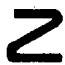
\includegraphics[keepaspectratio]{images/part001_50717dae.jpg}}

15.3.8. 设 Y 是一个 \(C^{s}\) 类紧 K-簇，\(s \geqslant r + 1\) ，并设 \(\text{Diff}^{r}(Y)\) 是 Y 的底层 \(C^{r}\) 类实流形 \(Y_{r}\) 的 \(C^{r}\) 类自同构所成的群。集合 \(\text{Diff}^{r}(Y)\) 在 \(\mathcal{C}^{r}(Y; Y) = \mathcal{C}^{r}(Y_{r}; Y)\) 中是开的；我们给它赋以一个 \(C^{s-r}\) 类 K-簇结构（由 \(\mathcal{C}^{r}(Y; Y)\) 诱导）。复合律 \((f, g) \mapsto g \circ f\) 使 \(\text{Diff}^{r}(Y)\) 成为一个拓扑群。另一方面，\(C^{s-r}\) 类流形结构一般说来与 \(\text{Diff}^{r}(Y)\) 的群结构不相容。对 \(f \in \text{Diff}^{r}(Y)\) ，映射 \(g \mapsto g \circ f\) （从 \(\text{Diff}^{r}(Y)\) 到其自身）是 \(C^{s-r}\) 类的，但映射 \(g \mapsto f \circ g\) 一般说来不是 \(C^{1}\) 类的。特别地，\(\text{Diff}^{r}(Y)\) 一般说来不是一个李群。\footnote{假设 \(s = \infty\)。设 \(\text{Diff}^{\infty}(Y)\) 是 Y 的 \(C^{\infty}\) 类自同构所成的群；给它赋以使诸典范单射 \(\text{Diff}^{\infty}(Y) \to \text{Diff}^{r}(Y)\)（对每个整数 \(r \geqslant 1\)）都连续的最粗拓扑。另一方面，设 \(\text{Diff}^{0}(Y)\) 是 Y 的同胚所成的群，赋以一致收敛拓扑（TG, X, § 3, no. 5, 命题 11）。若 \(\dim Y \geqslant 1\)，则不可能找到一个李群 G 以及从 \(\text{Diff}^{\infty}(Y)\) 到 G 和从 G 到 \(\text{Diff}^{0}(Y)\) 的连续同态，使其复合恰为典范单射（参见 LIE, III, § 4, 习题 7）。}

\specialchapter{记号索引}

\(N_{K}\) : 记号与约定 T(X): 8.1.1 \(\zeta_{c}\) : 8.1.1 T(f): 8.1.2 T(X/Y): 8.1.3 \((\partial/\partial u^{i})\) : 8.1.5 T'(X): 8.2.2 df: 8.2.2 \(\langle\xi, df\rangle\) , D \(_{\xi}(f)\) , \(\xi(f)\) : 8.2.3 \(\varphi^{*}\eta\) : 8.2.6 \(\varphi^{*}\omega\) : 8.2.7 与 8.3.1 \(^{k}\Omega^{p}(U; E)\) : 8.3.1 \(\omega|Y\) : 8.3.1 \(\omega\wedge\omega'\) : 8.3.2 \(i(\xi,\omega)\) , \(i(\xi)\omega\) , \(i(\xi).\omega\) : 8.3.2 \(d\omega\) : 8.3.5 GL(E): 8.4.1 \(\theta_{\xi}.f\) : 8.4.2 \([\xi,\eta]\) : 8.5.1 \(i(\psi,\omega)\) , \(i(\psi)\omega\) , \(i(\psi).\omega\) : 8.6.2 F ⊗ C: 8.8.2 T'(X), T''(X): 8.8.3 Alt \(^{p,q}\) (T(X); F): 8.8.4 \(\omega_{p,q}\) : 8.8.4 \(d'\omega\) , \(d''\omega\) : 8.8.5 \(\partial/\partial z^{k}\) , \(\partial/\partial\bar{z}^{k}\) : 8.8.10 \(dz^{\Delta}\) , \(d\bar{z}^{\Delta}\) : 8.8.10 \(\alpha_{+}\) , \(\alpha_{-}\) , \(\Omega\) : 9.1.4 \(\rho\) , \(\Delta\) : 9.1.5 \(X_{p}\) : 9.2.1 T(X,Y): 9.2.8 F': 9.3.7 \(\xi^{p}\) : 9.4.1 \(\Lambda_{p}(x,y)\) : 9.4.2

\(\mu^{\otimes n}, \mu_{\mathrm{U}}^{\otimes n}: 10.1\)

mod(a): 10.1

Jac(f): 10.1.1

mod(\(\omega\))\(_{\mu}\), \(|\omega|\): 10.1.6

\(\xi'\xi''\), \(\xi''\xi': 10.2.1\)

Or(E): 10.2.1

\(\mathrm{Or}_{\mathrm{M}}\): 10.2.2

\(\lambda_{\mathrm{M}} = (\mathrm{Or}_{\mathrm{M}}, \{\pm 1\}, \mathrm{X}, \pi)\): 10.2.2

\(\tilde{\mathbf{X}}\): 10.2.4

\(\xi_1 \otimes \xi_2: 10.2.6\) \(\tilde{\mathbf{R}}_{\mathrm{M}}\): 10.3.1

\(\tilde{\mathbf{R}}_{\mathbf{X}}\): 10.4.1

\(\alpha(\omega), \int_{\mathbf{X}} g \cdot \omega, \int_{\mathbf{A}} \omega: 10.4.3\) \(\omega|_{\mathrm{Y}}: 10.4.3\) \(\partial A: 11.1.2\) 与 11.3.2

\(\mathrm{T}_a^+(\mathrm{A}), \mathrm{T}_a^-(\mathrm{A}): 11.1.4\) \(\omega|_{\partial A}: 11.2.2\) \(u \perp (t_1, \ldots, t_p): 11.4.1\) \(\tilde{\mathbf{R}}_n: 11.4.2\) \(\omega \perp (t_1, \ldots, t_p): 11.4.5\) \(\int_{\pi|_{\mathrm{A}}} \omega, \int_{\pi} \omega: 11.4.6\) \(j_x^k(f): 12.1.2\) \(s(j), b(j): 12.1.2\) \(\mathrm{J}^k(\mathrm{X}, \mathrm{Y}), \mathrm{J}_x^k(\mathrm{X}, \mathrm{Y}), \mathrm{J}^k(\mathrm{X}, \mathrm{Y})_y, \mathrm{J}_x^k(\mathrm{X}, \mathrm{Y})_y: 12.1.2\) \(j' \circ j: 12.1.4\) \(r^{k, k'}(j): 12.1.5\) \(j_x^\infty(f), j_x^\omega(f): 12.1.6\) \(\mathrm{P}_m(\mathrm{E}; \mathrm{F}): 12.2\) \(\Delta^m f(a), \Delta_a^m(f), \Delta_a^m(j): 12.2.1\) \(\mathrm{Q}^k(\mathrm{E}, \mathrm{F}): 12.2.2\) \(\mathrm{T}(j): 12.3.4\) \(j^k(f): 12.3.7\) \(\mathrm{J}^k(f, g): 12.3.9\) \(\mathrm{GL}^k(\mathrm{E}): 12.4.2\) \(\mathrm{R}^k(\mathrm{E}, \mathrm{X}): 12.4.3\) \(\mathrm{P}_x^k(\pi), \mathrm{P}^k(\pi): 12.5.1\) \(\mathrm{P}^k(g): 12.5.3\) \(\mathrm{P}^k(\mathrm{E}): 12.6.1\) \(\mathrm{P}^k(\mathrm{X}): 12.6.2\) \(\mathrm{P}^k(u): 12.6.3\) \(\tau_m(\mathcal{V}), \tau_m(f), \mathrm{P}_m(\mathrm{E}; \mathrm{F}): 12.6.7\) \(\mathrm{TS}^n(\mathrm{E}), \mathrm{TS}(\mathrm{E}), \mathrm{TS}^{(r)}(\mathrm{E}), \mathrm{TS}^{(r)+}(\mathrm{E}): 13.1.1\) \(\gamma_n(x): 13.1.1\) \(\langle f, t\rangle\): 13.1.2, 13.1.3, 13.2.2, 13.6.1

\(\varphi_{*}(t)\) : 13.1.4 \(\mathrm{T}_x^{(r)}(\mathrm{X}), \mathrm{T}_x^{(k)}(\mathrm{X}), \mathrm{T}_x^{(k)+}(\mathrm{X})\) : 13.2.1 \(\varepsilon_x\) : 13.2.1 \(\langle j, t \rangle\) : 13.2.2 \(\mathrm{T}_x^{(r)}(\varphi), \varphi_*\) : 13.2.3, 13.6.1 \(\mathrm{T}^{(k)}(\mathrm{X}), \mathrm{T}^{(k)+}(\mathrm{X})\) : 13.2.5 \((\Delta_{\xi}^{\alpha})_a\) : 13.2.6 \(\mathrm{gr}_k \mathrm{T}_x^{(r)}(\mathrm{X}), \mathrm{gr} \mathrm{T}_x^{(r)}(\mathrm{X})\) : 13.3.1 \(i, i_x, i_X, i_{X,x}\) : 13.3.1 \(i_k\) : 13.3.1 \(\mathrm{gr}(\varphi_x)\) : 13.3.5 \(t_1 \times t_2, t_1 \otimes t_2\) : 13.4.1 \(\mathrm{T}_x^{(n)}(\mathrm{X}_1, \mathrm{X}_2)\) : 13.4.5 \(\Delta_*\) , \(c\) : 13.5.1 \(\mathcal{T}^{(k)}(\mathrm{X})\) : 13.6.1 \(\mathrm{D}^k (\mathrm{E}, \mathrm{F})\) : 14.1.1 \(\mathcal{D}_{\mathrm{U}}^{k,h}(\mathrm{E}, \mathrm{F})\) : 14.1.1 \(\operatorname{ad}(f)\theta\) : 14.1.4 \(\Delta^\alpha\) : 14.1.6 \(\mathrm{D}_{\mathbf{C}}^{k}(\mathrm{E}, \mathrm{F})\) : 14.1.7 \(\mathrm{D}'' \circ \mathrm{D}'\) : 14.1.8 \([\mathrm{D}' , \mathrm{D}'']\) : 14.1.8 \(\mathrm{S}^k (\mathrm{E}, \mathrm{F})\) : 14.2.1 \(\sigma_k (\mathrm{D})\) : 14.2.1 \(\mathrm{Sym}^k (\mathrm{M}; \mathrm{N})\) : 14.2.2 \(\Omega, \tilde{\mathbf{M}}\) : 14.3.1 \(^t\mathbf{D}\) : 14.3.2 \(\Omega_1, \mathbf{G}\) : 14.3.4 \(\Omega^p\) : 14.4.2 \(\operatorname{grad}(f)\) : 14.4.3 \(\mathbf{C}_{\mathbf{R}}^{r,s}\) : 15.1.1 \(\mathbf{C}_{\mathbf{K}}^{r,\omega}\) : 15.1.2 \(\mathbf{C}^{r,s}\) : 15.1.1, 15.1.2, 15.1.6, 15.2.1 \(\mathcal{S}_{\mathbf{M}}^r (\mathbf{B})\) : 15.3.1 \(\mathcal{S}^r (\mathbf{B}; \mathbf{N})\) : 15.3.1 与 15.3.2 \(\mathcal{C}^r (\mathbf{X}; \mathbf{Y})\) : 15.3.3\\
Diff'(Y): 15.3.8

\specialchapter{术语索引}

适配于块的（卡）：11.1.2 向量丛结构的弱化：8.7.1 积分弧、最大积分弧：9.1.3 C-向量图册、复向量图册：8.8.1 闭半空间的边界：11.1.1 块的边界：11.1.2 边界（带边界的流形）：11.1. 注（1） \(\mathbf{C}^{r,s}\) 类 B-态射：15.2.5 射流的靶：12.1.2 B 上 \(\mathbf{C}^{r,s}\) 类流形的卡：15.2.1 C-向量卡、复向量卡：8.8.1 B 上的卡：15.2.1 Cauchy（公式）：11.2.5 点分布场：13.2.5 \(\mathbf{C}^s\) 类点分布场：13.2.5 向量场：8.2.1 复向量场：8.8.2 余向量场：8.2.2 初始场：8.4.5 \(\mathbf{C}^0\) 类（流形、态射）：记号与约定 \(\mathbf{C}^{r,s}\) 类（函数）：15.1.1 与 15.1.2 \(\mathbf{C}^{r,s}\) 类（映射）：15.1.6 与 15.2.4. \(\mathbf{C}^{r,s}\) 类（g-态射）：15.1.6 与 15.2.5 B 上 \(\mathbf{C}^{r,s}\) 类（流形）：15.2.1 测度的典范类：10.1.4 微分算子的类：14.1.1 向量丛的复化：8.8.2 \((p,q)\) 型分量：8.8.4 两个射流的复合：12.1.4 两个微分算子的复合：14.1.8 共轭（截面）：8.8.2 ≥k 阶接触：12.1.1 无限阶接触：12.1.6 反变（函子）：8.2.7

点分布的余积：13.5.1 积分曲线：9.1.1 与 9.1.7 括号：8.5.1 \(\mathbf{C}^{r,s}\) -相容的（B 上的卡）：15.2.1 \(\mathbf{C}^{r,s}\) -图册：15.2.1 C-向量（丛、卡、图册）：8.8.1 闭半空间：11.1.1 函数的微分：8.2.2 外微分：8.3.5 与 10.3.4 有限支撑集的分布：13.6.1, 13.6.2 有限支撑集的复分布：13.6.2 点分布：13.2.1 阶 ≤k 的点分布：13.2.1 无常数项的分布：13.2.1 叶：9.2.2 连通叶：9.2.2 叶状结构：9.2.2 离散叶状结构、粗叶状结构：9.2.4 诱导叶状结构、逆像：9.2.5 叶化的（卡）：9.2.7 叶状的（流形）：9.2.2 余切丛：8.2.2 C-向量丛：8.8.1 法丛：8.1.3 切丛：8.1.1 纤维的切丛：8.1.3 相对切丛：8.1.3 横截丛：8.1.3 复向量丛：8.8.1 实向量丛：8.8.1 积分流：9.1.2 微分形式：8.3.1 交错微分形式：8.3.1 最大次数的微分形式：10.1.5 全纯（微分形式、向量场）：8.8.9 水平（截面）：9.2.10 奇（微分形式）：10.4.1 诱导（微分形式）：8.3.1 与 11.2.2 可积（向量子丛）：9.3.2 与 9.4.4 可积（微分形式）：10.4.3 局部可积（微分形式）：10.4.3 积分（叶状结构）：9.3.2 积分（子流形）：9.3.1 积分（全微分方程的）：9.3.7 向量子丛的积分：9.3.1

沿纤维的积分：11.4.6 寿命区间：9.1.3 雅可比：10.1.1 射流：12.1.2 无限阶射流：12.1.6 截面的射流：12.5.1 微分形式的模：10.1.6 局部可积模：10.1.5 M-扭曲（微分形式）：10.3.3 M-扭曲（标量丛）：10.3.1 可忽略（局部可忽略集）：10.1.3 Green 算子：14.3.4 复微分算子：14.1.7 有界阶的微分算子：14.1.1 E → F 型、阶 ≤k 的微分算子：14.1.1 多重微分算子：14.1.11 微分算子的阶：14.1.1 可定向（向量丛）：10.2.3 可定向（流形）：10.2.4 由复结构确定的定向：10.2.7 流形的定向：10.2.4 向量丛的定向：10.2.3 态射的定向：10.2.5 定向（定向空间）：10.2.2 偶（微分形式）：10.4.1 块：11.1.2 多面体（部分）：11.3.1 局部多面体（部分）：11.3.1 齐次多项式（映射）：13.1.2 殆复（结构）：8.8.3 定向的乘积：10.2.6 外积：8.3.2 内积：8.3.2 与 8.6.2 B 上 \(\mathbf{C}^{r,s}\) 类流形的投影：15.2.1 正则（点、边界）：11.3.2 提升：8.6.1 内向（向量、严格内向向量）：11.1.4 k 阶标架：12.4.3 切标架：8.1.5 Sard（定理）：10.1.3 标量（微分算子）：14.1.6 标量（多重微分算子）：14.1.11 纤维化的截面：记号与约定 S-态射的 S-定向：11.4.3 外向（向量、严格外向向量）：11.1.4

射流的源：12.1.2

Stokes（公式）：11.2.3 与 11.3.4

微分形式的支撑集：10.4.3

微分算子的符号：14.2.1

切（丛）：8.1.1

与叶状结构相切的（子丛）：9.2.8

点分布的常数项：13.2.1

扭曲（微分形式）：10.4.1

一致 \(C^{k}\) 收敛拓扑：12.3.10

扭曲（标量丛）：10.4.1

微分算子的转置：14.3.2

\((p,q)\) 型（微分形式）：8.8.4

\(\mathbf{C}^r\) 类映射流形：15.3.3

速度：9.1.1

管状邻域：15.2.7

π-扭曲（微分形式）：11.4.2

\(\varphi\)-相关：8.2.6



\end{document}
